 \documentclass[12pt]{article}
\renewcommand{\baselinestretch}{1.1}

%%% Add packages here
\usepackage{graphicx} 
%\usepackage{parskip}
\usepackage[table]{xcolor}
\usepackage{amsmath}
%\usepackage{float}
\usepackage{placeins} % prevent float
\usepackage{geometry}
\geometry{legalpaper, portrait, margin=3cm}
\usepackage{makecell}
\usepackage{multirow}
\usepackage{array}
\usepackage{amsfonts}
\usepackage{amsthm}
\usepackage{amssymb}
\usepackage{latexsym}
\usepackage{color}
\usepackage{verbatim}
\usepackage{fancyhdr}
\usepackage{fancybox}
\usepackage{listings}
\usepackage{threeparttable} % for table notes
\usepackage{hologo} % for TeX engine logos
\usepackage{booktabs} % for nice tables
\usepackage{longtable} % for longer tables
\usepackage[table,xcdraw]{xcolor}  % for color in tables
\usepackage{appendix} % for appendix
\usepackage{biblatex}
\addbibresource{references.bib}

\usepackage{amsmath} % for pseudo code
\usepackage{algorithm}
\usepackage{algpseudocode}
\usepackage{subcaption} % For subfigures
\usepackage{threeparttable} % for table notes

%%% Margins
\addtolength{\oddsidemargin}{-.50in}
\addtolength{\evensidemargin}{-.50in}
\addtolength{\textwidth}{1.0in}
\addtolength{\topmargin}{-.40in}
\addtolength{\textheight}{0.80in}

%%% Header
\pagestyle{fancy}
\chead{} % Clear undefined \groupname
\rhead{}
\lhead{}
\cfoot{\thepage}
\renewcommand{\headrulewidth}{0.4pt}

%%%%%%%%%%%%%%%%%%%%%%%%%%%%%%%%%%%%%

\begin{document}
\clearpage\thispagestyle{empty}

\begin{titlepage}

\begin{center}
\vspace*{1in}
	% title
	\centering\textbf{\huge{Bayesian data analysis project\\[1cm]
 }} \\[2cm]
	% details
	\Large{
	Master of Statistics and Data Science \\
	Hasselt University\\	
        2024-2025 \\
	}


\vspace*{3cm}
\textbf{\large{Group :}}\\
Luong Vuong (2365900) \\
Edward Owinoh (2365191) \\
Joseph Kaunda (2364031) \\



\vspace*{2cm}


\vspace*{1.5cm}
\textbf{\large{Lecturers:}}\\
Prof. Dr. Christel Faes \\
Dr. Oswaldo Gressani \\


\vspace*{2\baselineskip}
\today

\begin{figure}[b]
   \centering
   
\includegraphics[width=8cm]{pictures/UHasselt_logog.png}
   \label{fig:Uhasselt}
\end{figure}

\end{center}

\end{titlepage}

\section{Part 1}

\subsection{Model 1}

\subsubsection{Assumed model}
The number of participants in the screening program are modelled without covariates following the model formulation:

\[
    Y_{iag} \sim Binom(\pi_{i}, N_{iag})
\]

where $Y_{iag}$ is the number of participants amongst the $N_{iag}$ number of invited individuals, in municipality $i$ of age $a$ and gender $g$. $\pi_{i}$ is the participation rate per municipality. This means that the number of participants $Y_{iag}$ follows a Binomial distribution dependent on:

\begin{itemize}
    \item the number of invited individuals for each municipality-age-gender combination
    \item the participation rate per municipality. This participation rate is assumed to be averaged over the municipality regardless of the age or gender. 
\end{itemize}

\subsubsection{Model specification}

% The model assumes a conjugate non-informative Jeffreys prior (essentially a beta distribution with $\alpha$ = $\beta$ = $\frac{1}{2}$) for the participation rate $\pi_i$:

% \[
%     \pi_{i} \sim Beta(\alpha=\frac{1}{2}, \beta=\frac{1}{2})
% \]

The model assumes a conjugate beta prior for the participation rate $\pi_i$:

\[
    \pi_{i} \sim Beta(\alpha=1.0, \beta=1.0)
\]

\noindent implying no strong prior beliefs about the participation rate for the $i$th municipality. Three chains with a size of 10,000 iterations and a burn-in of 5,000 iterations were used. The thinning rate was left to the default value of 5. The starting values for the $\pi$ parameter in the first, second and third chains were set at 0.1, 0.5 and 0.9 respectively repeated over the 300 municipalities. The parameter to be monitored was $\pi_i$ and deviance (automatically provided). 

\subsubsection{Assessing convergence}

Various graphical and formal diagnostic checks were used to check for convergence of the Markov chains. These diagnostics and the findings are as follows:

\textbf{Trace plot}: The posterior distribution is rapidly explored by all chains for deviance and all $\pi_i$ in all chains. There are no gross deviations from stationarity. The sample traceplots are shown in figure \ref{fig:traceplotsm1}.

\begin{figure}[h!]
    \centering
    % First row
    \begin{subfigure}{0.45\textwidth}
        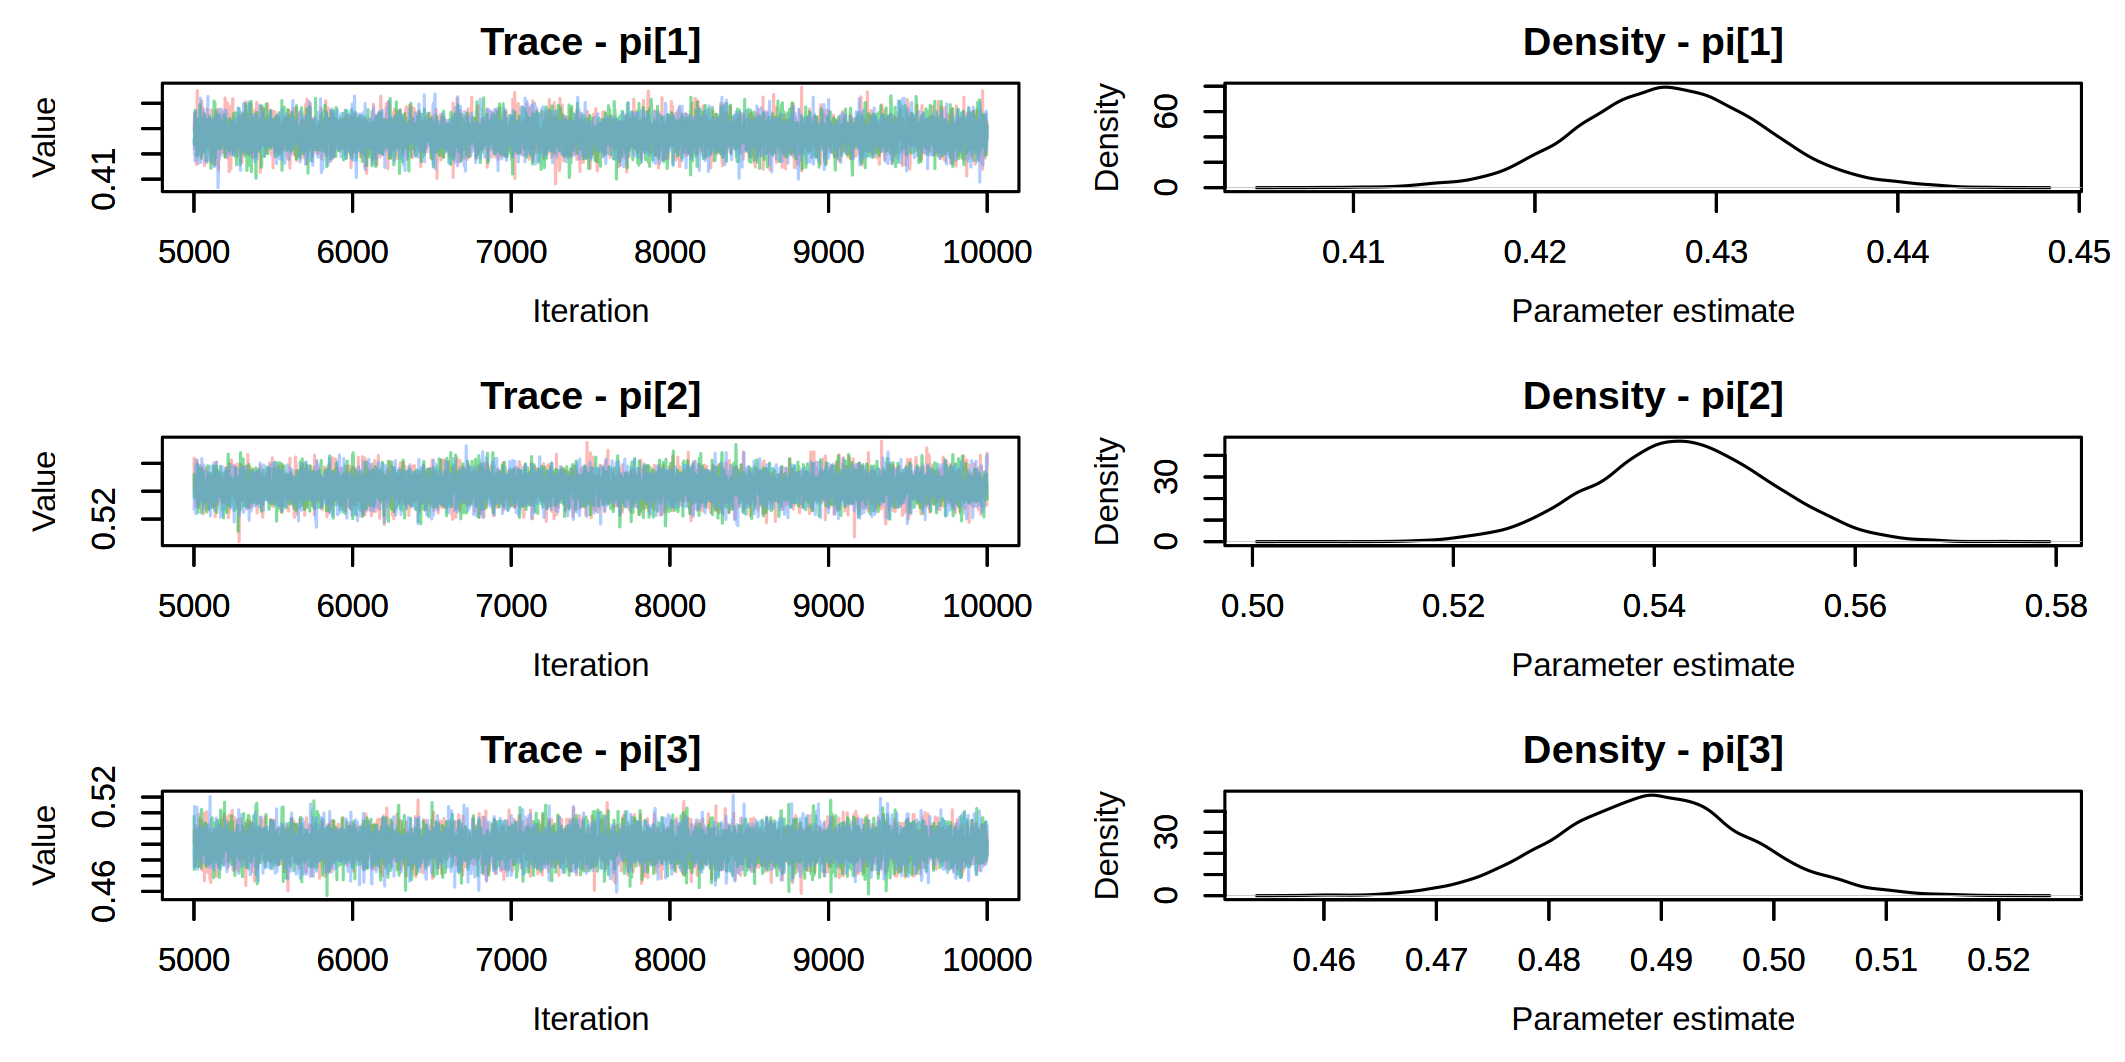
\includegraphics[width=\linewidth]{pictures/traceplot1-3.png}
        %\caption{pi[1:20]}
        %\label{fig:sub1_1}
    \end{subfigure}
    %\hfill
    \begin{subfigure}{0.45\textwidth}
        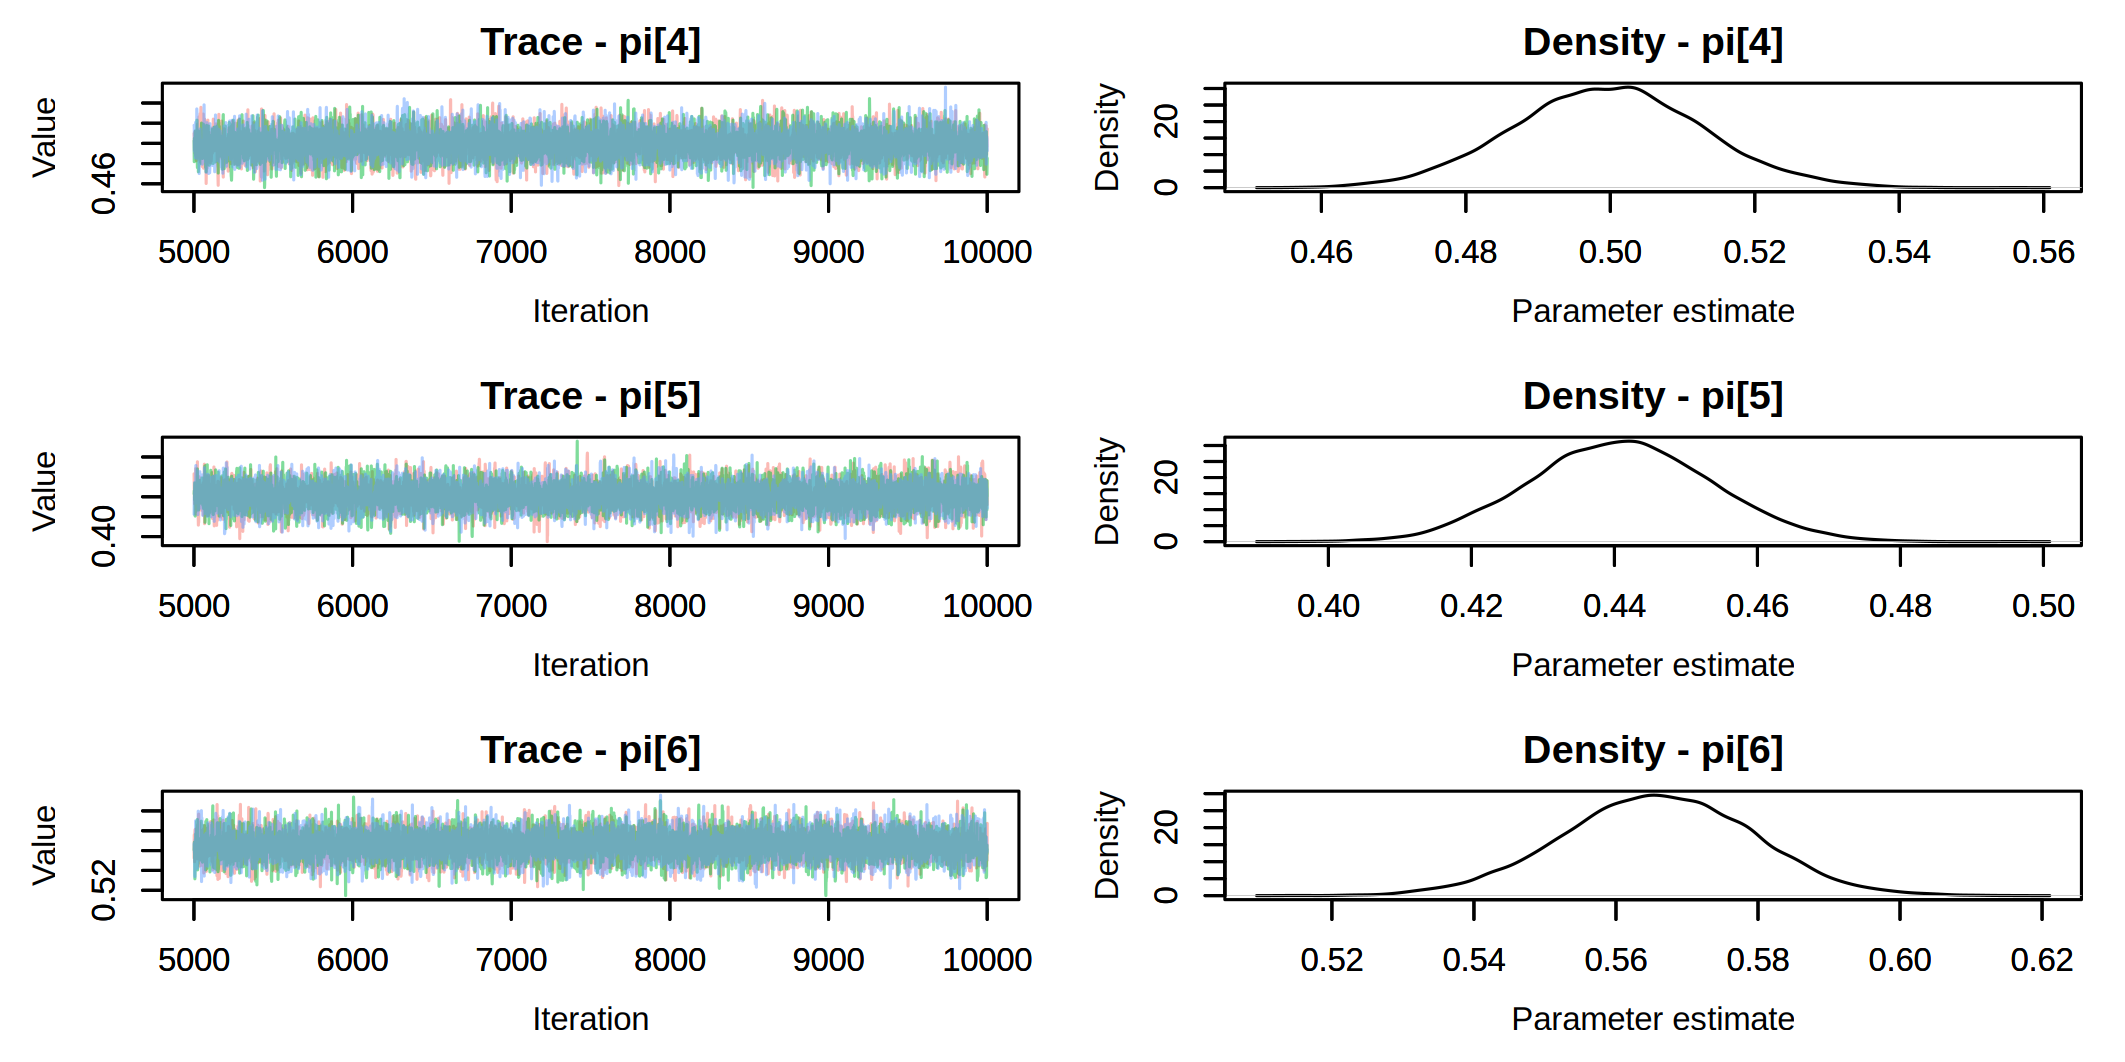
\includegraphics[width=\linewidth]{pictures/traceplot4-6.png}
        %\caption{pi[21:40]}
        %\label{fig:sub1_2}
    \end{subfigure}
    
    \caption{Sample traceplots for $\pi_i$}
    \label{fig:traceplotsm1}
\end{figure}

\textbf{Autocorrelation plot}: The autocorrelation plots (sample in figure \ref{fig:autocorrM1}) show good mixing rates for all $\pi_i$ and deviance.

\begin{figure}[h!]
    \centering
    % First row
    \begin{subfigure}{0.45\textwidth}
        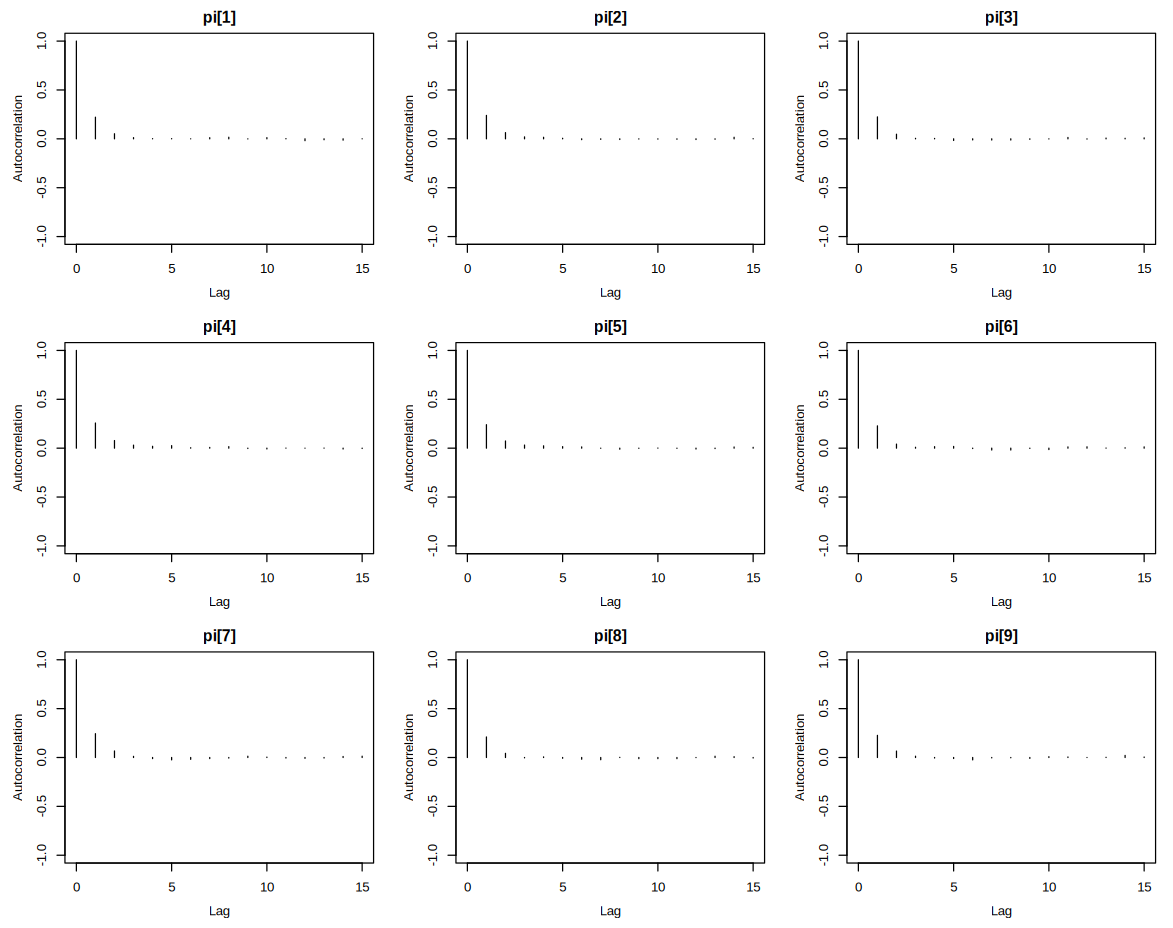
\includegraphics[width=\linewidth, height=8cm]{pictures/autocorr1.png}
        %\caption{pi[1:20]}
        %\label{fig:sub1_1}
    \end{subfigure}
    %\hfill
    \begin{subfigure}{0.45\textwidth}
        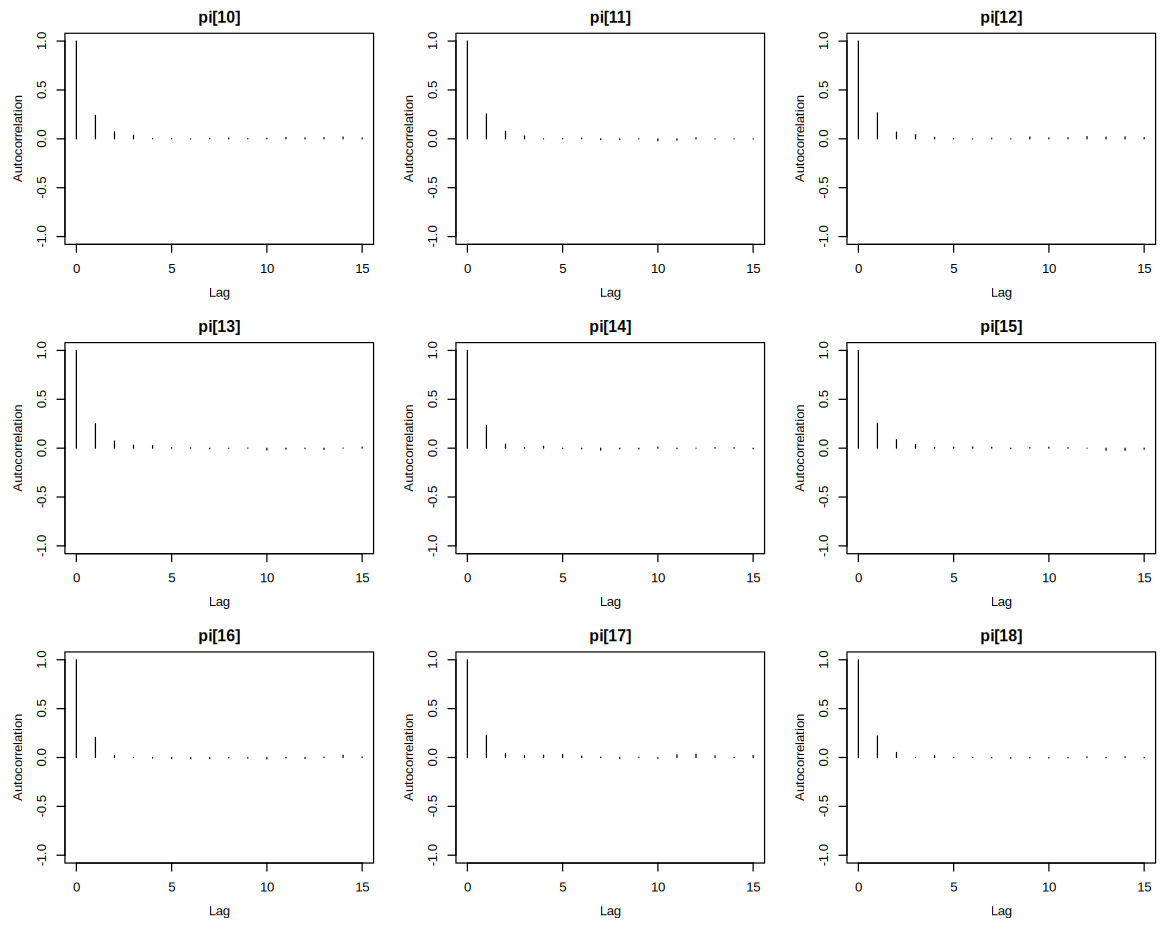
\includegraphics[width=\linewidth, height=8cm]{pictures/autocorr2.png}
        %\caption{pi[21:40]}
        %\label{fig:sub1_2}
    \end{subfigure}
    \caption{Sample autocorrelation plots for $\pi_i$}
    \label{fig:autocorrM1}
\end{figure}
\FloatBarrier % Ensures the figure doesn't float past this point

\textbf{Running-mean plots}: The running-mean plots (sample in figure \ref{fig:runningmeanM1}) show a stable behaviour for deviance all $\pi_i$ indicating stationarity.

\begin{figure}[h!]
    \centering
    % First row
    \begin{subfigure}{0.45\textwidth}
        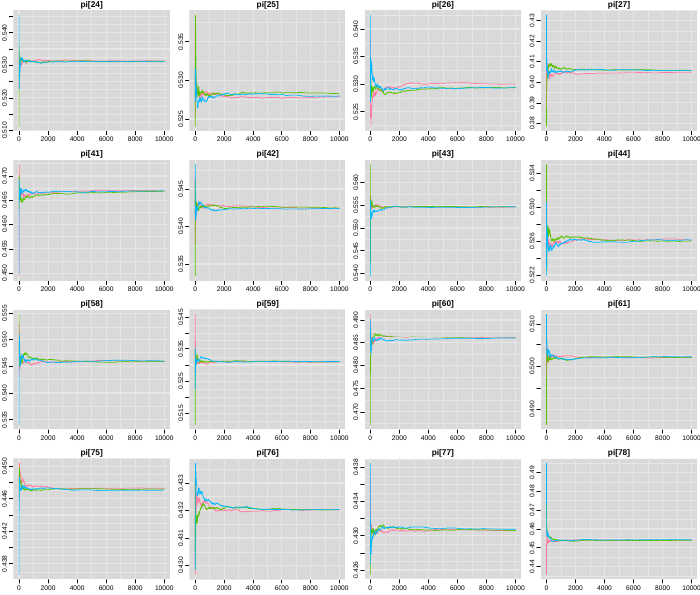
\includegraphics[width=\linewidth, height=8cm]{pictures/rmean2.png}
        %\caption{pi[1:20]}
        %\label{fig:sub1_1}
    \end{subfigure}
    %\hfill
    \begin{subfigure}{0.45\textwidth}
        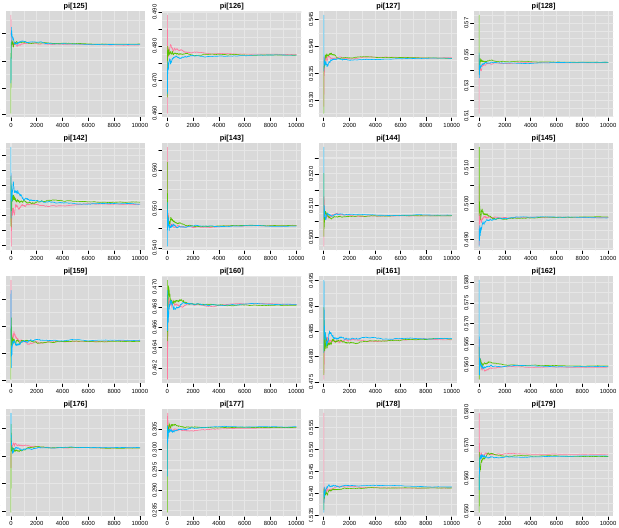
\includegraphics[width=\linewidth, height=8cm]{pictures/rmean3.png}
        %\caption{pi[21:40]}
        %\label{fig:sub1_2}
    \end{subfigure}
    
    \caption{Sample running-mean plots for $\pi_i$}
    \label{fig:runningmeanM1}
\end{figure}
\FloatBarrier % Ensures the figure doesn't float past this point

\textbf{Geweke diagnostic}: With the dynamic version of the Geweke diagnostic, most of the Z-values for $\pi_i$ and all Z-values for deviance in all chains fell inside the [-1.96, 1.96] interval indicating stationarity. A sample of the Geweke diagnostic plots are shown in figure \ref{fig:gewekem1}. 

\begin{figure}[h!]
    \centering
    % First row
    \begin{subfigure}{0.45\textwidth}
        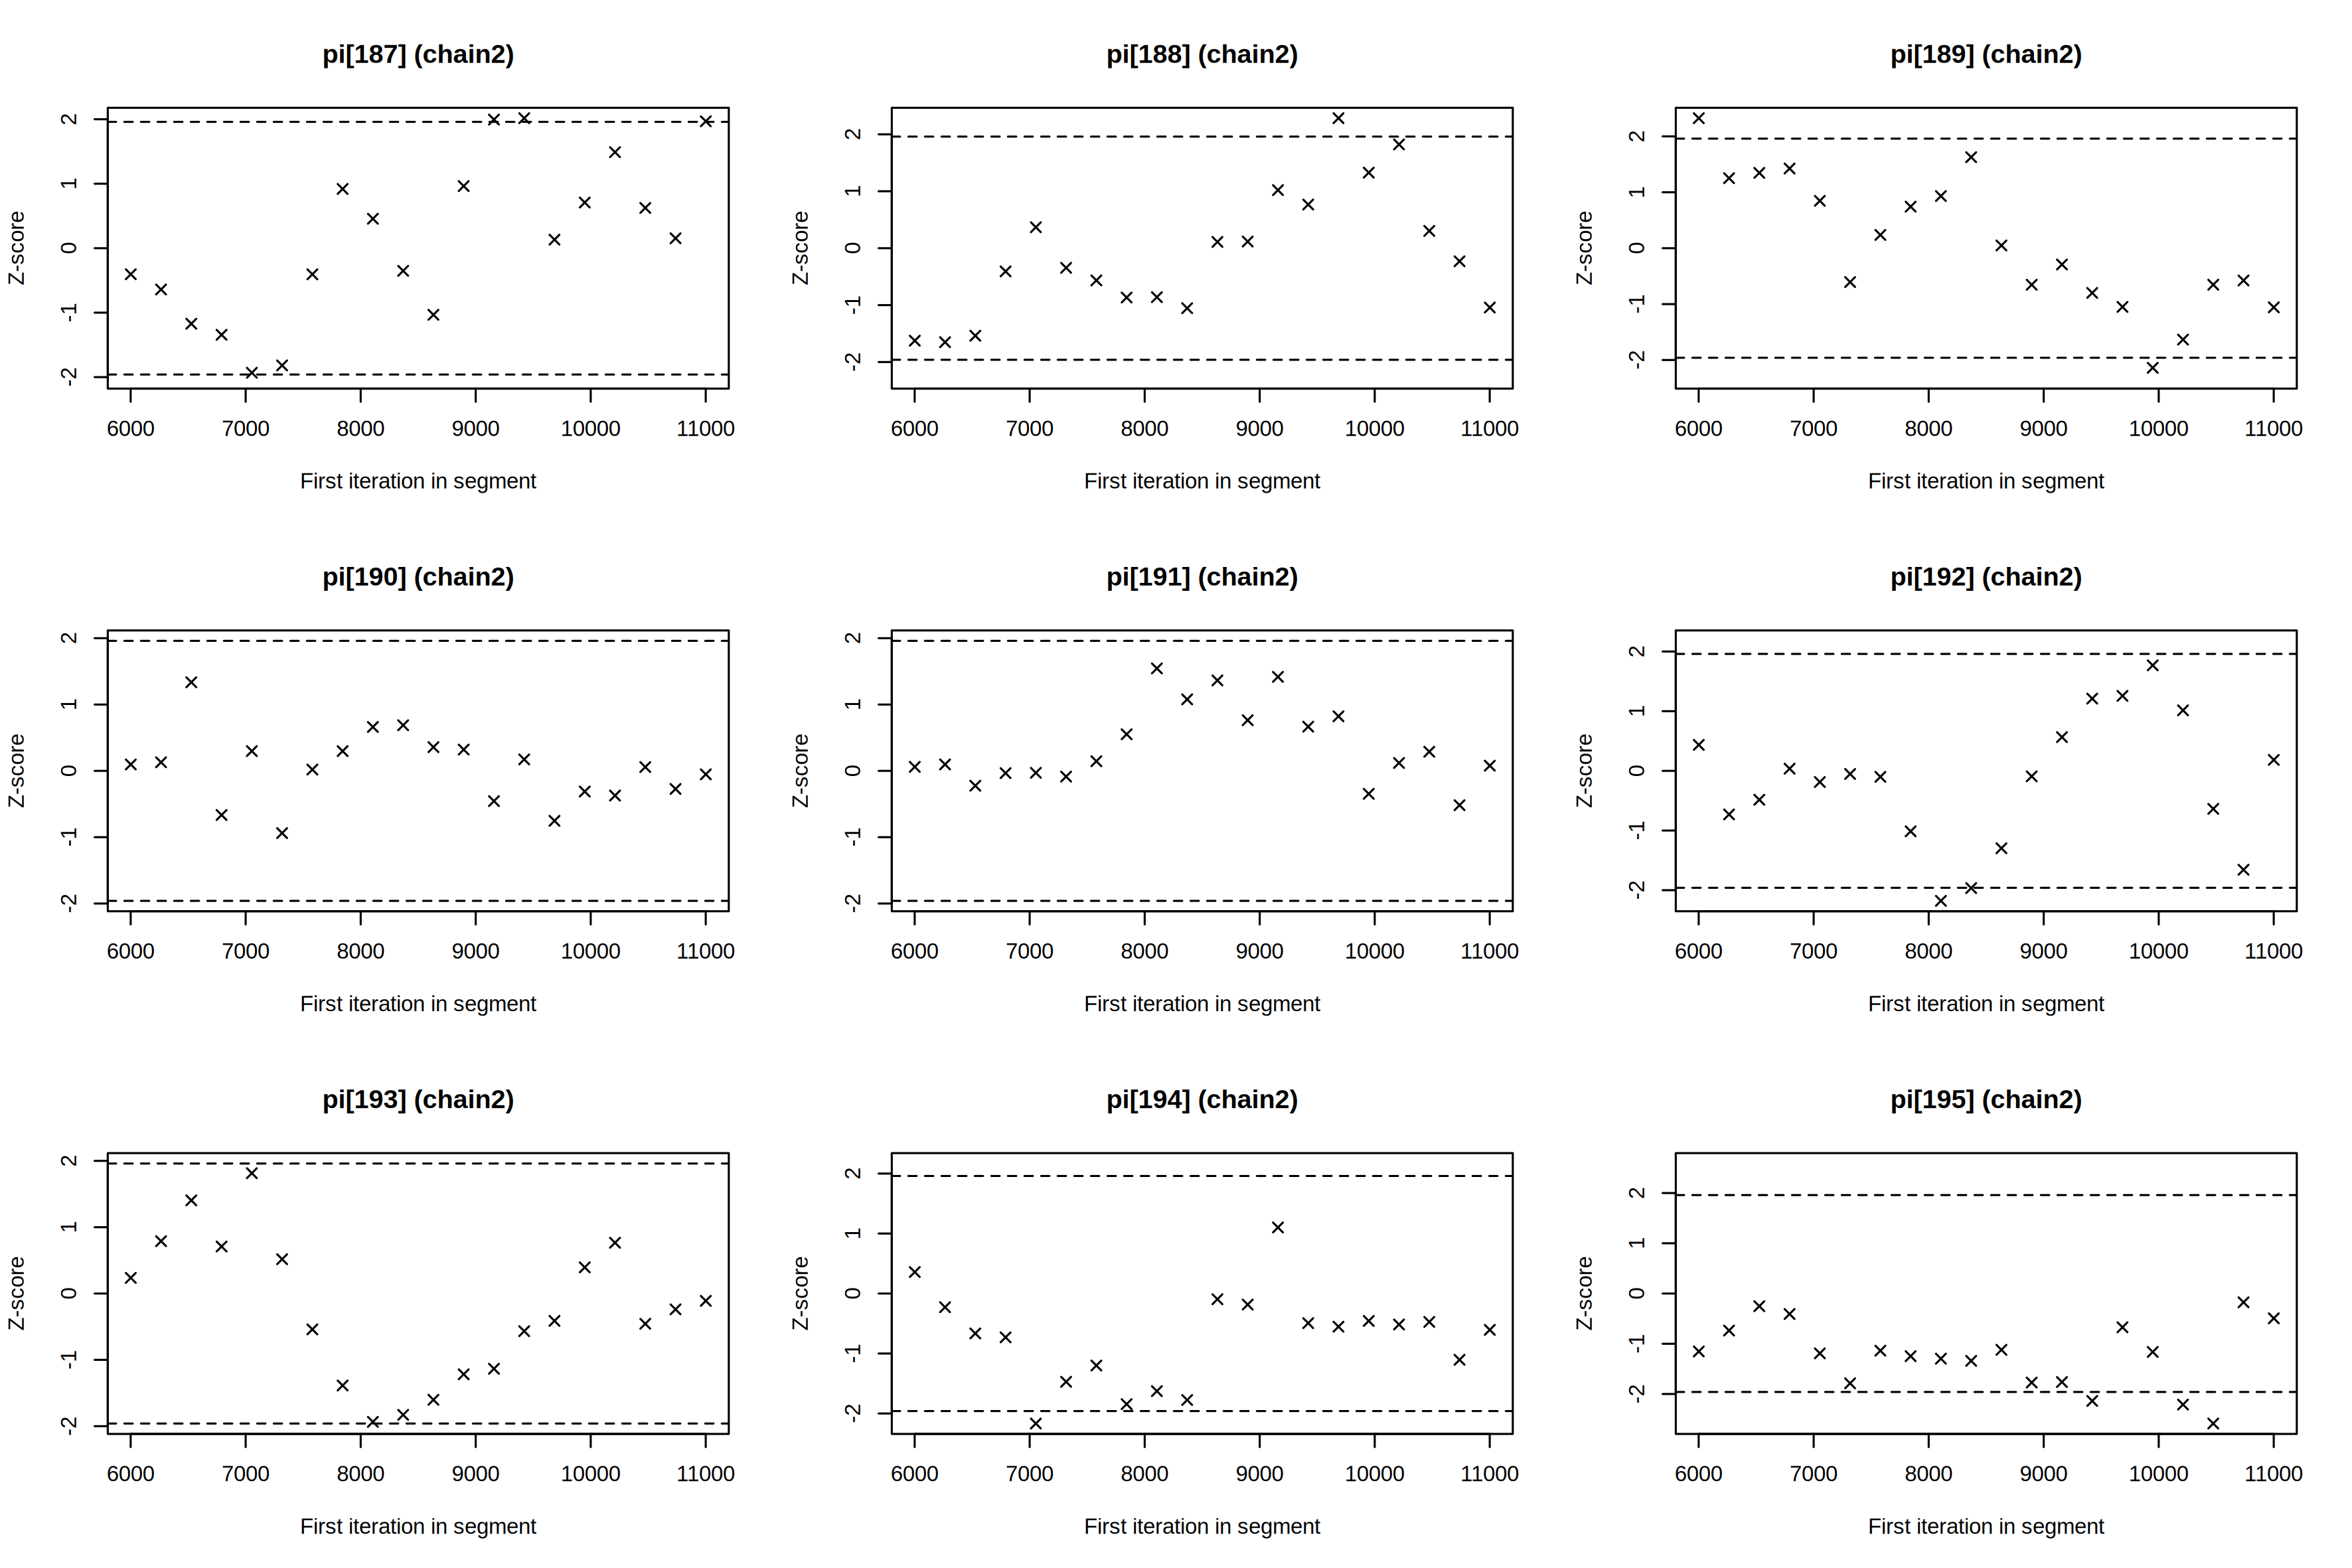
\includegraphics[width=\linewidth]{pictures/geweke187-195.png}
        %\caption{pi[1:20]}
        %\label{fig:sub1_1}
    \end{subfigure}
    %\hfill
    \begin{subfigure}{0.45\textwidth}
        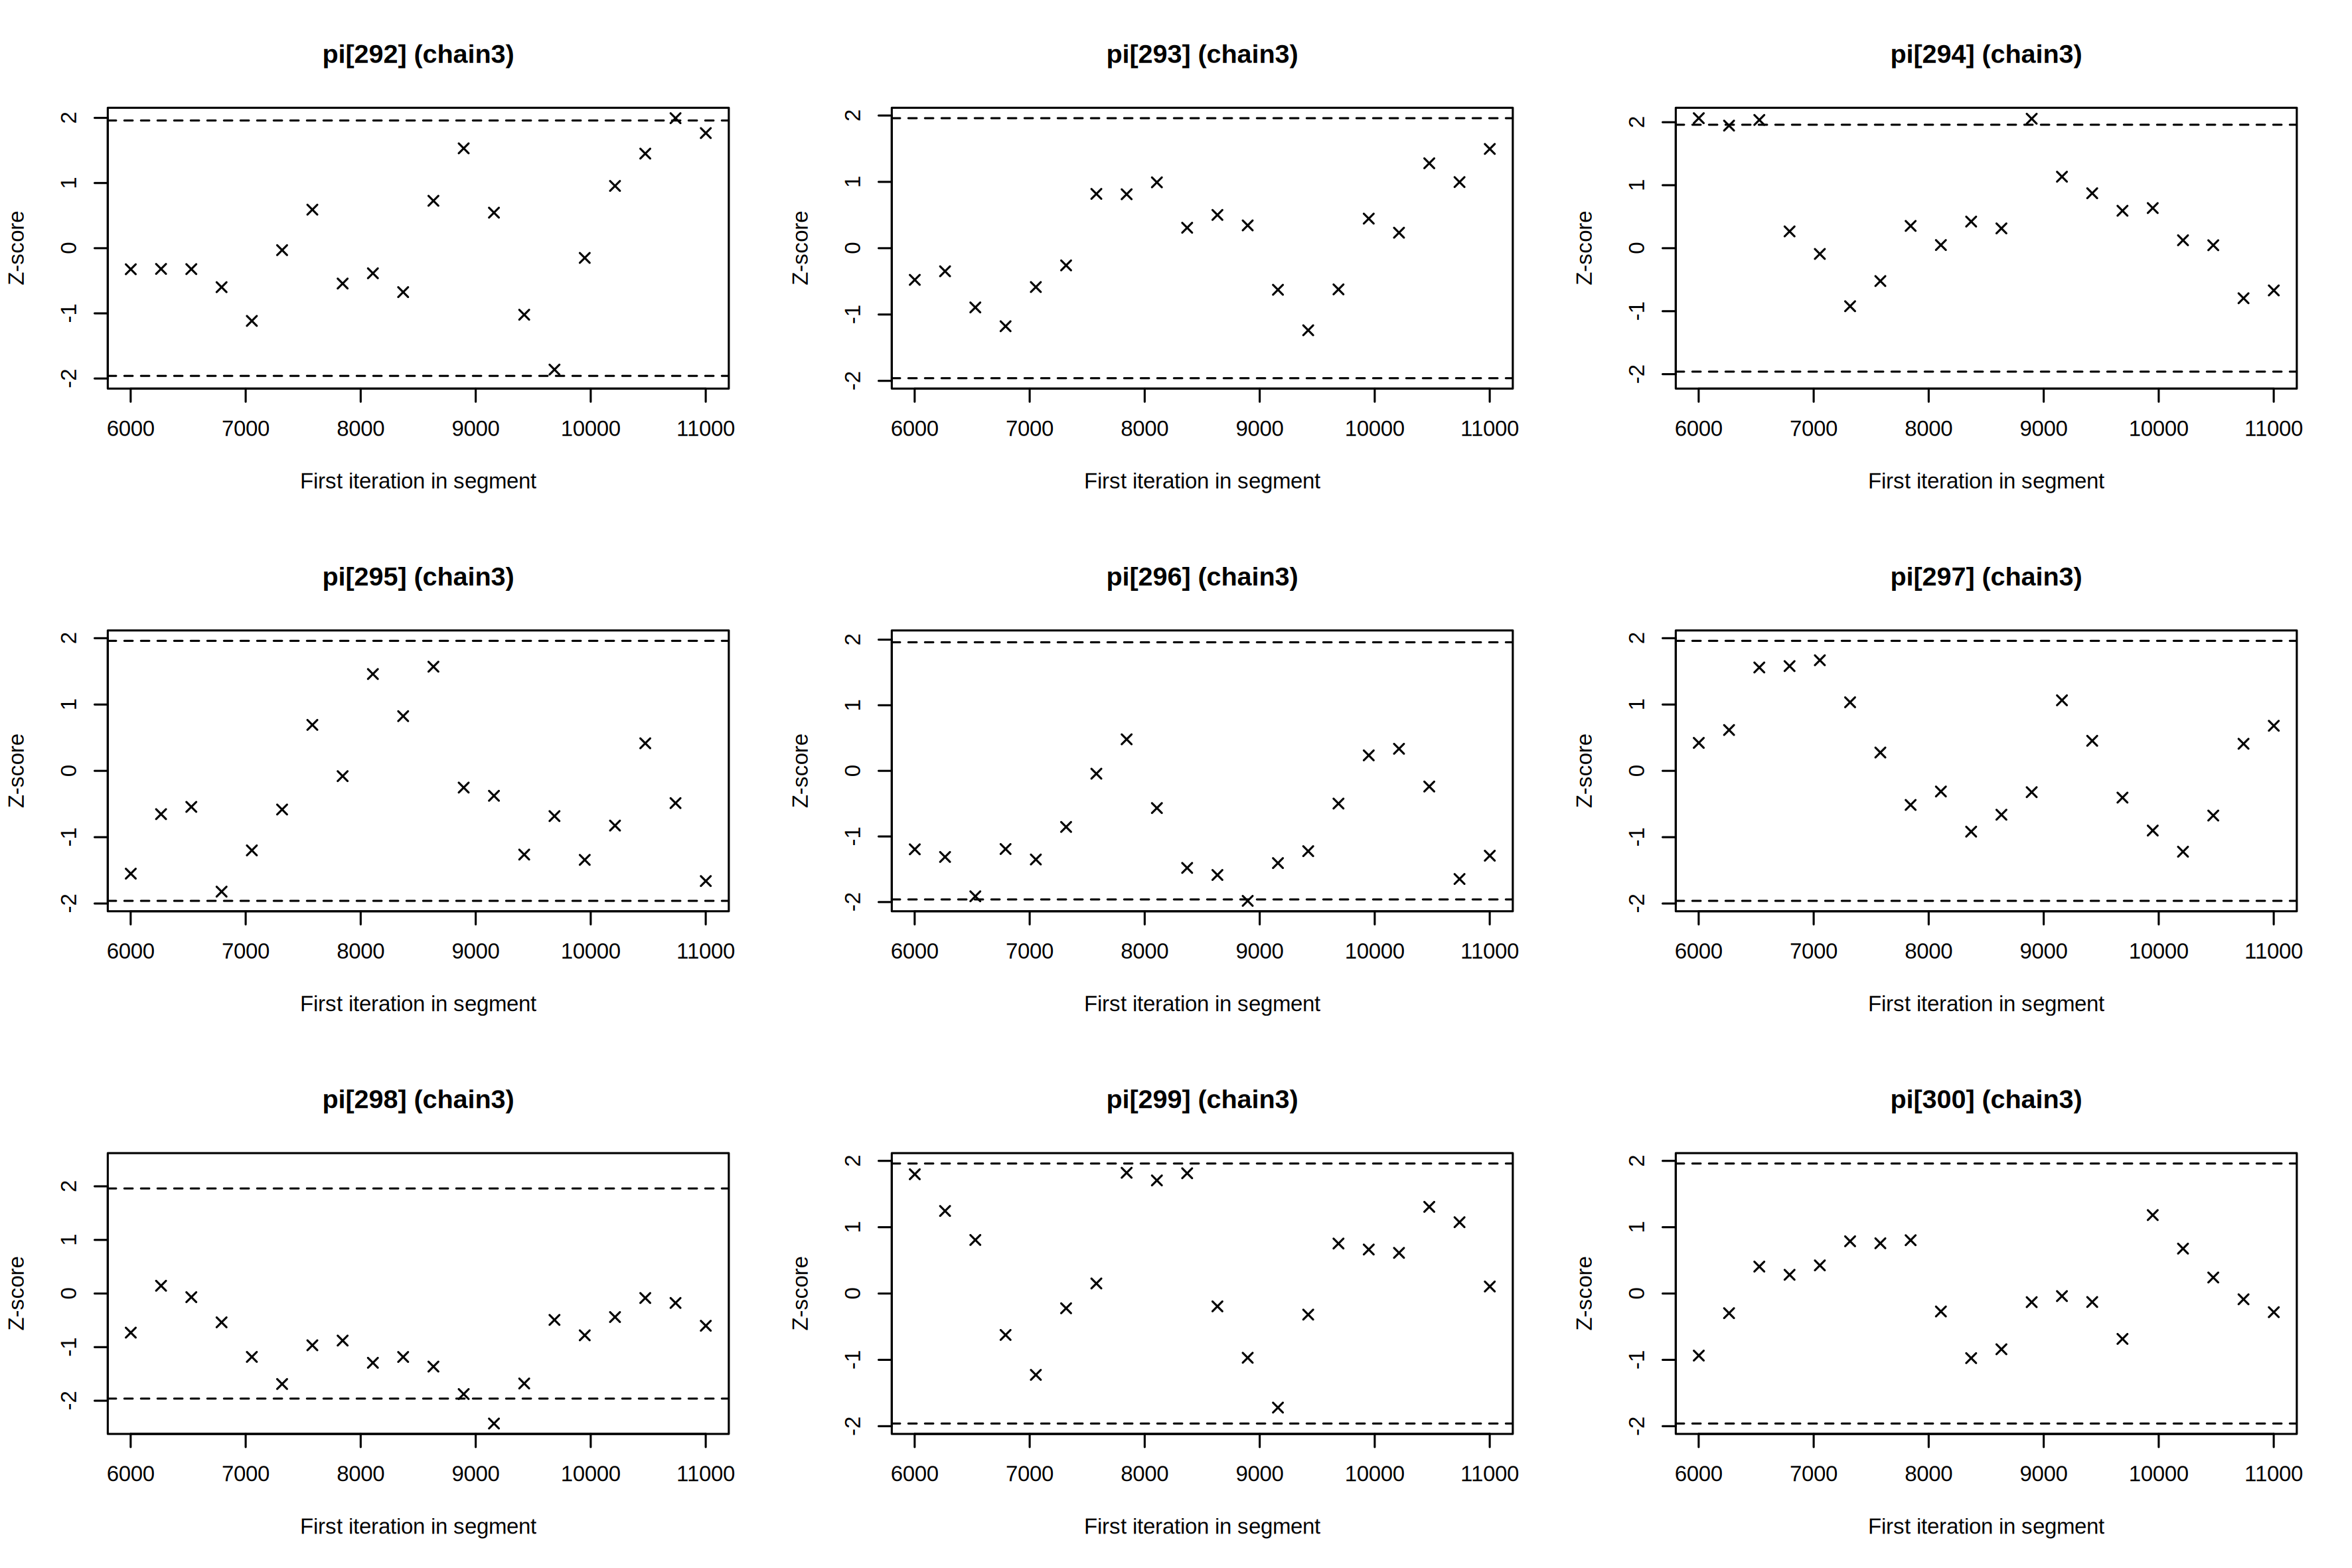
\includegraphics[width=\linewidth]{pictures/geweke292-300.png}
        %\caption{pi[21:40]}
        %\label{fig:sub1_2}
    \end{subfigure}
    
    \caption{Sample Geweke diagnostic for $\pi_i$}
    \label{fig:gewekem1}
\end{figure}

\textbf{Brooks–Gelman–Rubin (BGR) diagnostic}: With the dynamic version of the GR interval diagnostics, the curves stabilized almost immediately and no further iterations appeared necessary. For deviance and all $\pi_i$, the estimate of the potential scale reduction factor (psrf), $\hat{R_c}$ = 1 (with 97.5\% upper bound equal to 1). The multivariate psrf is 1.01.

\begin{figure}[h!]
    \centering
    % First row
    \begin{subfigure}{0.45\textwidth}
        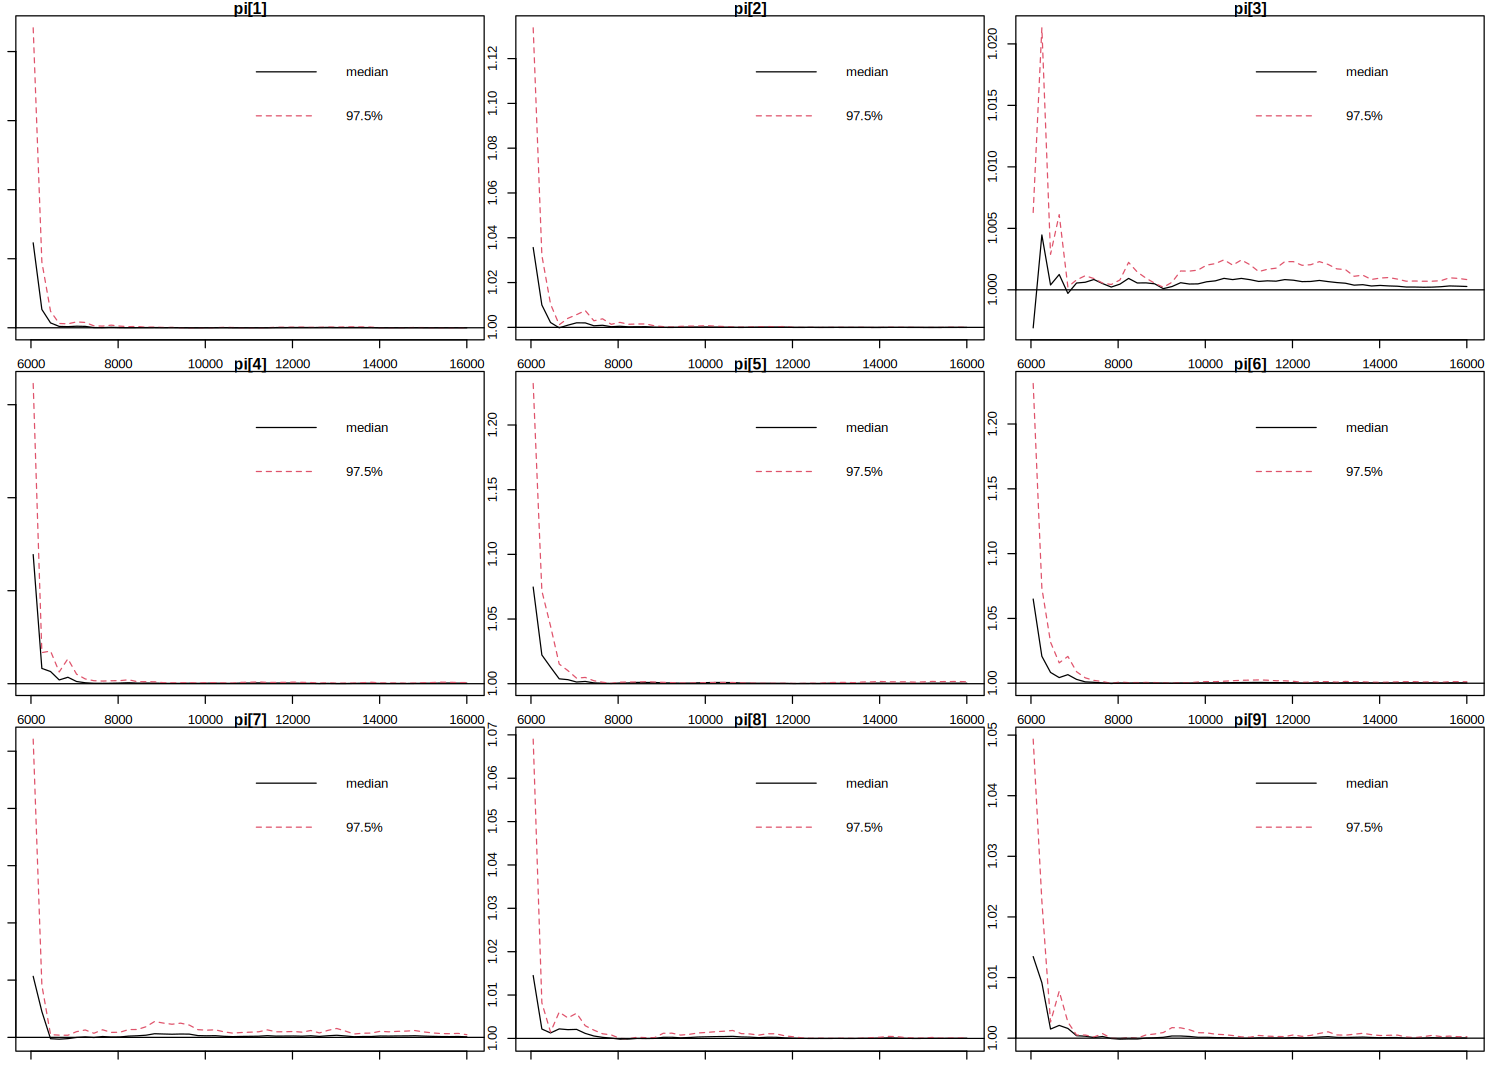
\includegraphics[width=\linewidth, height=8cm]{pictures/GRB1.png}
        %\caption{pi[1:20]}
        %\label{fig:sub1_1}
    \end{subfigure}
    %\hfill
    \begin{subfigure}{0.45\textwidth}
        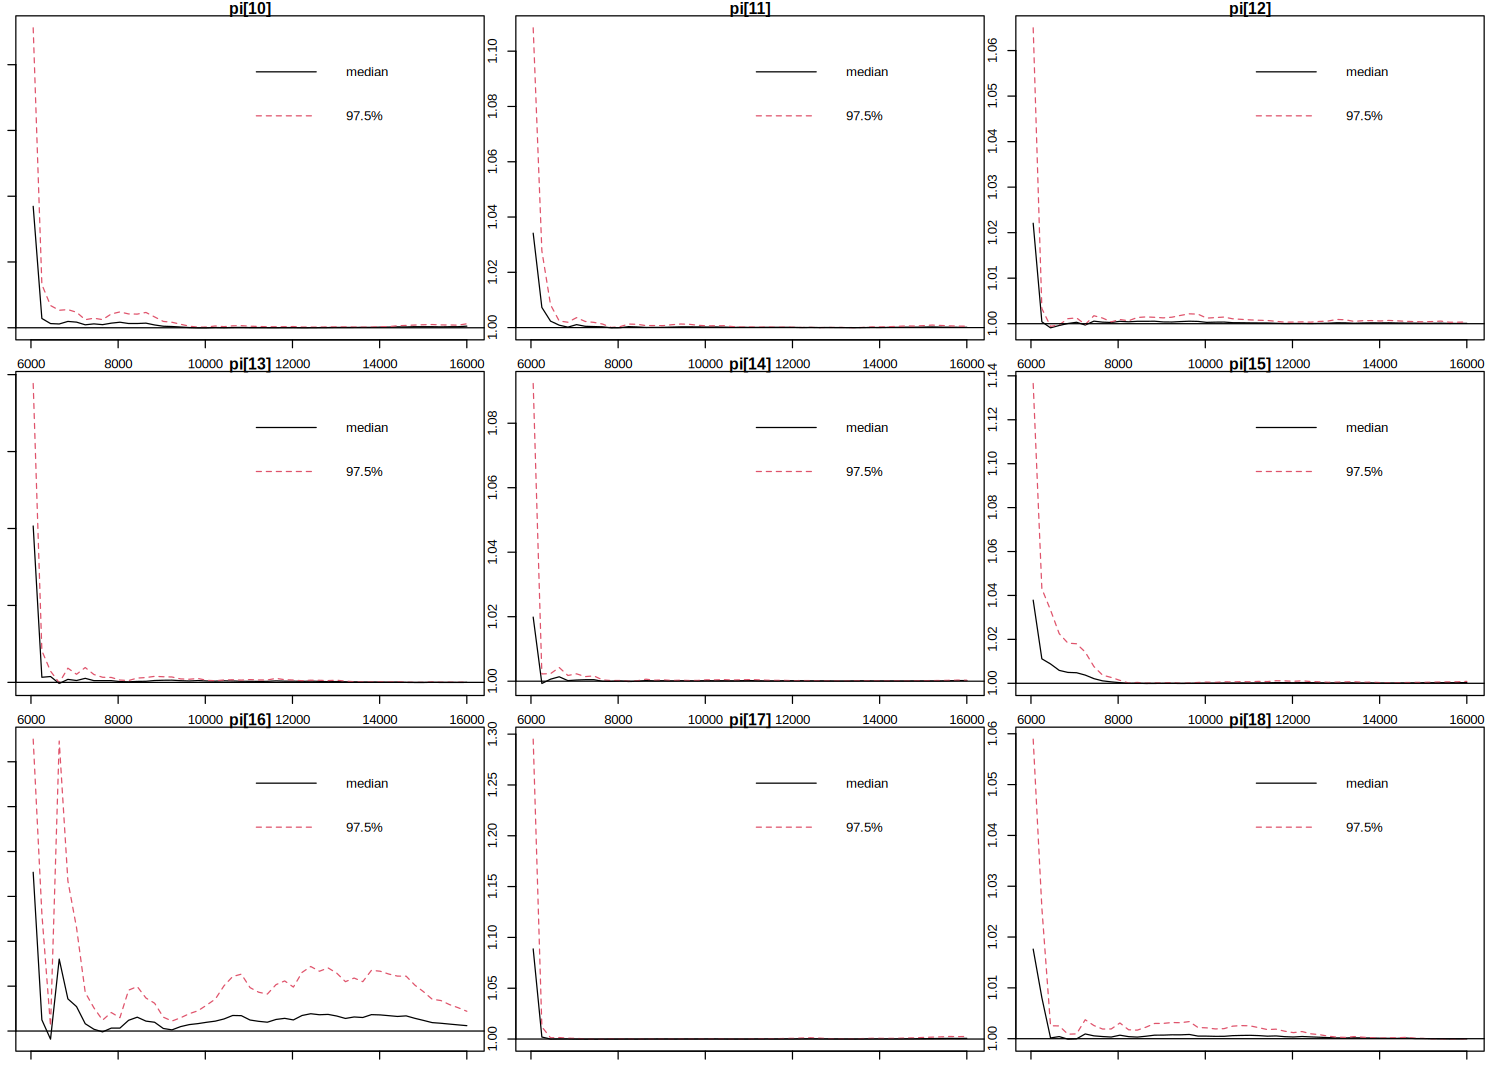
\includegraphics[width=\linewidth, height=8cm]{pictures/GRB2.png}
        %\caption{pi[21:40]}
        %\label{fig:sub1_2}
    \end{subfigure}
    
    \caption{Sample Gelman-Rubin-Brooks plots for $\pi_i$}
    \label{fig:GRBm1}
\end{figure}
\FloatBarrier % Ensures the figure doesn't float past this point

\textbf{Heidelberger–Welch (HW) diagnostic}: The Heidelberger–Welch tests, that is, stationarity test as well as the halfiwidth test were passed for almost all $\pi_i$ except a few in the first chain. Further iterations did not make any change.

\textbf{Raftery–Lewis (RL) diagnostic}: The dependence factor for deviance was 0.881 and for all $\pi_i$ was below 2 indicating independent sampling therefore signalling good convergence. Only a dependence factor of greater than 5 would indicate convergence issues.


\subsubsection{What do you conclude from this model?}

% Convergence was good in this model as per the diagnostics tests and also with stationarity for all $\pi_i$ achieved almost instantly as indicated by the graphical tests. 
% The mean posterior participation rates are shown in table \ref{tab:params1} and \ref{tab:params2} (appendix). Generally, municipalities with a high observed participation rate also have a high posterior participation rate and vice versa. There is considerable variation in the posterior distributions of $\pi_i$ with the posterior mean participation rates ranging from 0.156 to 0.628. The municipalities with the highest and lowest mean posterior participation rate are of Boechout (0.628, sd=0.012) and Drogenbos (0.156, sd=0.015). The majority of the municipalities, that is 171 ($\approx 60\%$) have a mean posterior participation rate of $\geq$ 0.5. Five (5) municipalities have a mean posterior participation rate of $<0.25$. Including Drogenbos, these are Kraainem, Linkebeek, Sint-Genesius-Rode and Wemmel.

Model 1 takes into account that participation rates differ across municipalities. This would suffice if there was need for targetted intervention at municipal level. The model as specified, however, does not explicitly estimate the difference in participation rates for age and gender by not accounting for associated cluster effects. 

Overall, the model demonstrated good convergence as indicated by graphical diagnostics, including traceplots, autocorrelation plots, and running mean plots, as well as formal diagnostic tests such as the Geweke diagnostic, Brooks-Gelman-Rubin (BGR) statistic, Heidelberger-Welch diagnostic, and Raftery-Lewis diagnostic.  Stationarity for all  $\pi_i$'s was achieved almost immediately, as confirmed by graphical assessments.

The mean posterior participation rates are presented in Tables \ref{tab:params1} and \ref{tab:params2} (Appendix). We also notice that generally, municipalities exhibiting high observed participation rates also demonstrate high posterior participation rates, and vice versa. Since we used non-informative priors for the participation rate $\pi_i$, the posterior $\pi_i$'s are dominated by the data. 

The overall trend highlights huge variation in the posterior participation rates across the regions. The posterior $\pi_i$ ranges from 0.156 to 0.628. Boechout has the highest mean posterior participation rate (0.628, SD = 0.012), while Drogenbos has the lowest (0.156, SD = 0.015). The majority of municipalities (171, approximately 60\%) have a mean posterior participation rate of 0.5 or greater. Careful review of this variation may offer actionable insights for targetted interventions. This may benefit regions with relatively low participation rates such Drogenbos, Kraainem, Linkebeek, Sint-Genesius-Rode, and Wemmel whose posterior mean participation rate falls below 0.25.


\subsubsection{Present a caterpillar plot of the posterior participation rates.}

As a sample, the caterpillar plot of the posterior estimates $\Bar{\pi_i}$ with the respective 95\% equal-tail credible interval for the first 20 municipalities ($\pi$[1-20]) are shown in figure \ref{fig:caterpillar1-20}. The points in the plot indicate the most likely participation rate ($\pi_i$) given the data and prior beliefs while the horizontal lines show the 95\% credible interval (CI) for $\pi_i$. The overlapping CIs, eg region 17,18 and 19 indicate that the posterior means are not clearly distinguishable given the data and prior information. The CIs for these regions don't overlap with that of region 20 suggesting that meaningful differences in the participation rate. We also noticed that the municipality of Herstappe (CI not shown) has a relatively large CI of the posterior mean $\pi$ indicating high uncertainty. This uncertainty perhaps reflects the municipality's fairly low number of participating (3) and invited (8) people. Note that we do not show the complete caterpillar plot as it was too cluttered due to many observations. 

\begin{figure}
    \centering
    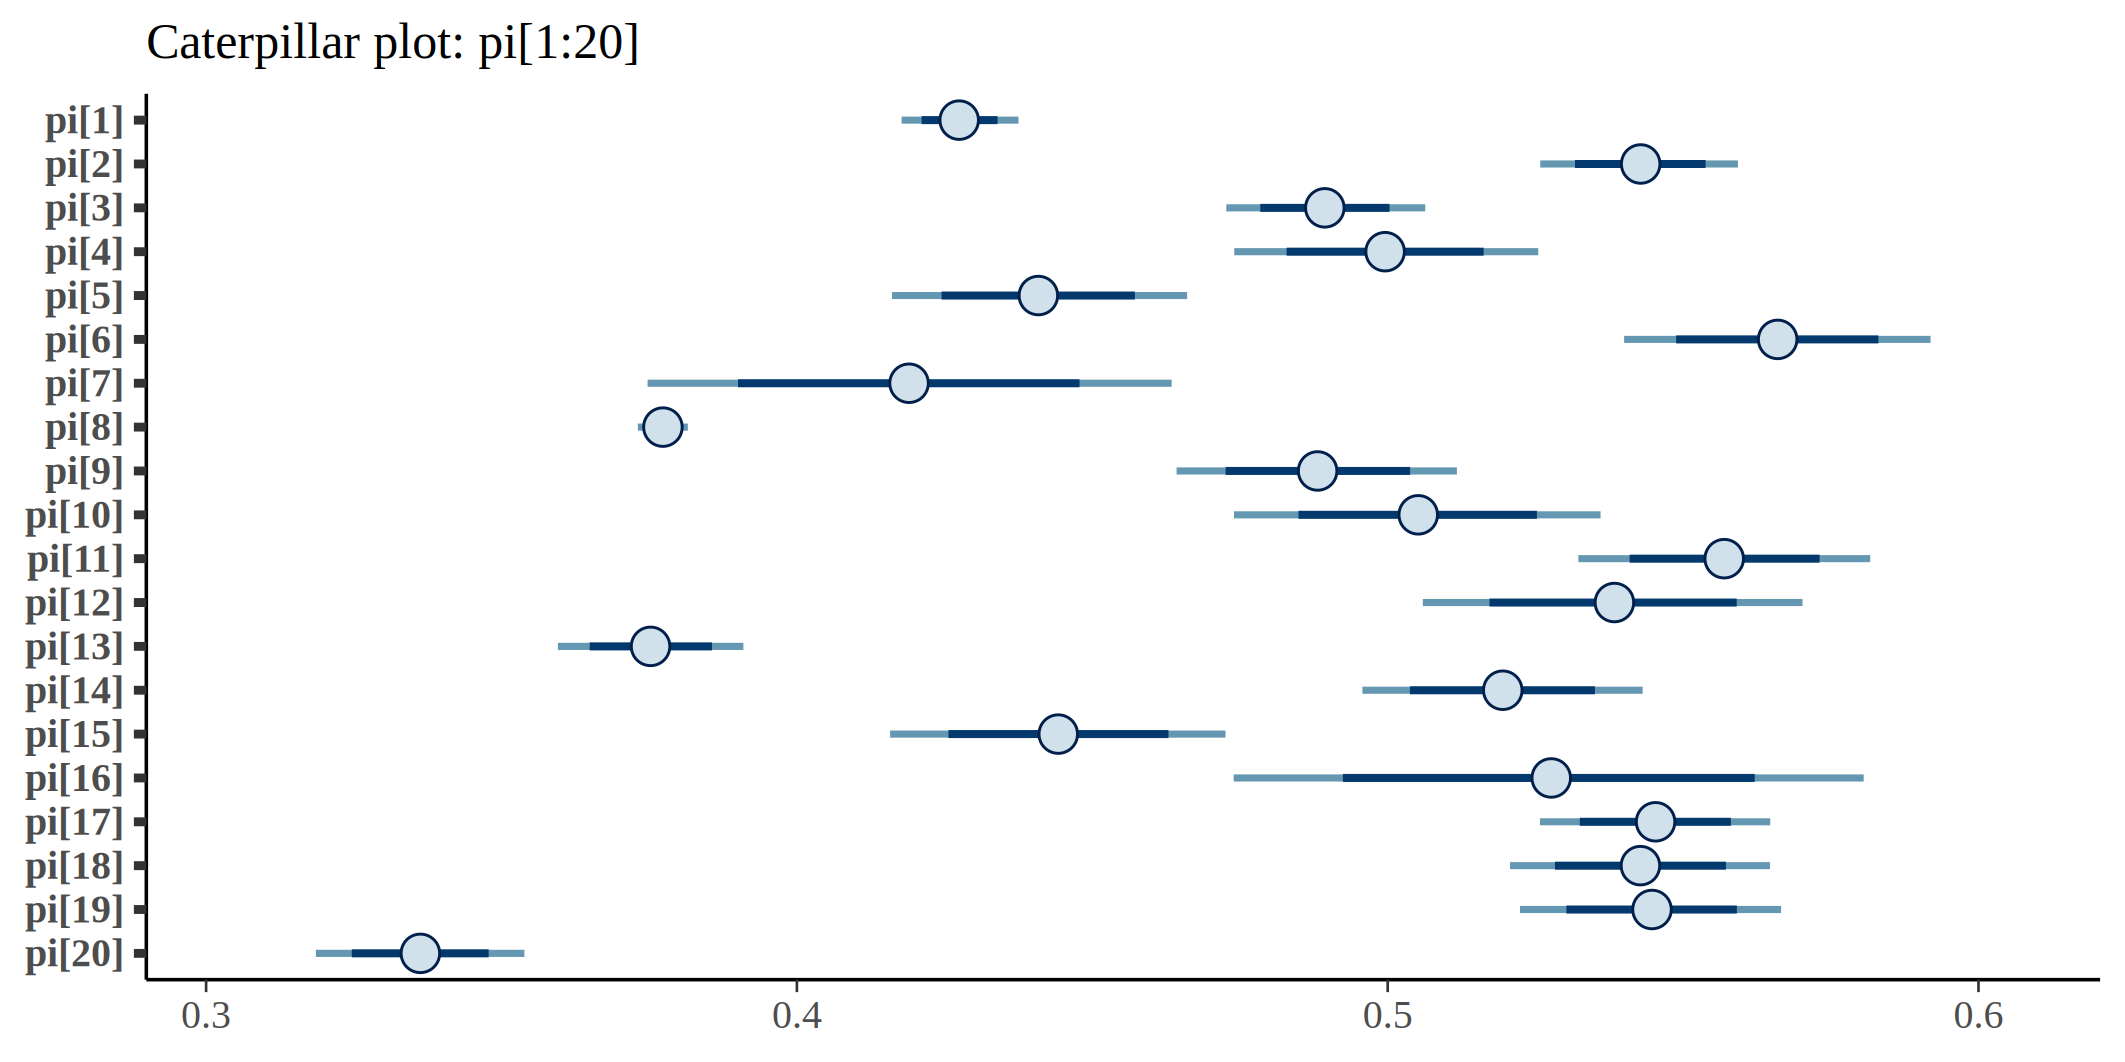
\includegraphics[width=0.75\linewidth]{pictures/cater1-20.png}
    \caption{Caterpillar plot for the first 20 municipalities.}
    \label{fig:caterpillar1-20}
\end{figure}
\FloatBarrier

% \begin{figure}[h!]
%     \centering
%     % First row
%     \begin{subfigure}{0.45\textwidth}
%         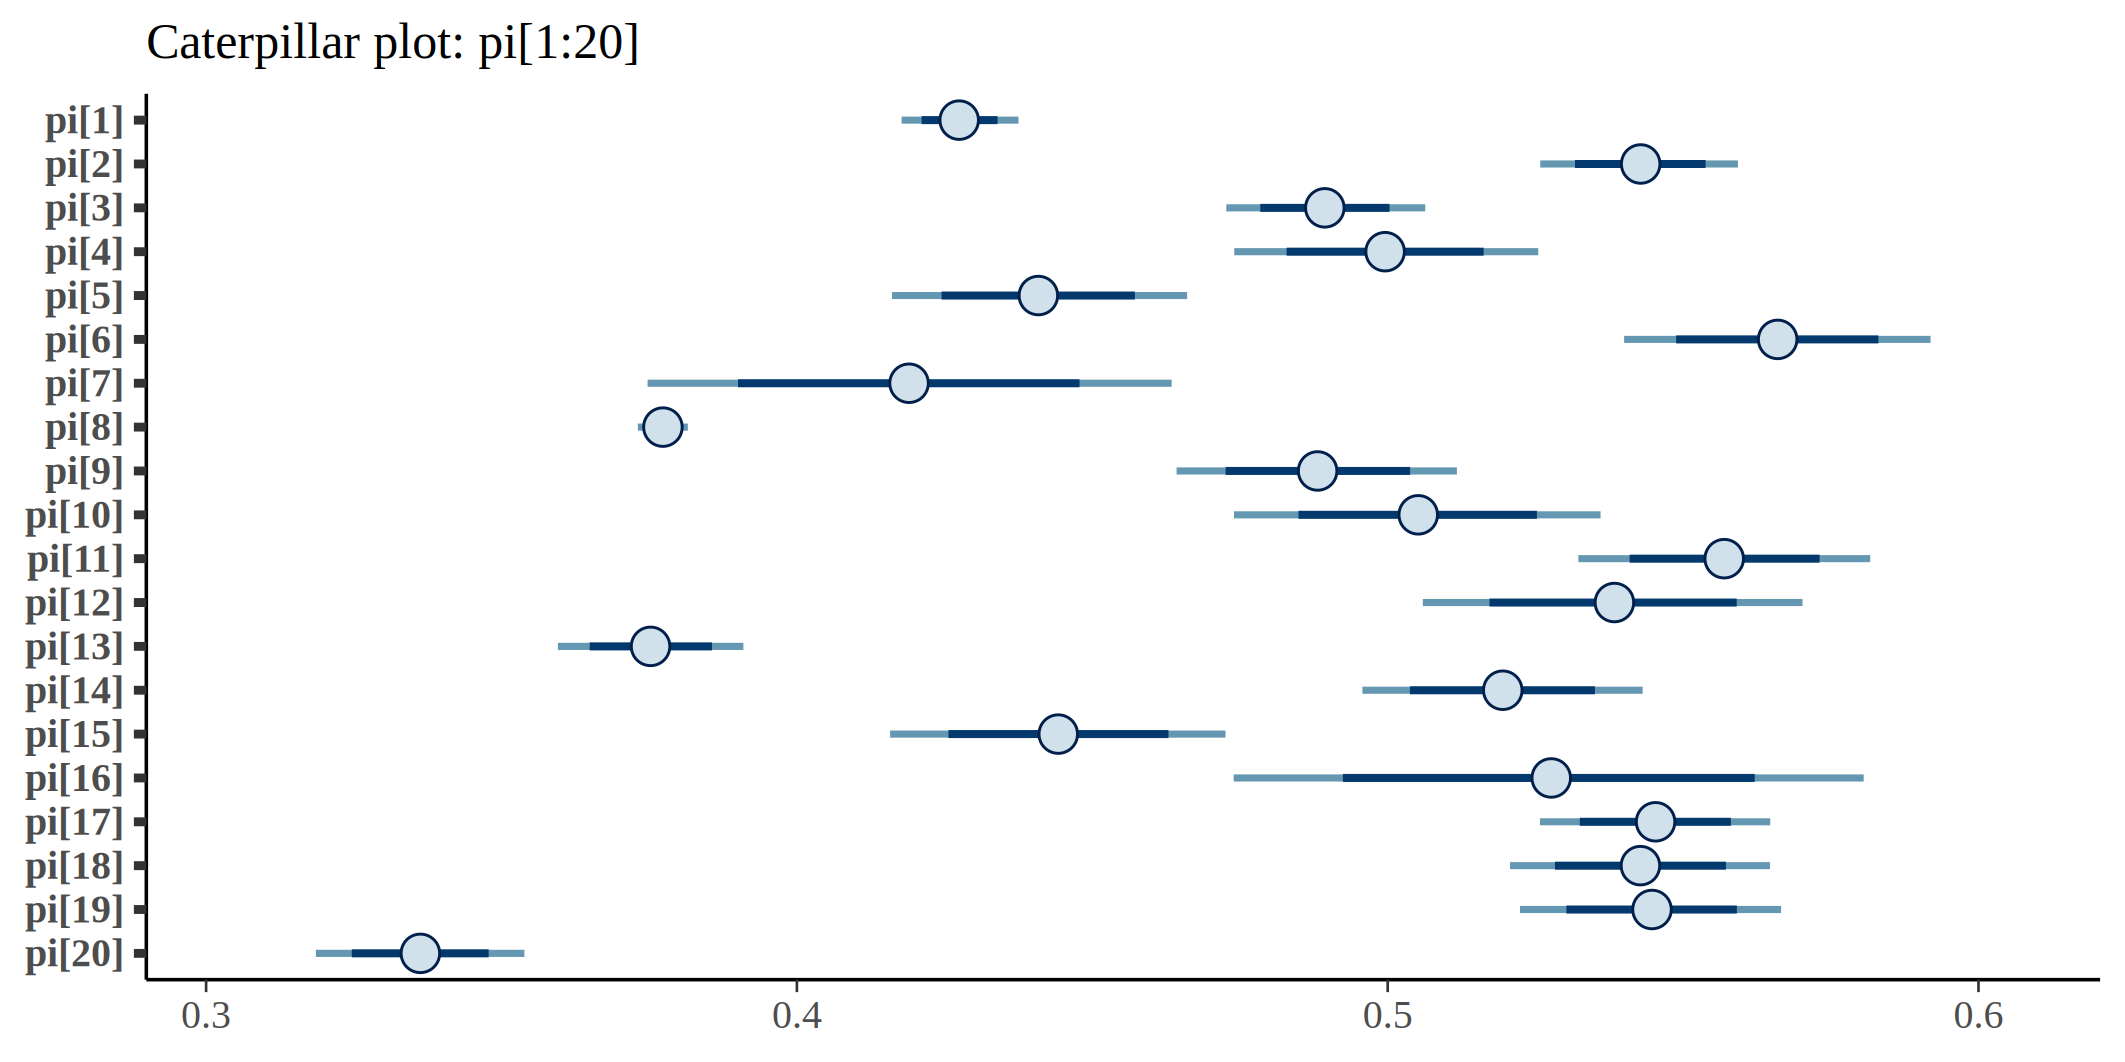
\includegraphics[width=\linewidth]{pictures/cater1-20.png}
%         \caption{pi[1:20]}
%         \label{fig:sub1_1}
%     \end{subfigure}
%     %\hfill
%     \begin{subfigure}{0.45\textwidth}
%         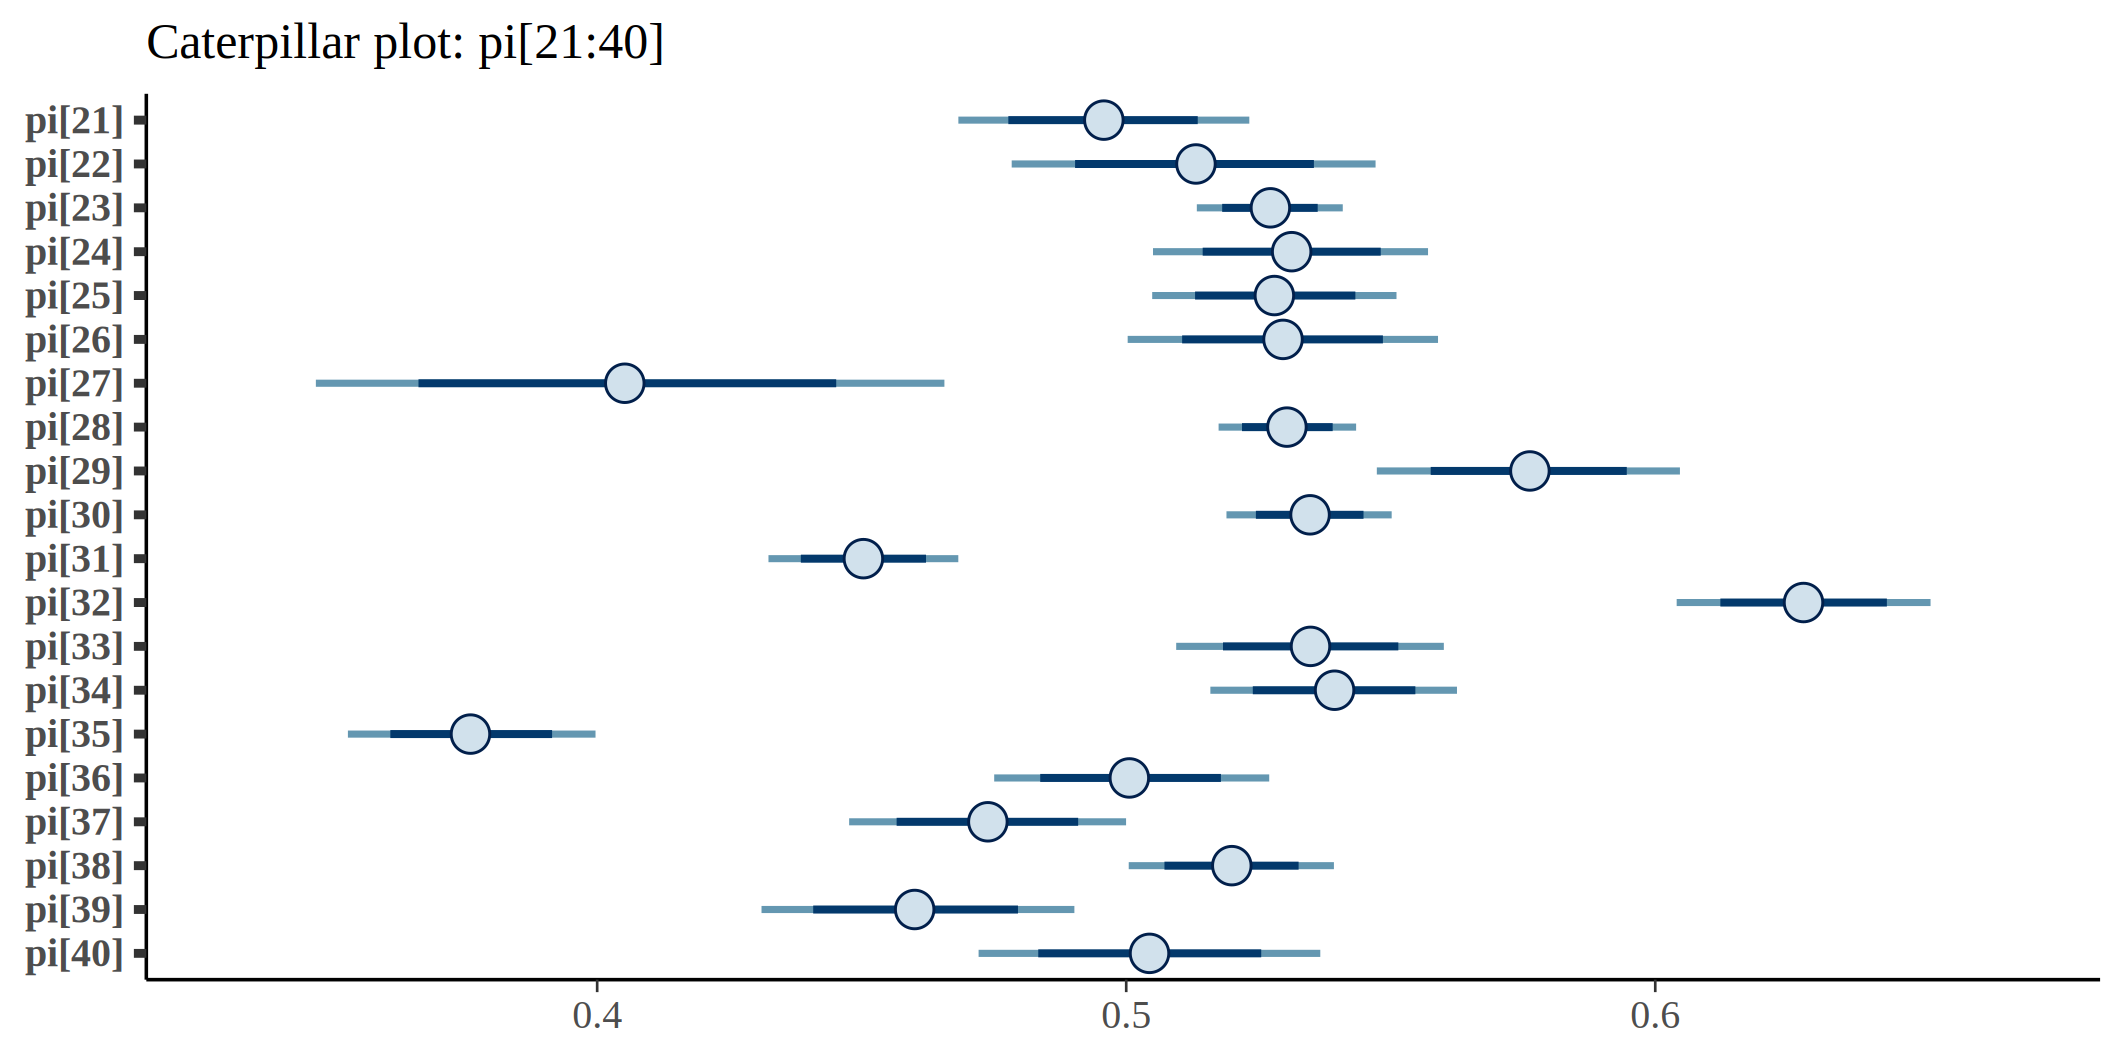
\includegraphics[width=\linewidth]{pictures/cater21-40.png}
%         \caption{pi[21:40]}
%         \label{fig:sub1_2}
%     \end{subfigure}

%     % Second row
%     \vskip\baselineskip
%     \begin{subfigure}{0.45\textwidth}
%         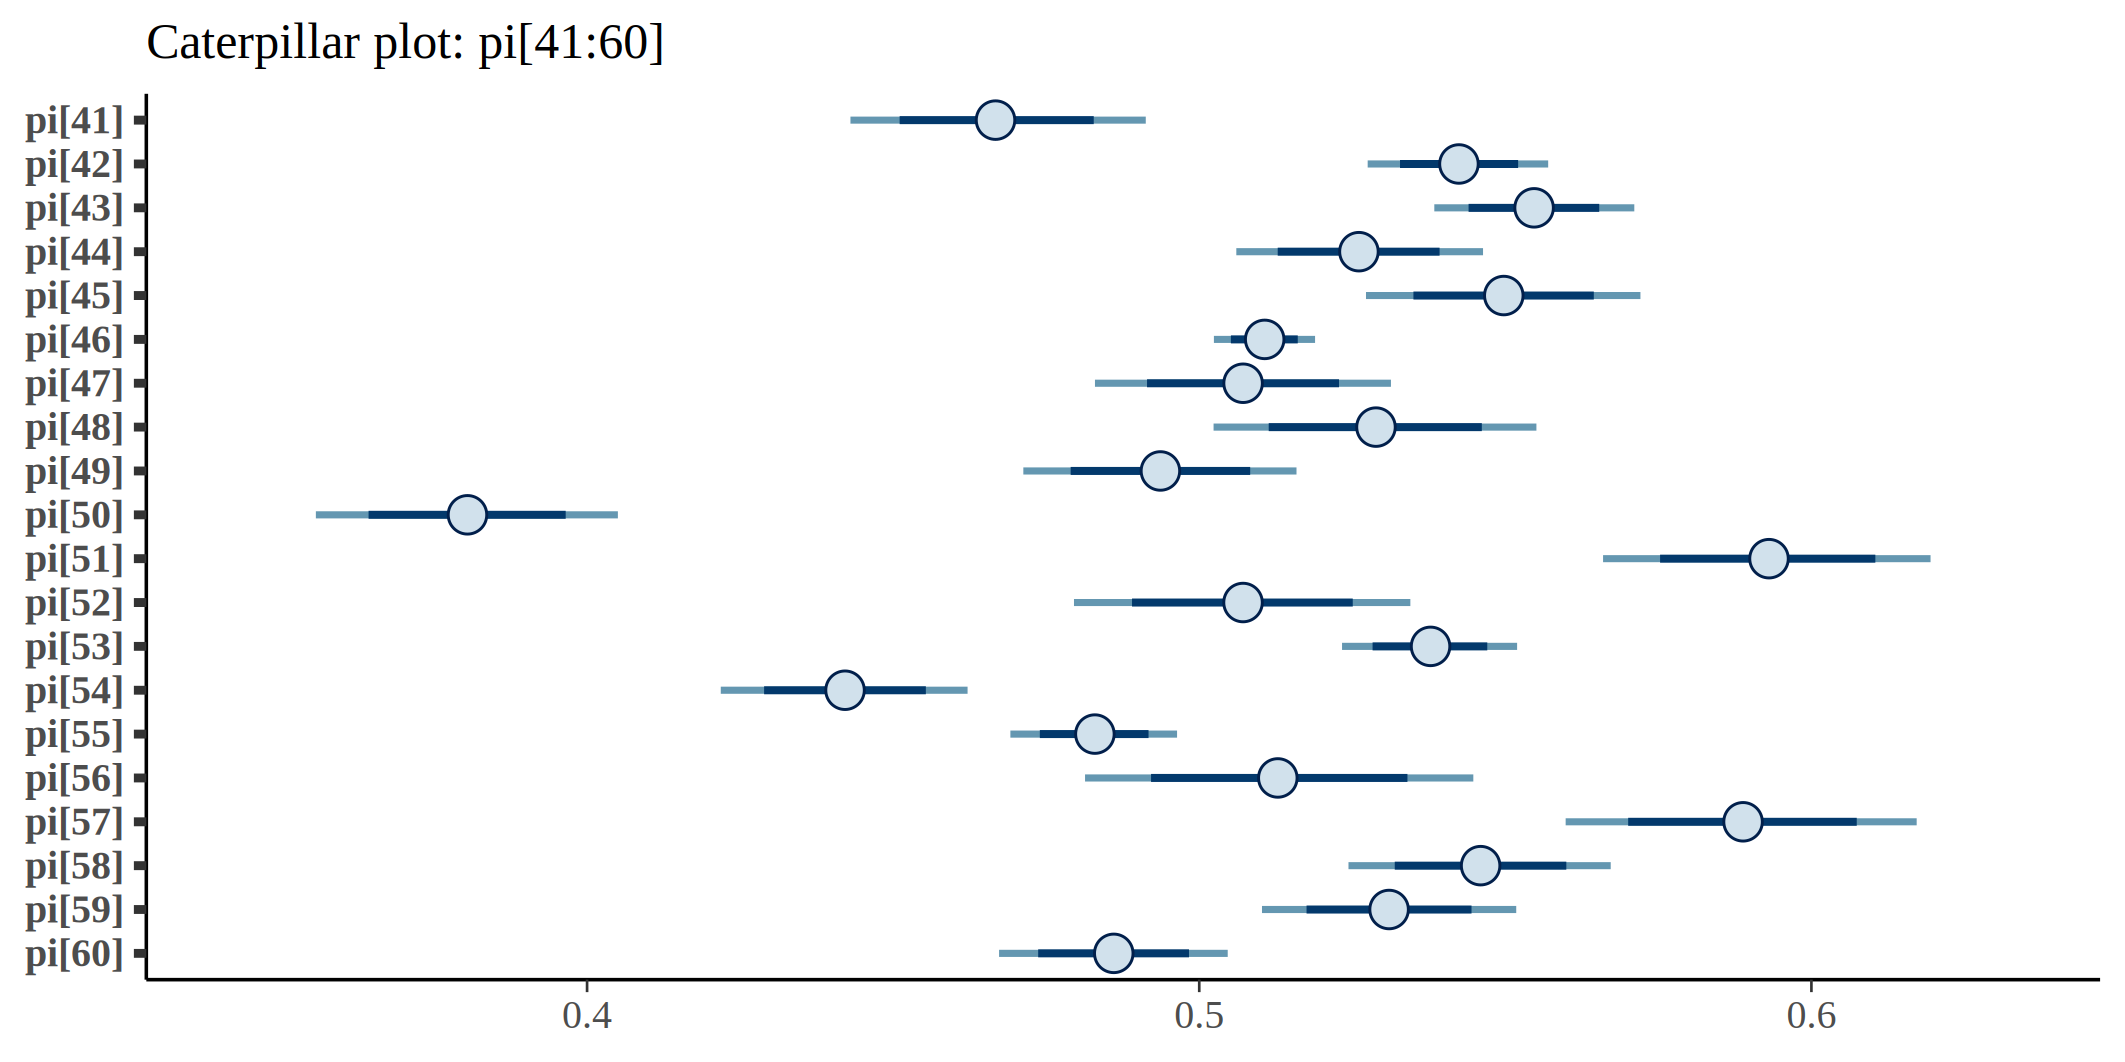
\includegraphics[width=\linewidth]{pictures/cater41-60.png}
%         \caption{pi[41:60]}
%         \label{fig:sub2_1}
%     \end{subfigure}
%     %\hfill
%     \begin{subfigure}{0.45\textwidth}
%         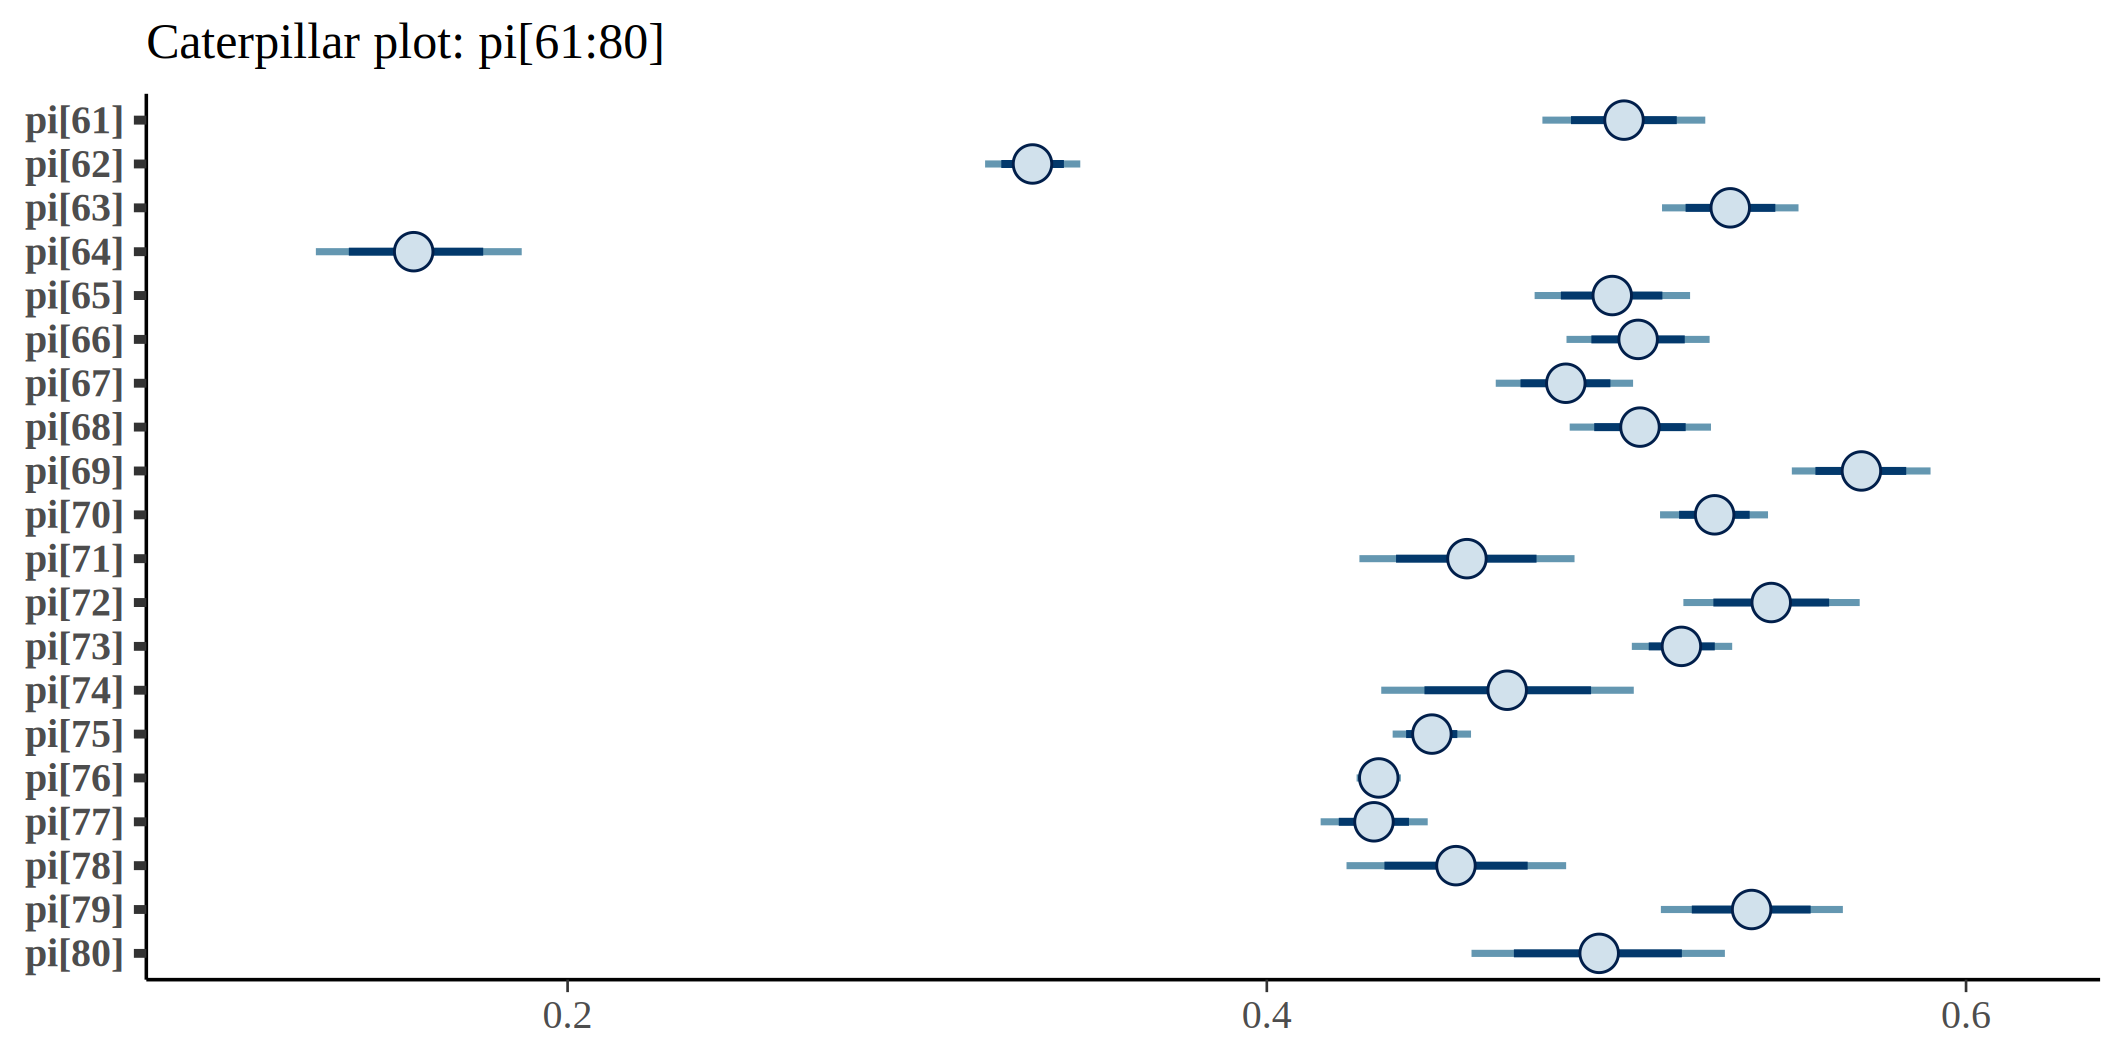
\includegraphics[width=\linewidth]{pictures/cater61-80.png}
%         \caption{pi[61:80]}
%         \label{fig:sub2_2}
%     \end{subfigure}

%     % third row
%     \vskip\baselineskip
%     \begin{subfigure}{0.45\textwidth}
%         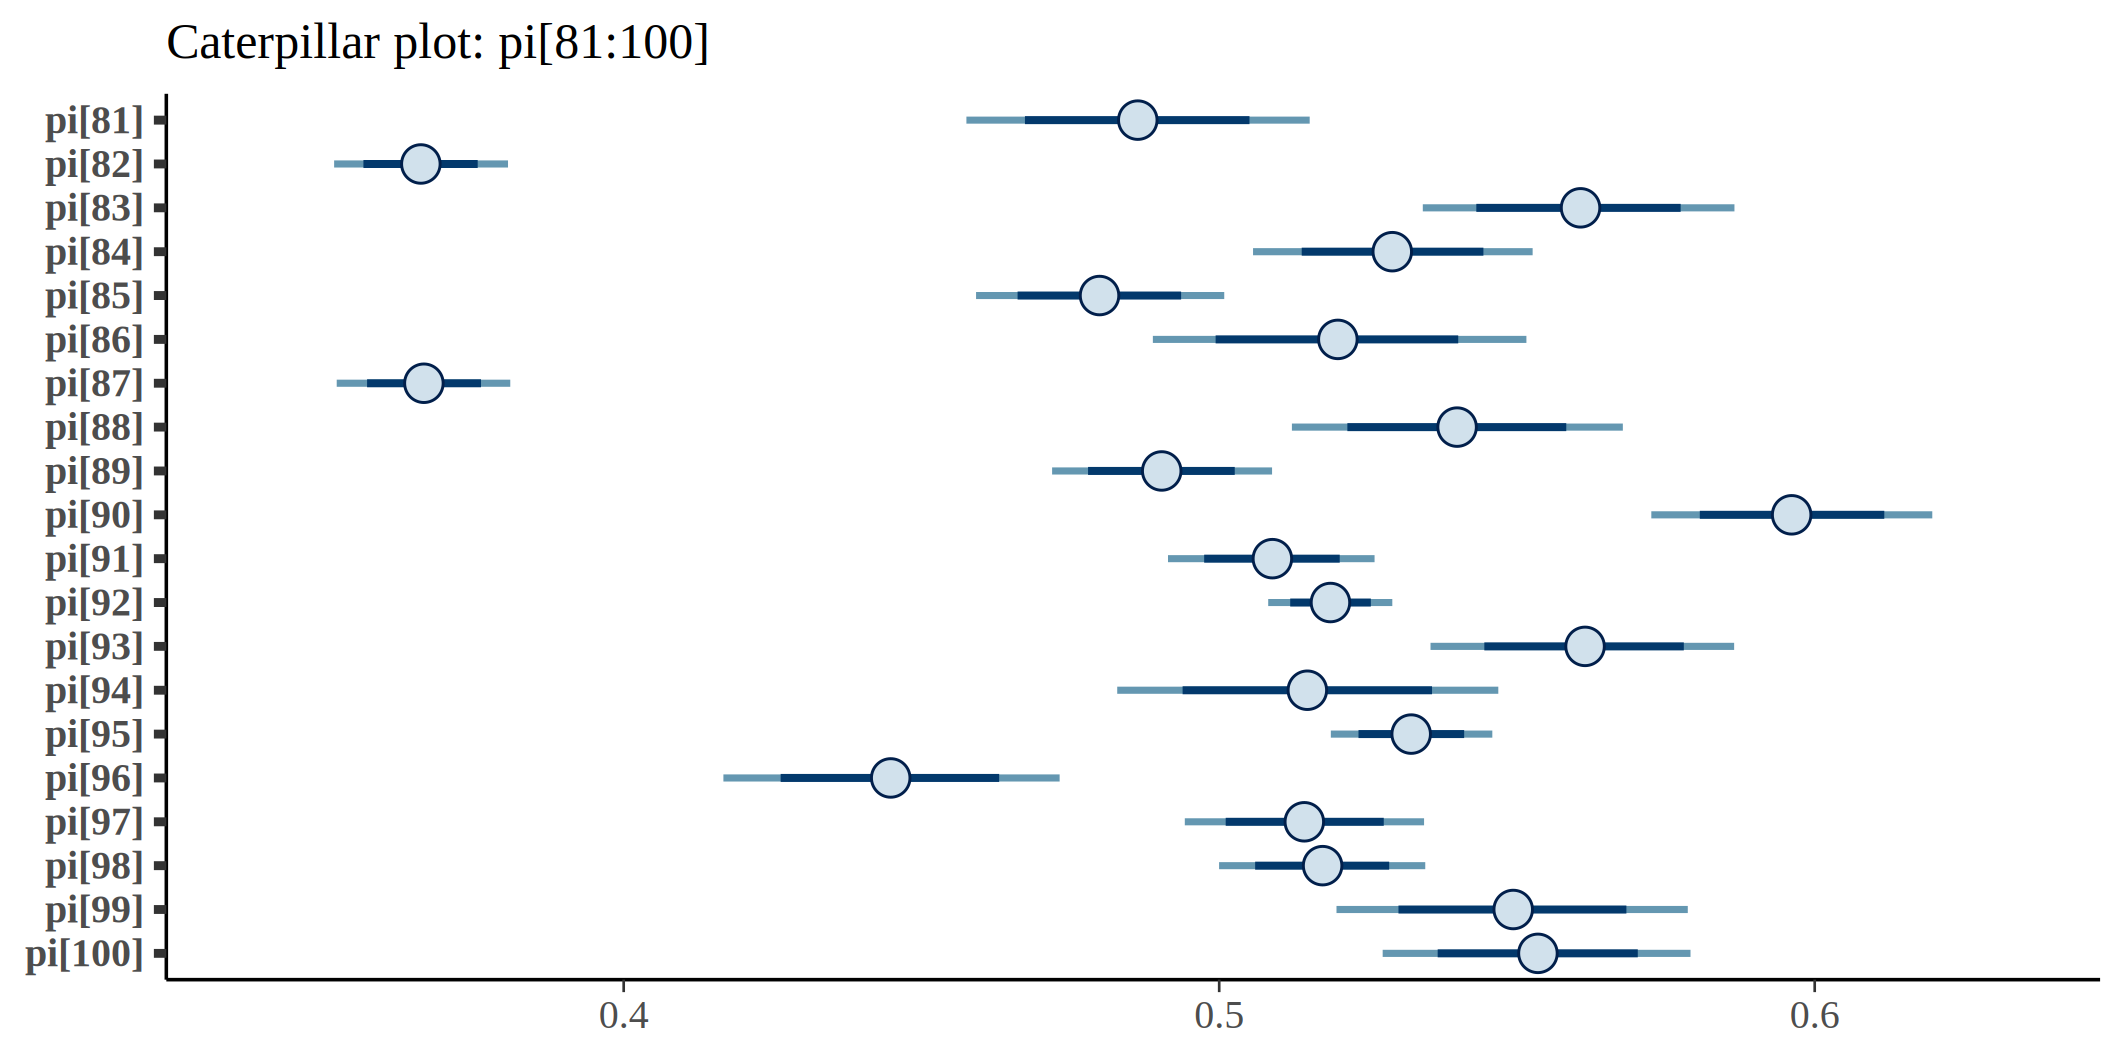
\includegraphics[width=\linewidth]{pictures/cater81-100.png}
%         \caption{pi[81:100]}
%         \label{fig:sub1_1}
%     \end{subfigure}
%     %\hfill
%     \begin{subfigure}{0.45\textwidth}
%         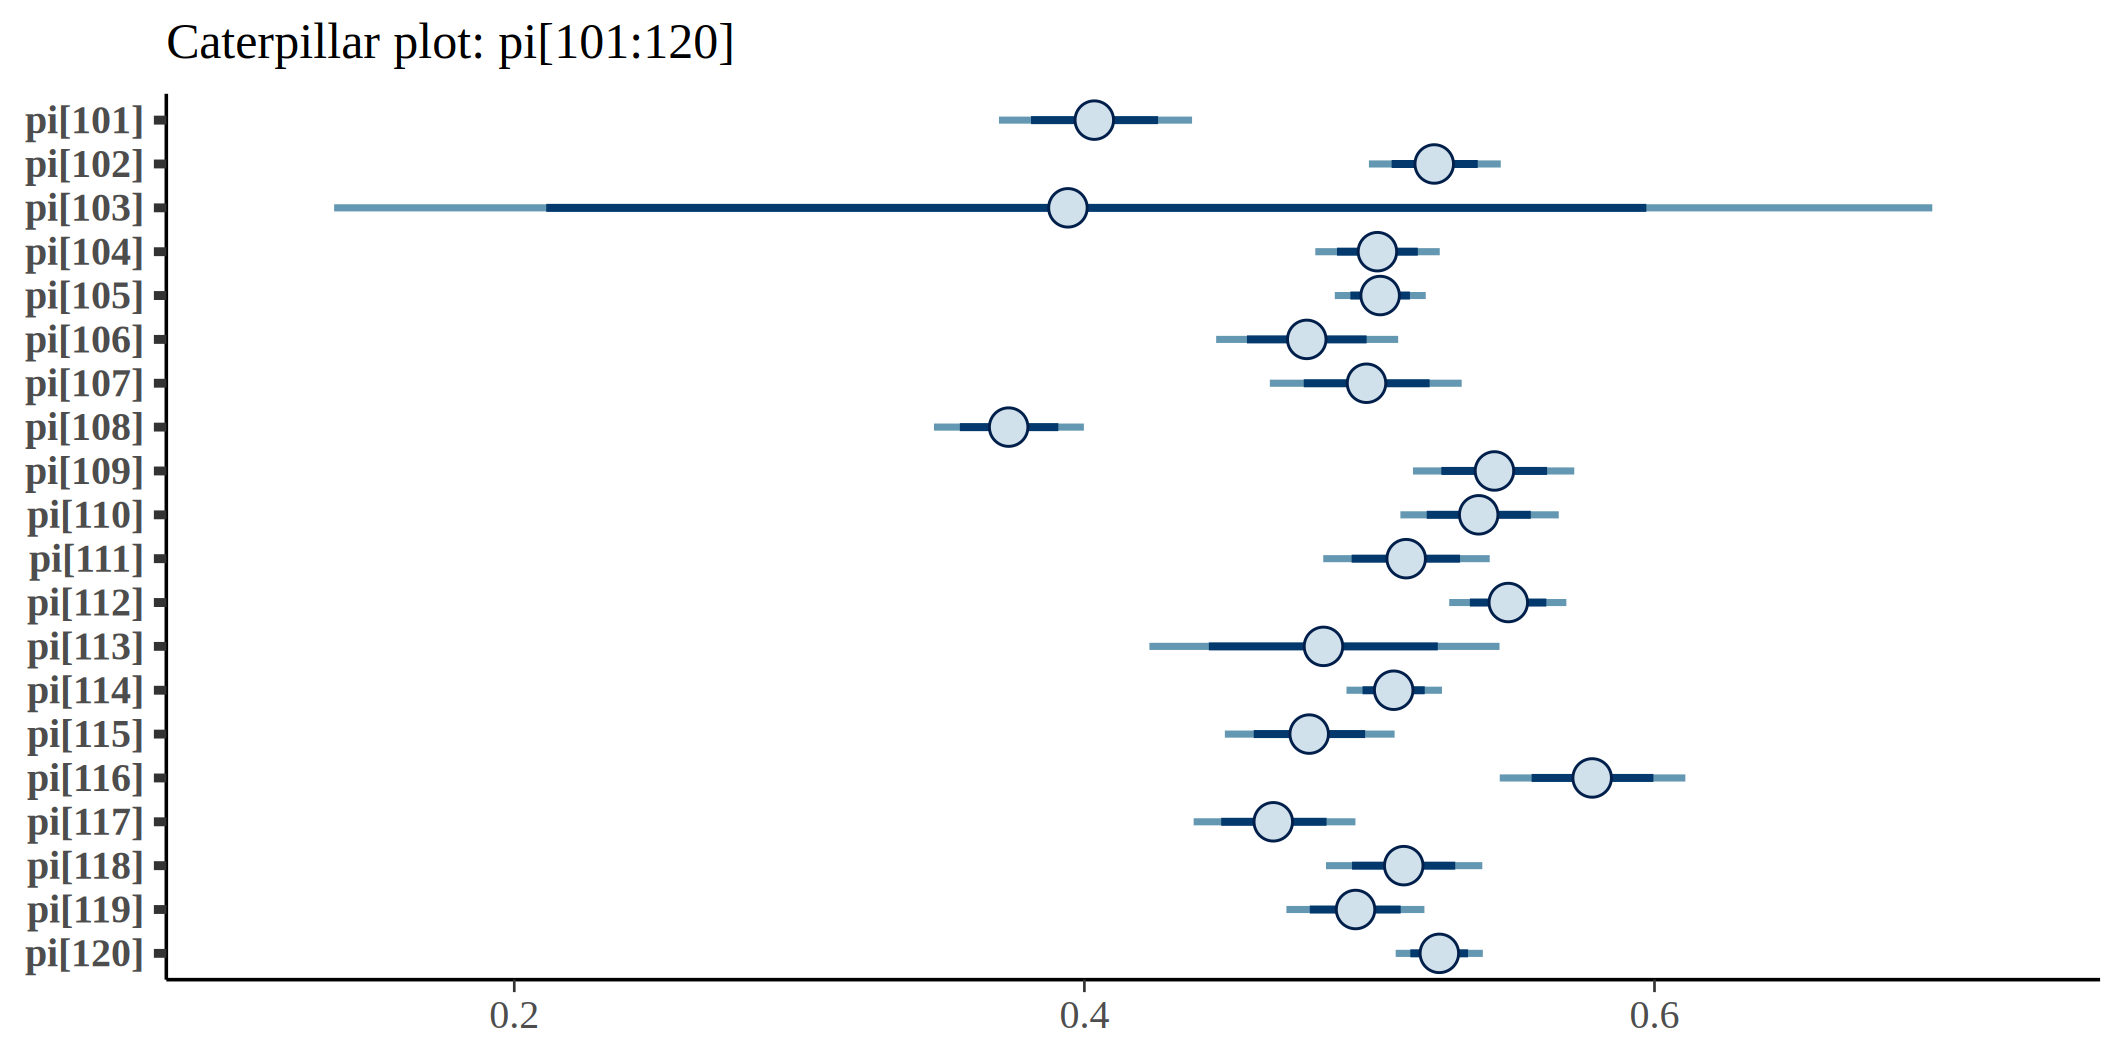
\includegraphics[width=\linewidth]{pictures/cater101-120.png}
%         \caption{pi[101:120]}
%         \label{fig:sub1_2}
%     \end{subfigure}
    
%     \caption{Posterior participation rates pi[1:120].}
%     \label{fig:caterpillar1-120}
% \end{figure}

% \begin{figure}[h!]
%     \centering
%     % First row
%     \begin{subfigure}{0.45\textwidth}
%         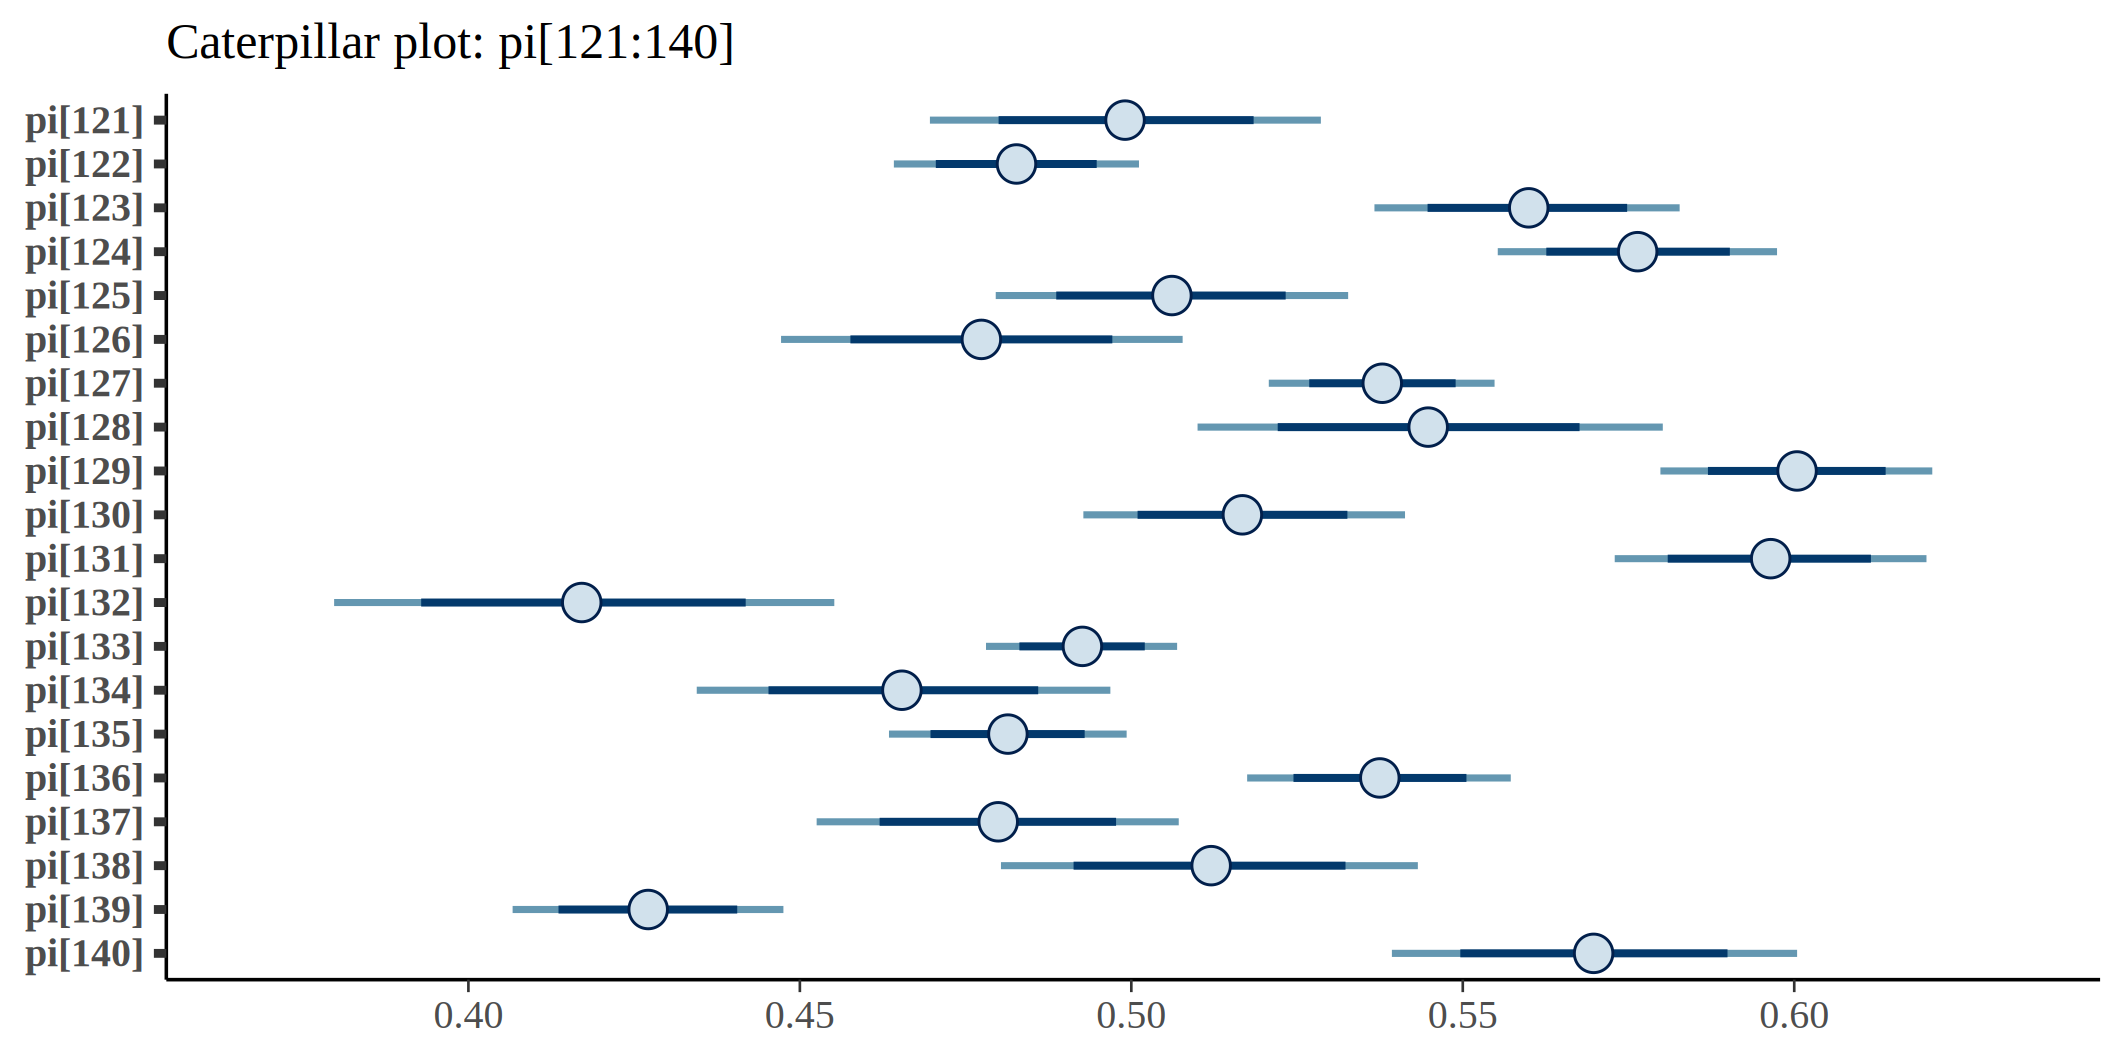
\includegraphics[width=\linewidth]{pictures/cater121-140.png}
%         \caption{pi[121:140]}
%         \label{fig:sub2_1}
%     \end{subfigure}
%     %\hfill
%     \begin{subfigure}{0.45\textwidth}
%         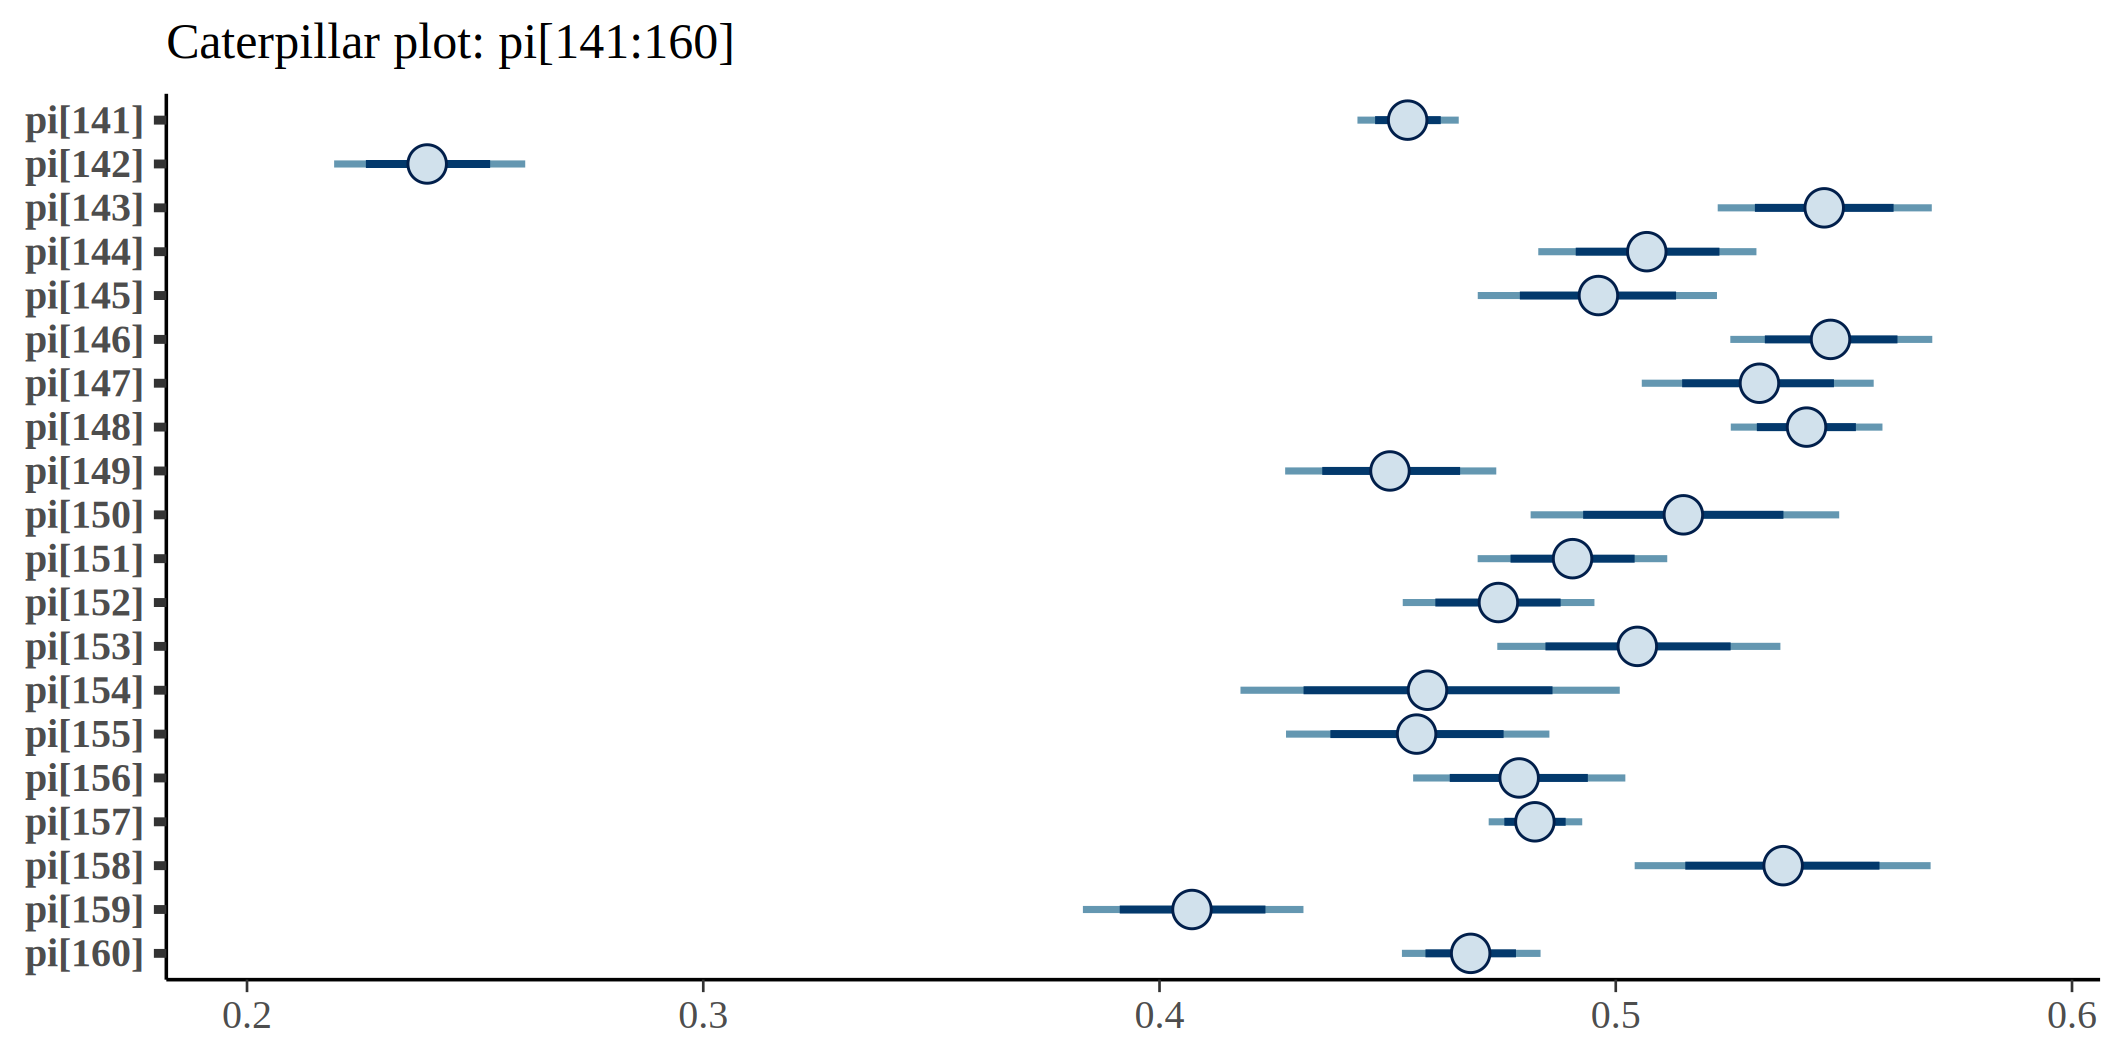
\includegraphics[width=\linewidth]{pictures/cater141-160.png}
%         \caption{pi[141:160]}
%         \label{fig:sub2_2}
%     \end{subfigure}

%     % second row
%     \vskip\baselineskip
%     \begin{subfigure}{0.45\textwidth}
%         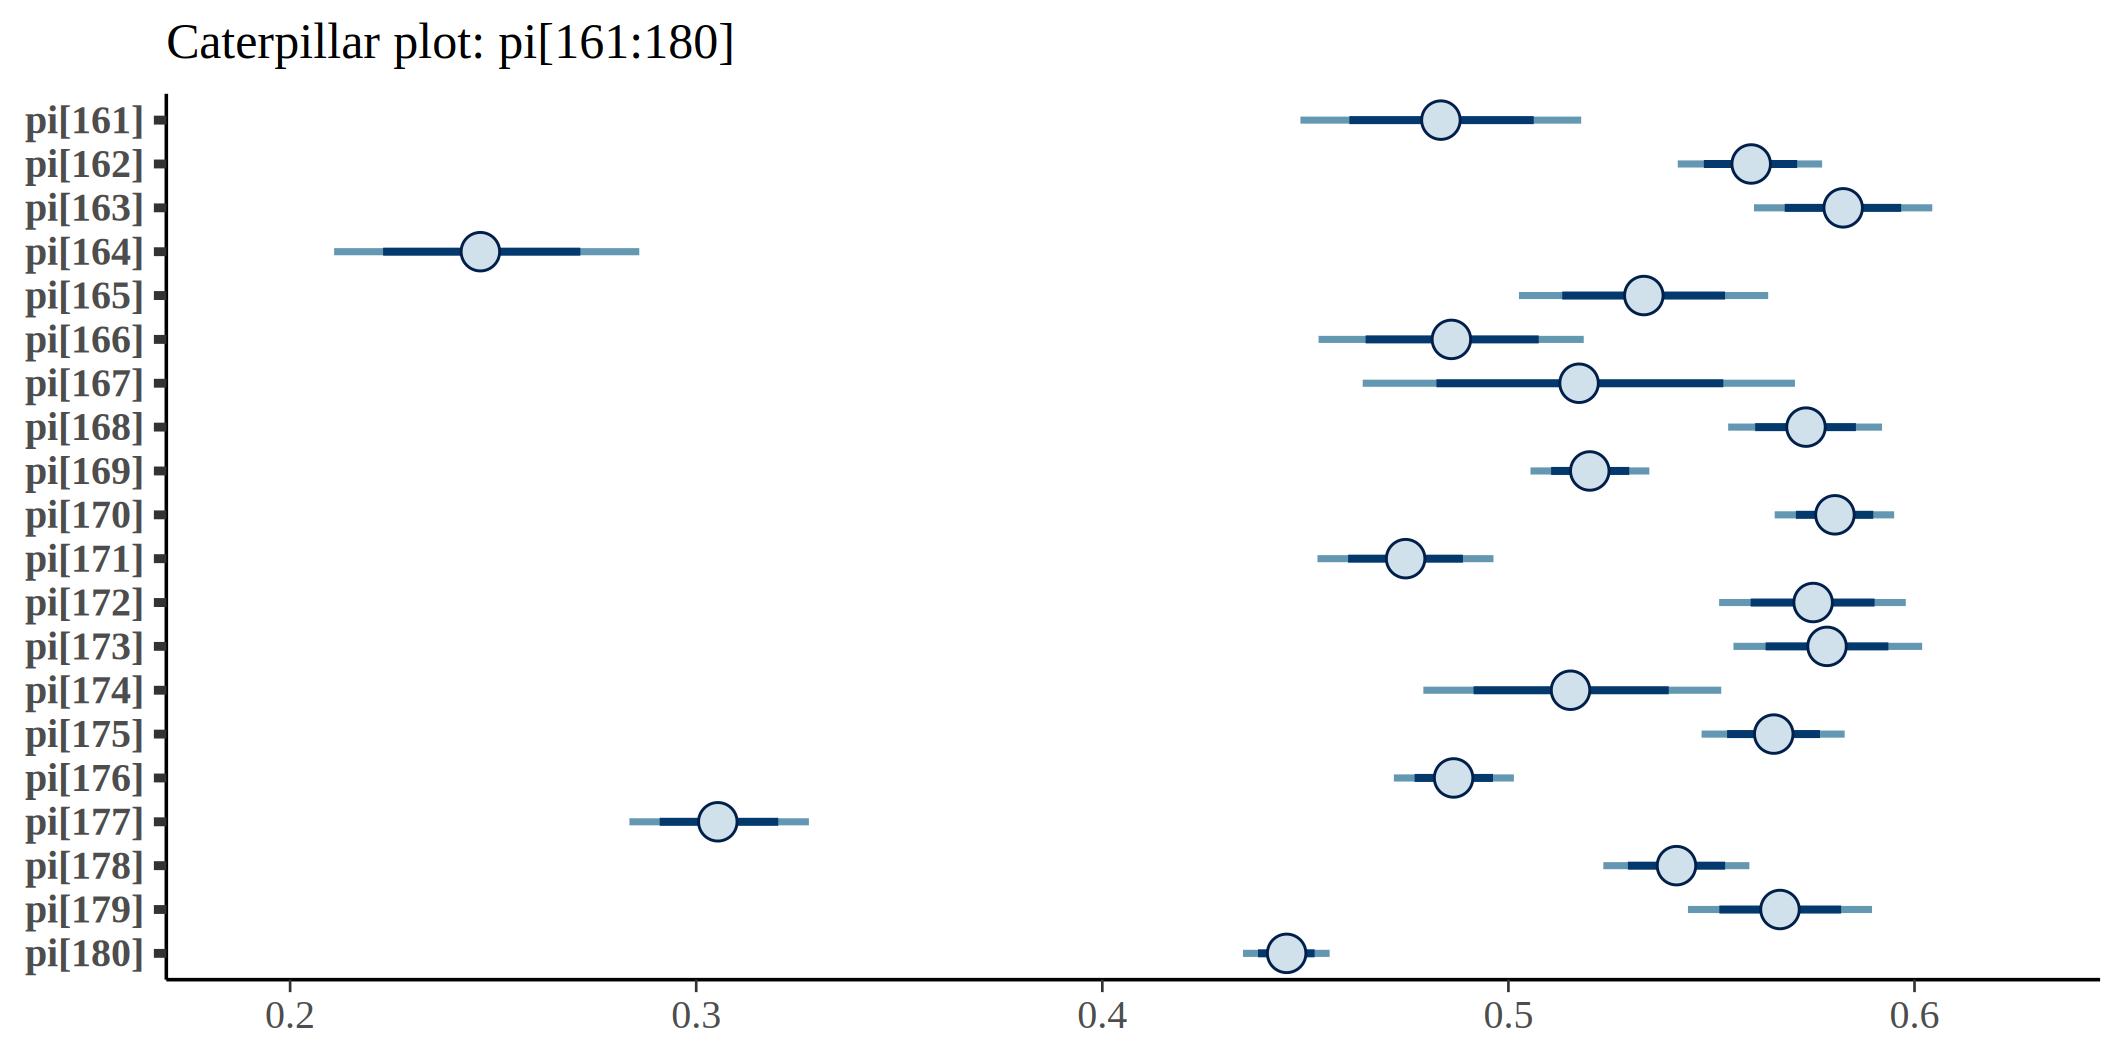
\includegraphics[width=\linewidth]{pictures/cater161-180.png}
%         \caption{pi[161:180]}
%         \label{fig:sub1_1}
%     \end{subfigure}
%     %\hfill
%     \begin{subfigure}{0.45\textwidth}
%         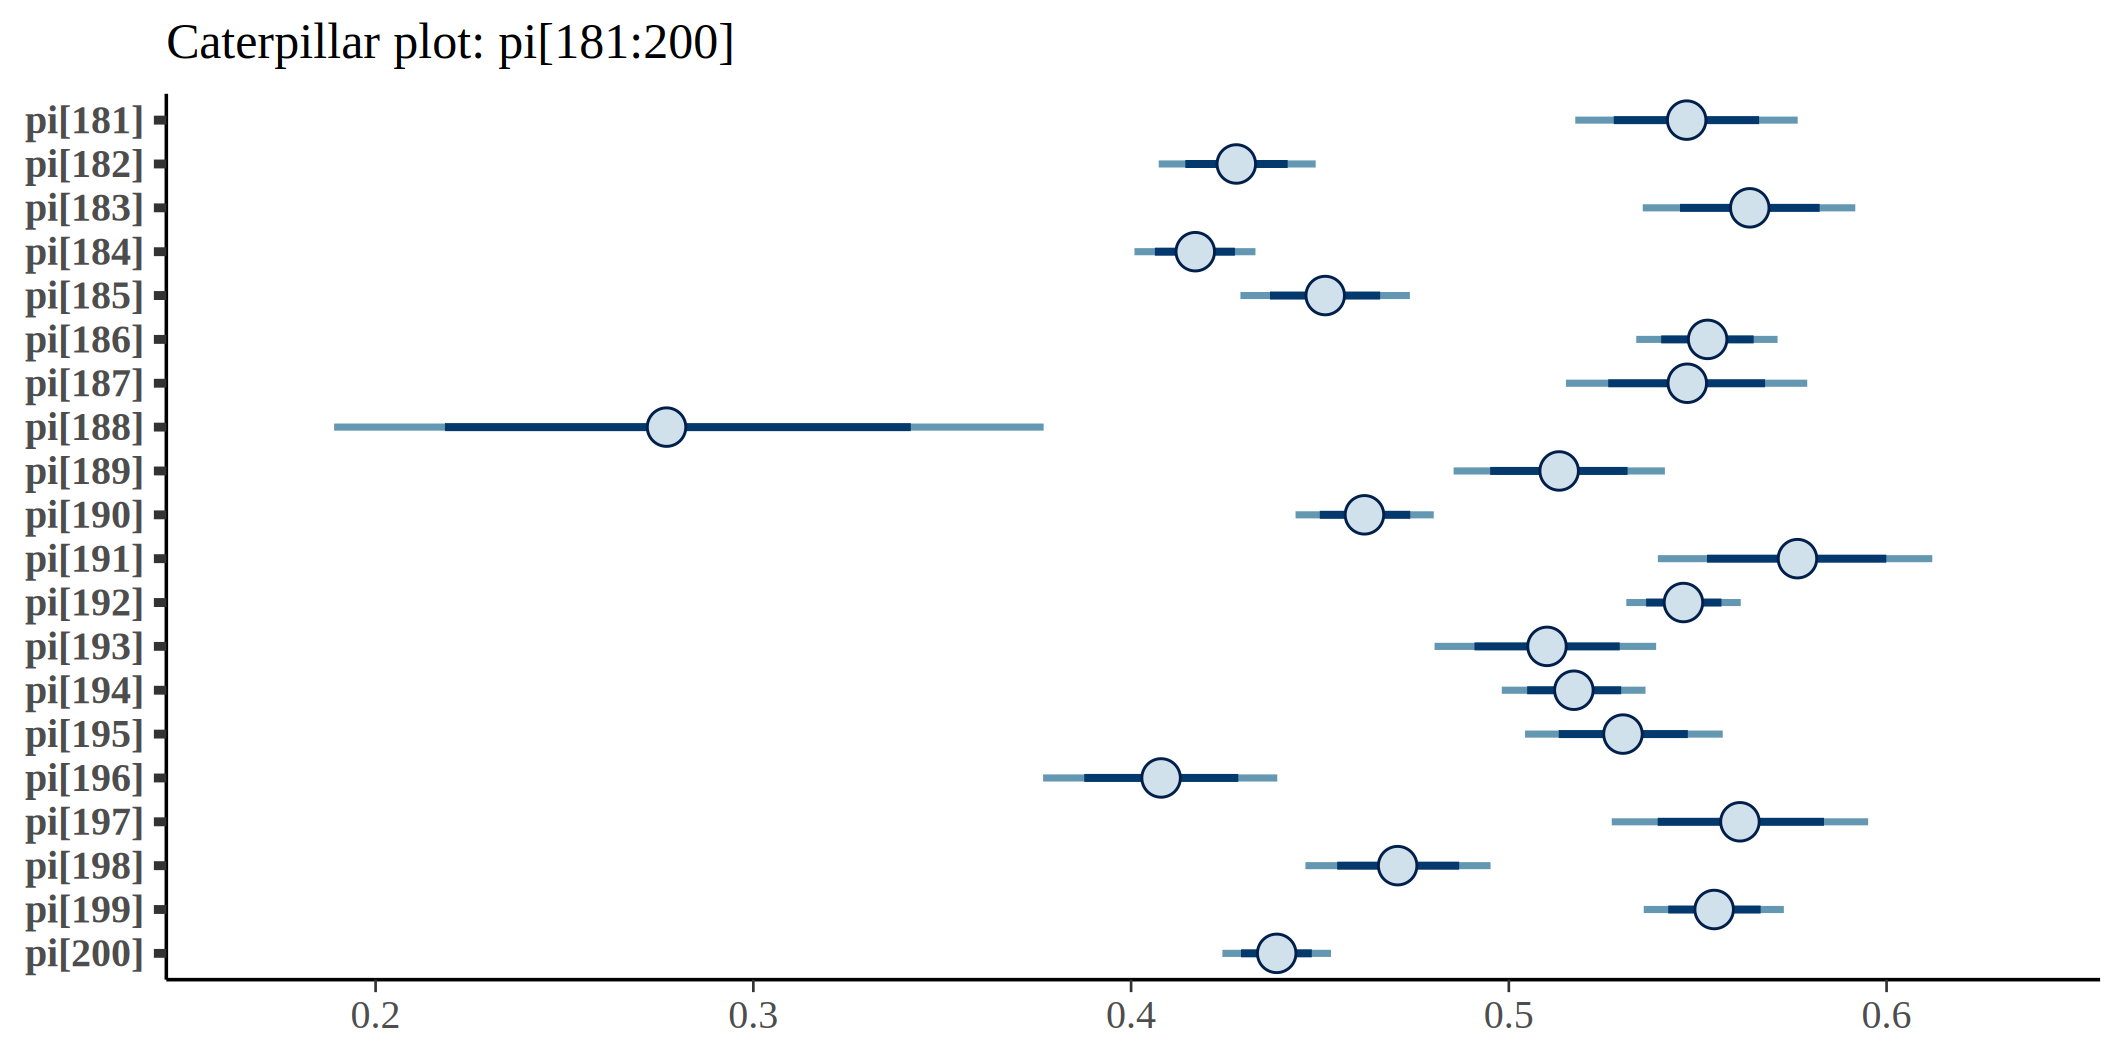
\includegraphics[width=\linewidth]{pictures/cater181-200.png}
%         \caption{pi[181:200]}
%         \label{fig:sub1_2}
%     \end{subfigure}

%     % third row
%     \vskip\baselineskip
%     \begin{subfigure}{0.45\textwidth}
%         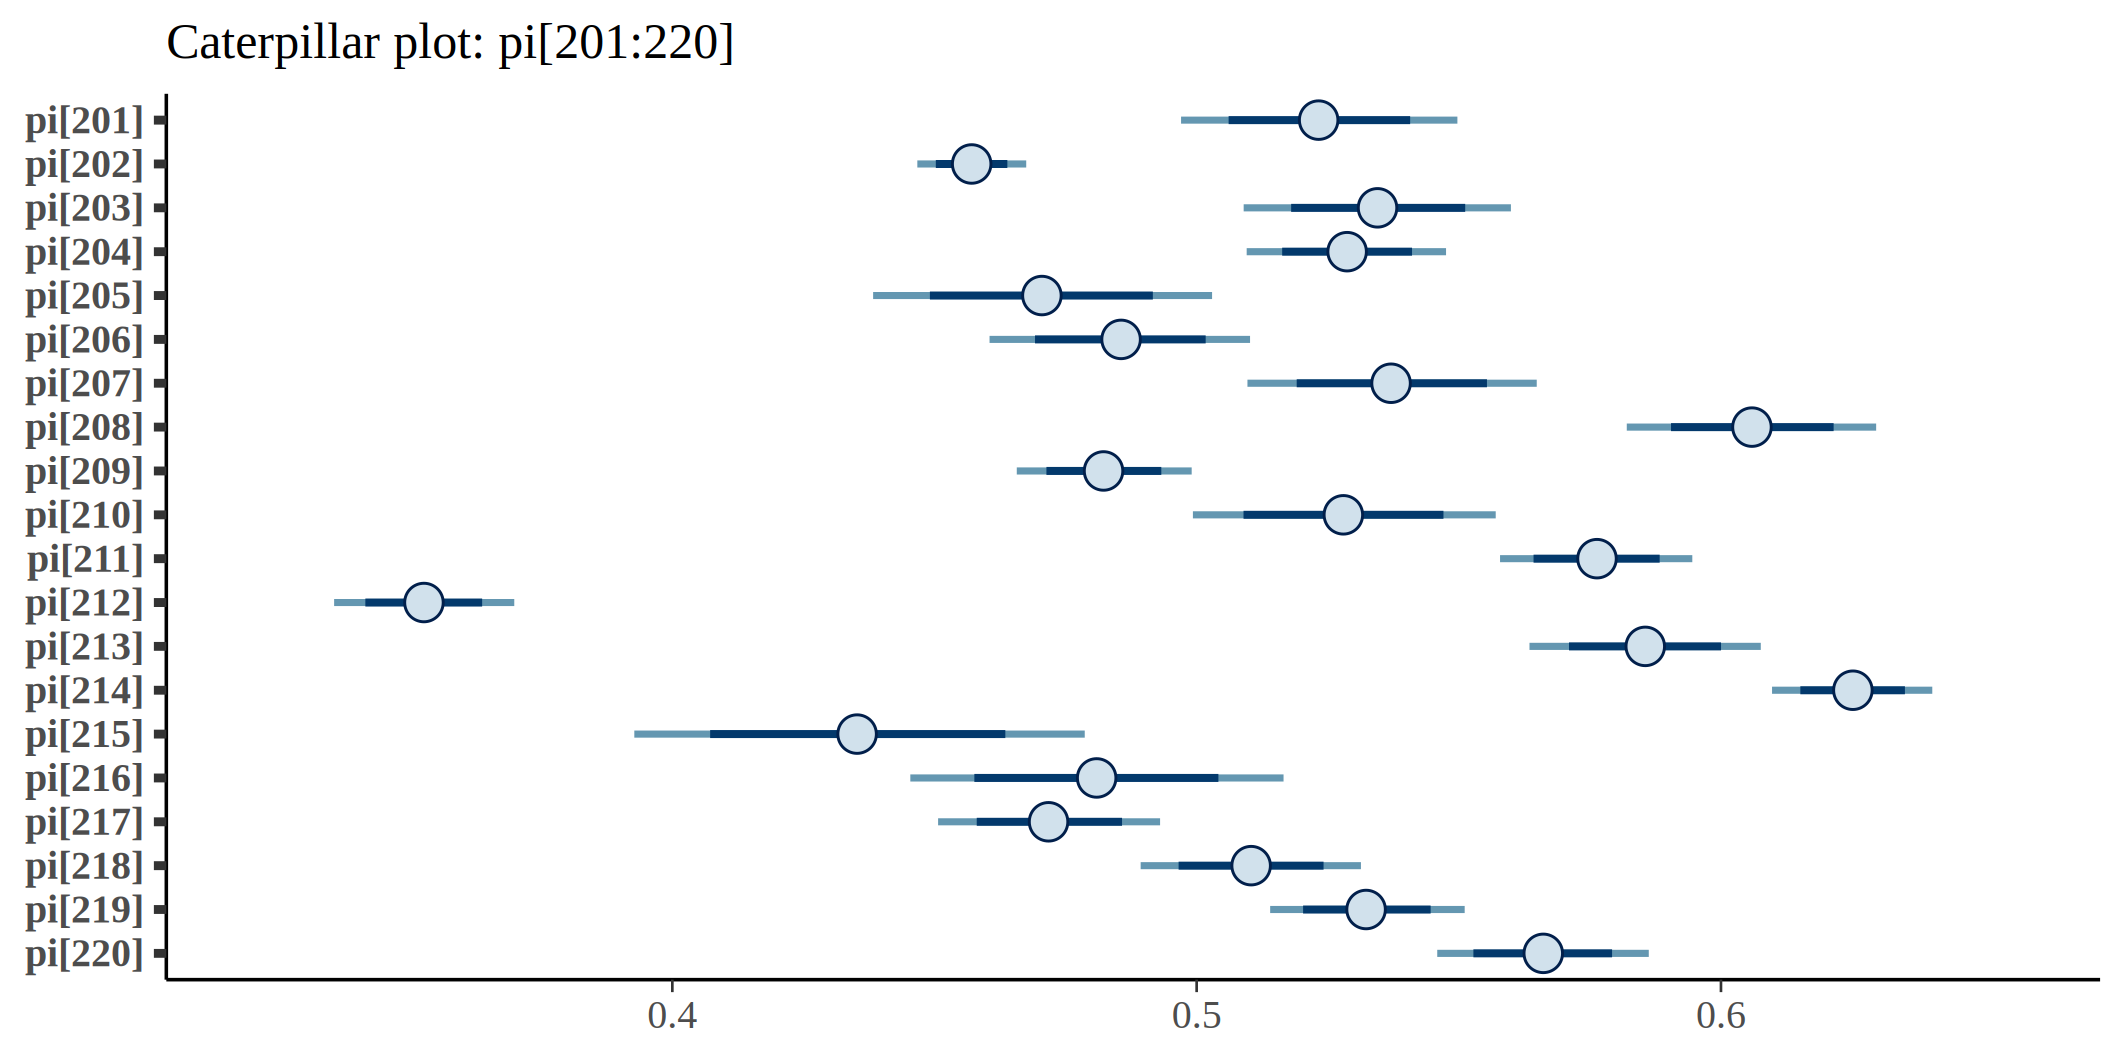
\includegraphics[width=\linewidth]{pictures/cater201-220.png}
%         \caption{pi[201:220]}
%         \label{fig:sub2_1}
%     \end{subfigure}
%     %\hfill
%     \begin{subfigure}{0.45\textwidth}
%         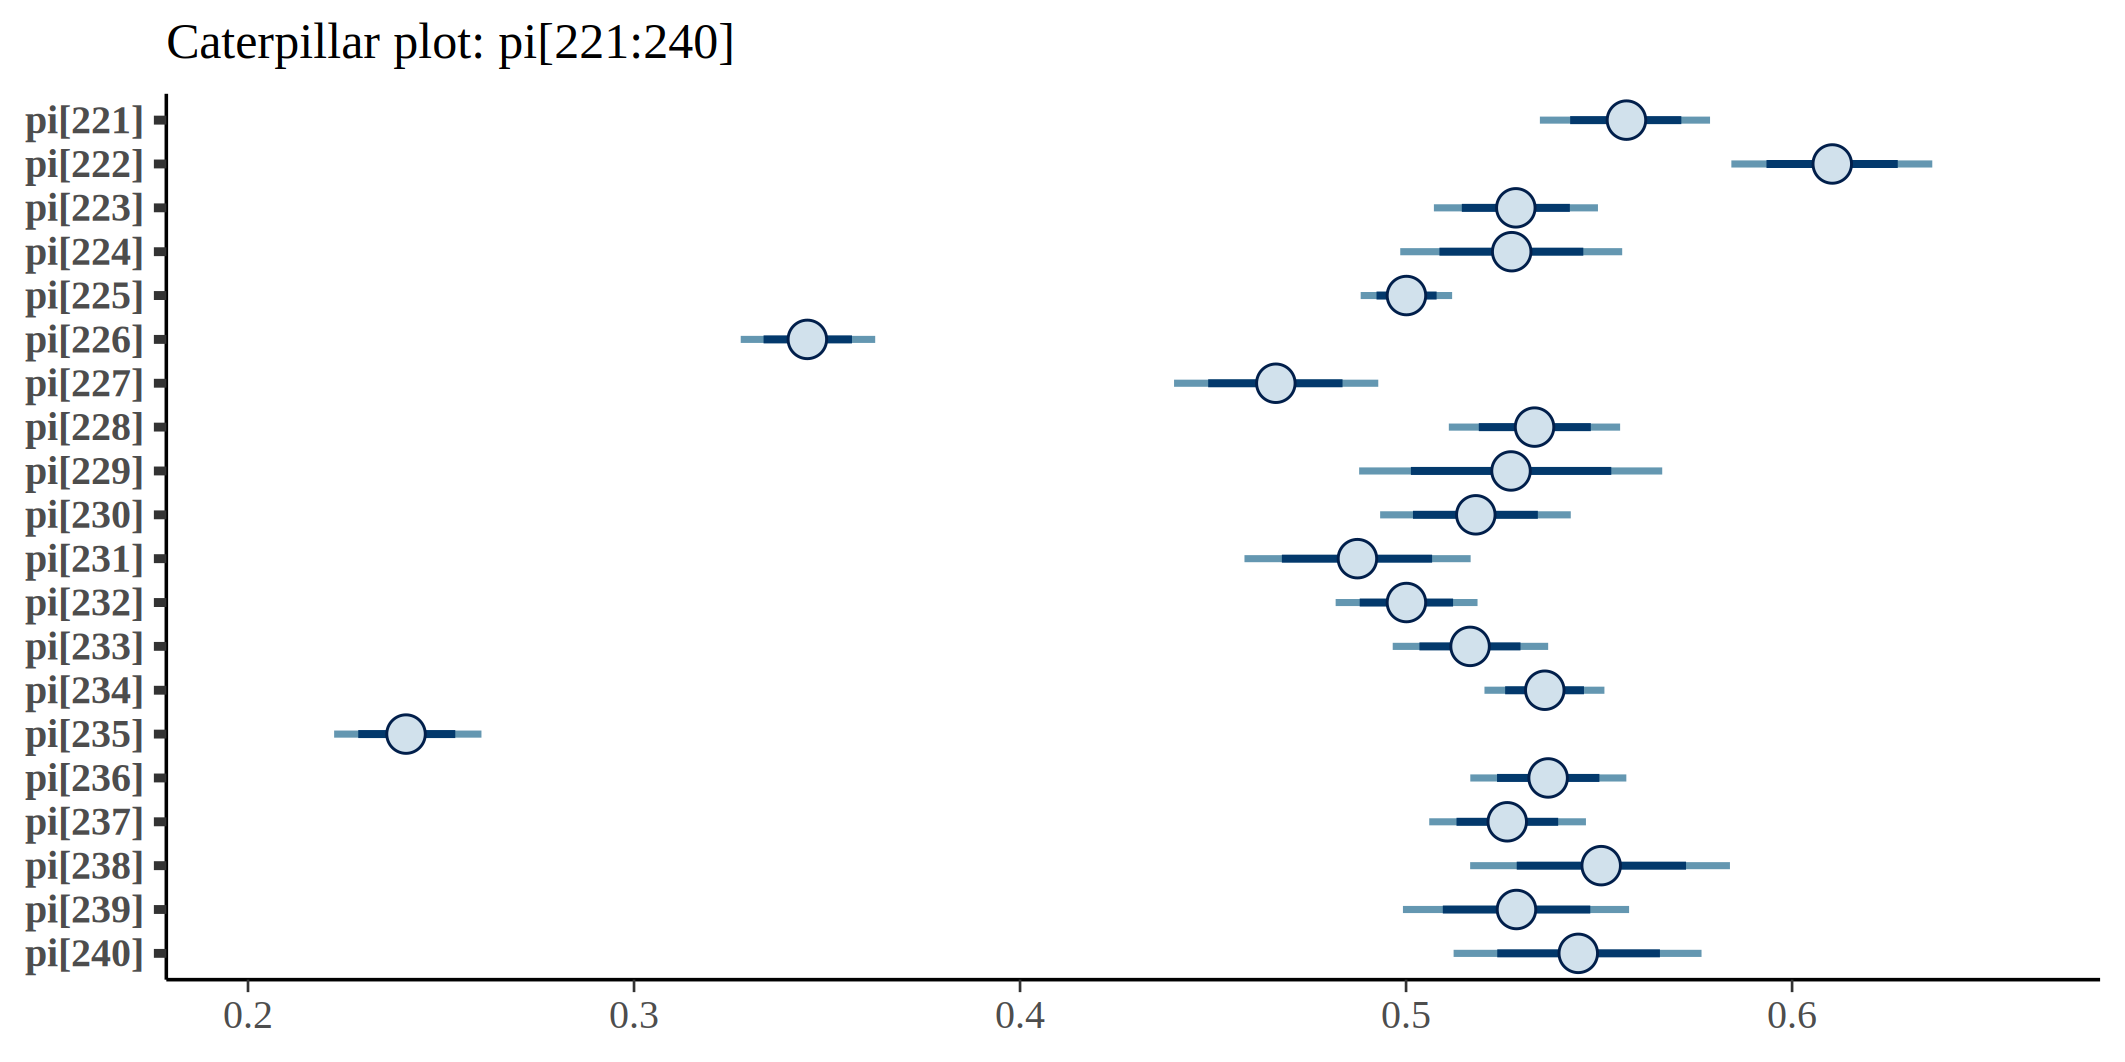
\includegraphics[width=\linewidth]{pictures/cater221-240.png}
%         \caption{pi[221:240]}
%         \label{fig:sub2_2}
%     \end{subfigure}

    
%     \begin{subfigure}{0.45\textwidth}
%         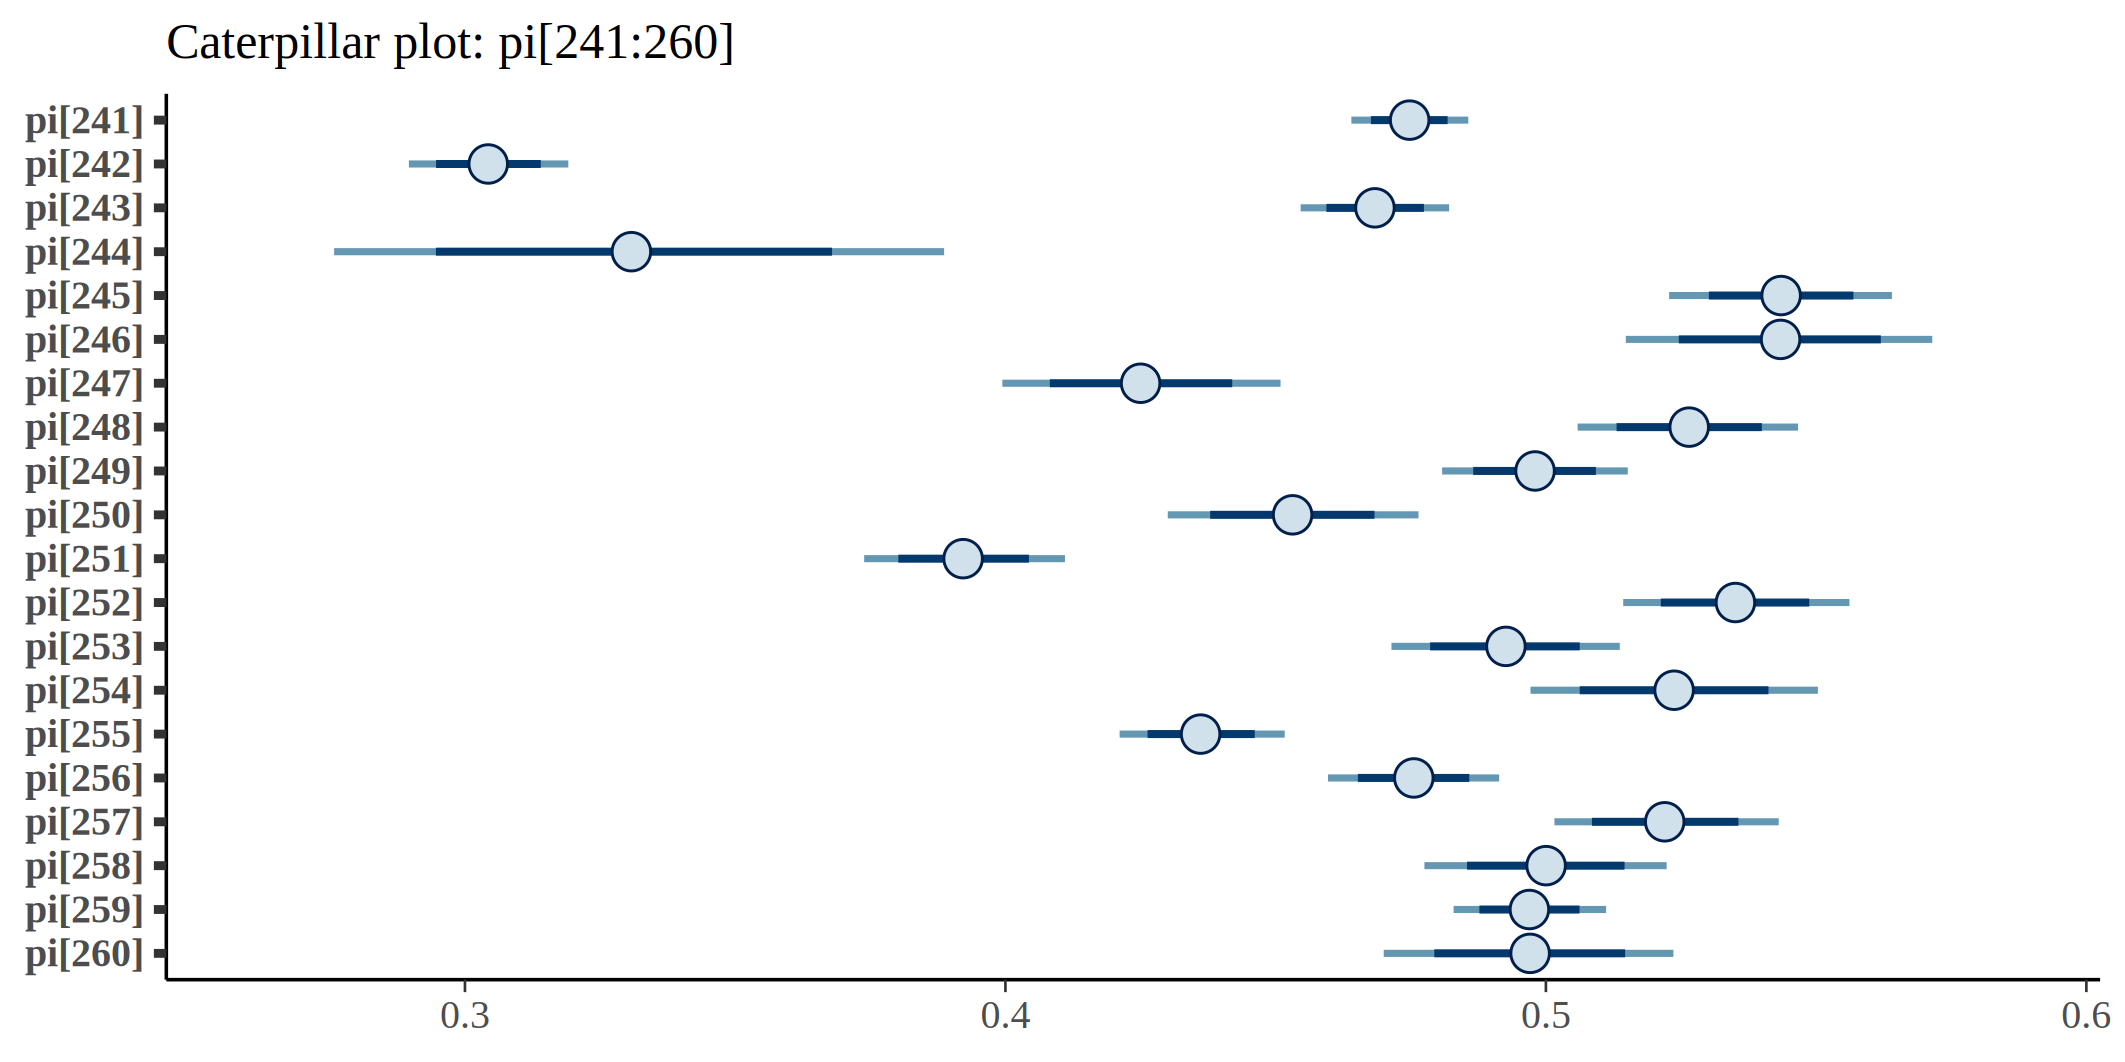
\includegraphics[width=\linewidth]{pictures/cater241-260.png}
%         \caption{pi[241:260]}
%         \label{fig:sub2_1}
%     \end{subfigure}
%     %\hfill
%     \begin{subfigure}{0.45\textwidth}
%         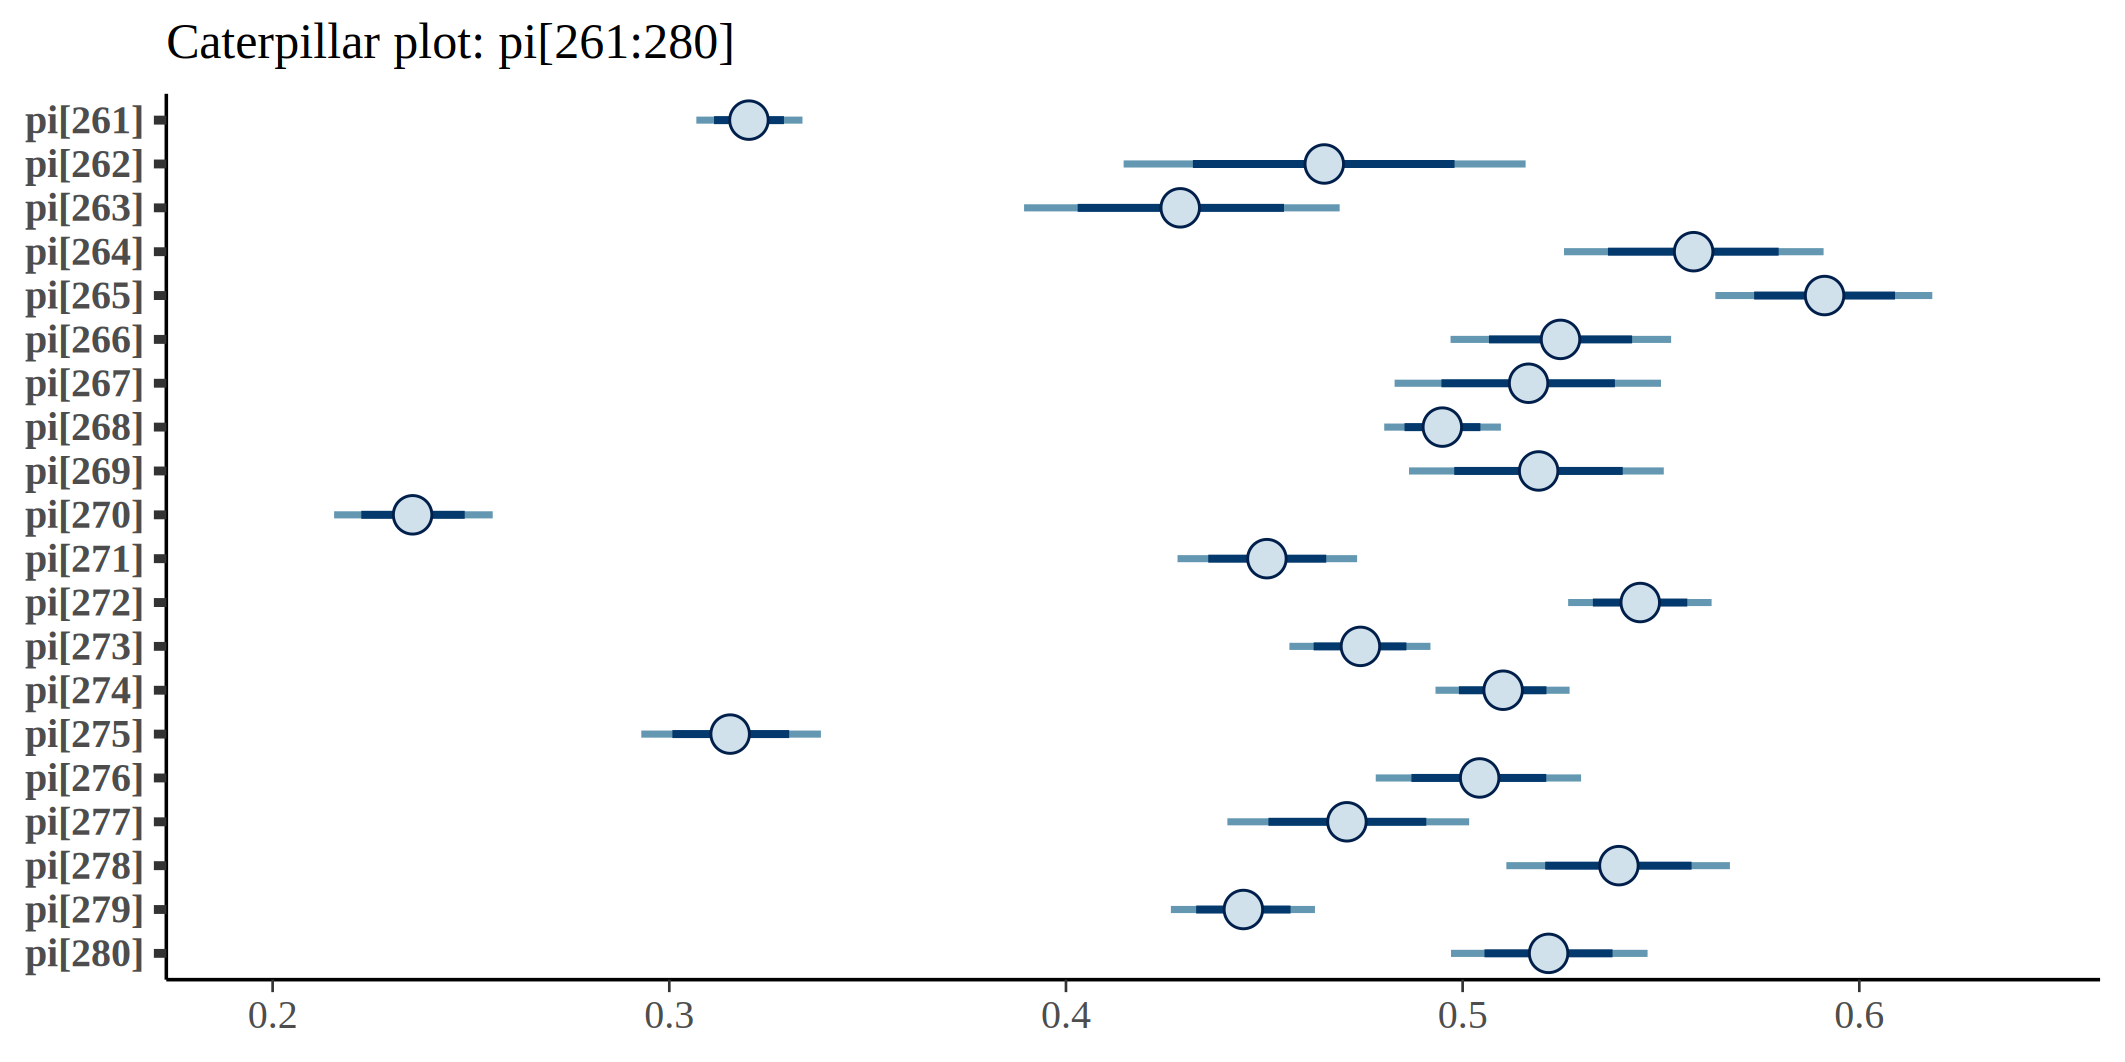
\includegraphics[width=\linewidth]{pictures/cater261-280.png}
%         \caption{pi[261:280]}
%         \label{fig:sub2_2}
%     \end{subfigure}

%     % third row
%     \vskip\baselineskip
%     \begin{subfigure}{0.45\textwidth}
%         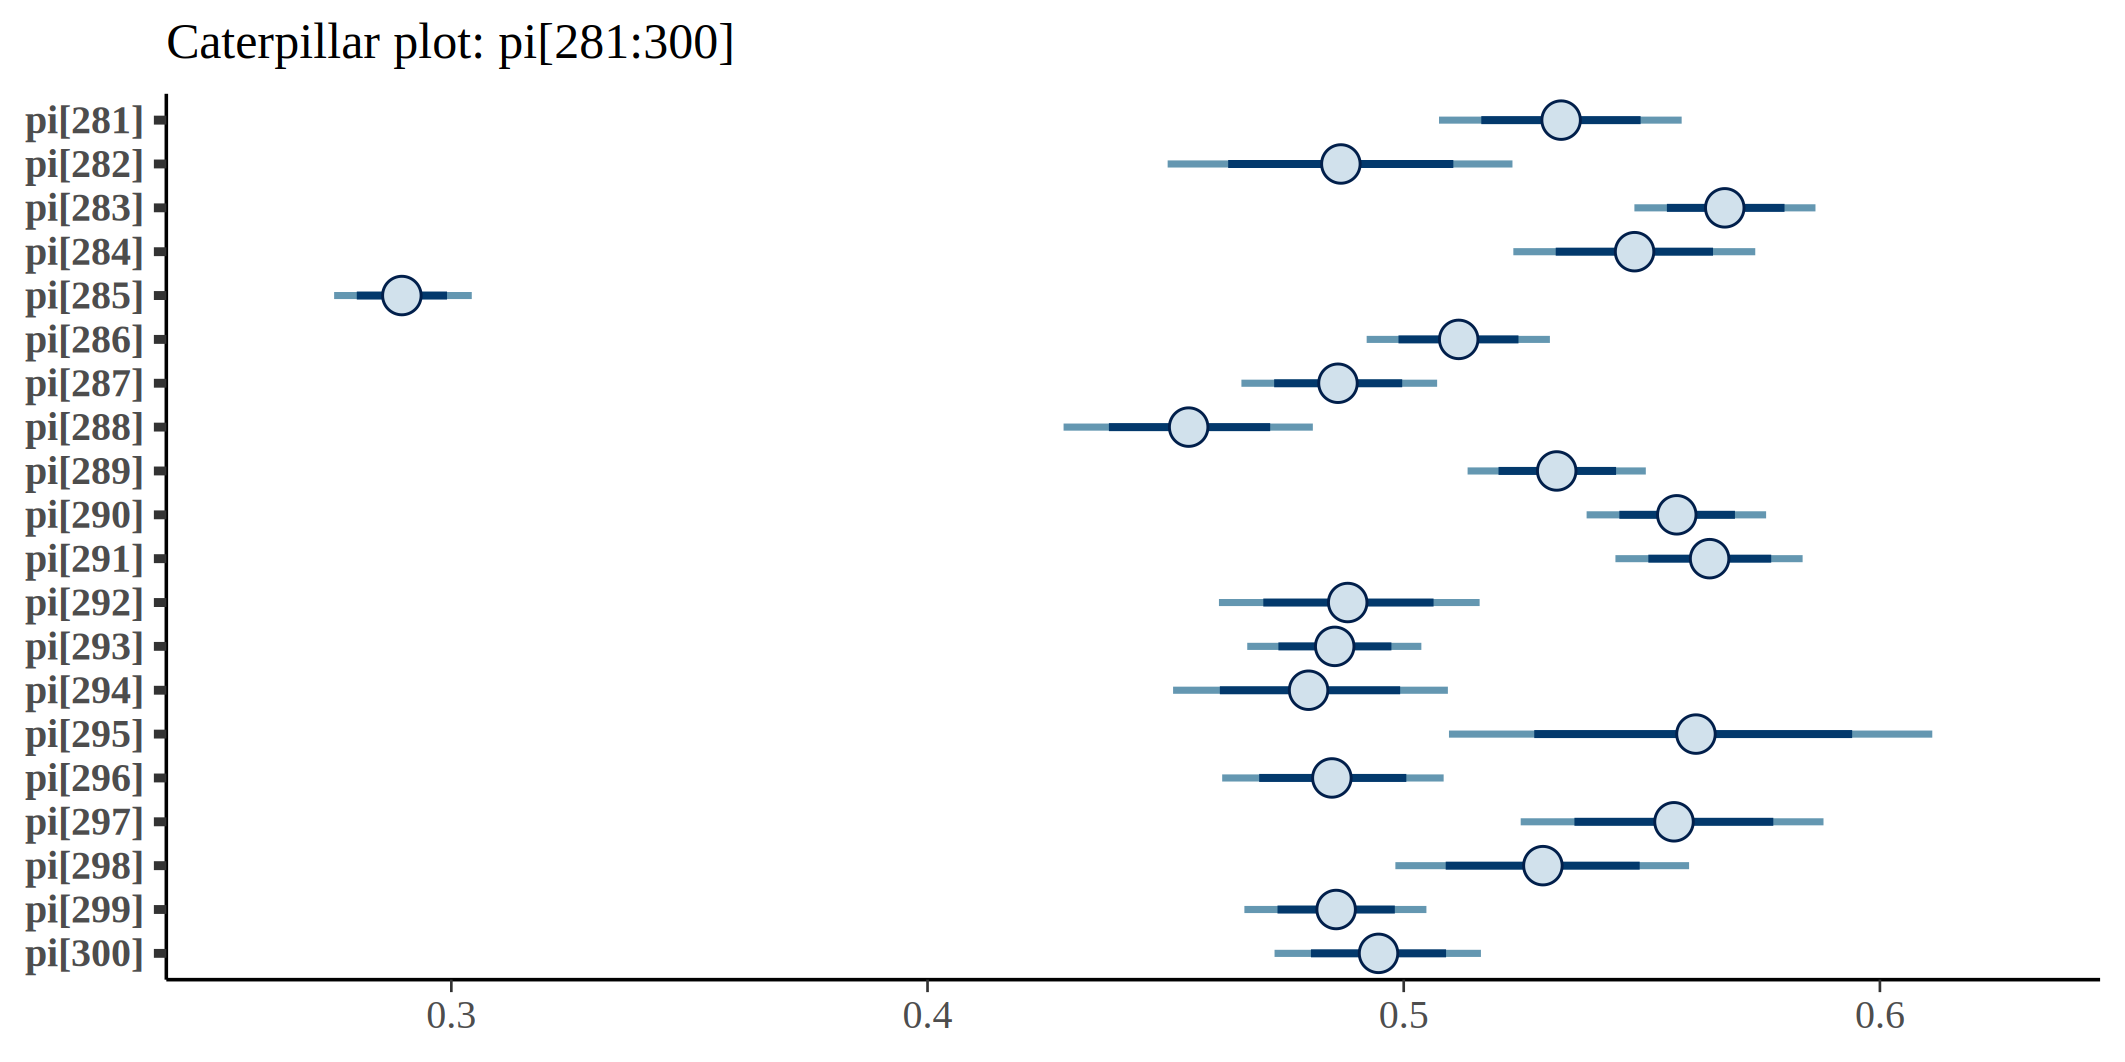
\includegraphics[width=\linewidth]{pictures/cater281-300.png}
%         \caption{pi[281:300]}
%         \label{fig:sub2_2}
%     \end{subfigure}
    
%     \caption{Posterior participation rates pi[121:300].}
%     \label{fig:caterpillar121-260}
% \end{figure}

%\FloatBarrier % Ensures the figure doesn't float past this point


\subsubsection{For which regions is $P$($\pi_i$ $<$ 0.30$|$Y ) $>$ 0.9?}

The probability $P$($\pi_i$ $<$ 0.30$|$Y ) is the posterior probability that the true participation rate $\pi_i$ for the $i$th region is less than 0.30 given the observed data $Y$. A high value of this probability as requested indicates strong evidence based on prior beliefs and data that the true parameter $\pi_i$ lies below 0.30. A number of regions meet this criteria and their posterior probabilities are indicated in brackets. These are Drogenbos ($P$=1.0000), Kraainem ($P$=1.0000), Linkebeek ($P$=0.9957), Sint-Genesius-Rode ($P$=1.000), Wemmel ($P$=1.000) and Zaventem ($P$=0.9260). For the regions Drogenbos, Kraainem, Sint-Genesius-Rode and Wemmel, there is absolute certainty that $\pi_i <$0.30.

\newpage

\subsection{Model 2}

\subsubsection{Assumed model and specification}

The number of participants in the screening program is modelled hierarichically as:

\[
    Y_{iag} \sim Binom(\pi_{iag}, N_{iag}),
\]

while assuming that the participation rates are impacted by age and gender but are clustered within municipalities. As a logistic random effects model, this is: 

\[
    logit(\pi_{iag}) = \alpha + \beta a + \gamma g + b_i \qquad b_i \sim N(0, \sigma^2)
\]

\noindent where $\beta a$ is the effect of age modelled as dummies for the different age groups, $\gamma g$ is the gender effect and $\alpha$ is the intercept. 

All parameters are given vague priors. The $\alpha$, $\beta$ and $\gamma$ parameters are given a normal prior. The $b_i$ parameter is given a normal prior with normal and uniform hyperpriors for the hyperparameters mean ($\mu$) and standard deviation ($\sigma$) respectively for the random effects. The initial values of $\alpha$, $\beta$, $\gamma$ and $\mu$ were randomly generated from a normal distribution. All these parameters, including $\pi_{iag}$ are monitored. Three Markov chains each with 10,000 iterations and a burn-in of 5,000 iterations were used. The thinning rate was left to the default value of 5. 


\subsubsection{ Compare convergence for the hierarchically centered versus uncentered model.}

%The MCerror was generally higher in the hierarchically centered model as compared to the uncentered model for the $\pi$ parameters. 

Graphical tests and formal diagnostics are used to assess convergence for the uncentered model.  Due to the many $\pi_{iag}$ parameters, relevant plots are not shown for brevity. The results of the diagnostics for the other parameters are as follows:

\textbf{Trace plot}: The posterior distribution is rapidly explored by all chains for $\beta$, $\gamma$, $\sigma$, $\mu$ and $\pi_{iag}$. There are no gross deviations from stationarity. As a sample, the traceplots for $\beta$, $\gamma$, $\sigma$ and $\alpha$ are shown in figure \ref{fig:traceplotsm2}.

\begin{figure}[h!]
    \centering
    % First row
    \begin{subfigure}{0.45\textwidth}
        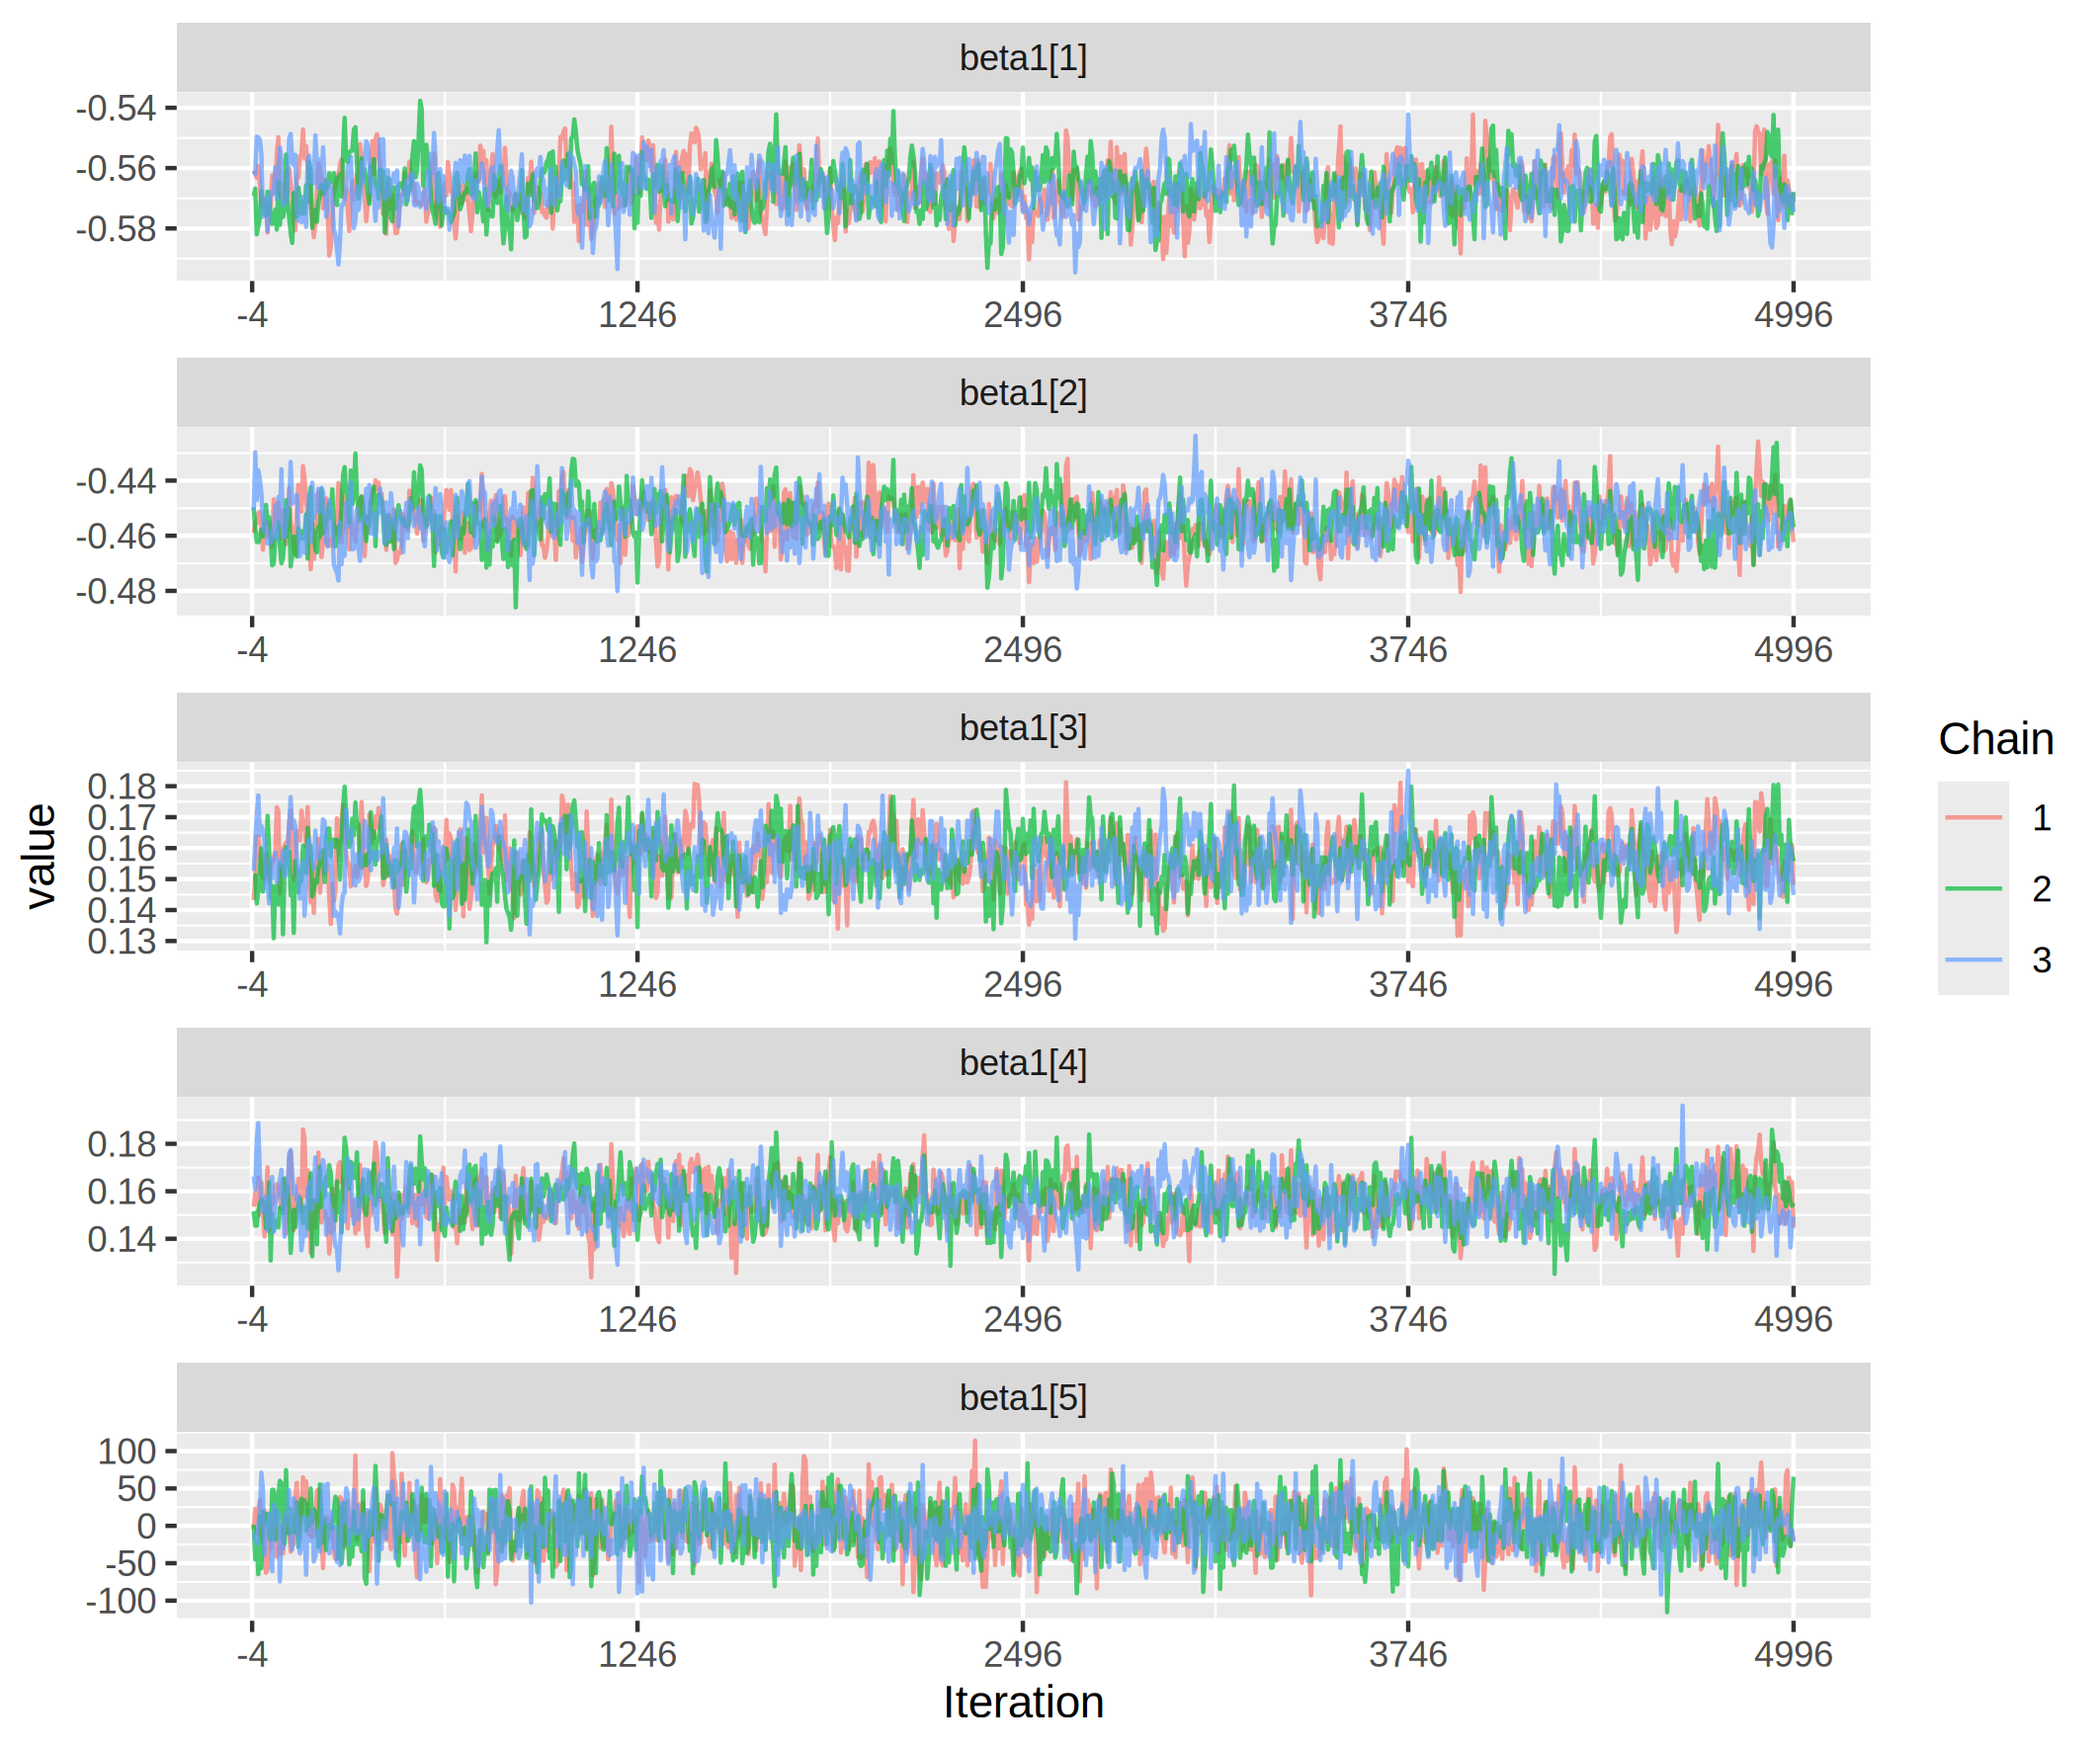
\includegraphics[width=\linewidth]{pictures/mod2/mod2trace_beta.png}
        %\caption{pi[1:20]}
        %\label{fig:sub1_1}
    \end{subfigure}
    %\hfill
    \begin{subfigure}{0.45\textwidth}
        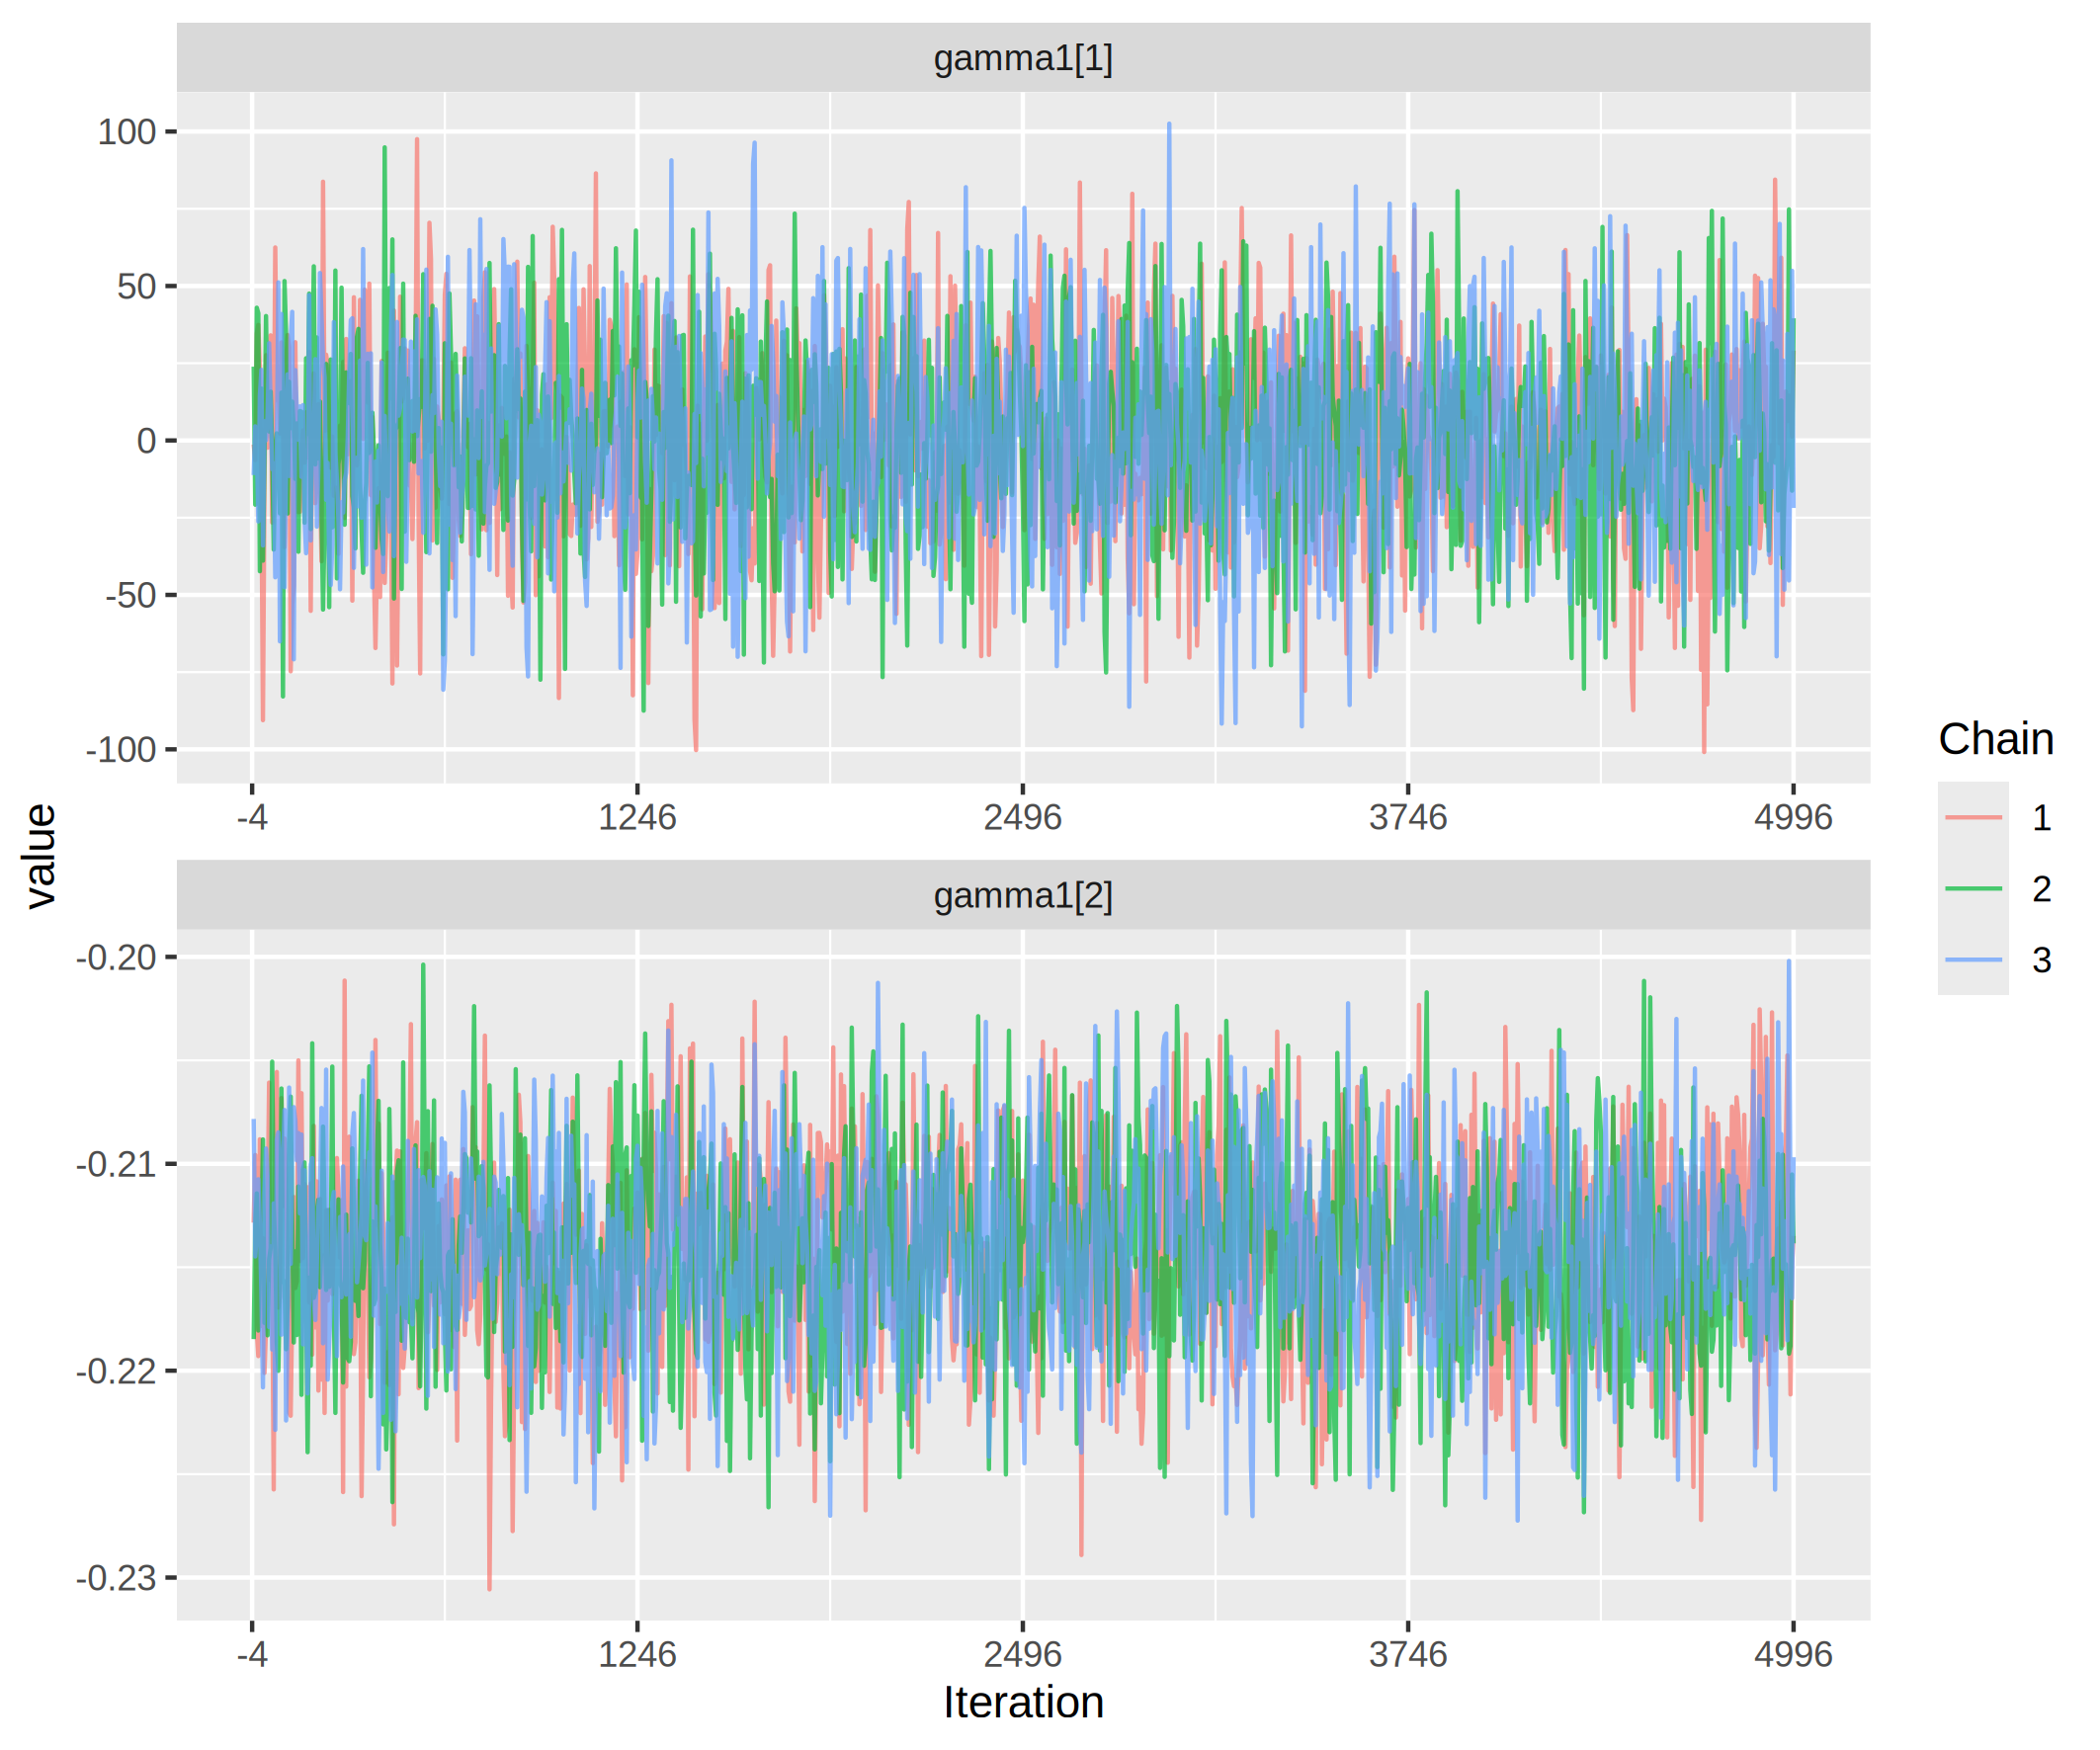
\includegraphics[width=\linewidth]{pictures/mod2/mod2trace_gamma.png}
        %\caption{pi[21:40]}
        %\label{fig:sub1_2}
    \end{subfigure}

    % Second row
    \vskip\baselineskip
    \begin{subfigure}{0.45\textwidth}
        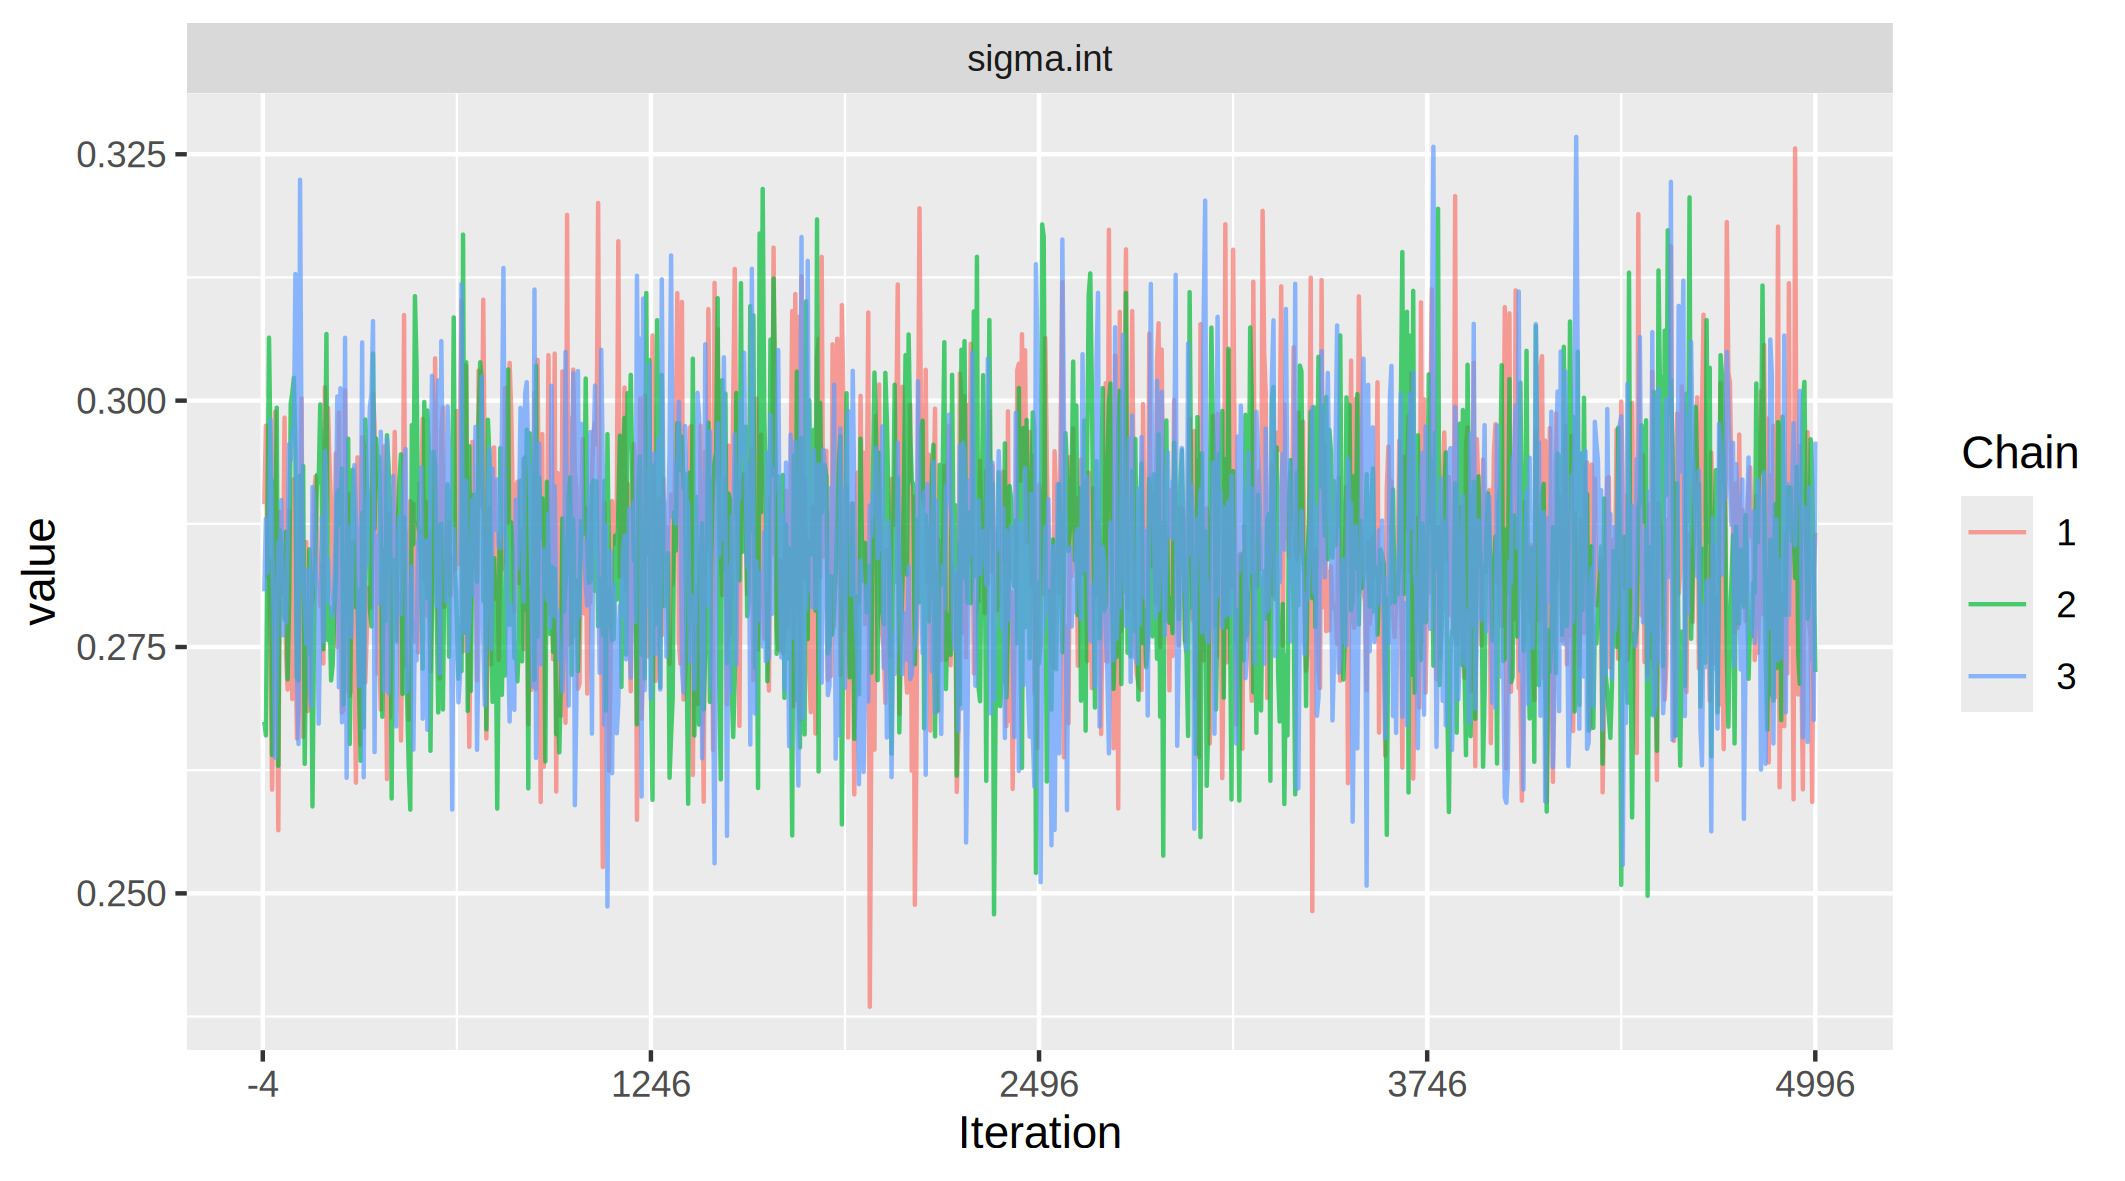
\includegraphics[width=\linewidth]{pictures/mod2/mod2trace_sigmaint.png}
        %\caption{pi[41:60]}
        %\label{fig:sub2_1}
    \end{subfigure}
    %\hfill
    \begin{subfigure}{0.45\textwidth}
        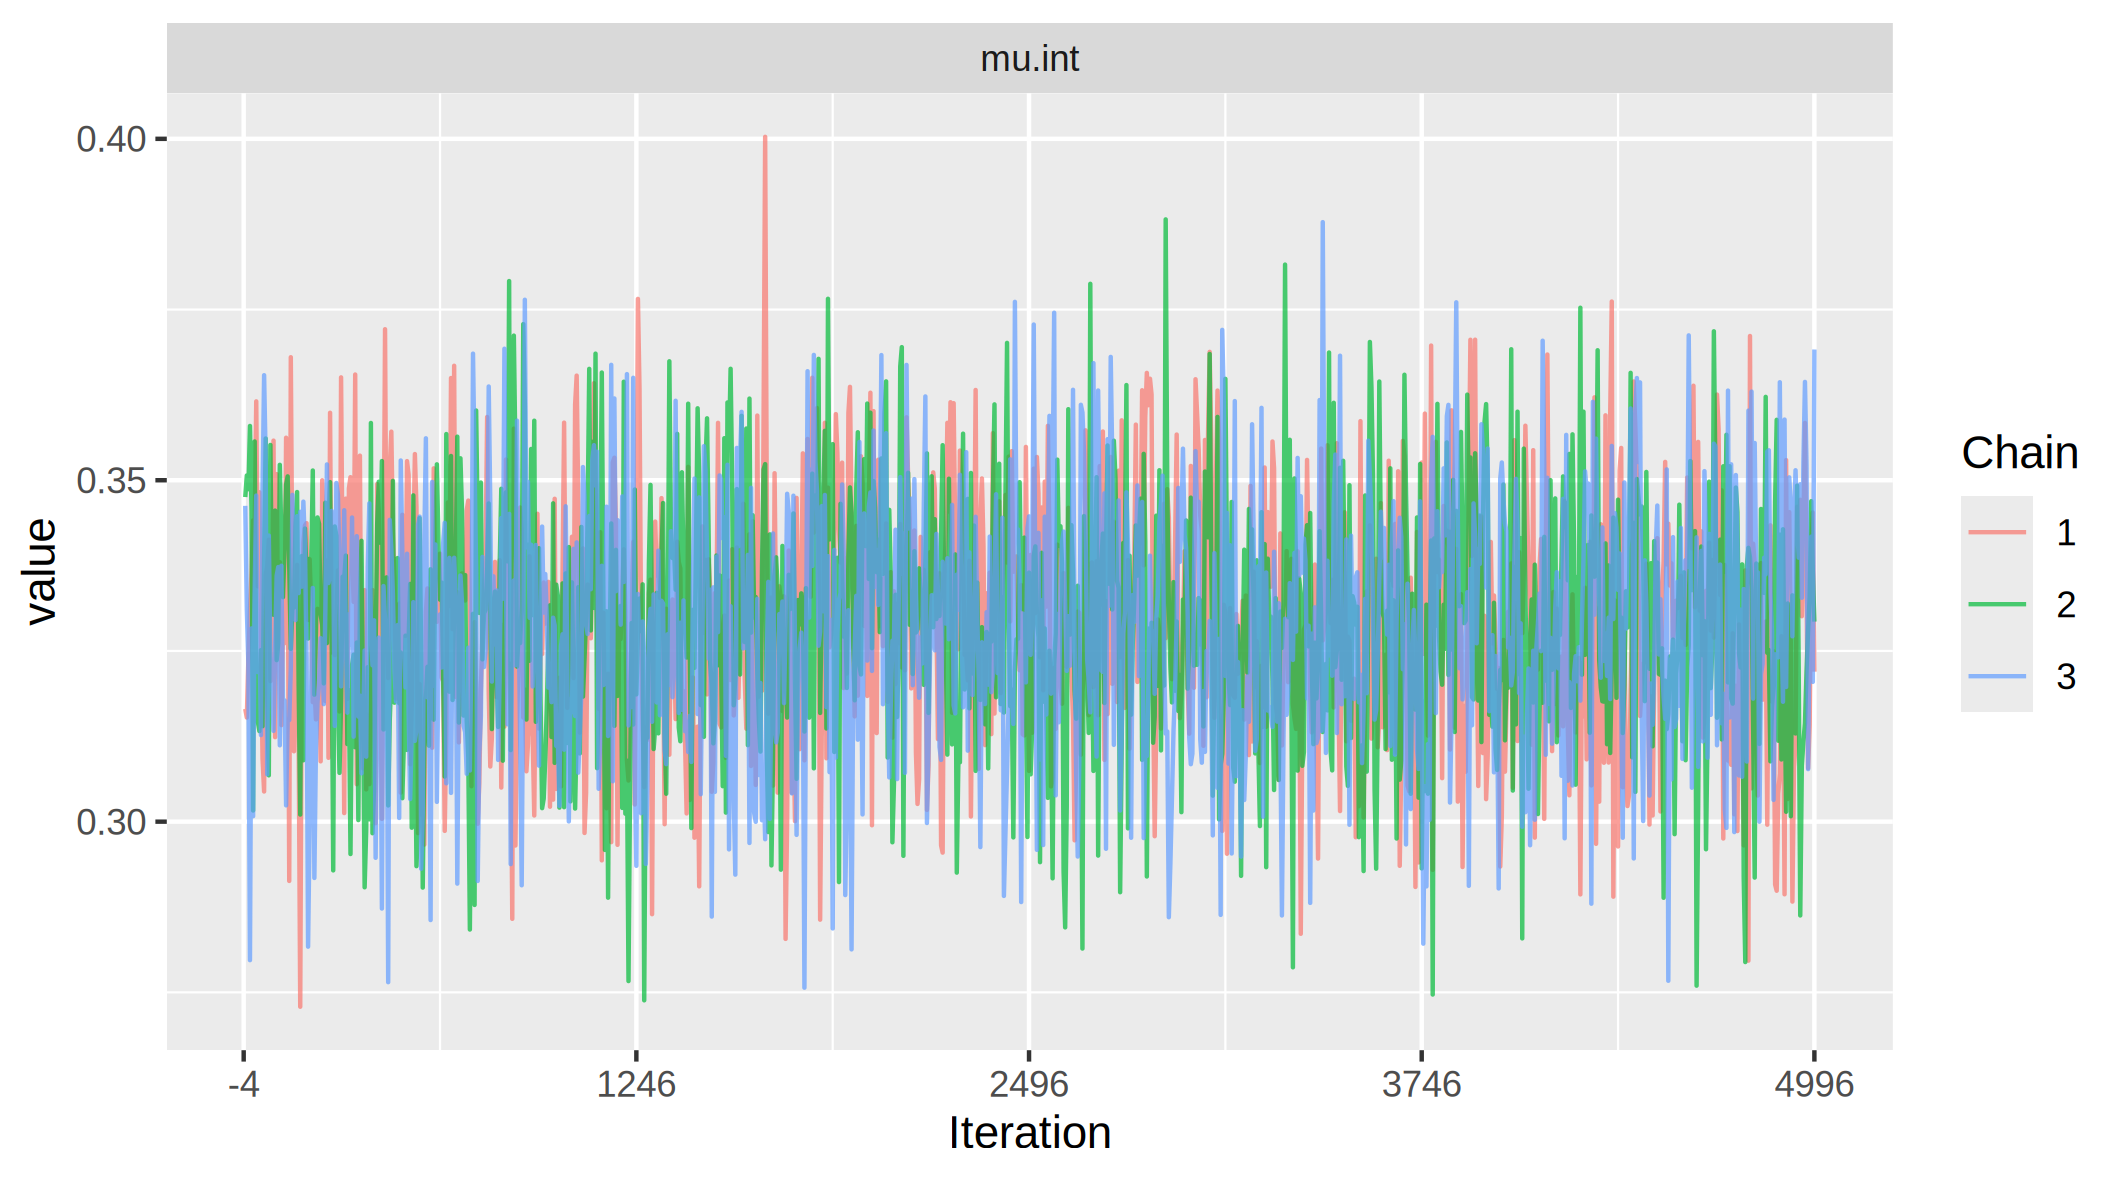
\includegraphics[width=\linewidth]{pictures/mod2/mod2trace_muint.png}
        %\caption{pi[61:80]}
        %\label{fig:sub2_2}
    \end{subfigure}
    
    \caption{traceplots for $\beta$, $\gamma$, $\sigma$ and $\alpha$ }
    \label{fig:traceplotsm2}
\end{figure}

\textbf{Autocorrelation plot}: The autocorrelation plots for some parameters ($\beta$, $\gamma$, $\sigma$ and $\alpha$) are shown in figure \ref{fig:autocorrM2}. There is good mixing rates for all parameters including $\pi_{iag}$ (not shown).

\begin{figure}[h!]
    \centering
    % First row
    \begin{subfigure}{0.45\textwidth}
        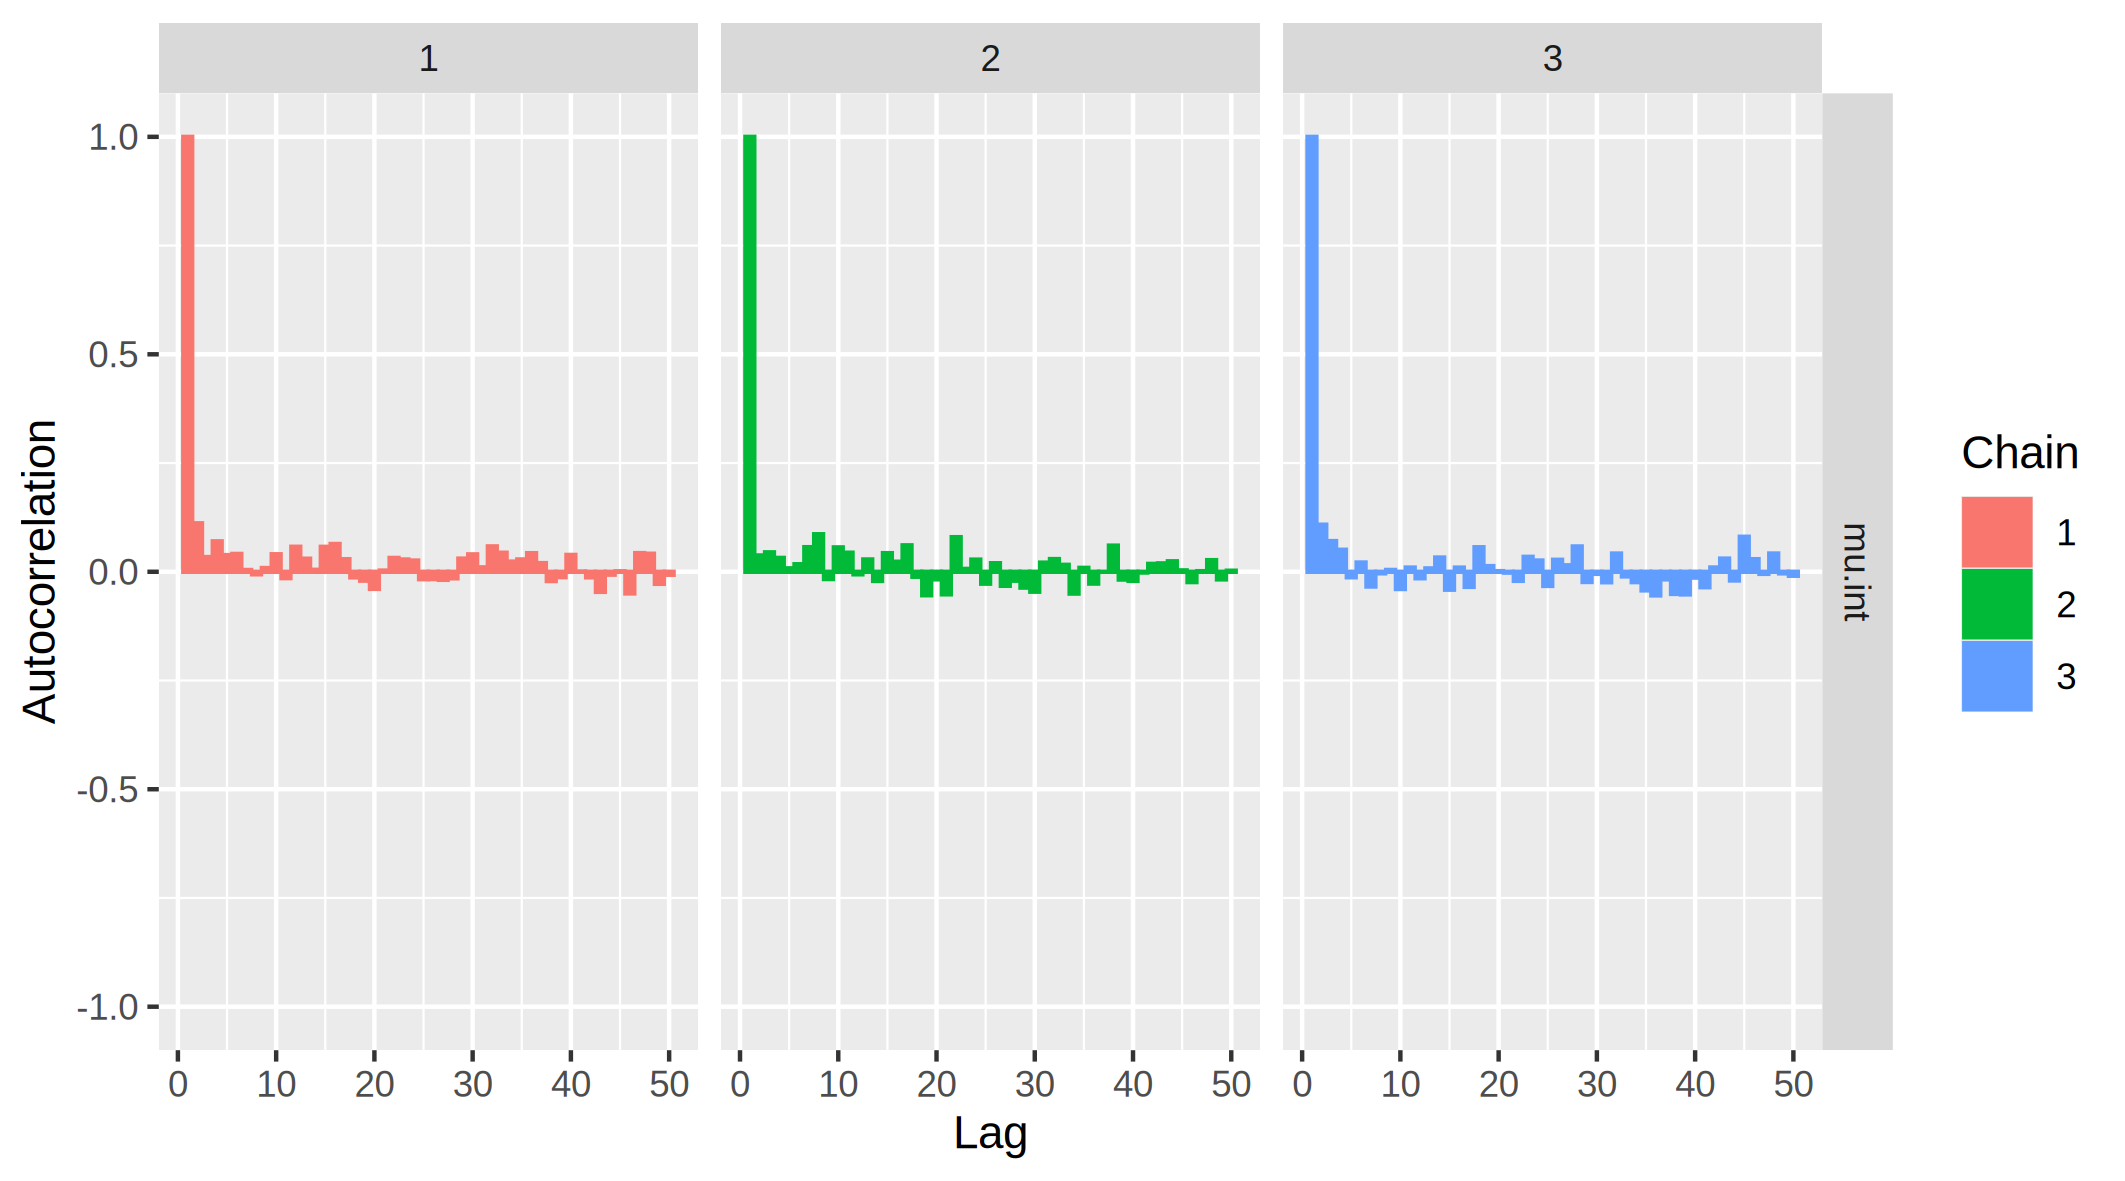
\includegraphics[width=\linewidth]{pictures/mod2/mod2autocorr_muint.png}
        %\caption{pi[1:20]}
        %\label{fig:sub1_1}
    \end{subfigure}
    %\hfill
    \begin{subfigure}{0.45\textwidth}
        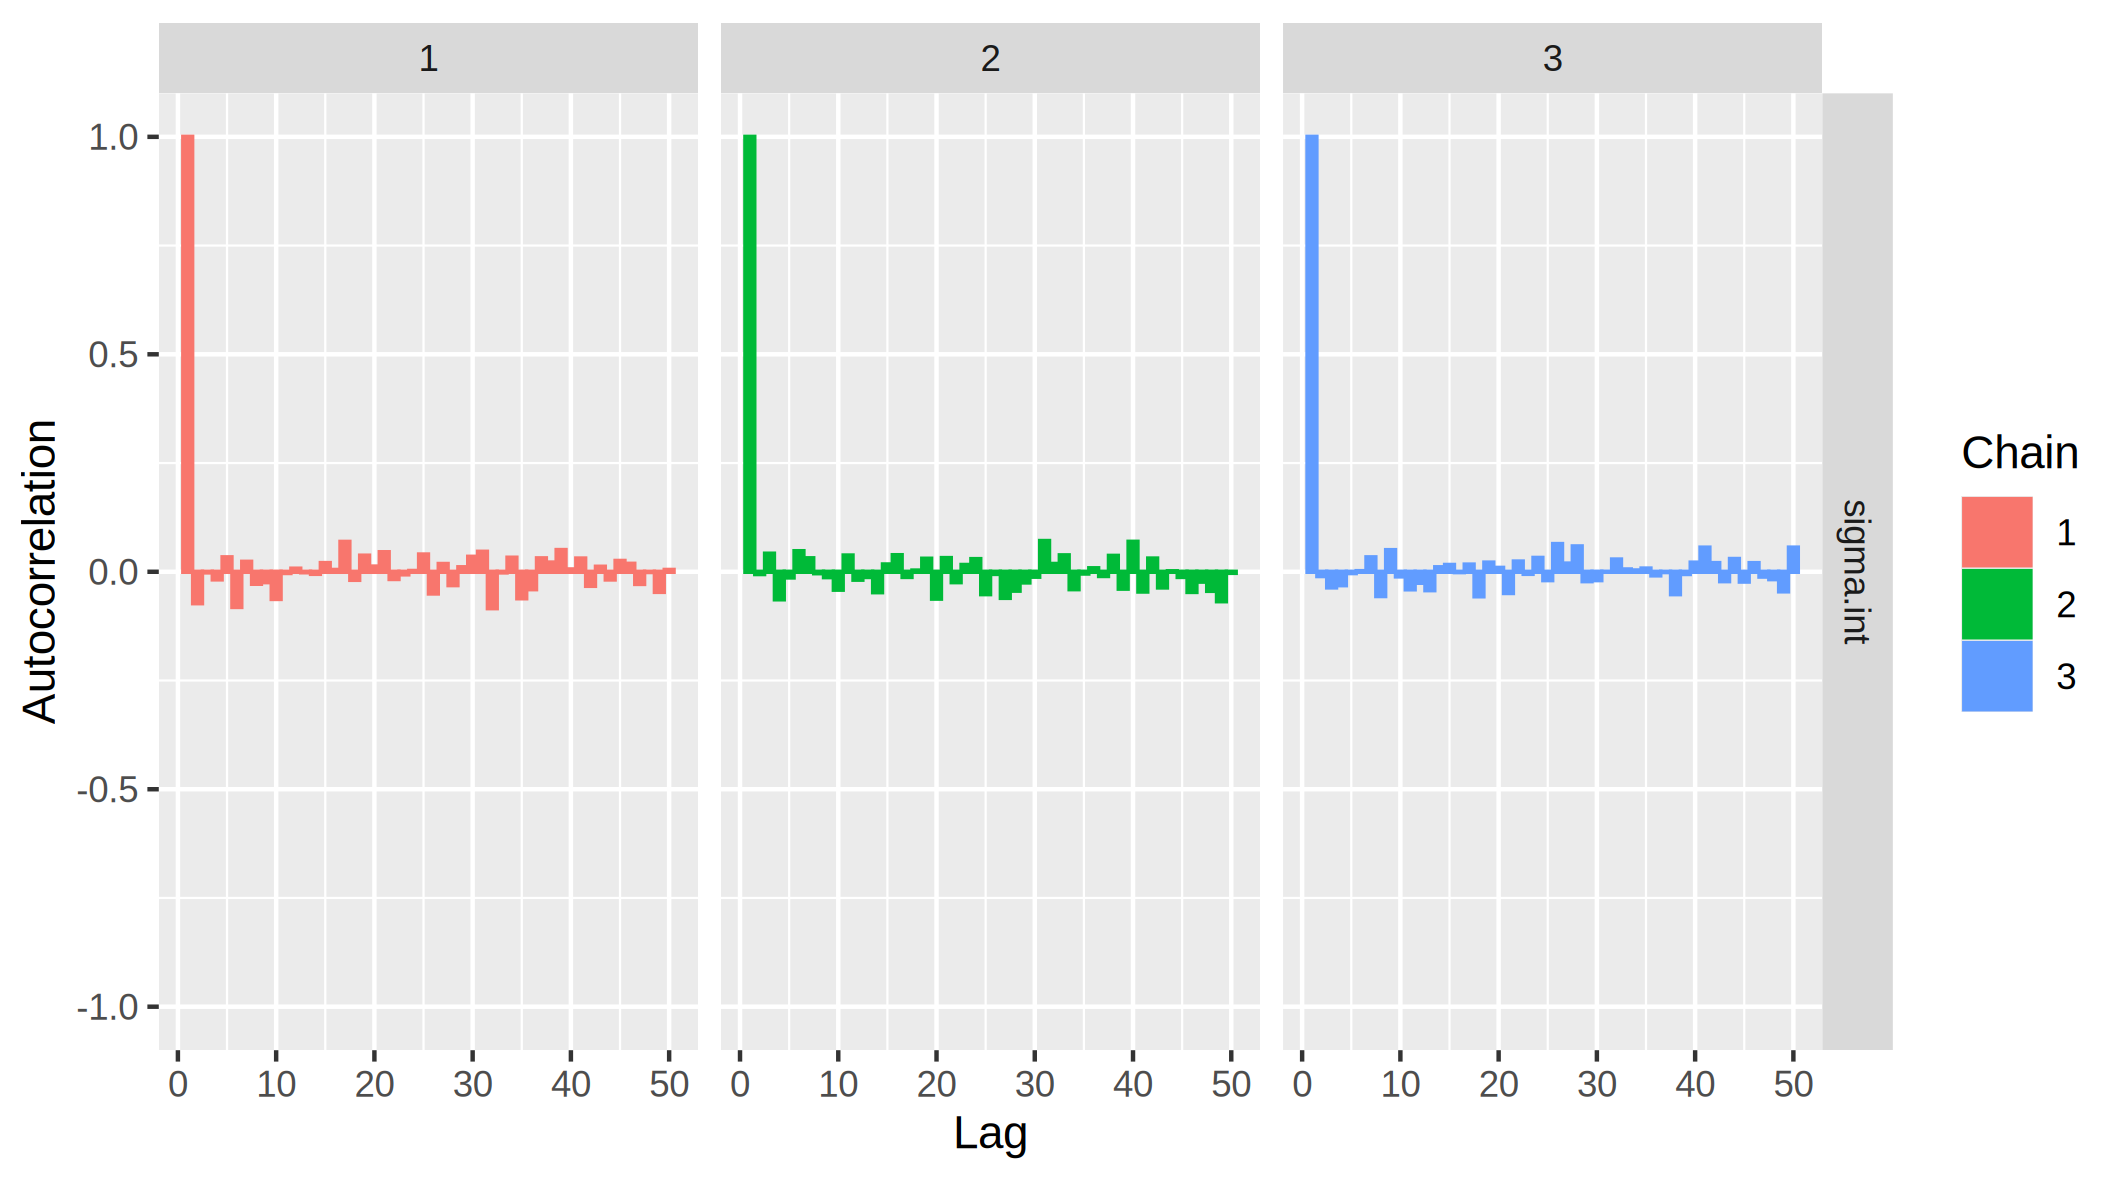
\includegraphics[width=\linewidth]{pictures/mod2/mod2autocorr_sigmaint.png}
        %\caption{pi[21:40]}
        %\label{fig:sub1_2}
    \end{subfigure}

    % Second row
    \vskip\baselineskip
    \begin{subfigure}{0.45\textwidth}
        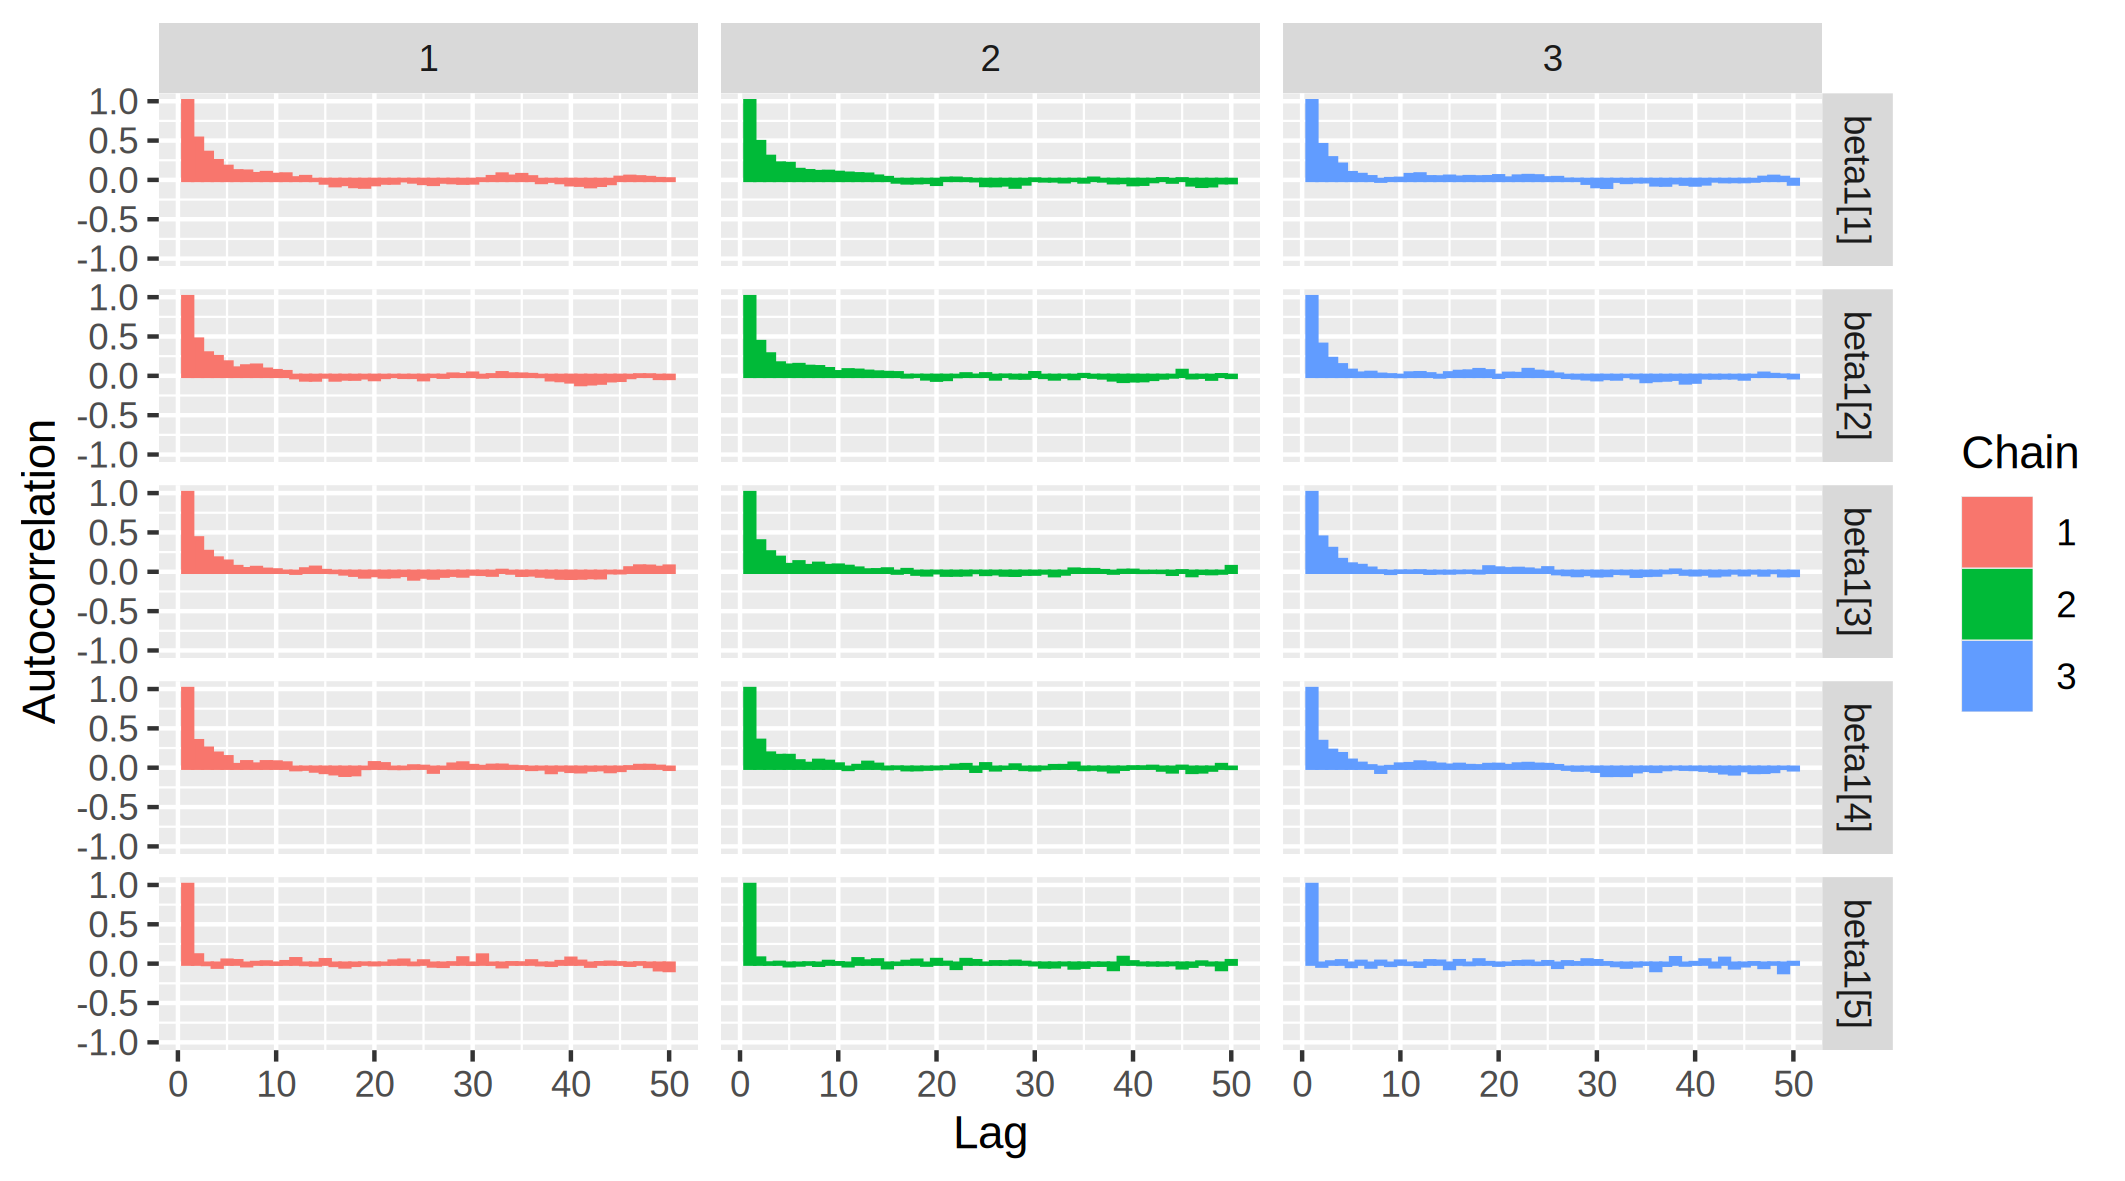
\includegraphics[width=\linewidth]{pictures/mod2/mod2autocorr_beta.png}
        %\caption{pi[41:60]}
        %\label{fig:sub2_1}
    \end{subfigure}
    %\hfill
    \begin{subfigure}{0.45\textwidth}
        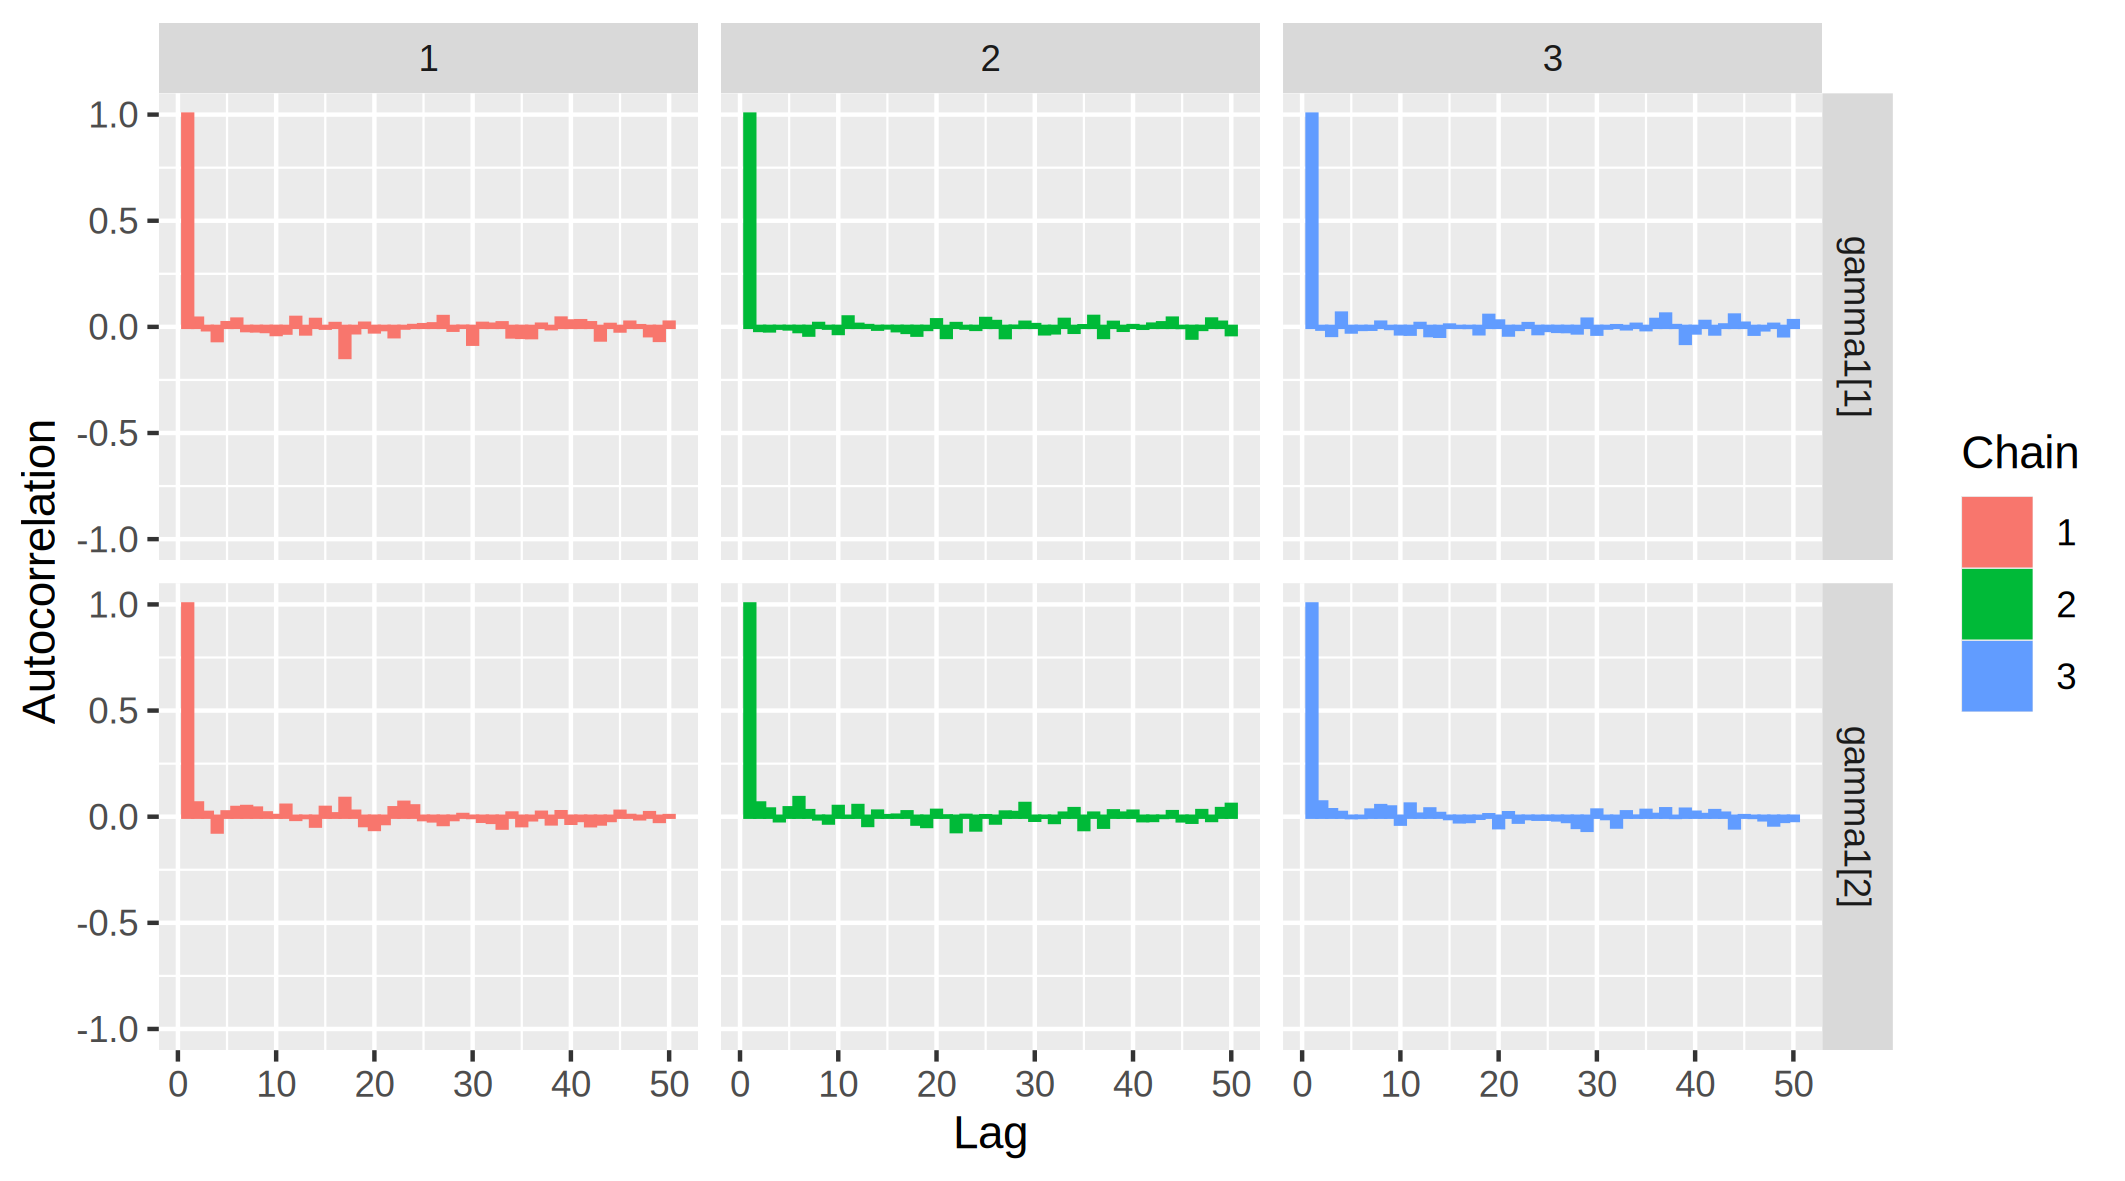
\includegraphics[width=\linewidth]{pictures/mod2/mod2autocorr_gamma.png}
        %\caption{pi[61:80]}
        %\label{fig:sub2_2}
    \end{subfigure}
    
    \caption{Autocorrelation plots for $\beta$, $\gamma$, $\sigma$ and $\alpha$}
    \label{fig:autocorrM2}
\end{figure}
\FloatBarrier % Ensures the figure doesn't float past this point

\textbf{Running-mean plots}: The running-mean plots (sample in figure \ref{fig:runningmeanM2}) show a stable behaviour for $\beta$, $\gamma$, $\sigma$, $\mu$ and $\pi_{iag}$ indicating stationarity.

\begin{figure}[h!]
    \centering
    % First row
    \begin{subfigure}{0.45\textwidth}
        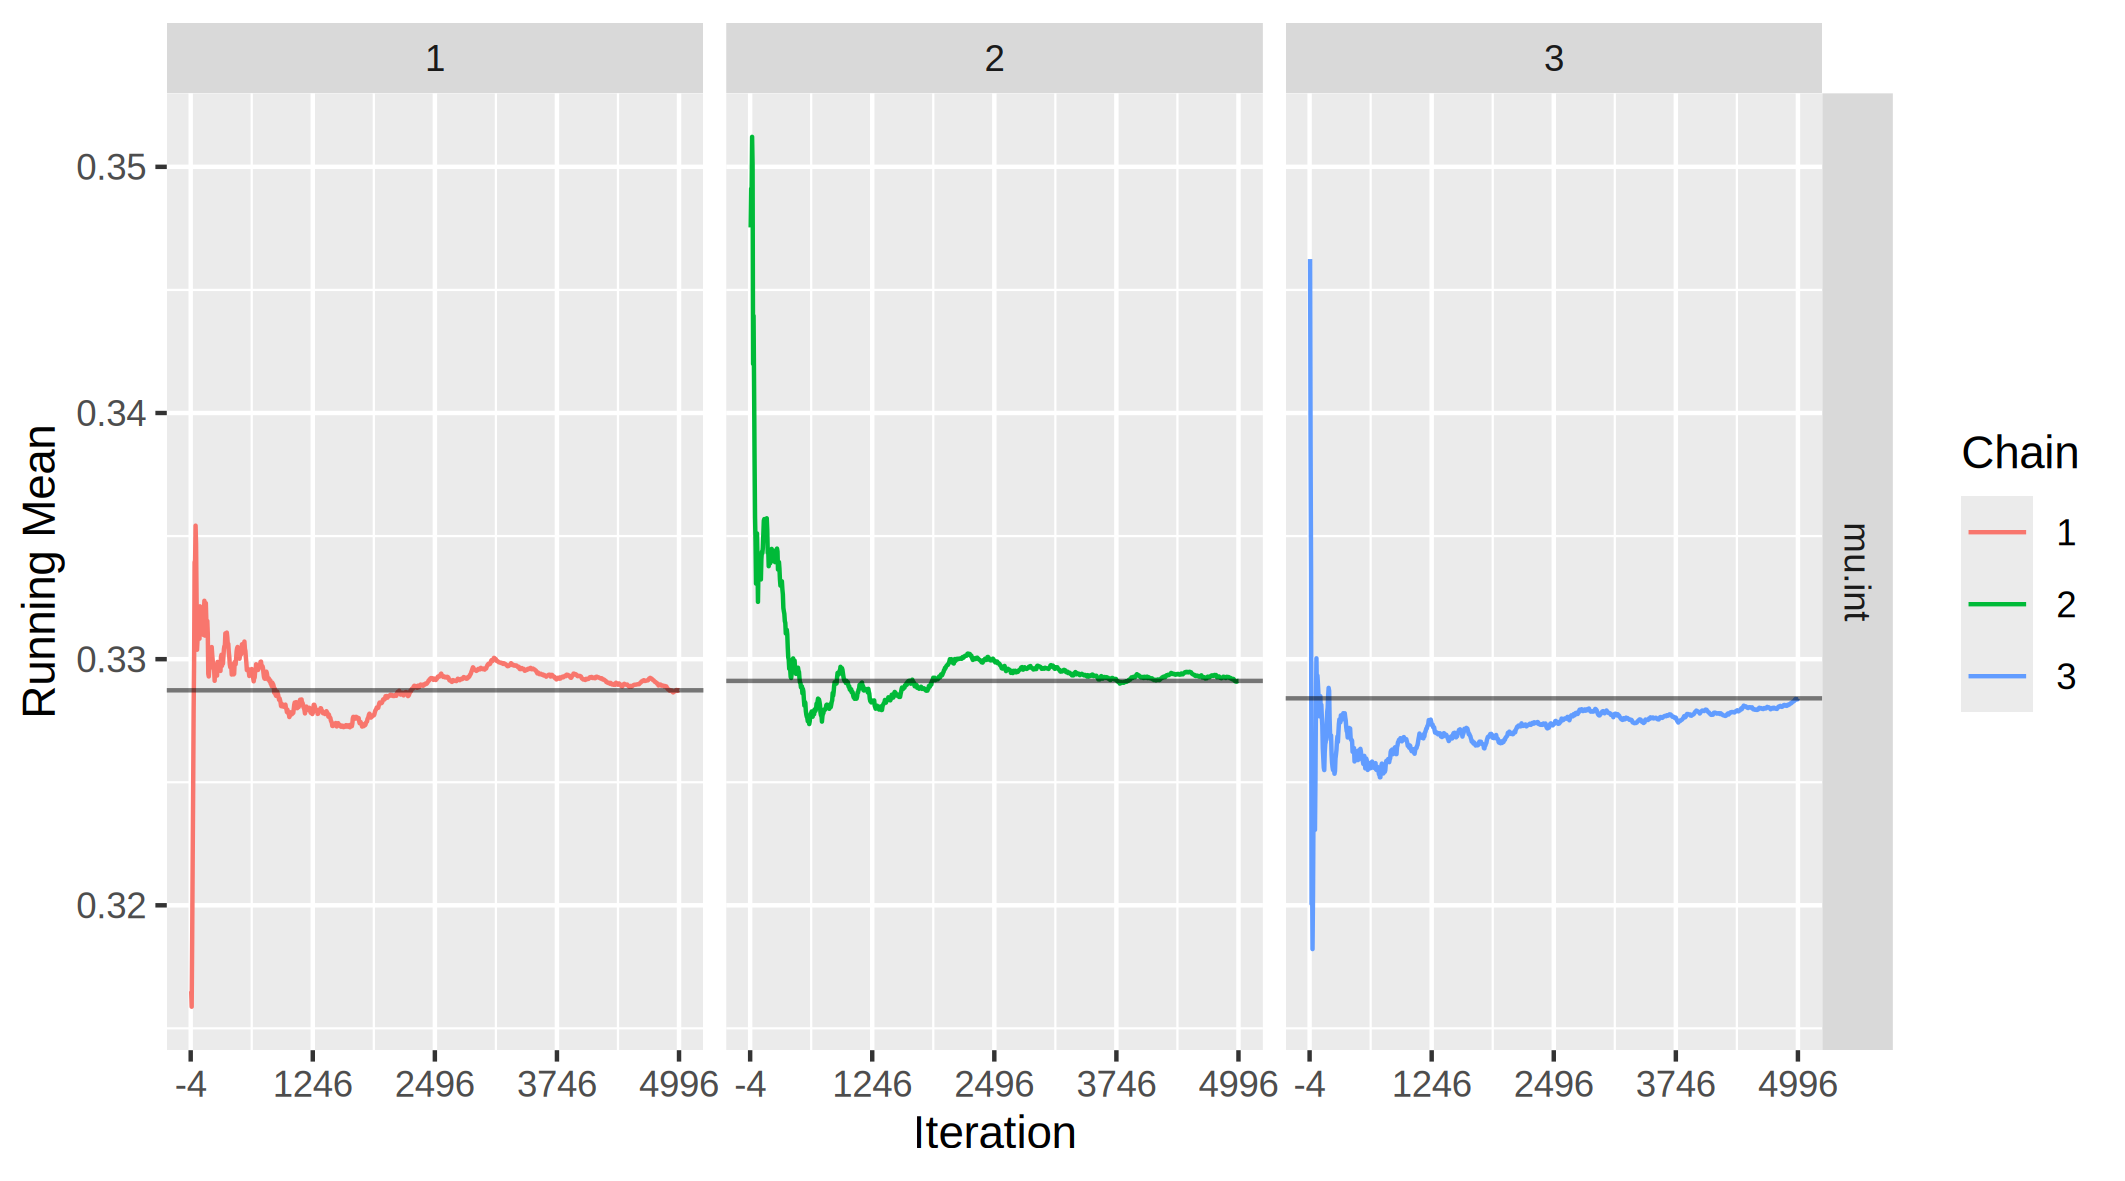
\includegraphics[width=\linewidth]{pictures/mod2/mod2rmean_muint.png}
        %\caption{pi[1:20]}
        %\label{fig:sub1_1}
    \end{subfigure}
    %\hfill
    \begin{subfigure}{0.45\textwidth}
        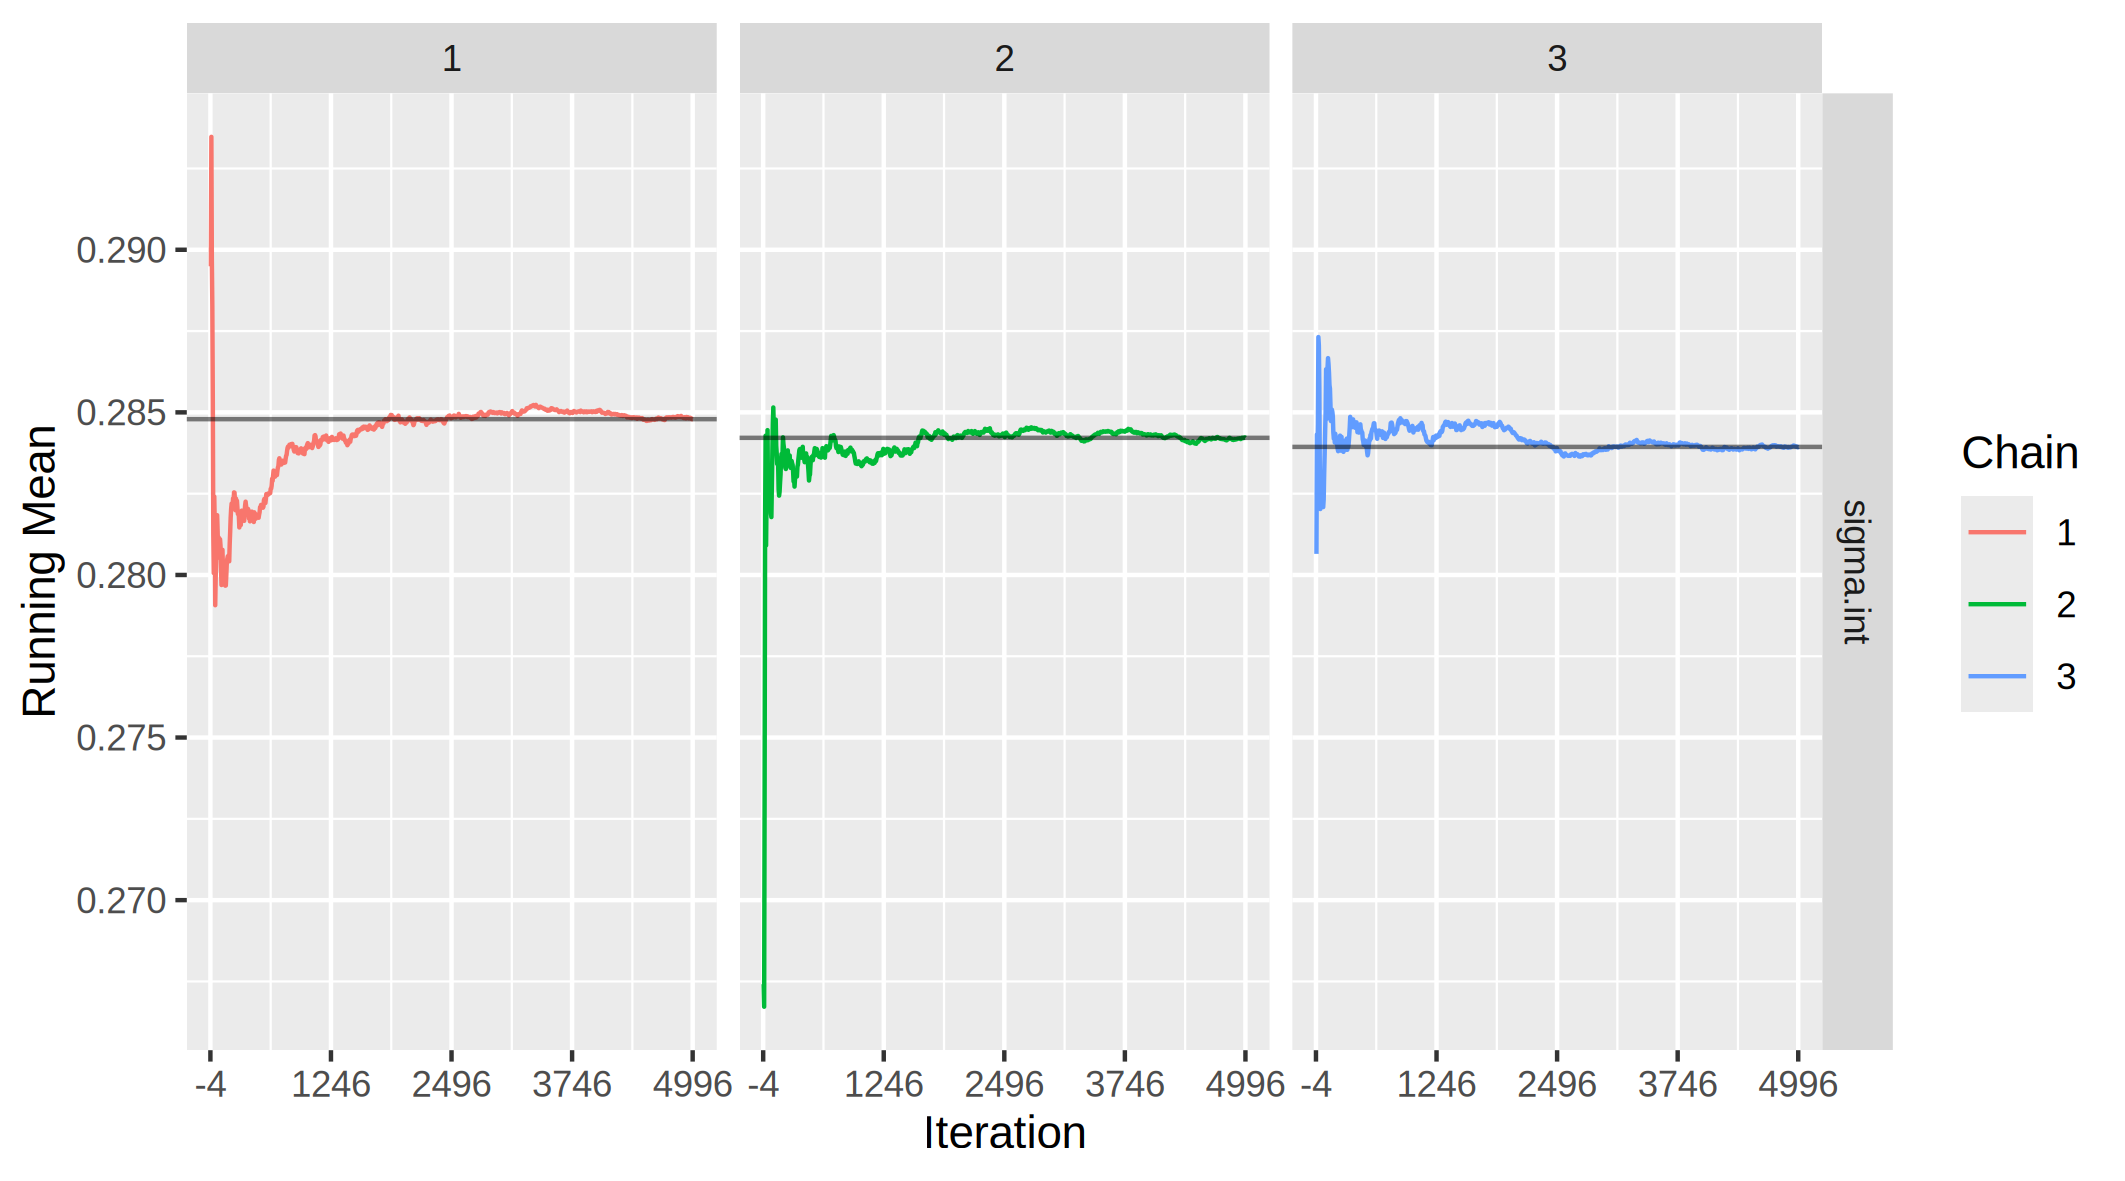
\includegraphics[width=\linewidth]{pictures/mod2/mod2rmean_sigmaint.png}
        %\caption{pi[21:40]}
        %\label{fig:sub1_2}
    \end{subfigure}

    % Second row
    \vskip\baselineskip
    \begin{subfigure}{0.45\textwidth}
        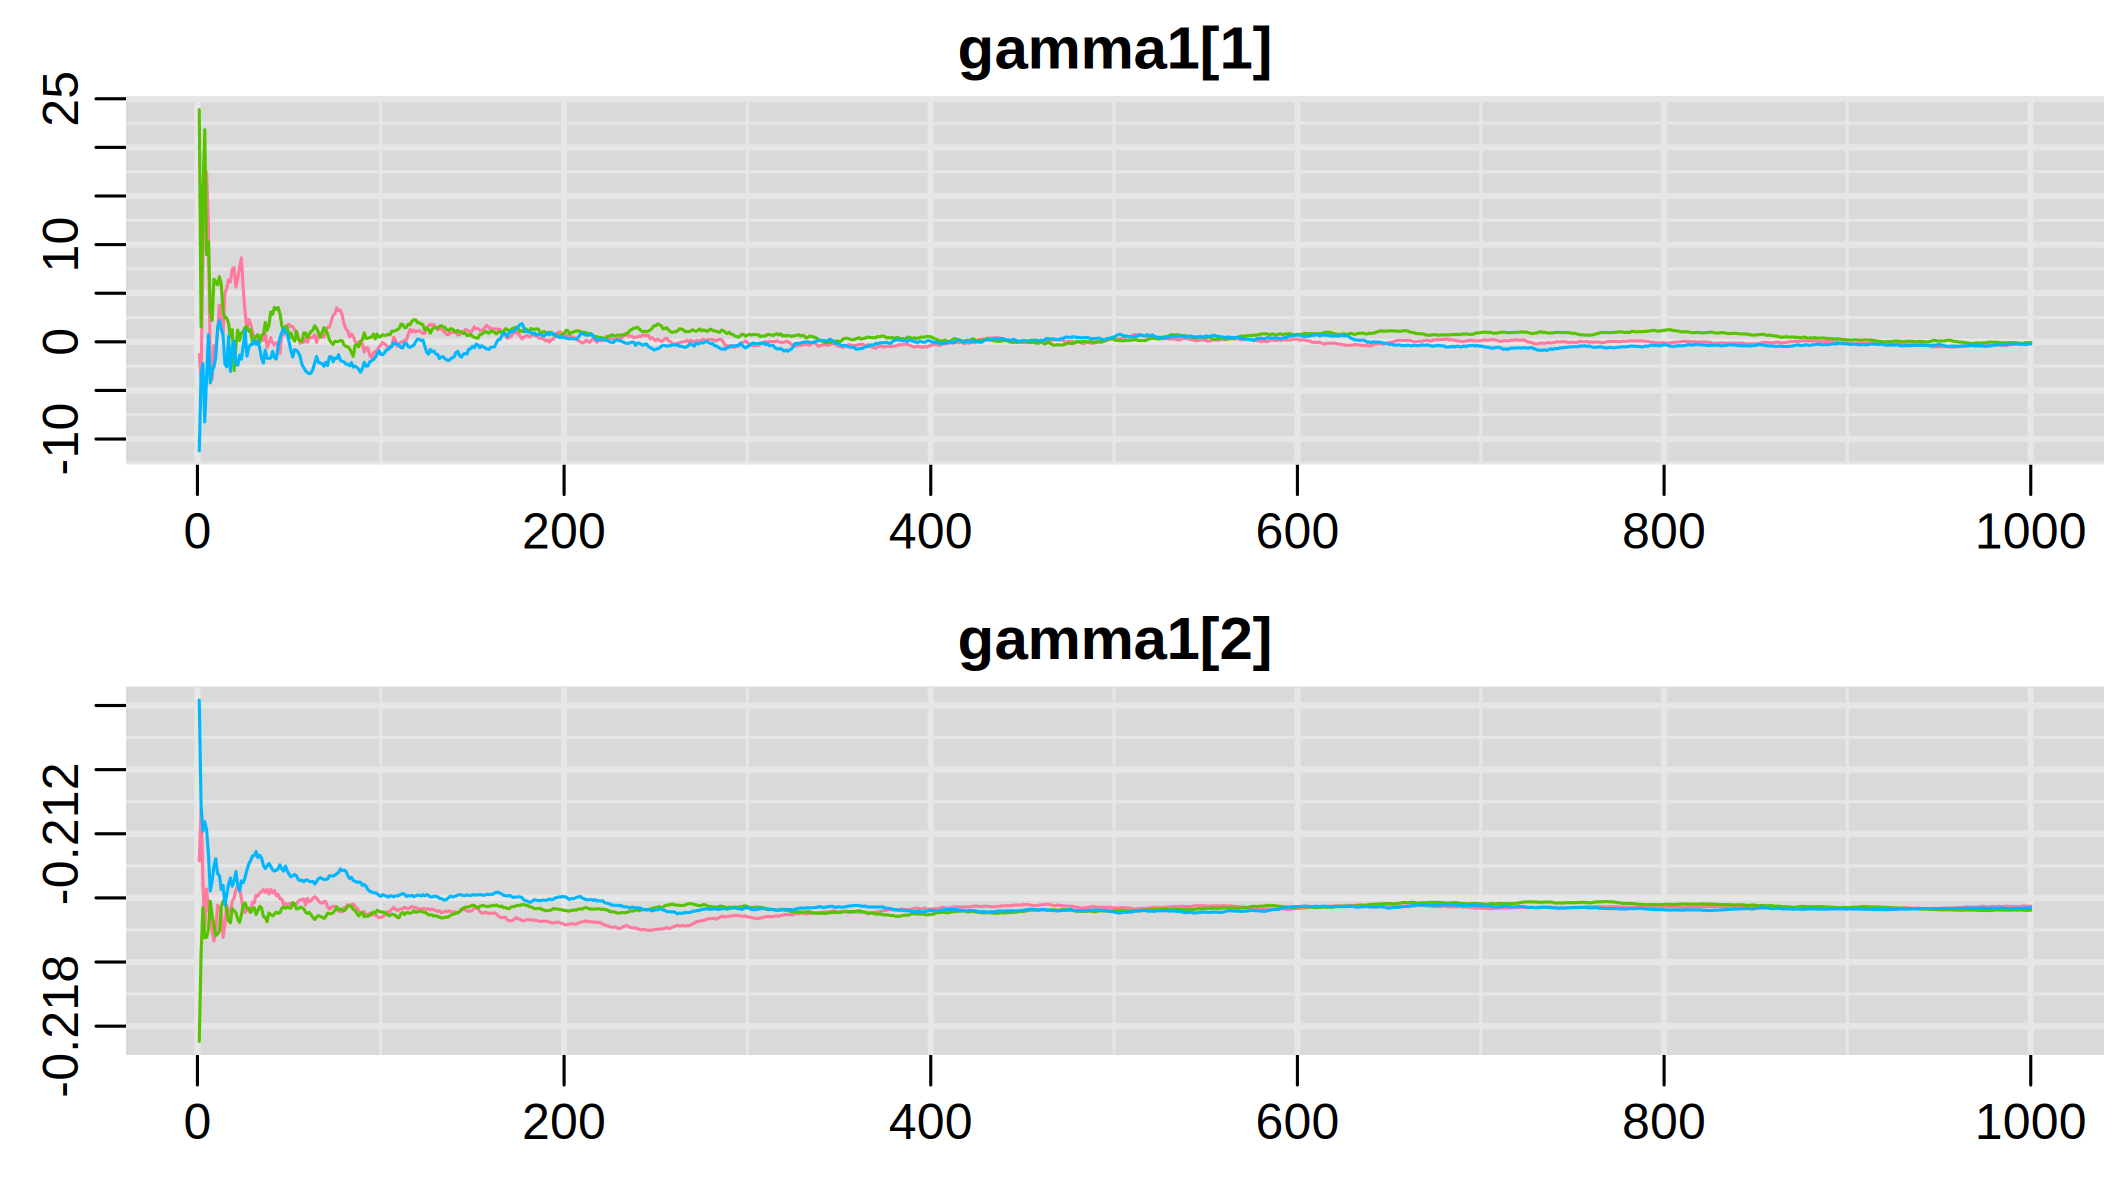
\includegraphics[width=\linewidth]{pictures/mod2/mod2rmean_gamma.png}
        %\caption{pi[41:60]}
        %\label{fig:sub2_1}
    \end{subfigure}
    %\hfill
    \begin{subfigure}{0.45\textwidth}
        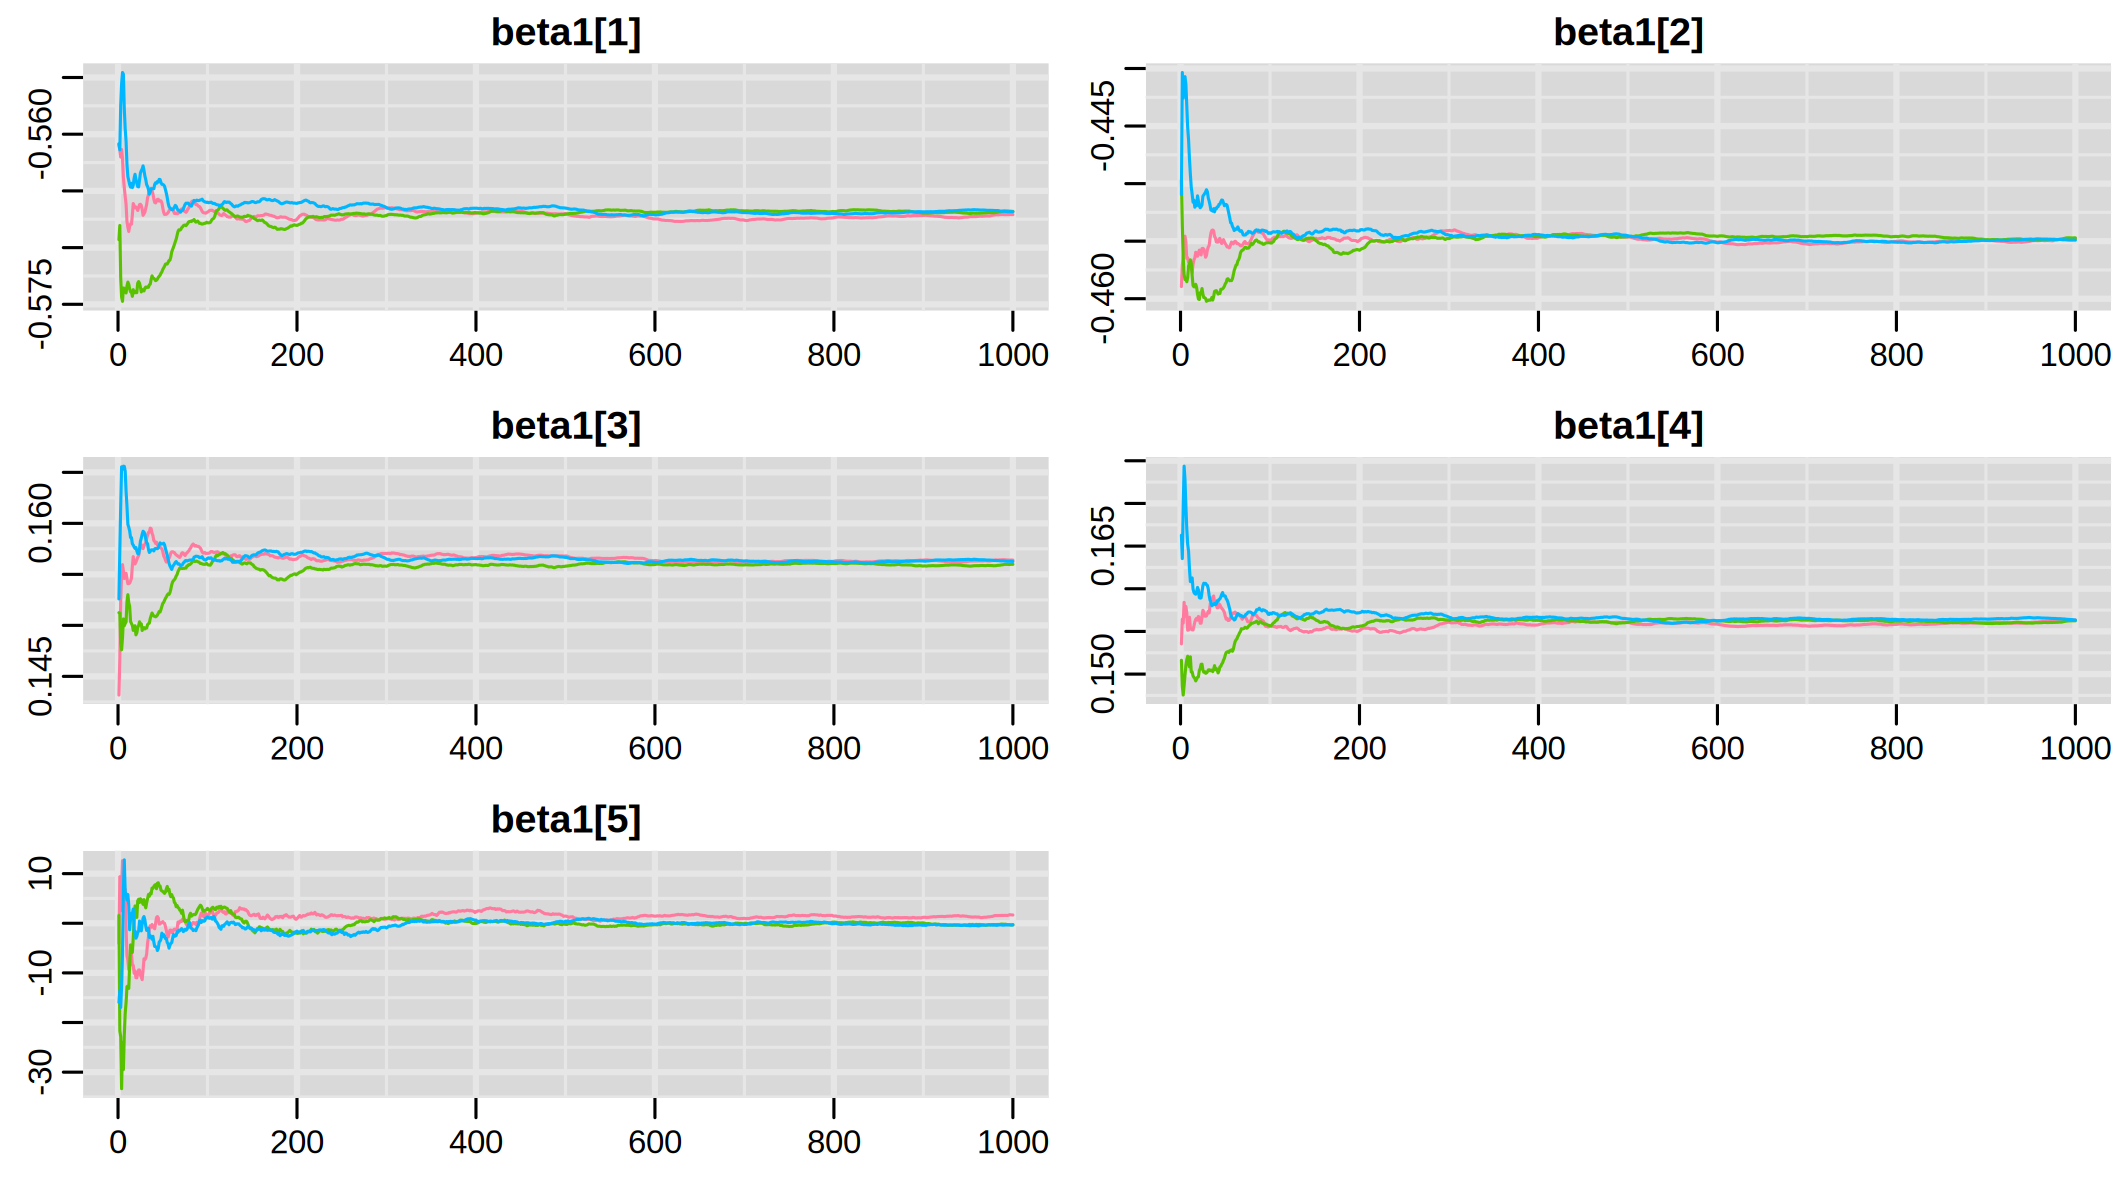
\includegraphics[width=\linewidth]{pictures/mod2/mod2rmean_beta.png}
        %\caption{pi[61:80]}
        %\label{fig:sub2_2}
    \end{subfigure}
    
    \caption{Sample running-mean plots for $\beta$, $\gamma$, $\sigma$ and $\mu$}
    \label{fig:runningmeanM2}
\end{figure}
\FloatBarrier % Ensures the figure doesn't float past this point

\textbf{Geweke diagnostic}: With the dynamic version of the Geweke diagnostic, the Z-values for $\beta$, $\gamma$, $\sigma$ (except in chain 1), $\alpha$ and $\pi_{iag}$ in all chains  fell inside the [-1.96, 1.96] interval indicating stationarity. Some of the Geweke diagnostic plots are shown in figure \ref{fig:gewekem2}. 

\begin{figure}[h!]
    \centering
    % First row
    \begin{subfigure}{0.45\textwidth}
        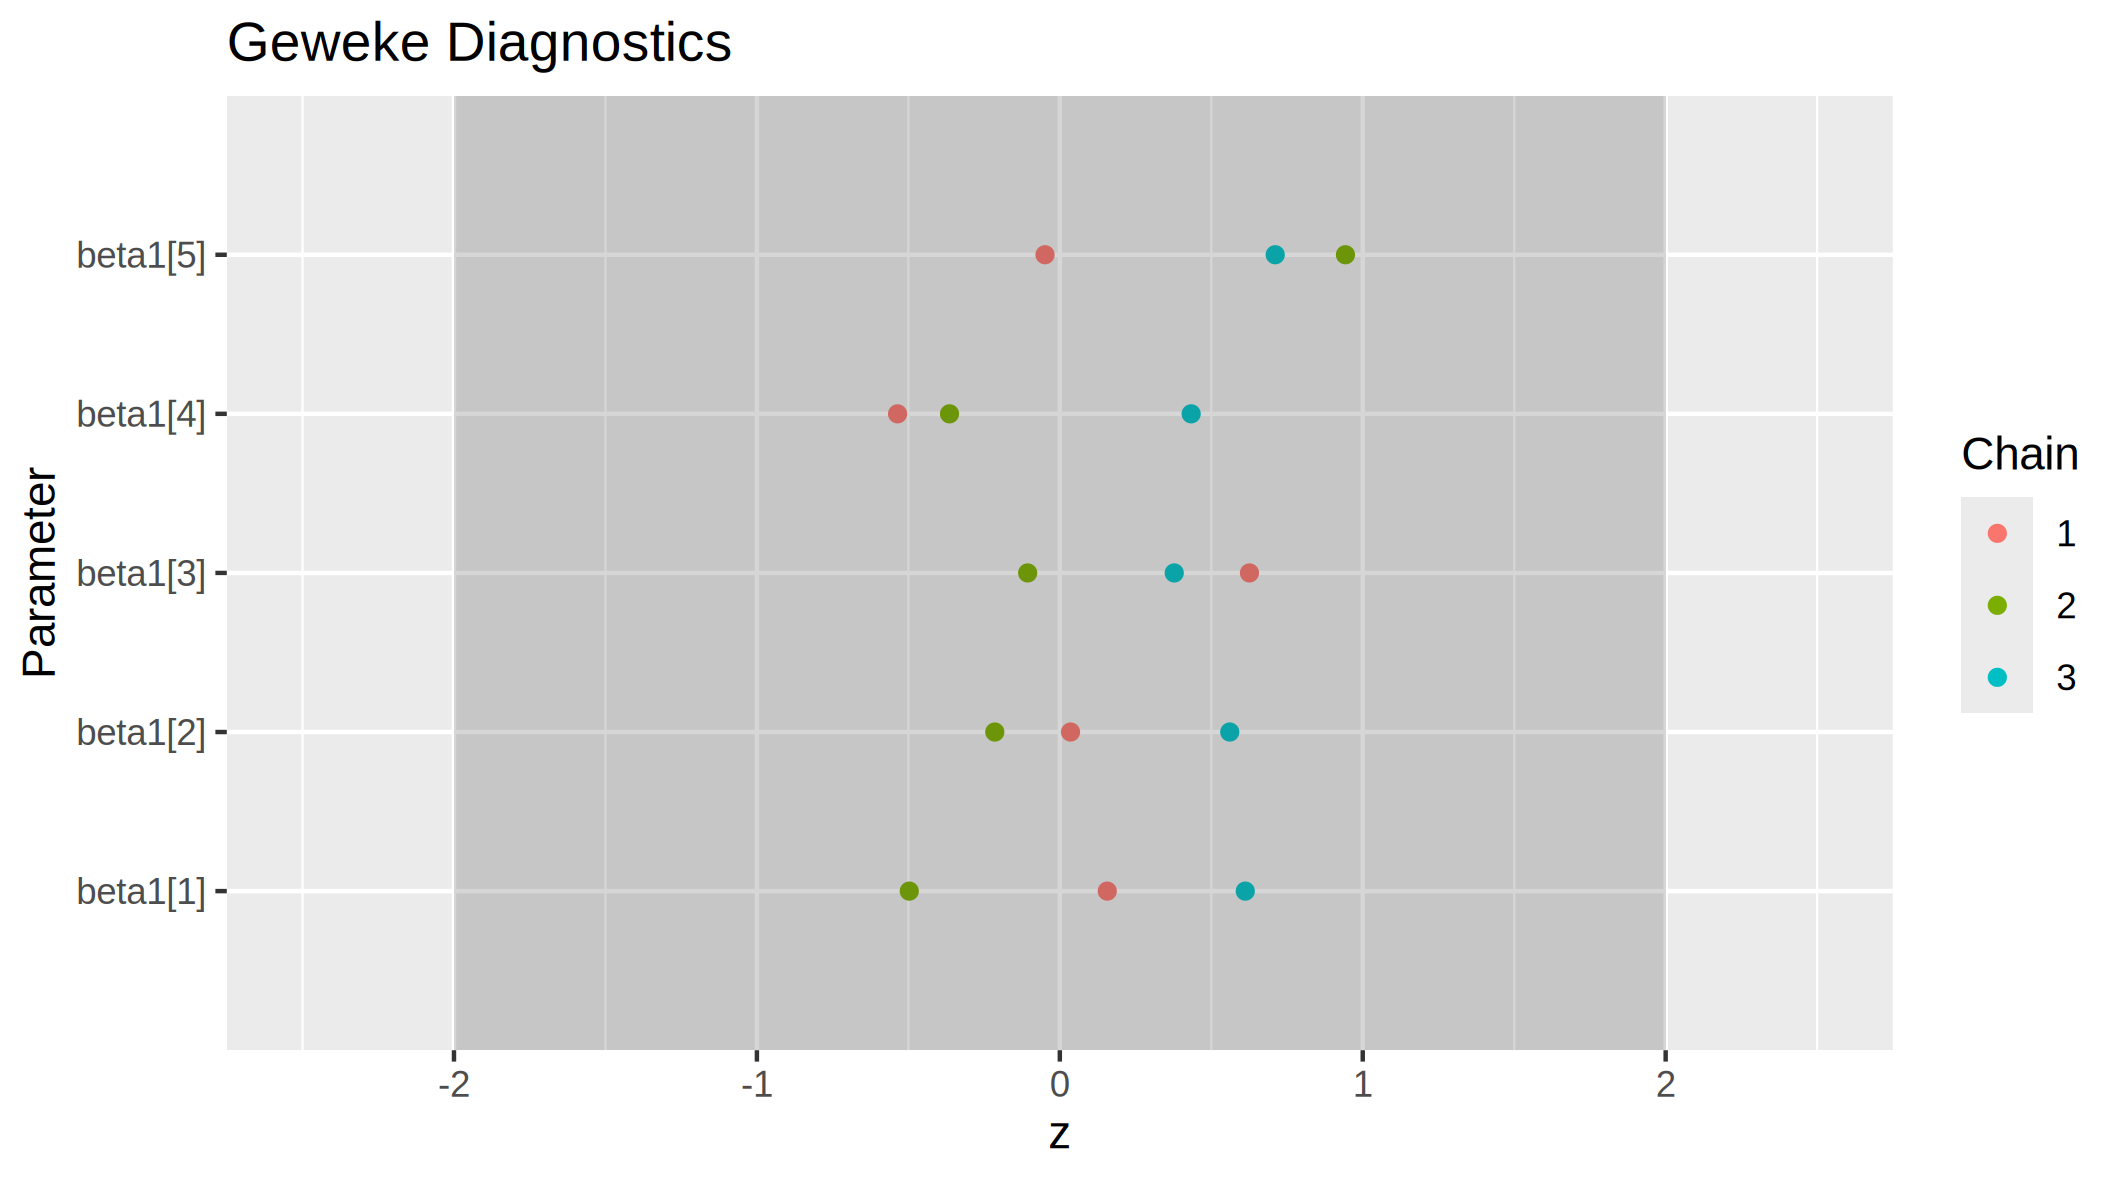
\includegraphics[width=\linewidth]{pictures/mod2/mod2geweke_beta.png}
        %\caption{pi[1:20]}
        %\label{fig:sub1_1}
    \end{subfigure}
    %\hfill
    \begin{subfigure}{0.45\textwidth}
        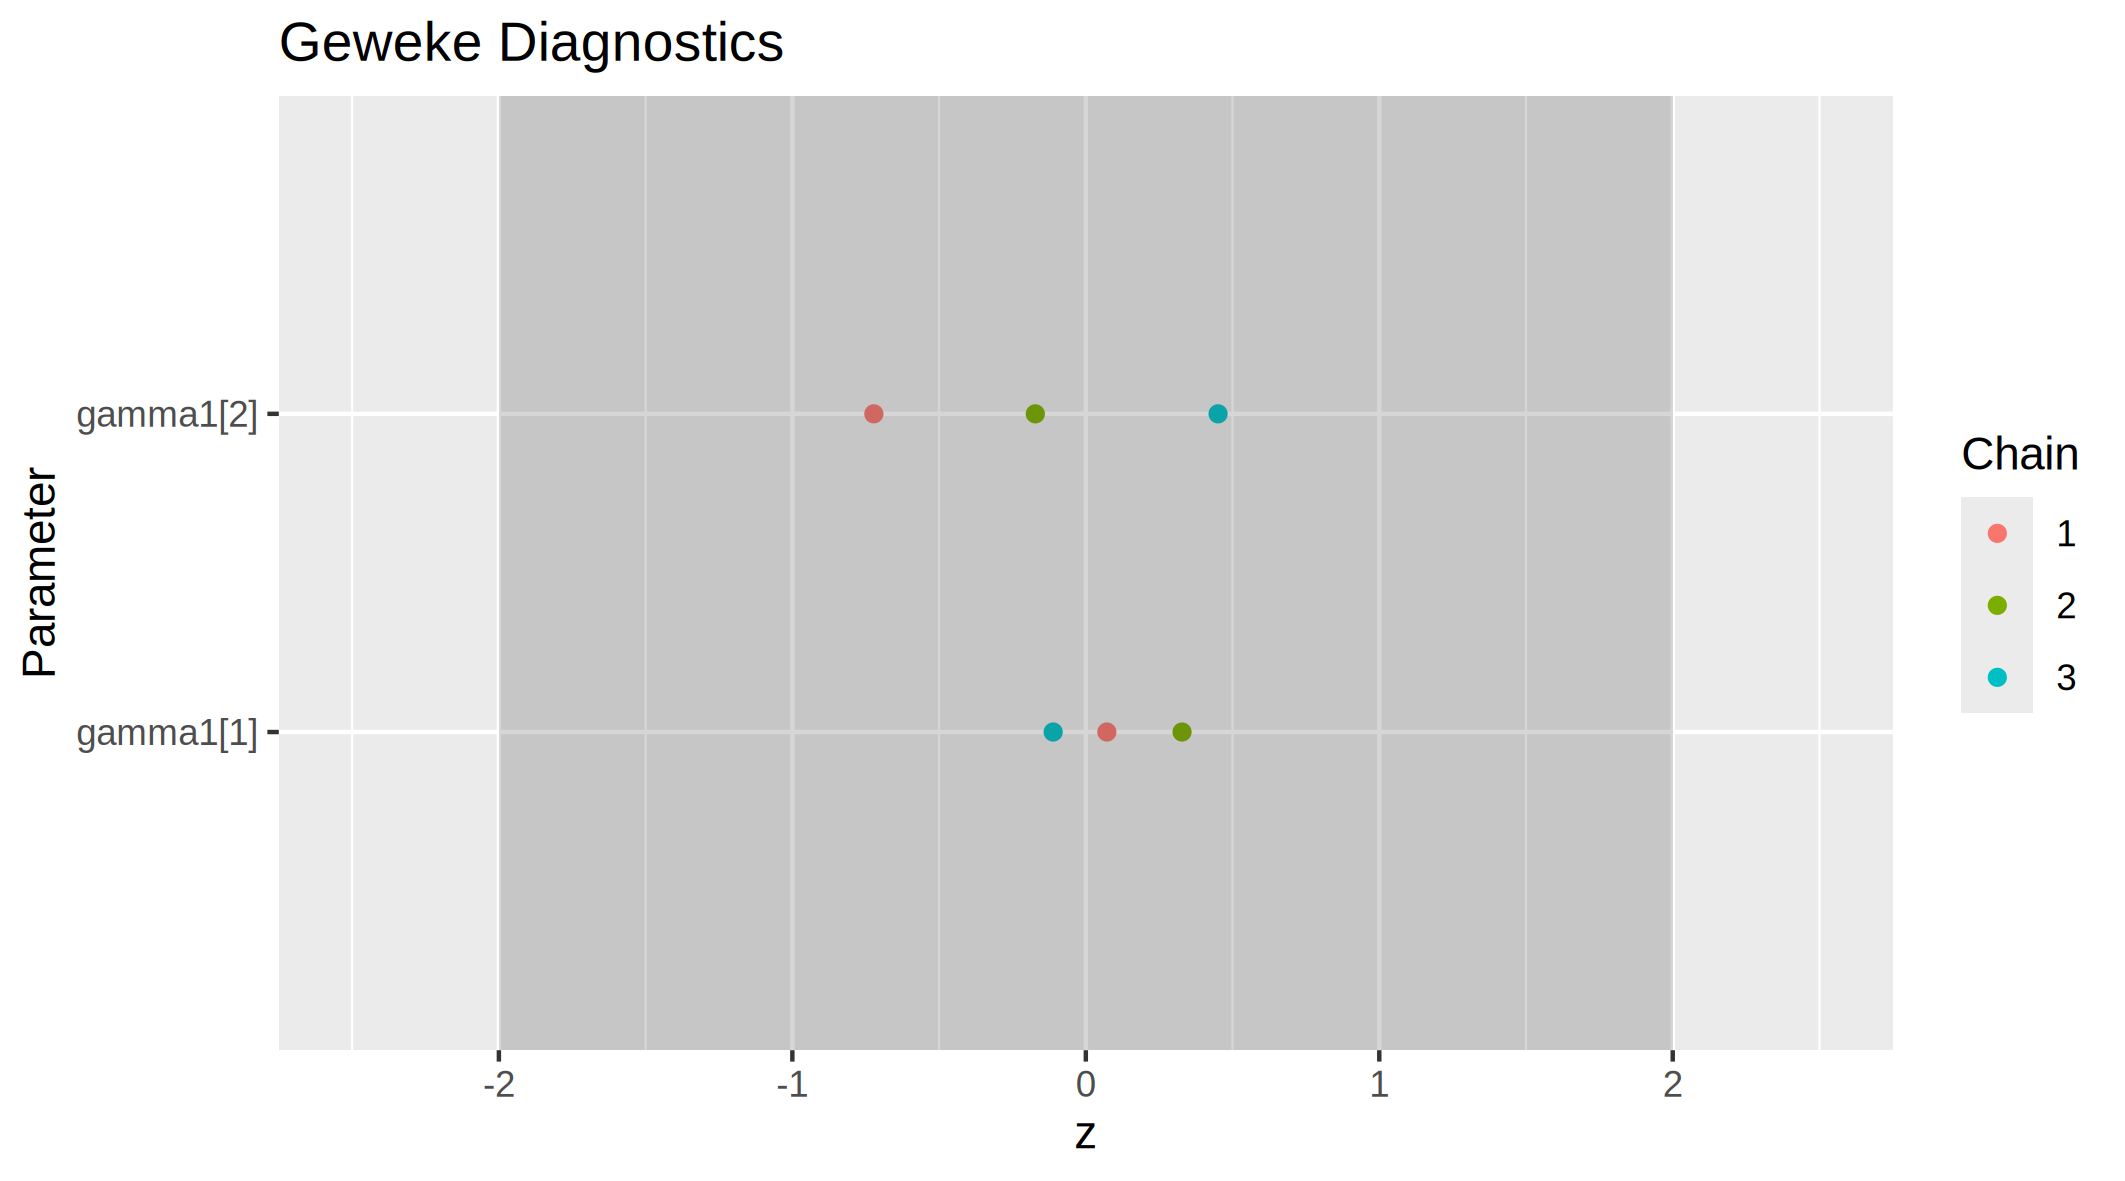
\includegraphics[width=\linewidth]{pictures/mod2/mod2geweke_gamma.png}
        %\caption{pi[21:40]}
        %\label{fig:sub1_2}
    \end{subfigure}

    % Second row
    \vskip\baselineskip
    \begin{subfigure}{0.45\textwidth}
        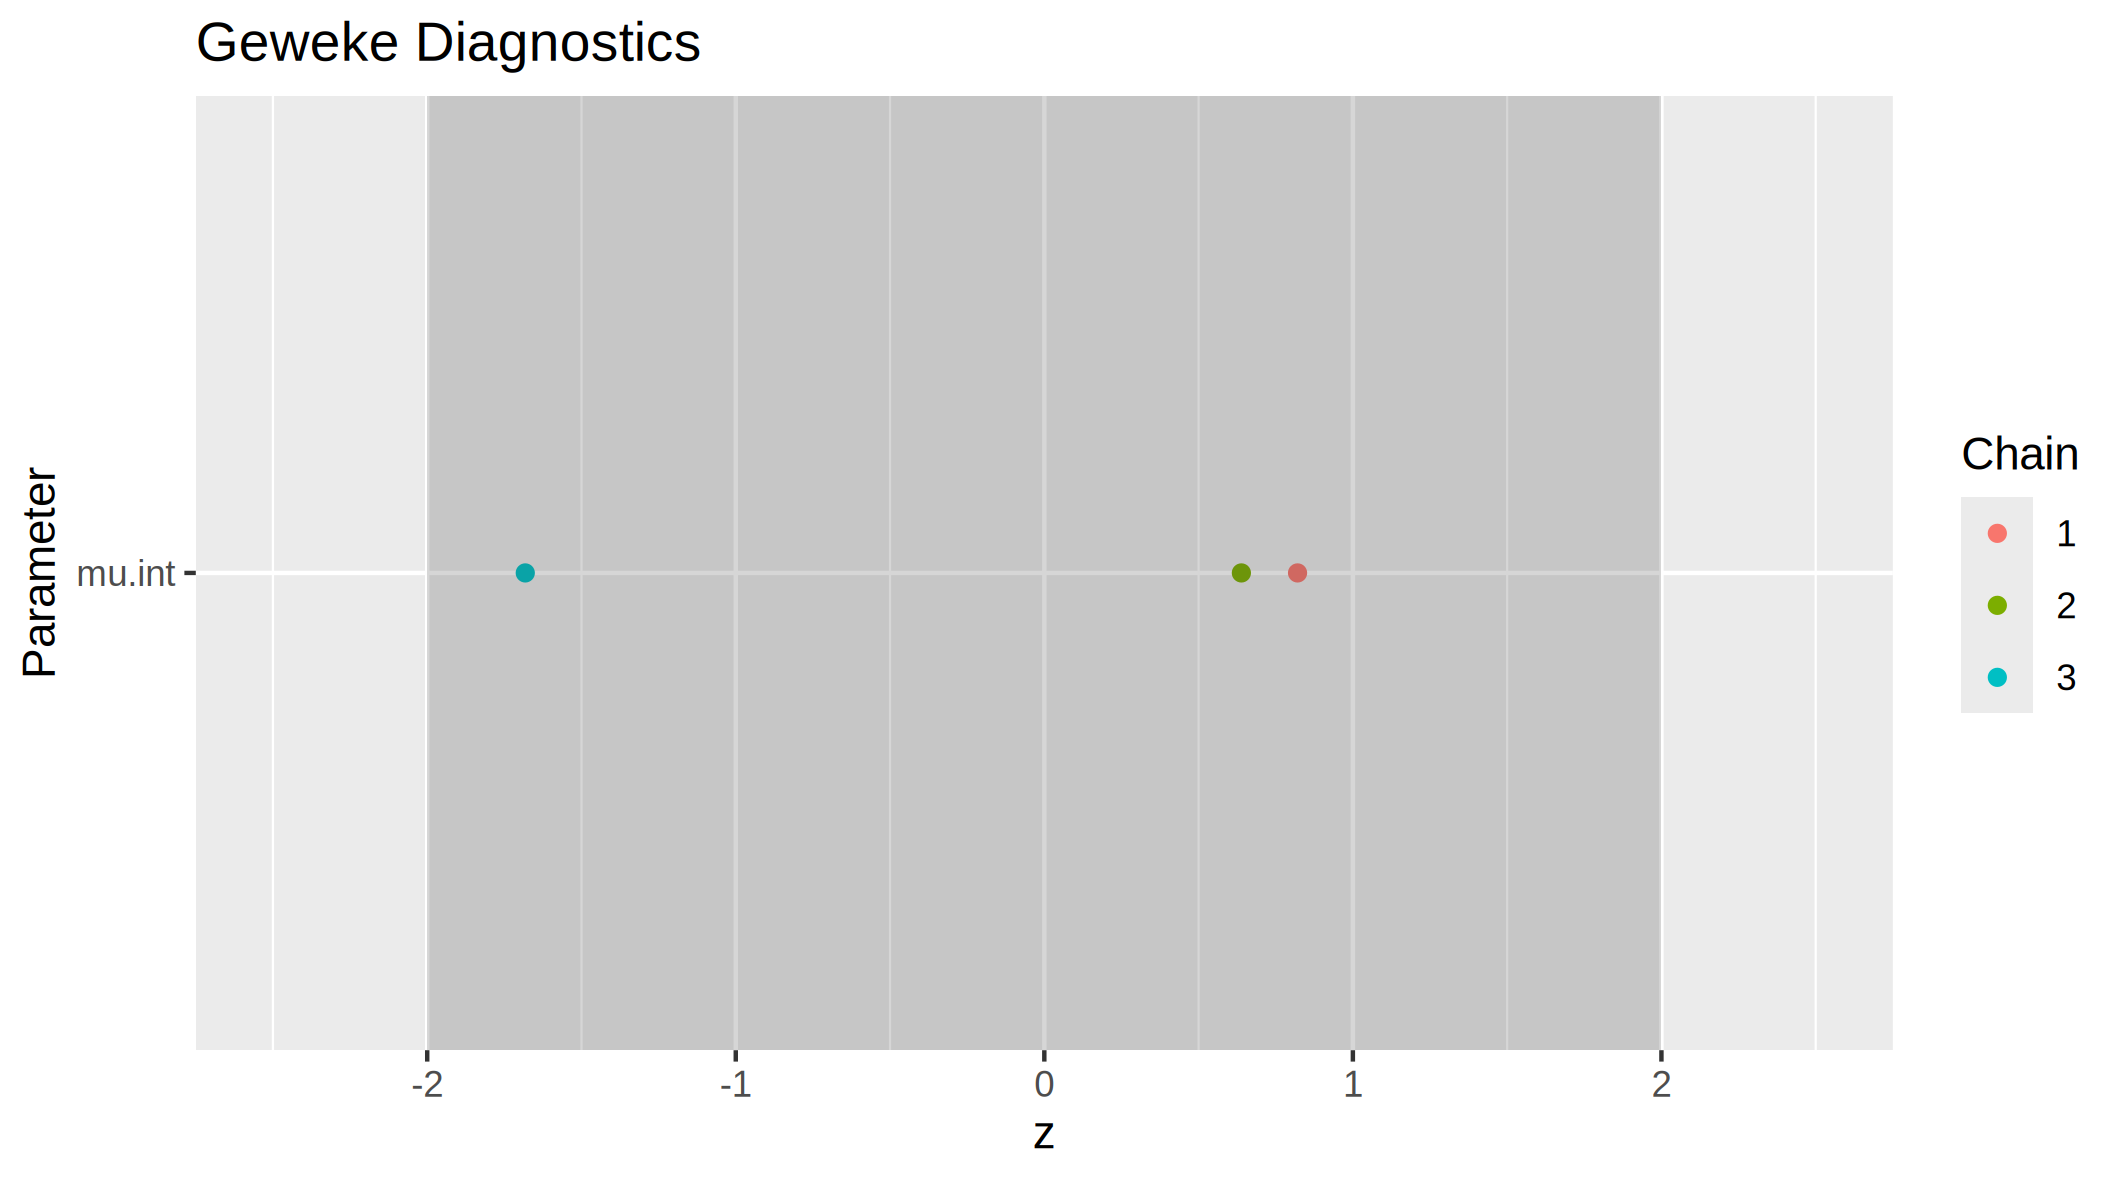
\includegraphics[width=\linewidth]{pictures/mod2/mod2geweke_muint.png}
        %\caption{pi[41:60]}
        %\label{fig:sub2_1}
    \end{subfigure}
    %\hfill
    \begin{subfigure}{0.45\textwidth}
        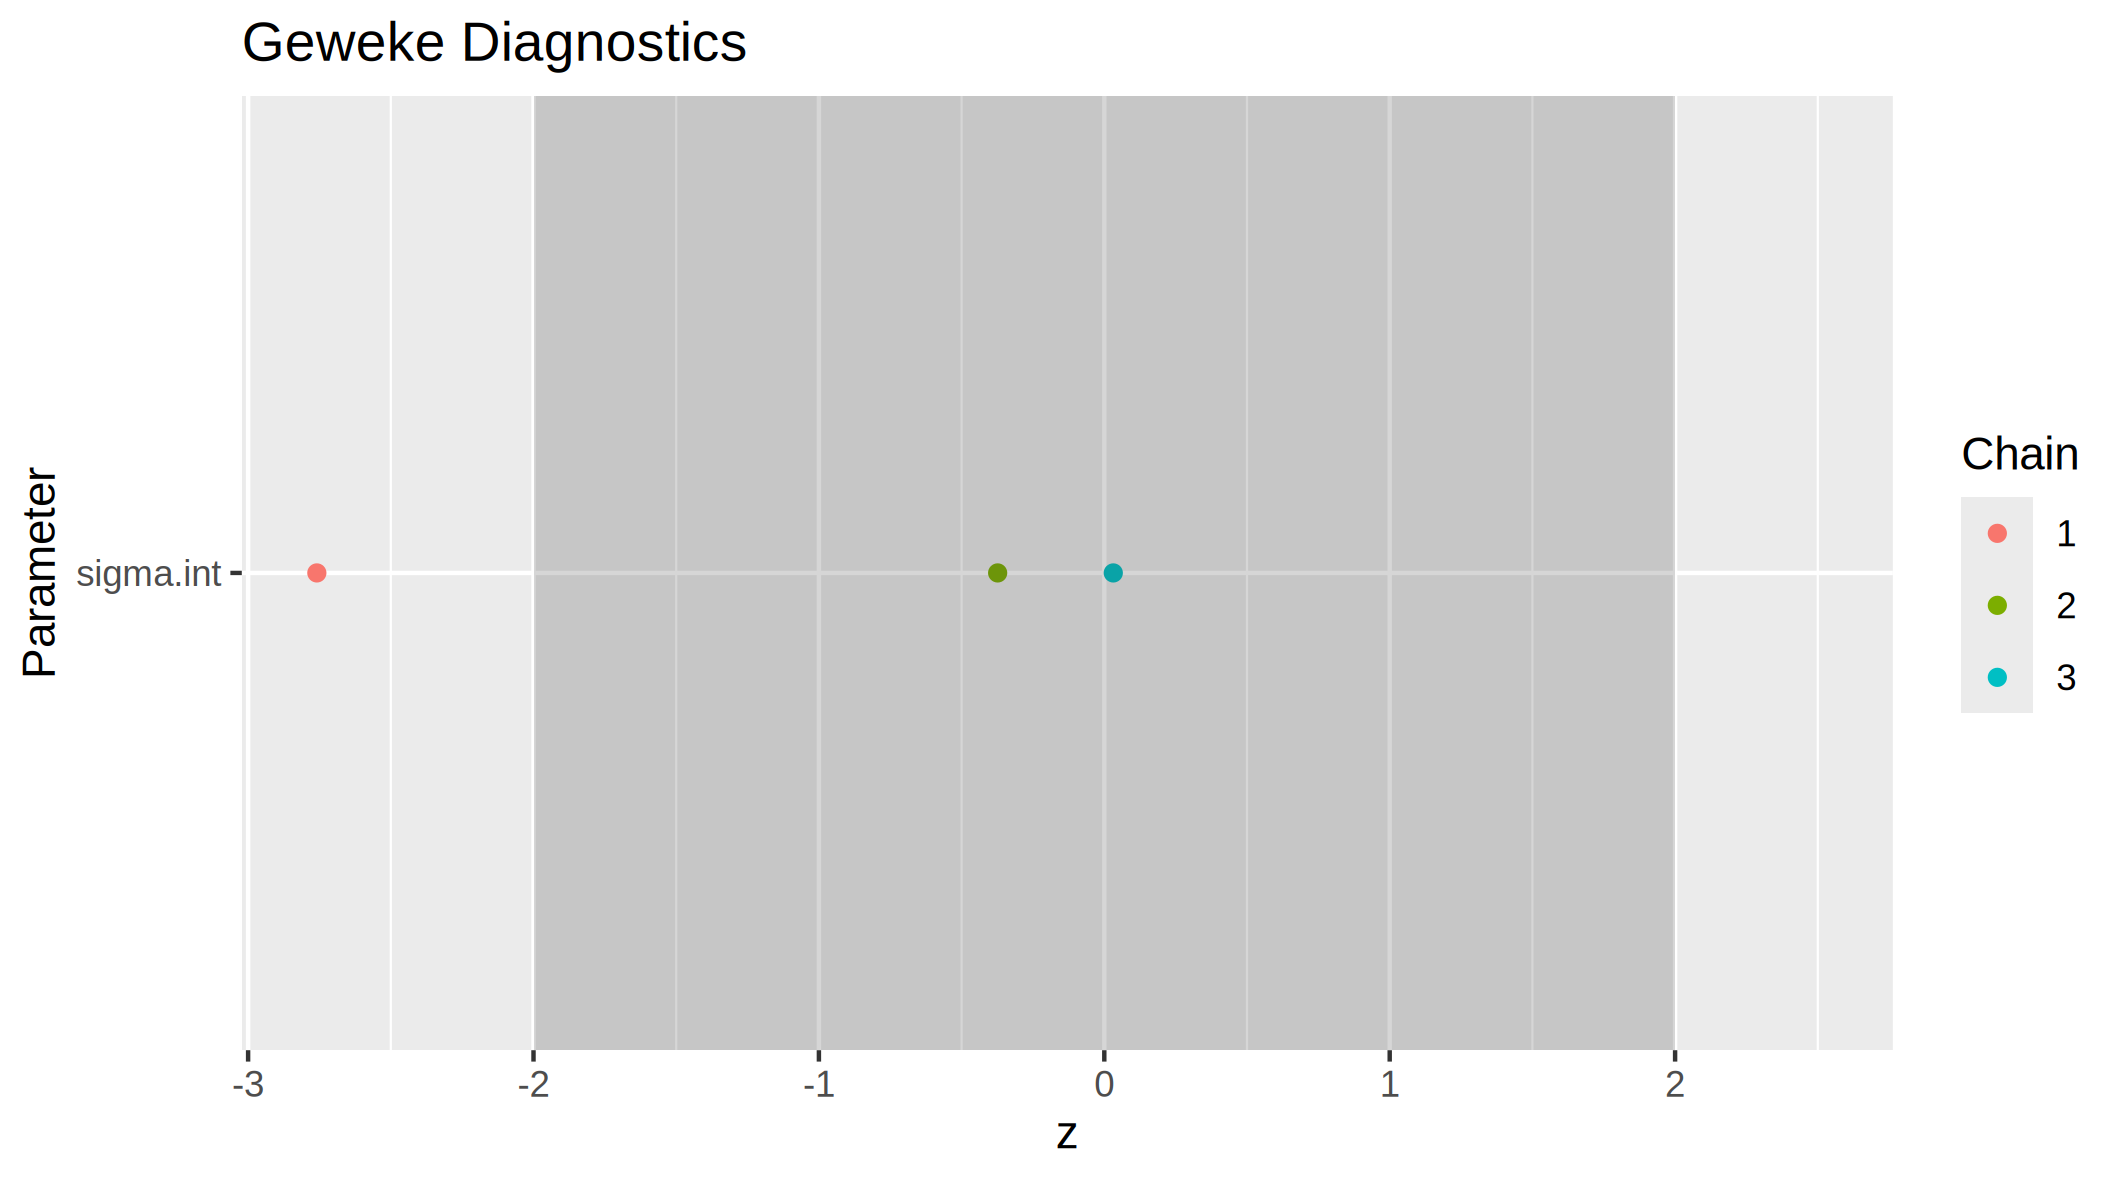
\includegraphics[width=\linewidth]{pictures/mod2/mod2geweke_sigmaint.png}
        %\caption{pi[61:80]}
        %\label{fig:sub2_2}
    \end{subfigure}
    
    \caption{Geweke diagnostic for $\beta$, $\gamma$, $\sigma$ and $\mu$}
    \label{fig:gewekem2}
\end{figure}
\FloatBarrier

\textbf{Brooks–Gelman–Rubin (BGR) diagnostic}: With the dynamic version of the GR interval diagnostics shown in figure \ref{fig:gewekem2}, the curves stabilized almost immediately for all parameters ($\beta$, $\gamma$, $\sigma$, $\mu$ and $\pi_{iag}$) and no additional iterations appeared necessary. Convergence was not rejected with the Gelman and Rubin's convergence diagnostic. The potential scale reduction factor (psrf), $\hat{R_c}$ = 1 for all these parameters. 

\begin{figure}[h!]
    \centering
    % First row
    \begin{subfigure}{0.45\textwidth}
        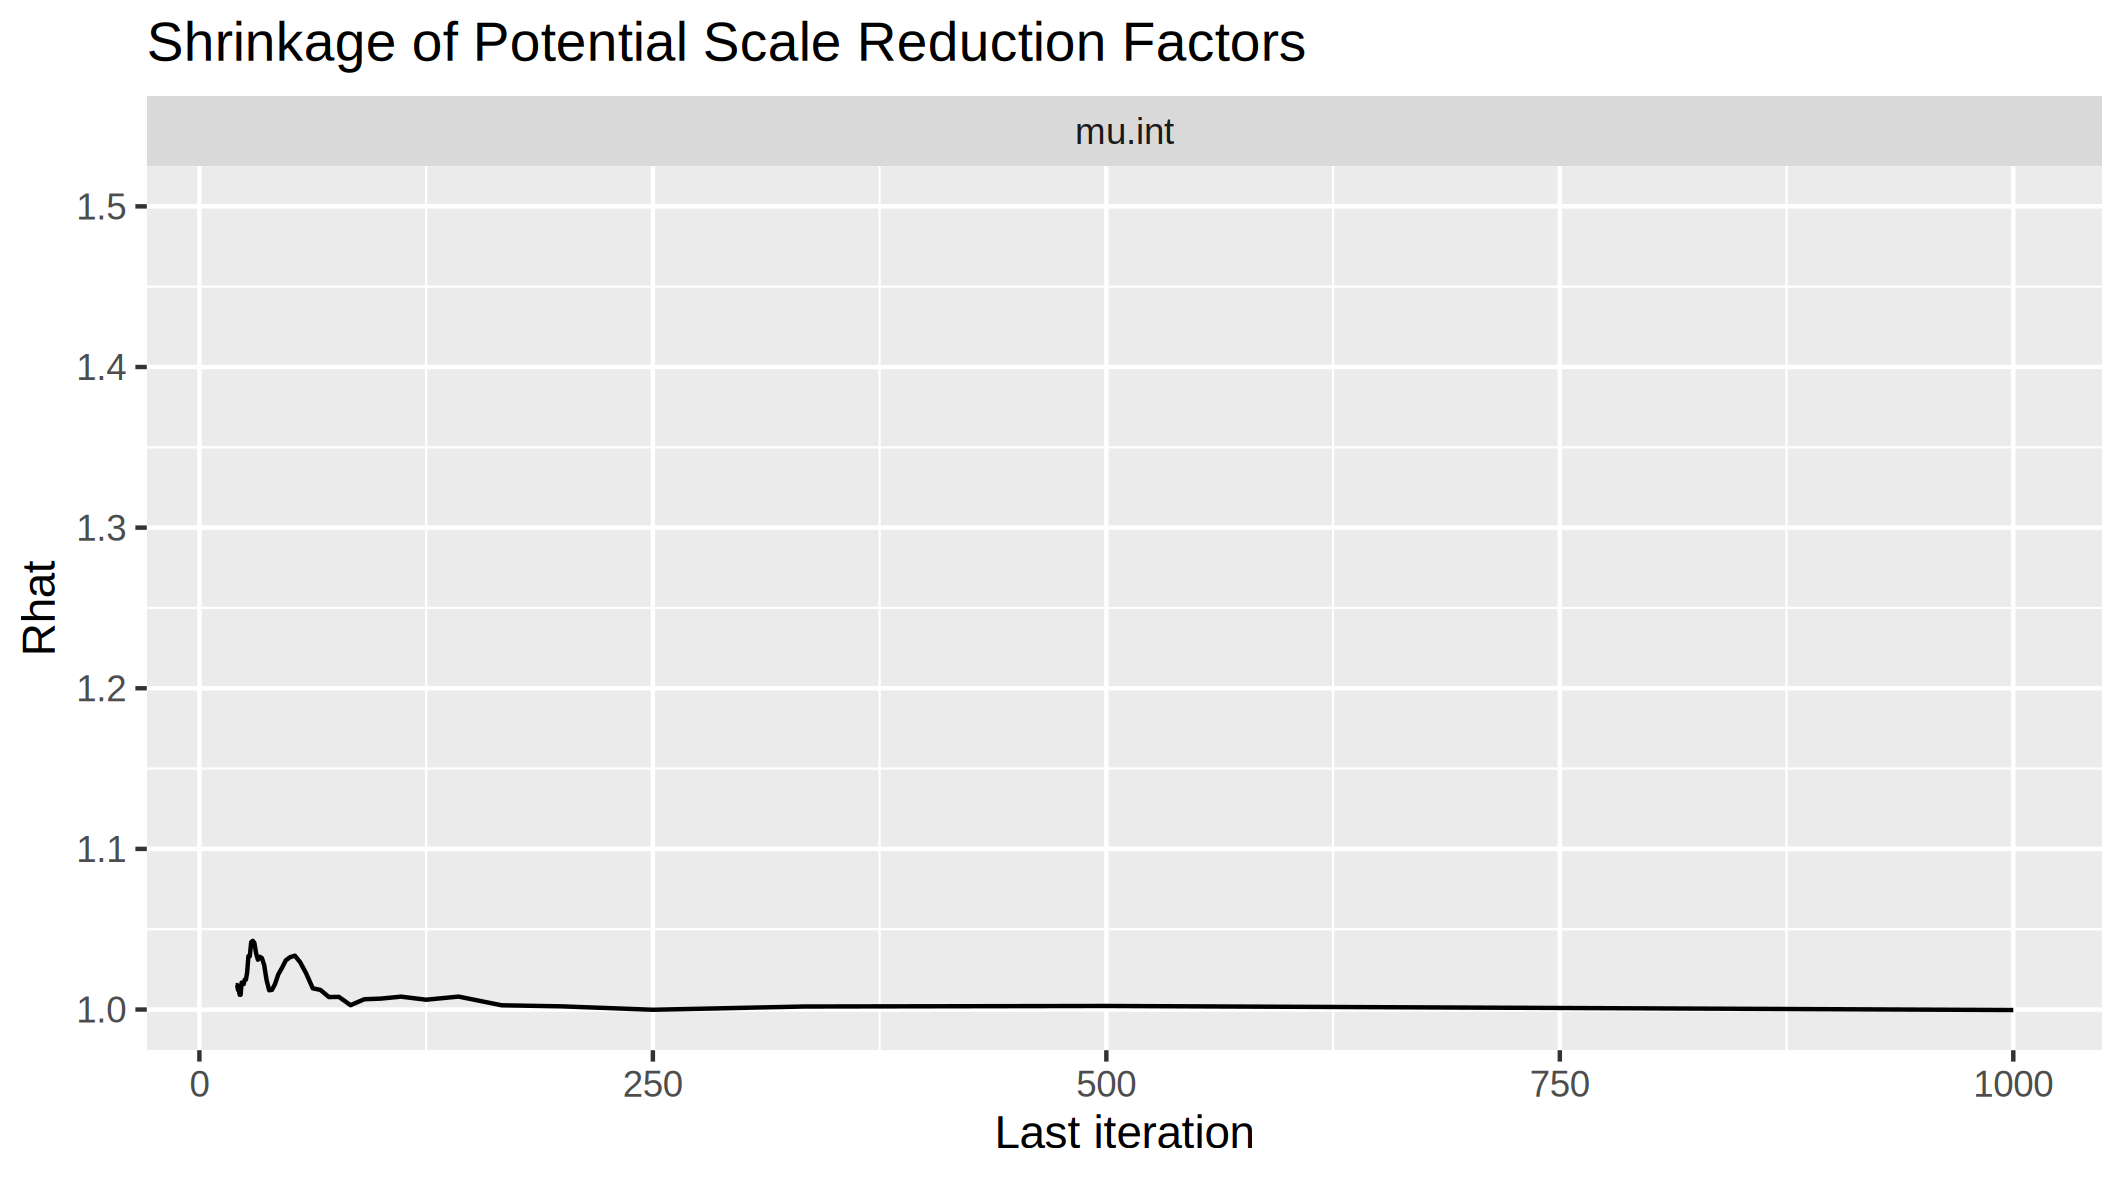
\includegraphics[width=\linewidth]{pictures/mod2/mod2gbr_muint.png}
        %\caption{pi[1:20]}
        %\label{fig:sub1_1}
    \end{subfigure}
    %\hfill
    \begin{subfigure}{0.45\textwidth}
        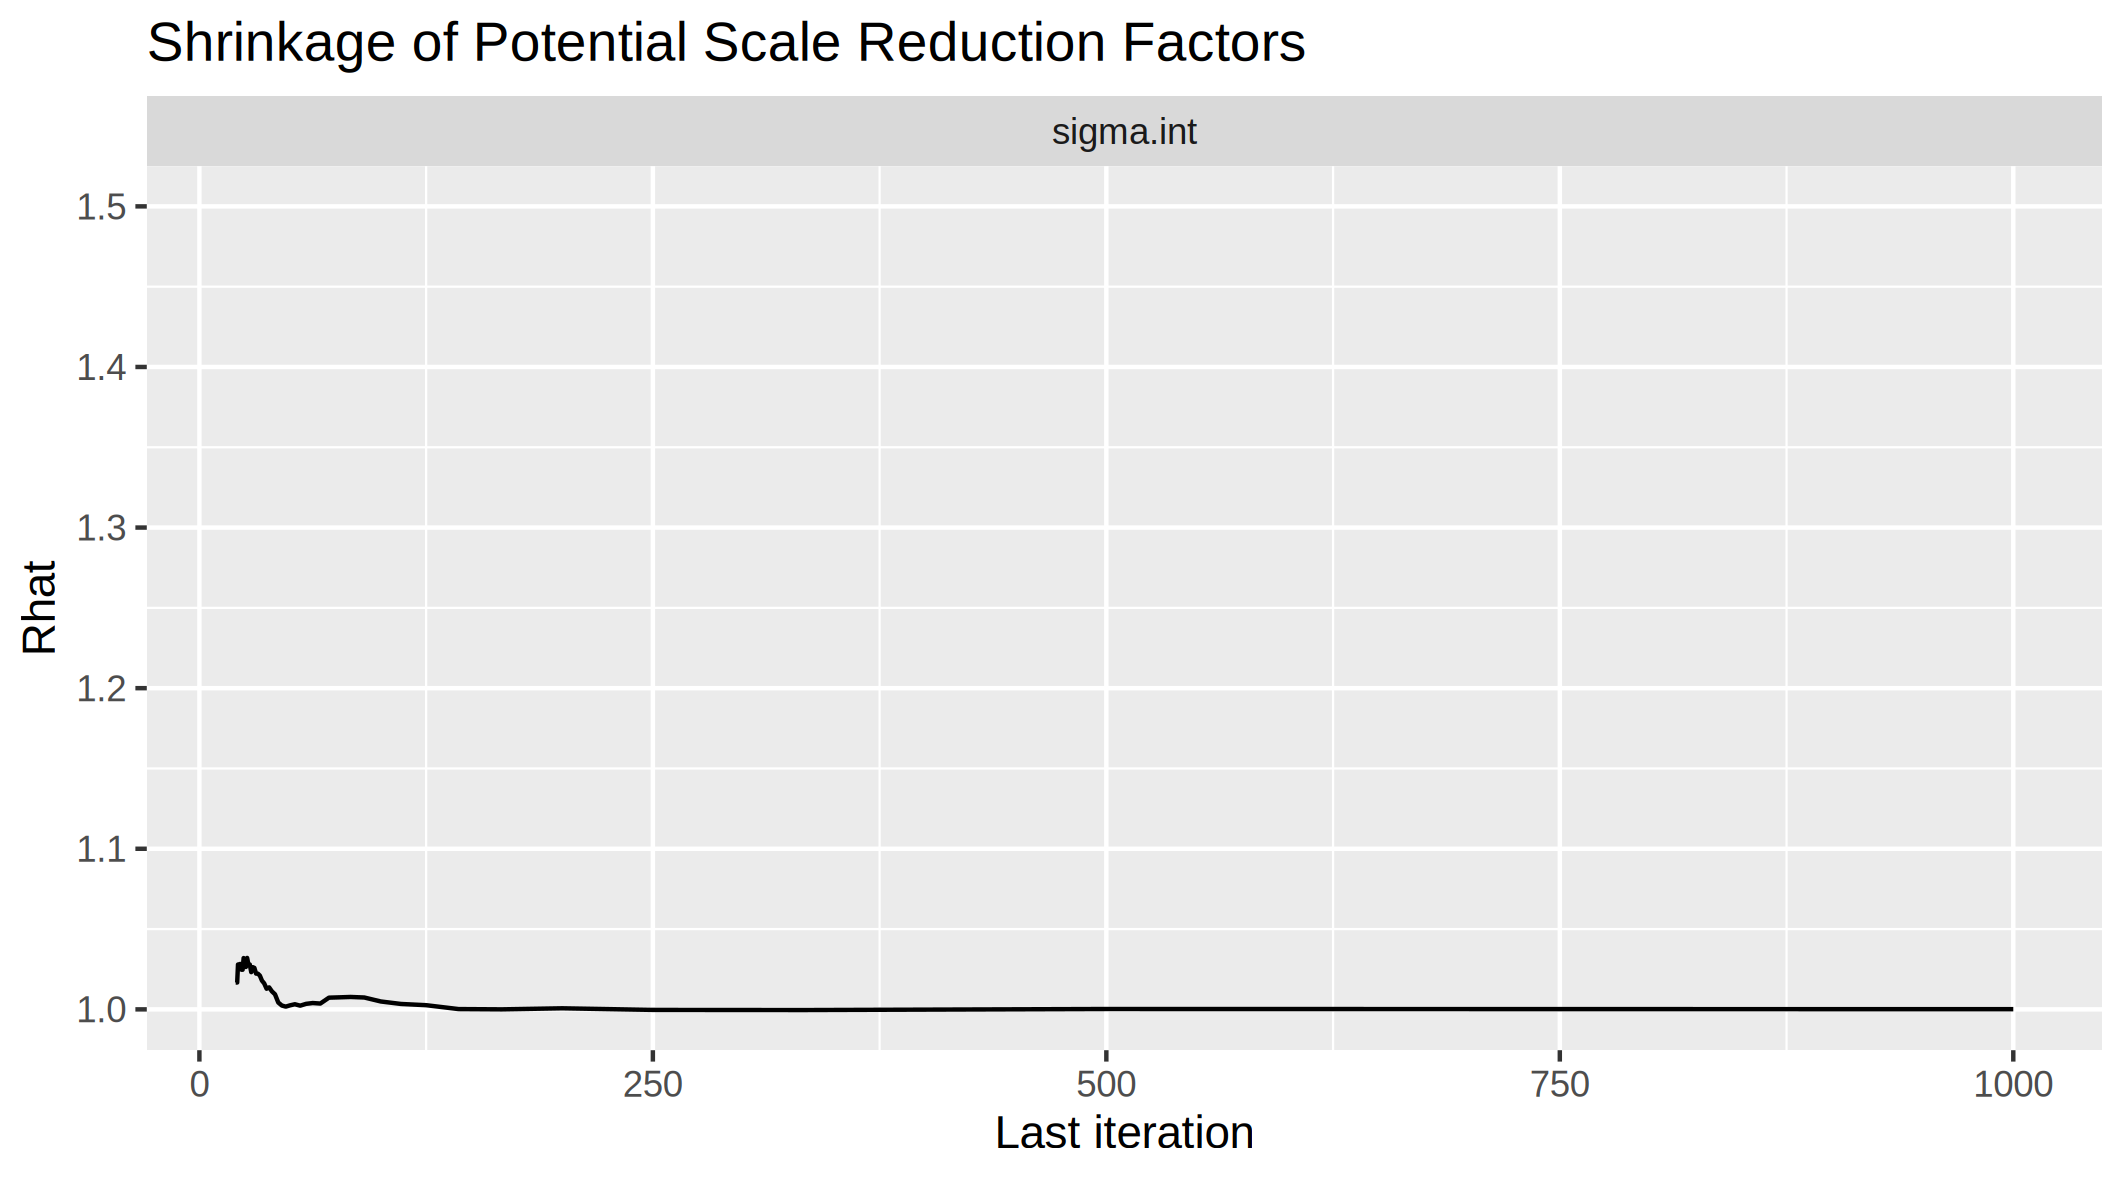
\includegraphics[width=\linewidth]{pictures/mod2/mod2gbr_sigmaint.png}
        %\caption{pi[21:40]}
        %\label{fig:sub1_2}
    \end{subfigure}

    % Second row
    \vskip\baselineskip
    \begin{subfigure}{0.45\textwidth}
        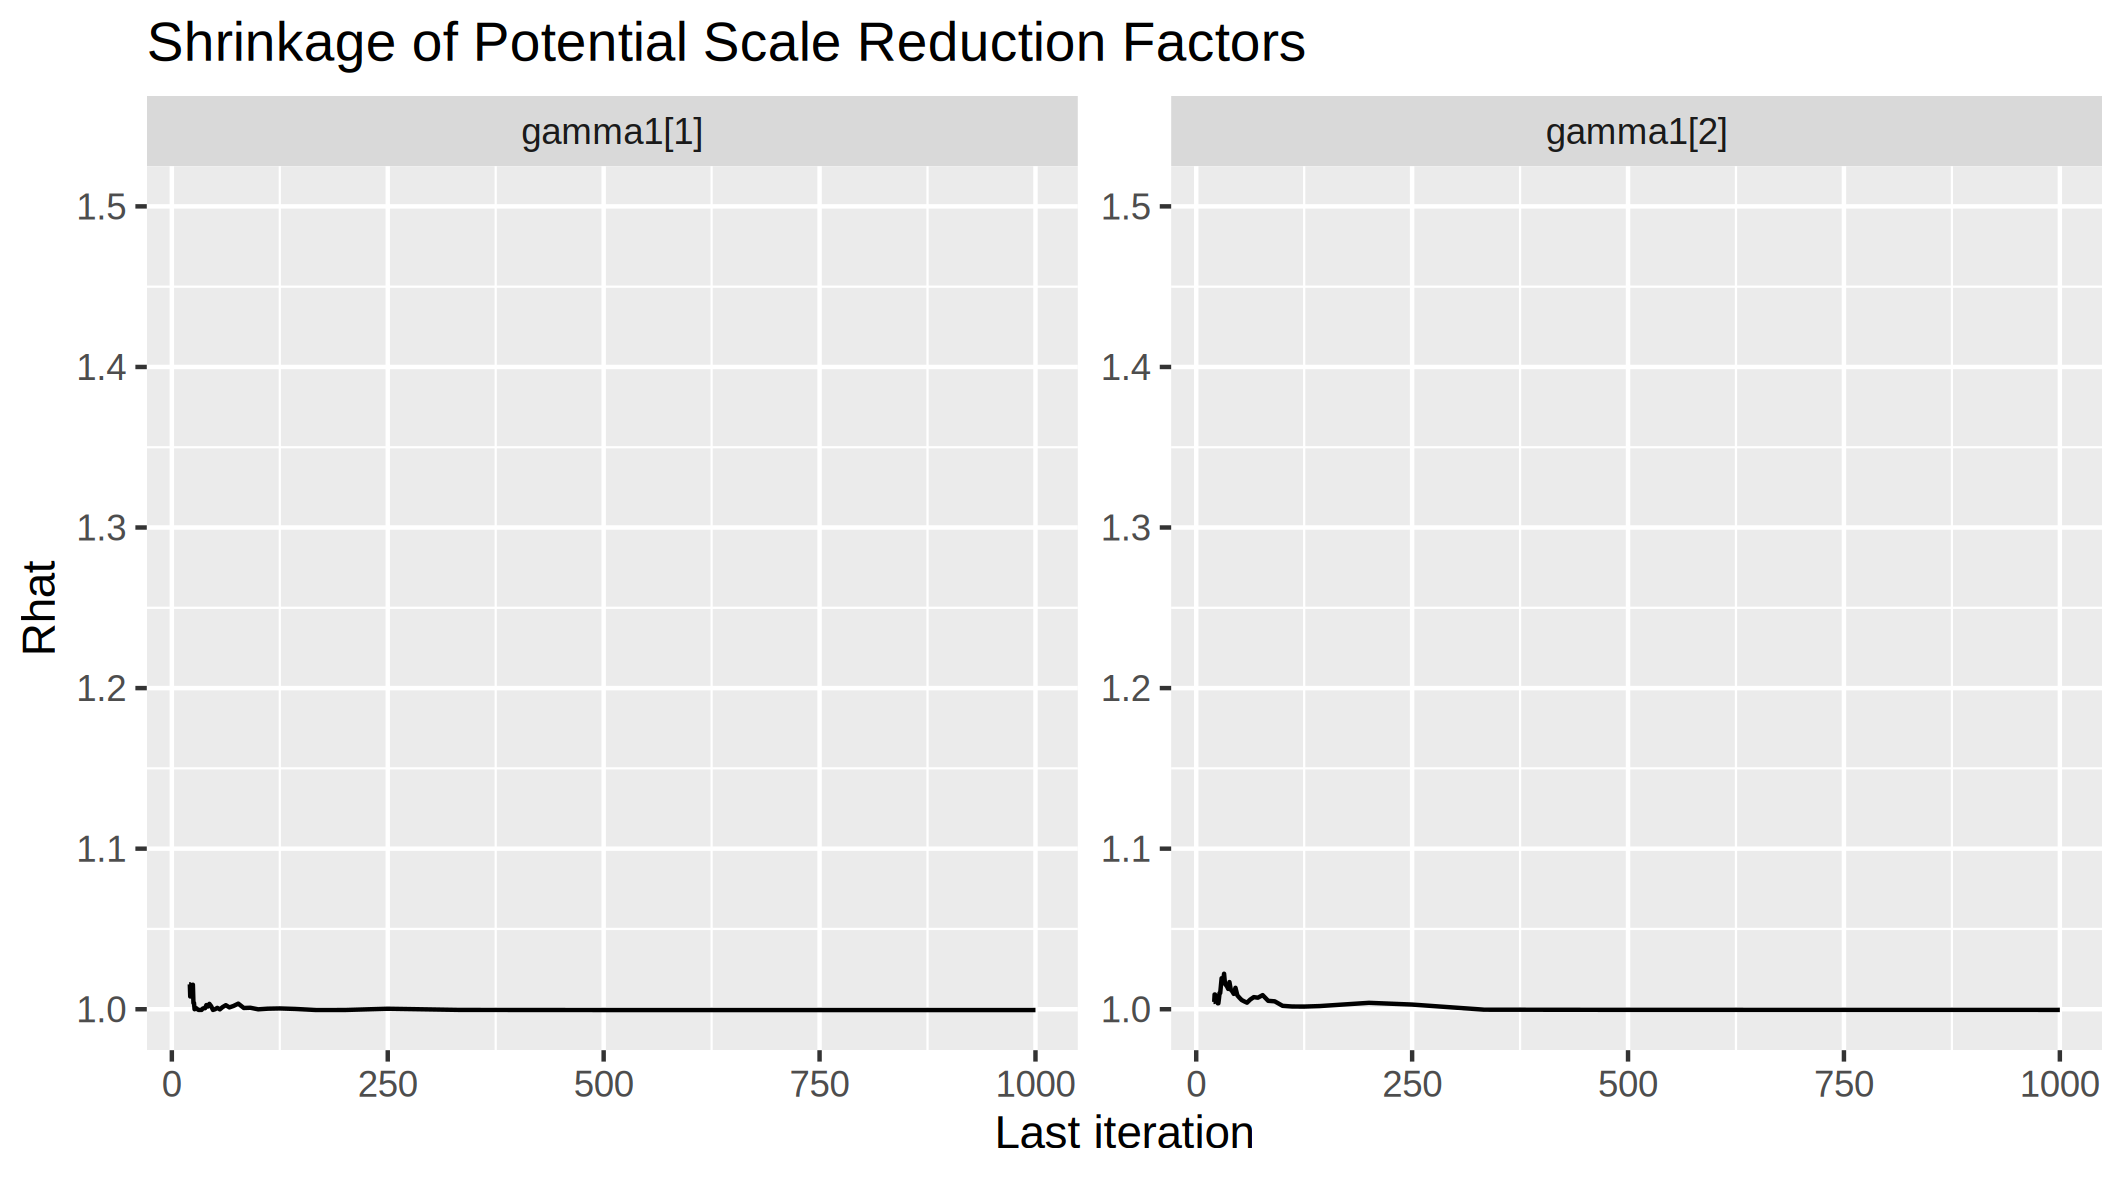
\includegraphics[width=\linewidth]{pictures/mod2/mod2gbr_gamma.png}
        %\caption{pi[41:60]}
        %\label{fig:sub2_1}
    \end{subfigure}
    %\hfill
    \begin{subfigure}{0.45\textwidth}
        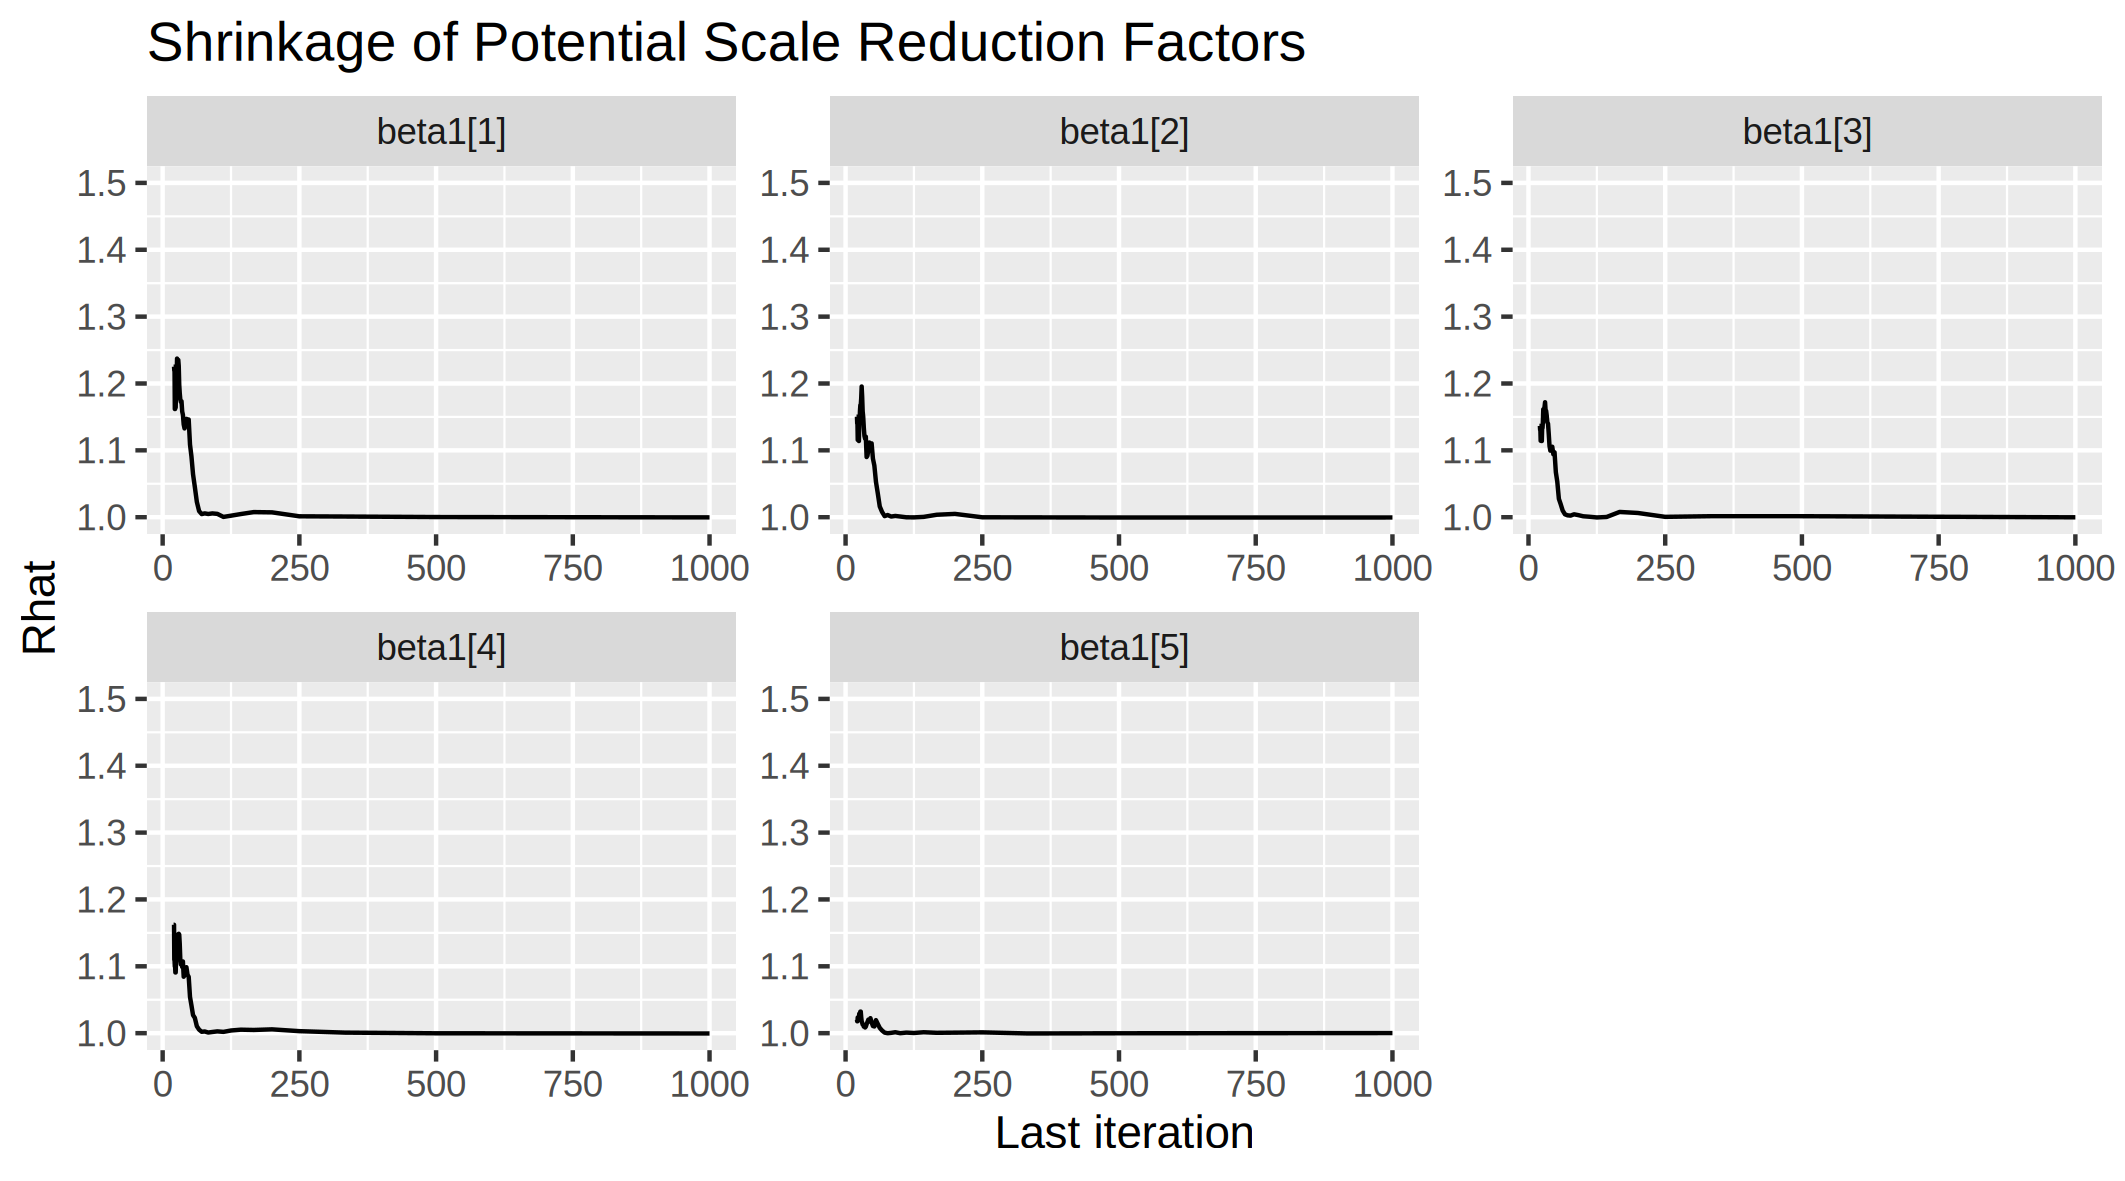
\includegraphics[width=\linewidth]{pictures/mod2/mod2gbr_beta.png}
        %\caption{pi[61:80]}
        %\label{fig:sub2_2}
    \end{subfigure}
    
    \caption{Sample Gelman-Rubin-Brooks plots for $\beta$, $\gamma$, $\sigma$ and $\mu$}
    \label{fig:GRBm2}
\end{figure}
\FloatBarrier % Ensures the figure doesn't float past this point

\textbf{Heidelberger–Welch (HW) diagnostic}: The Heidelberger–Welch tests, that is, stationarity test as well as the halfiwidth test were passed for $\beta$, $\gamma$, $\sigma$ and $\mu$ parameters and almost all $\pi_{iag}$ except a few. Further iterations did not make any change on the $\pi_{iag}$ with failed tests.

\textbf{Raftery–Lewis (RL) diagnostic}: The dependence factor for all parameters was below 2 an indicator for independent sampling therefore signalling good convergence.

\subsubsection{What do you conclude from this model?}

After convergence, the estimated values for $\alpha$ = 0.329. For the age group effects, $\beta_1, \beta_2, \beta_3, \beta_4$ and  $\beta_5$ were -0.567, -0.458, 0.156, 0.156 and 0.348 respectively. This implies that the age groups 50-54 and 55-59 have a negative effect on the participation rate while the rest age groups have a positive effect on the participation rate. The estimates for the gender effects, $\gamma_1$ and $\gamma_2$ were -0.150 and -0.214 for male and females respectively.   

\subsubsection{For which regions and age-gender-groups is $P$ ($\pi_{iag}$ $<$ 0.30$|$Y ) $>$ 0.9?}
Similarly as in model 1, we explore the posterior probability that the true participation rate $\pi_{iag}$ for the $i$th region, $a$th age and $g$th gender is less than 0.30 given the observed data $Y$ and prior information. A high value of this probability as requested indicates strong evidence based on prior beliefs and data that the true parameter $\pi_{iag}$ lies below 0.30. A number of regions meet this criteria and their posterior probabilities are shown in table  
\ref{tab:posterior_pi2}. 


\begin{table}[h!]
    \centering
    \begin{threeparttable}
        \caption{Regions-age-gender-groups where $P$ ($\pi_{iag}$ $<$ 0.30$|$Y ) $>$ 0.9.}
        \label{tab:posterior_pi2}
        \begin{tabular}{cc|cc|cc}
        \hline
        \textbf{Parameter} & $P$ & \textbf{Parameter} & $P$ & \textbf{Parameter} & $P$ \\ \hline
        $\pi[8,1,2]$ & 1.0000 & $\pi[13,1,2]$ & 0.9933 & $\pi[20,1,2]$ & 1.0000 \\ 
        $\pi[20,2,2]$ & 1.0000 & $\pi[50,1,2]$ & 0.9867 & $\pi[62,1,1]$ & 0.9780 \\ 
        $\pi[62,1,2]$ & 1.0000 & $\pi[62,2,2]$ & 1.0000 & $\pi[64,1,1]$ & 1.0000 \\ 
        $\pi[64,1,2]$ & 1.0000 & $\pi[64,2,1]$ & 1.0000 & $\pi[64,2,2]$ & 1.0000 \\ 
        $\pi[64,3,1]$ & 0.9120 & $\pi[64,3,2]$ & 0.9990 & $\pi[64,4,1]$ & 0.9117 \\ 
        $\pi[64,4,2]$ & 0.9987 & $\pi[64,5,1]$ & 0.9977 & $\pi[64,5,2]$ & 1.0000 \\ 
        $\pi[82,1,2]$ & 1.0000 & $\pi[87,1,2]$ & 1.0000 & $\pi[108,1,2]$ & 0.9033 \\ 
        $\pi[142,1,1]$ & 1.0000 & $\pi[142,1,2]$ & 1.0000 & $\pi[142,2,1]$ & 1.0000 \\ 
        $\pi[142,2,2]$ & 1.0000 & $\pi[142,5,2]$ & 0.9967 & $\pi[164,1,1]$ & 0.9997 \\ 
        $\pi[164,1,2]$ & 1.0000 & $\pi[164,2,1]$ & 0.9987 & $\pi[164,2,2]$ & 1.0000 \\ 
        $\pi[177,1,1]$ & 0.9973 & $\pi[177,1,2]$ & 1.0000 & $\pi[177,2,2]$ & 1.0000 \\ 
        $\pi[212,1,2]$ & 1.0000 & $\pi[212,2,2]$ & 0.9780 & $\pi[226,1,2]$ & 1.0000 \\ 
        $\pi[226,2,2]$ & 0.9937 & $\pi[235,1,1]$ & 1.0000 & $\pi[235,1,2]$ & 1.0000 \\ 
        $\pi[235,2,1]$ & 1.0000 & $\pi[235,2,2]$ & 1.0000 & $\pi[235,5,2]$ & 0.9963 \\ 
        $\pi[242,1,1]$ & 1.0000 & $\pi[242,1,2]$ & 1.0000 & $\pi[242,2,1]$ & 0.9920 \\ 
        $\pi[242,2,2]$ & 1.0000 & $\pi[261,1,1]$ & 0.9983 & $\pi[261,1,2]$ & 1.0000 \\ 
        $\pi[261,2,2]$ & 1.0000 & $\pi[270,1,1]$ & 1.0000 & $\pi[270,1,2]$ & 1.0000 \\ 
        $\pi[270,2,1]$ & 1.0000 & $\pi[270,2,2]$ & 1.0000 & $\pi[270,5,2]$ & 0.9983 \\ 
        $\pi[275,1,1]$ & 0.9897 & $\pi[275,1,2]$ & 1.0000 & $\pi[275,2,2]$ & 1.0000 \\ 
        $\pi[285,1,1]$ & 1.0000 & $\pi[285,1,2]$ & 1.0000 & $\pi[285,2,1]$ & 1.0000 \\ 
        $\pi[285,2,2]$ & 1.0000 & & & & \\ \hline
        \end{tabular}
        \begin{tablenotes}
          \centering
          \tiny
          \item Note: gender (1:female, 2:male, age (1:50-54, 2:55-59, 3:60-64, 4:65-69, 5:70-74. Regions (8-Antwerpen, )
        \end{tablenotes}
    \end{threeparttable}
\end{table}
\FloatBarrier


% \begin{table}[h!]
%     \centering
%     \caption{Regions and age-gender-groups where $P$ ($\pi_{iag}$ $<$ 0.30$|$Y ) $>$ 0.9}
%     \label{tab:pi_values_partitions}
%     \begin{tabular}{|c|c|c|c|c|c|c|}
%     \hline
%     \textbf{Parameter} & $P$ & \textbf{Parameter} & $P$ & \textbf{Parameter} & $P$ \\ \hline
    
% $\pi[Antwerpen,50-54,f]$    & 1.0000 
% & $\pi[Drogenbos,55-59,m]$  & 1.0000 
% & $\pi[Kraainem,50-54,f]$ & 1.0000  \\ 

% $\pi[Asse,50-54,f]$   & 0.9973 
% & $\pi[Drogenbos,55-59,f]$  & 1.0000 
% & $\pi[Kraainem,55-59,m]$ & 1.0000 \\ 

% $\pi[Beersel,50-54,m]$   & 0.9097 
% & $\pi[Drogenbos,60-64,m]$  & 0.9997 
% & $\pi[Kraainem,55-59,f]$ & 1.0000 \\

% $\pi[Beersel,50-54,f]$   & 1.0000 
% & $\pi[Drogenbos,60-64,f]$  & 1.0000 
% & $\pi[Kraainem,70-74,f]$ & 1.0000 \\ 

% $\pi[Beersel,55-59,f]$   & 1.0000 & $\pi[Drogenbos,65-69,m]$  & 0.9997 & $\pi[Linkebeek,50-54,m]$ & 1.0000  \\ 

% $\pi[De Panne,50-54,f]$   & 0.9970 & $\pi[Drogenbos,65-69,f]$  & 1.0000 & $\pi[Linkebeek,50-54,f]$ & 1.0000 \\ 

% $\pi[Dilbeek,50-54,m]$   & 0.9913 & $\pi[Drogenbos,70-74,m]$  & 1.0000 & $\pi[Linkebeek,55-59,m]$ & 1.0000  \\ 

% $\pi[Dilbeek,50-54,f]$   & 1.0000 & $\pi[Drogenbos,70-74,f]$  & 1.0000 & $\pi[Linkebeek,55-59,f]$ & 1.0000 \\ 

% $\pi[Dilbeek,55-59,f]$   & 1.0000 & $\pi[Grimbergen,50-54,f]$  & 1.0000 & $\pi[Linkebeek,70-74,f]$ & 0.9550  \\ 
    
% $\pi[Drogenbos,50-54,m]$   & 1.0000 
% & $\pi[Halle,50-54,f]$  & 1.0000 
% & $\pi[Machelen,50-54,m]$ & 0.9990 \\ 

% $\pi[Drogenbos,50-54,f]$   & 1.0000 & $\pi[	
% Hoeilaart,50-54,f]$ & 0.9493 & $\pi[Machelen,50-54,f]$ & 1.0000  \\ 

% $\pi[Mesen,50-54,f]$ & 0.9927 
% & $\pi[Mesen,50-54,m]$ & 0.9410 
% & $\pi[Overijse,55-59,f]$ & 0.9890 \\

% $\pi[Mesen,55-59,f]$ & 0.9790 
% & $\pi[Overijse,50-54,f]$ & 1.0000
% & $\pi[Machelen,50-54,m]$ & 0.9990\\

% $\pi[Machelen,50-54,f]$ & 1.0000 
% & $\pi[Machelen,55-59,f]$ & 1.0000
% & $\pi[Ronse,50-54,f]$ & 1.0000\\

% $\pi[Linkebeek,70-74,f]$ & 0.9550 
% & $\pi[Ronse,55-59,f]$ & 0.9980 \\

%     \hline
%     \end{tabular}
% \end{table}


\subsection{3. Which of the above models is better? Do a model comparison using information criteria. Investigate whether there are any outlying observations (based on the selected model).}

We use the Deviance Information Criterion (DIC) which is an extension of Akaike Information Criterion (AIC) in a bayesian context to compare the two models. The uncentered model (model 1) has DIC = 40949.1 and Bayesian measure of complexity $pD$=302.9. The hierarchical model (model 2) has $pD$=315.7 and DIC=20952.0. As expected, $pD$ is higher for the more complex hierarchical model as compared to model 1. With a substantively lower value of DIC, we conclude that the hierarchical model is a substantially better fit for the data. 

centered: $pD$ = 302.5 and DIC = 22651.9 \\
uncentered: $pD$=315.7 and DIC=20952.0 \\
model 1: $pD$=302.9 and DIC = 40949.1



\newpage
\section{Part 2 - The Gibbs algorithm}
Let \(\boldsymbol{\theta} = (\theta_1, \theta_2)^\top \in \mathbb{R}^2\) and consider the following (unscaled) posterior density:

\[
p(\boldsymbol{\theta} \mid \mathcal{D}) \propto \exp\left(-8\theta_1^2\theta_2^2 - 0.5\theta_1^2 - 0.5\theta_2^2 + \cos(2\pi + 0.3)\theta_1\theta_2 + 0.3\theta_1 + 0.2\theta_2 \right).
\]

\subsection{Derive the conditional posteriors \(p(\theta_1 \mid \theta_2, \mathcal{D})\) and \(p(\theta_2 \mid \theta_1, \mathcal{D})\). To what well-known parametric family do these conditional posterior distributions belong? Explain mathematically how you computed the conditional posterior mean \(E(\theta_1 \mid \theta_2, \mathcal{D})\) and the conditional posterior variance \(V(\theta_1 \mid \theta_2, \mathcal{D})\).} 
\textbf{Solution \(p(\theta_1 \mid \theta_2, \mathcal{D})\) }{\label{theta1}}

We first focus on deriving the conditional posterior of  \(p(\theta_1 \mid \theta_2, D)\) using the steps below:

\begin{enumerate}
\item Re-arranging terms from the joint posterior density with respect to $\theta_1$ terms we get:

\begin{equation}\label{theta1eq1}
p(\theta \mid \mathcal{D}) \propto \exp \left( -8\theta_1^2\theta_2^2 - 0.5\theta_1^2 + \theta_1(\cos(2\pi + 0.3)\theta_2 + 0.3) \right) \times \exp \left( -0.5\theta_2^2 + 0.2\theta_2 \right)  
\end{equation} 
\item Since  $\exp \left( -0.5\theta_2^2 + 0.2\theta_2 \right)$  is not a function dependent on $\theta_1$ in equation  \ref{theta1eq1}, $p(\theta_1 \mid \theta_2 ,\mathcal{D}) $ can then be written as:
 \begin{equation}\label{theta1eq2}
p(\theta_1 \mid \theta_2 ,\mathcal{D}) \propto \exp \left( -8\theta_1^2\theta_2^2 - 0.5\theta_1^2 + \theta_1(\cos(2\pi + 0.3)\theta_2 + 0.3) \right)
\end{equation} 

This is a quadratic function of $\theta_1$ and can be rewritten as   \begin{equation}\label{theta1eq3}
p(\theta_1 \mid \theta_2 ,\mathcal{D}) \propto \exp\left[- \frac{1}{2}\left( 16\theta_1^2\theta_2^2 + \theta_1^2 - 2*(\cos(2\pi + 0.3)\theta_2 \theta_1) - 2*(0.3\theta_1 \right)\right]
\end{equation} 

\item We arrange the exponent in equation \ref{theta1eq3} according to power terms of $\theta_1$ and define $X$ and $Y$ as shown in equation \ref{condtheta1}:
\begin{equation}\label{condtheta1}
-\frac{1}{2} \left( \underbrace{(16\theta_2^2 + 1)}_{X}\theta_1^2 - 2\underbrace{\left(\cos(2\pi + 0.3)\theta_2 + 0.3\right)}_{Y}\theta_1 \right)
\end{equation}

\item Using the completing square method we can rewrite the terms in the brackets in equation \ref{condtheta1} as 

\begin{equation}\label{condtheta2}
     X\theta_1^2 - 2Y\theta_1 = X\left(\theta_1 - \frac{Y}{X}\right)^2 - \frac{Y^2}{X}
\end{equation} from which $\left(\theta_1 - \frac{Y}{X}\right)^2$ is the kernel of a Gaussian distribution for (that could generally be written as)  $\theta_1 \sim \mathcal{N} \left(\frac{Y}{X}, \frac{1}{X} \right)$
\item Substituting \( X = 16\theta_2^2 + 1 \) and \( Y = \cos(2\pi + 0.3)\theta_2 + 0.3 \) in eqn \ref{condtheta2} the full conditional posterior density  can be written as:

\begin{equation} \label{condtheta3}
p(\theta_1 \mid \theta_2, \mathcal{D}) \propto \exp\left[-\frac{1}{2}(16\theta_2^2 + 1)\left(\theta_1 - \frac{\cos(2\pi + 0.3)\theta_2 + 0.3}{16\theta_2^2 + 1}\right)^2\right]
\end{equation}

We can then conclude from equation \ref{condtheta3} that
\begin{equation}\label{condtheta4}
\theta_1 \mid \theta_2, D \sim \mathcal{N} \left( \frac{\cos(2\pi+0.3)\theta_2 + 0.3}{1 + 16\theta_2^2}, \frac{1}{1 + 16\theta_2^2} \right)
\end{equation}
\end{enumerate}



\textbf{Solution \(p(\theta_2 \mid \theta_1, \mathcal{D})\) }

To derive the conditional posterior \(p(\theta_2 \mid \theta_1, \mathcal{D})\), we repeat similar  steps to the ones form deriving  \(p(\theta_1 \mid \theta_2, \mathcal{D})\) but with a focus on $\theta_2$:

\begin{enumerate}
    \item From the joint posterior density we re-arrange the equation w.r.t $\theta_2$ terms as:
\begin{equation}\label{theta2eq1}
p(\theta \mid \mathcal{D}) \propto \exp \left( -8\theta_1^2\theta_2^2 - 0.5\theta_2^2 + \theta_2(\cos(2\pi + 0.3)\theta_1 + 0.2) \right) \times \exp \left( -0.5\theta_1^2 + 0.3\theta_1 \right) 
\end{equation} 
\item Since  $\exp  \left( -0.5\theta_1^2 + 0.3\theta_1 \right)$  is not a function dependent on $\theta_2$ in equation  \ref{theta2eq1}, $p(\theta_2 \mid \theta_1 ,\mathcal{D}) $ can then be written as:
 \begin{equation}\label{theta2eq2}
p(\theta_2 \mid \theta_1 ,\mathcal{D}) \propto \exp \left( -8\theta_1^2\theta_2^2 - 0.5\theta_2^2 + \theta_2(\cos(2\pi + 0.3)\theta_1 + 0.2) \right)
\end{equation} 
a quadratic function of $\theta_2$ and could then be rewritten as:
 \begin{equation}\label{theta2eq3}
p(\theta_2 \mid \theta_1 ,\mathcal{D}) \propto \exp\left[- \frac{1}{2}\left( 16\theta_1^2\theta_2^2 + \theta_2^2 - 2*(\cos(2\pi + 0.3)\theta_2 \theta_1) - 2*(0.2\theta_2 \right)\right]
\end{equation}

\item From literature \cite{gelman1995bayesian} \cite{author2024notes}, if you have a conditional prior in the form of 
 \begin{equation}\label{theta2eq4}
p(\theta_2 \mid \theta_1, \mathcal{D}) \propto \exp\left\{ -\frac{1}{2} \left( A\theta_1^2\theta_2^2 + \theta_2^2 - 2B\theta_1\theta_2 - 2C_2\theta_2 \right) \right\}
\end{equation}
 this implies that $\theta_2 \mid \theta_1, \mathcal{D} \sim \mathcal{N} \left( \frac{B\theta_1 + C_2}{1 + A\theta_1^2}, \frac{1}{1 + A\theta_1^2} \right)$.
\item Substituting this in equation \ref{theta2eq3}, then we can conclude that $\theta_2 \mid \theta_1, \mathcal{D} \sim \mathcal{N} \left( \frac{\cos(2\pi + 0.3)\theta_1 + 0.2}{16\theta_1^2 + 1}, \frac{1}{16\theta_1^2 + 1}\right)$.   
\end{enumerate}

\textbf{Summary} \\
We have shown that both conditional distributions are Gaussian (normal), a subclass of the exponential family with $\theta_1 \mid \theta_2, D \sim \mathcal{N} \left( \frac{\cos(2\pi+0.3)\theta_2 + 0.3}{1 + 16\theta_2^2}, \frac{1}{1 + 16\theta_2^2} \right)$ and $\theta_2 \mid \theta_1, \mathcal{D} \sim \mathcal{N} \left( \frac{\cos(2\pi + 0.3)\theta_1 + 0.2}{16\theta_1^2 + 1}, \frac{1}{16\theta_1^2 + 1}\right)$

\subsubsection{Conditional posterior mean \(E(\theta_2 \mid \theta_1, \mathcal{D})\) and the conditional posterior variance \(V(\theta_1 \mid \theta_2, \mathcal{D})\).}

We can mathematically derive the conditional posterior mean and variance as described from equations \ref{theta1eq1} - \ref{condtheta4}.  From $\theta_1 \mid \theta_2, D \sim \mathcal{N} \left( \frac{\cos(2\pi+0.3)\theta_2 + 0.3}{1 + 16\theta_2^2}, \frac{1}{1 + 16\theta_2^2} \right)$ we conclude
$\mathbb{E}(\theta_1 \mid \theta_2, \mathcal{D}) = \frac{\cos(2\pi + 0.3)\theta_2 + 0.3}{16\theta_2^2 + 1}$ and variance  $  \mathrm{Var}(\theta_1 \mid \theta_2, \mathcal{D}) = \frac{1}{16\theta_2^2 + 1}$

\subsection{ Based on the full conditionals obtained in the previous step, write a pseudo-code to obtain a random sample of total size 50,000 (including a burn-in of size 20,000) from $p(\theta | \mathcal{D})$ using the Gibbs sampler.} 

\textbf{Solution}

The full two stage Gibbs sample pseudo-code is as shown below:
\begin{algorithm}
\begin{algorithmic}[1]
\State Fix initial values \( \theta_1 = \theta_1^{(0)} \), \( \theta_2 = \theta_2^{(0)} \).
\For{\( i = 1 \), \ldots , \( 50000 \)}
    \State Sample \( \theta_1^{(i)} \sim \mathcal{N}\left(\frac{\cos(2\pi + 0.3)\theta_2^{(i-1)} + 0.3}{16(\theta_2^{(i-1)})^2 + 1)}, \frac{1}{2(8(\theta_2^{(i-1)})^2 + 1)}\right) \).
    \State Sample \( \theta_2^{(i)} \sim \mathcal{N}\left(\frac{\cos(2\pi + 0.3)\theta_1^{(i)} + 0.2}{16(\theta_1^{(i)})^2 + 1)}, \frac{1}{16(\theta_1^{(i)})^2 + 1)}\right) \).
\EndFor
\State Discard the first \( b = 20,000 \) samples as burn-in
\State Return \( \{\theta_1^{(i)}, \theta_2^{(i)}\}_{i=B+1}^{N} \) which under mild regularity and if convergence occurs can be said to be drawn from \( p(\boldsymbol{\theta} \mid \mathcal{D}) \).
\end{algorithmic}
\caption{ Gibbs Sampler to draw from \( p(\boldsymbol{\theta} \mid \mathcal{D}) \)}
\label{algo:gs}
\end{algorithm}

\subsection{Using R and without relying on external software/packages (except the \texttt{coda} package), write the Gibbs sampler based on your pseudo-code in step 2. Please specify \texttt{set.seed(2025)} at the beginning of your code for reproducibility of your results. What is your acceptance rate?}

\textbf{Solution}
\lstset{
    language=R,
    basicstyle=\ttfamily\small,
    breaklines=true,
    breakatwhitespace=true,
    columns=fullflexible,
    backgroundcolor=\color{white},
    keywordstyle=\color{black},
    commentstyle=\color{black},
    stringstyle=\color{black},
    showstringspaces=false,
    numbers=left,
    numberstyle=\tiny\color{black}
}

\begin{lstlisting}
gibbs_sampler <- function(N = 50000, burnin = 20000, my_seed = 2025,
                          theta1_init = 0.001, theta2_init = 0.001){
  ########---------------set seed
  set.seed(my_seed)
  #sample storage
  theta1_sample <- theta2_sample  <- numeric(N)
  ########--------------fix initial values
  theta1_sample[1] = theta1_init
  theta2_sample[1] = theta2_init
  
  for (i in 2:N) {
    theta1_sample[i] <- rnorm(1,
                     mean = (cos(2 * pi + 0.3) * theta2_sample[i - 1] + 0.3) /
                       ((16 * theta2_sample[i - 1]^2) + 1),
                     sd = 1 / sqrt((16 * theta2_sample[i - 1]^2) + 1))
  
    theta2_sample[i] <- rnorm(1,
                     mean = (cos(2 * pi + 0.3) * theta1_sample[i] + 0.2) /
                       ((16*theta1_sample[i]^2)+ 1),
                     sd = 1 / sqrt((16 * theta1_sample[i]^2) + 1))
}

####### --------Return samples after burn-in
  theta1_sample = theta1_sample[(burnin + 1):N]
  theta2_sample = theta2_sample[(burnin + 1):N]
#########-------- set an out list
  outlist <- list(theta1 = theta1_sample,
                  theta2 = theta2_sample,
                  N = N,
                  burnin = burnin)
  return(outlist)
}

\end{lstlisting}

Gibbs sampling was performed for 50000 iterations  as shown  in the r-code above. The initial values for $\theta_1 \& \theta_2$ were set to 0.001. The first 20,000 samples were discarded as burn-in and the resulting chain analysed using histograms, trace plots, and summary statistics, including means, medians, 95\% HDP intervals, and 95\% equal-tail credible intervals as shown in Figure \ref{fig:gs-histogram} , Figure \ref{fig:gs-traceplot} and Table \ref{tab:summary_gs} respectively.

\begin{figure}[h!]
    \centering
    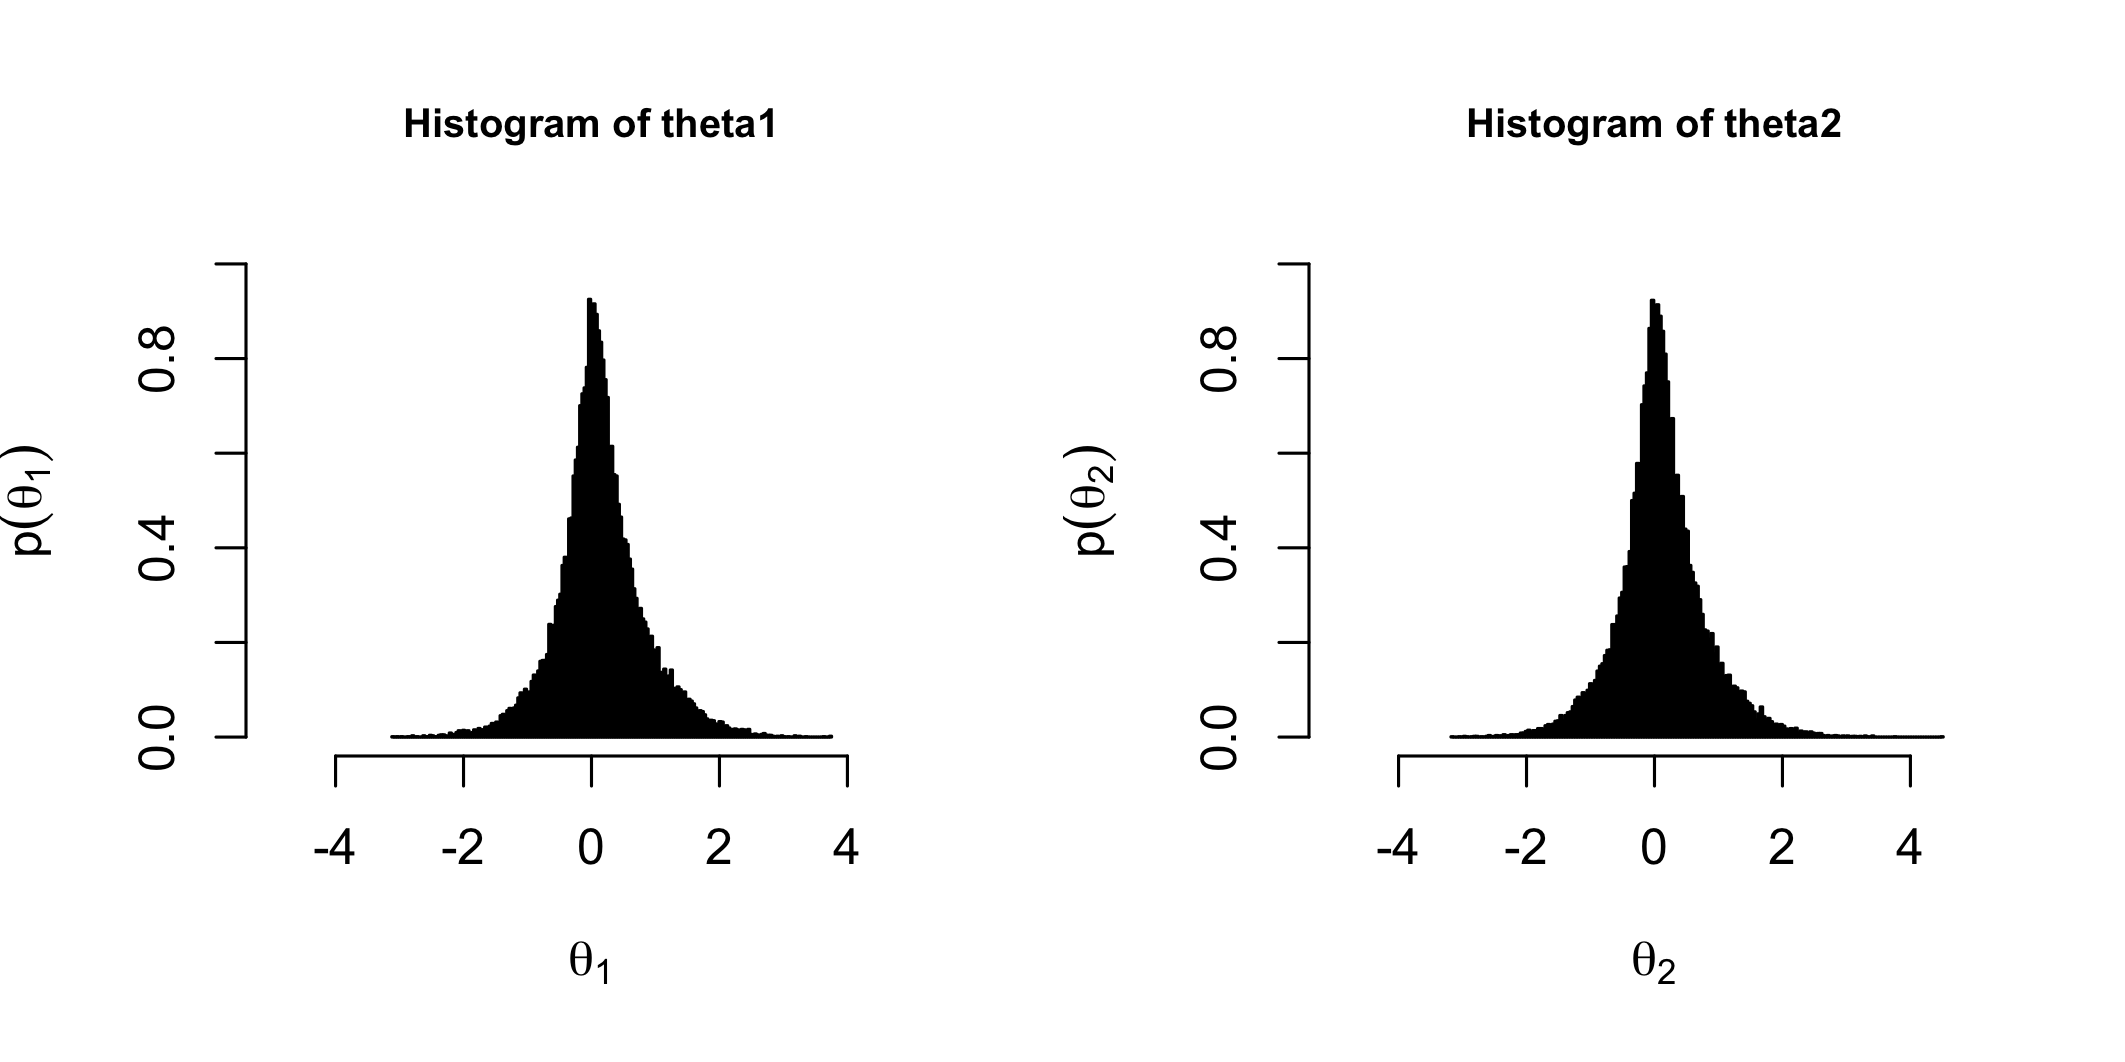
\includegraphics[width=0.6\linewidth]{pictures/fig02-gs-histogram.png}
    \caption{Sampling Histograms for $\theta_1$ and $\theta_2$ }
    \label{fig:gs-histogram}
\end{figure}

\begin{figure}[h!]
    \centering
    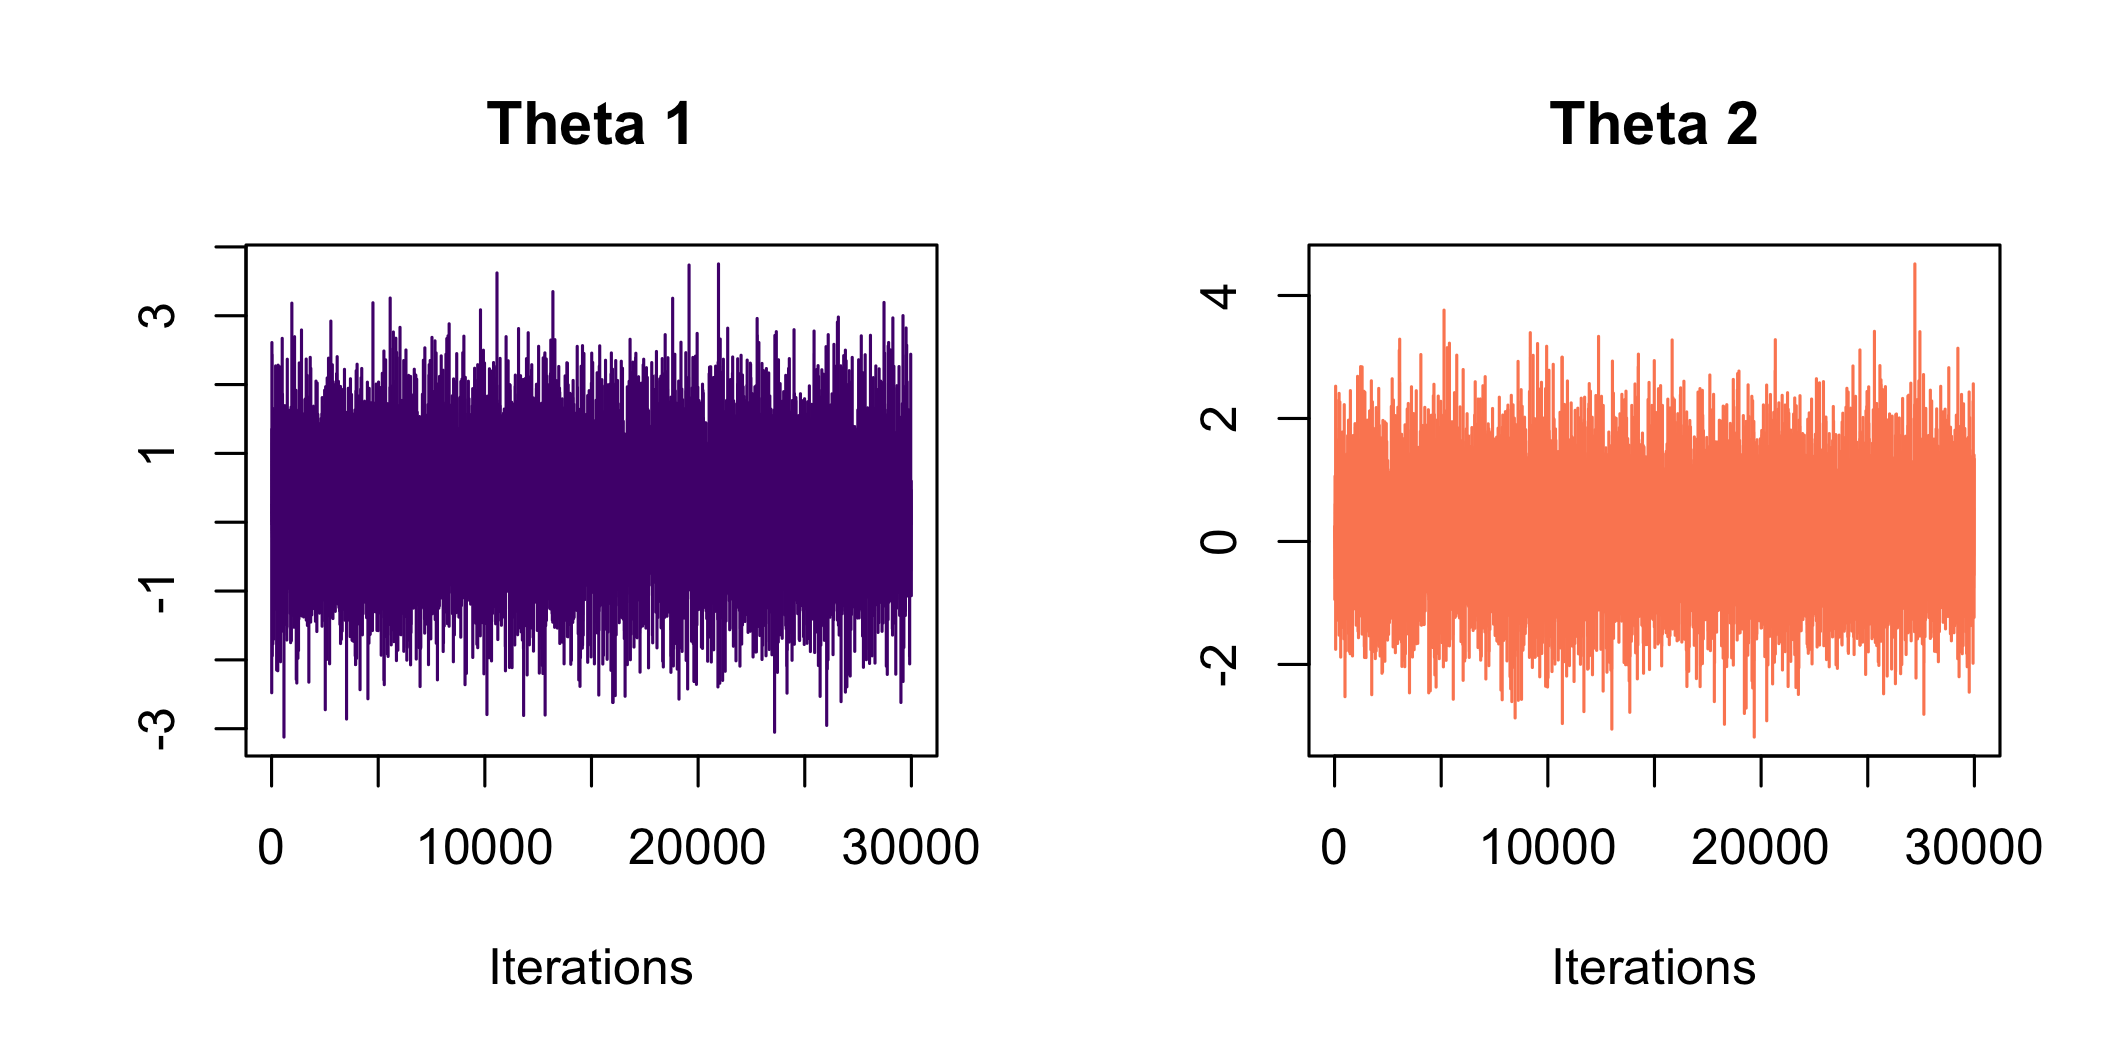
\includegraphics[width=0.6\linewidth]{pictures/fig01-gs-traceplot.png}
    \caption{Trace plots of $\theta_1$ and $\theta_2$ chains }
    \label{fig:gs-traceplot}
\end{figure}



\begin{table}[h!]
\centering
\caption{Summary statistics for Gibbs Sampler Chains.}
\begin{tabular}{lcccc}
\toprule
\textbf{} & \textbf{Mean} & \textbf{Median} & \textbf{95\% HPD Interval}  & \textbf{95\% Equal Tail} \\
\midrule
$\theta_1$ & 0.13877 & 0.09255 & [-1.192072, 1.657779] & [-1.208464, 1.643236] \\
$\theta_2$ & 0.10127 & 0.06755 & [-1.283651, 1.535148] & [-1.208464, 1.643236] \\
\bottomrule
\end{tabular}
\label{tab:summary_gs}
\end{table}

The acceptance rate of Gibbs sampling technique, based on full conditional distributions, is always 1(100\%). This is because every new value is sampled from the target distribution conditioned on valid values of all other variables $i.e$ the proposal distribution is the same as the full conditional distribution.
\subsection{Use the Geweke convergence diagnostic test on the generated chains and interpret your results.}
\textbf{Solution}

The Geweke test, is a formal convergence diagnostic test that assesses stationarity by comparing the means of the early (10\%) and late (50\%) portions of a Markov chain. From Table \ref{tab:geweke_gs} summaries, all $Z-score$ were within the acceptance region suggesting no evidence that the parameter mean of the late part is different from the early part. Figure \ref{fig:gs-geweke}   affirms the findings of the Geweke diagnostic test as the points fall within the acceptance window. We can there conclude that the chains likely achieved good convergence.
\begin{table}[h!]
\centering
\caption{Geweke convergence diagnostic test result}
\begin{tabular}{lcccc}
\toprule
\textbf{} & \textbf{1st window(\%)} & \textbf{2nd window(\%)} & \textbf{$Z-score$} & \textbf{Acceptance Interval($\alpha = 0.05$)}  \\
\midrule
$\theta_1$ & 0.1& 0.5 & -0.1207  & [-1.96, 1.96] \\
$\theta_2$ & 0.1& 0.5 & -0.8128 & [-1.96, 1.96] \\
\bottomrule
\end{tabular}
\label{tab:geweke_gs}
\end{table}

\begin{figure}[h!]
    \centering
    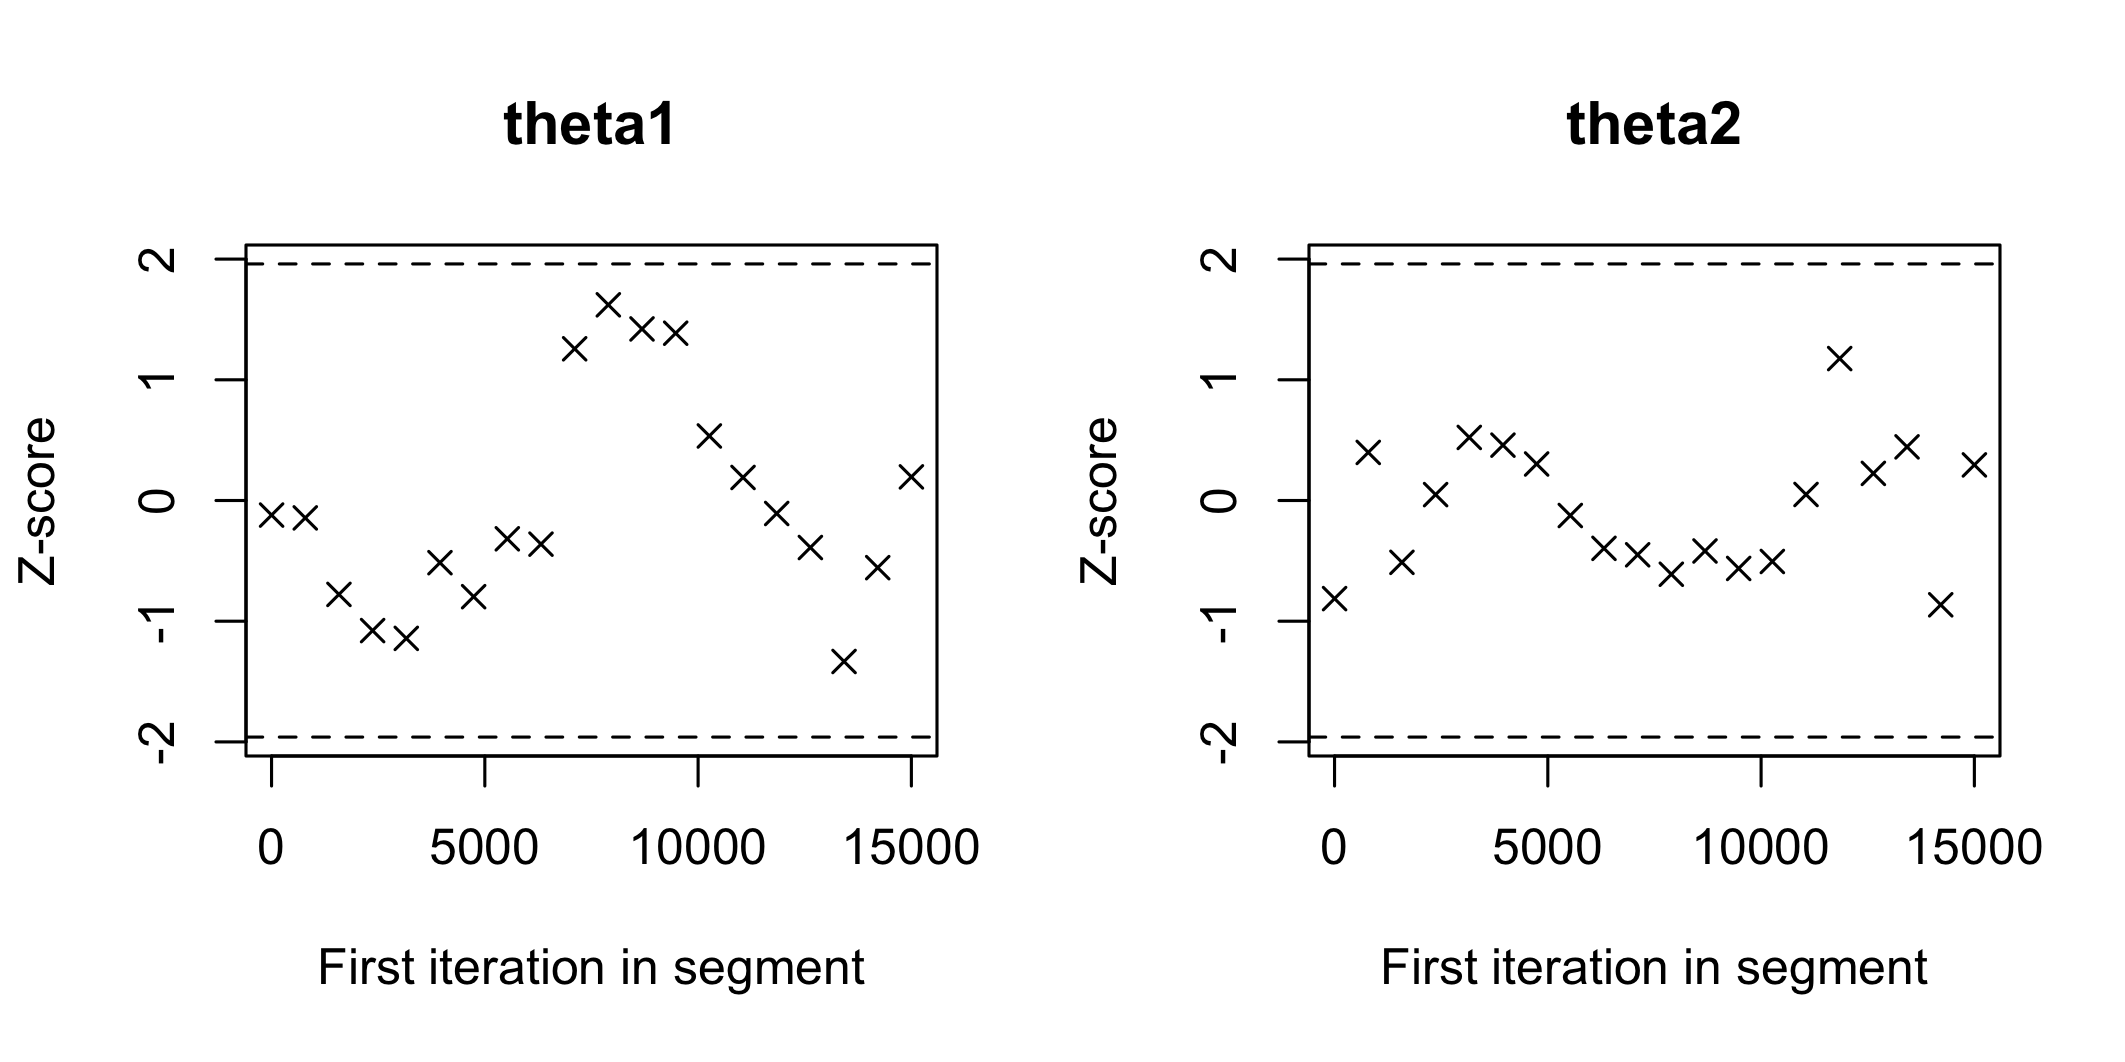
\includegraphics[width=0.6\linewidth]{pictures/fig05-gs-geweke.png}
    \caption{Geweke diagnostics plots for  $\theta_1$ and $\theta_2$ }
    \label{fig:gs-geweke}
\end{figure}


\subsection{Compute a point estimate for $\theta_1$ and a 95\% quantile-based credible interval}
\textbf{Solution}

Given the symmetric nature of $\theta_1$ values, either the mean and median could be sufficiently be used as a point estimate for $\theta_1$. As we can see from table \ref{tab:summary_gs}, the mean and the median of $\theta_1$ is 0.13877 and 0.09255 respectively. The 95\% equal tail is [-1.208464,1.643236].


\subsection{Using your generated chains, estimate the probability $P(\theta_1 > 0.5)$.}
\textbf{Solution}

The $p$ Monte Carlo value for which $p(\theta_1 > 0.5)$ was calculated as  $\frac{1 + \sum (\theta_1 > 0.5)}{30000 + 1}$ and found to be 0.2388587; $p(\theta_1 > 0.5)$ is thus 23.9 \%.


\section{Part 2 - The Metropolis algorithm}
\subsection{Write the log posterior distribution \( \log p(\theta|D) \) and obtain analytically the gradient
\[\nabla_\theta \log p(\theta|D) = \left( \frac{\partial \log p(\theta|D)}{\partial \theta_1}, \frac{\partial \log p(\theta|D)}{\partial \theta_2} \right)^\top \]
and Hessian matrix:
\[\nabla^2_\theta \log p(\theta|D) = 
\begin{pmatrix}
\frac{\partial^2 \log p(\theta|D)}{\partial \theta_1^2} & \frac{\partial^2 \log p(\theta|D)}{\partial \theta_1 \partial \theta_2} \\
\frac{\partial^2 \log p(\theta|D)}{\partial \theta_2 \partial \theta_1} & \frac{\partial^2 \log p(\theta|D)}{\partial \theta_2^2} 
\end{pmatrix}.\]}
\textbf{Solution}\\
The log posterior distribution could be written as:
\[
\log(p(\theta|D)) \propto -8\theta_1^2\theta_2^2 - 0.5\theta_1^2 - 0.5\theta_2^2 + \cos(2\pi + 0.3)\theta_1\theta_2 + 0.3\theta_1 + 0.2\theta_2
\]
By taking the first and second-order partial derivatives with regard to \(\theta_1\) and \(\theta_2\), of \(\log p(\theta|D)\),
we obtain the gradient as follows:
\[
\nabla_\theta \log p(\theta|D) = \left( -16\theta_1\theta_2^2 - \theta_1 + \cos(2\pi + 0.3)\theta_2 + 0.3, -16\theta_1^2\theta_2 - \theta_2 + \cos(2\pi + 0.3)\theta_1 + 0.2 \right)^\top
\]
And the Hessian matrix is as follows:
\[
\nabla^2_\theta \log p(\theta|D) = 
\begin{pmatrix}
-16\theta_2^2 - 1 & -32\theta_1\theta_2 + \cos(2\pi + 0.3) \\
-32\theta_1\theta_2 + \cos(2\pi + 0.3) & -16\theta_1^2 - 1
\end{pmatrix}
\]

\subsection{Using the gradient and Hessian matrix obtained in the previous step, implement a Newton-Raphson algorithm in R to find the posterior mode of \( p(\theta|D) \) and denote by
\[
\theta^*_{NR} = (\theta^*_1, \theta^*_2)^\top
\]
the mode after convergence of the algorithm. (Note: round \( \theta^*_{NR} \) to five digits after the decimal point).}
\textbf{Solution}\\
The Pseudo-code of Newton-Raphson algorithm to find the mode of \( p(\theta|D) \) is as follows:

\begin{algorithm}
\begin{algorithmic}[1]
\State Set tolerance \( \epsilon \), arbitrary initial distance \( d \), initialize \( \theta^{(0)} \) and set \( m = 0 \).
\While{$d > \epsilon$}
    \State \( \theta^{(m+1)} = \theta^{(m)} - \left( \nabla^2 \log p(\theta^{(m)}|D) \right)^{-1} \nabla \log p(\theta^{(m)}|D) \)
    \State Compute distance \( d = \|\theta^{(m+1)} - \theta^{(m)}\| \).
\EndWhile
\State At convergence, return \( \theta^M \).
\end{algorithmic}
\end{algorithm}

The following R code was implemented to obtain the posterior mode:

\lstset{
    language=R,
    basicstyle=\ttfamily\small,
    breaklines=true,
    breakatwhitespace=true,
    columns=fullflexible,
    backgroundcolor=\color{white},
    keywordstyle=\color{black},
    commentstyle=\color{black},
    stringstyle=\color{black},
    showstringspaces=false,
    numbers=left,
    numberstyle=\tiny\color{black}
}

\begin{lstlisting}
# define constants
A <- 16
B <- cos(2 * pi + 0.3)
C1 <- 0.3
C2 <- 0.2

# Define the gradient function in the global environment
gradient_theta <- function(theta = c(1, 2)) {
  t1 <- theta[1]
  t2 <- theta[2]
  grad1 <- -A * t1 * t2^2 - t1 + B * t2 + C1
  grad2 <- -A * t1^2 * t2 - t2 + B * t1 + C2
  return(c(grad1, grad2))
}

# Define the Hessian function in the global environment
hessian_theta <- function(theta = c(1, 2)) {
  t1 <- theta[1]
  t2 <- theta[2]
  h11 <- -A * t2^2 - 1
  h12 <- h21 <- -2 * A * t1 * t2 + B
  h22 <- -A * t1^2 - 1
  return(matrix(c(h11, h12, h21, h22), nrow = 2))
}

NewtonRaphson <- function(theta0 = c(1, 2), tolerance = 1e-10, iteration = 1000) {
  for (i in 1:iteration) {
    grad_theta0 <- gradient_theta(theta0)
    hes_theta0 <- hessian_theta(theta0)
    theta1 <- theta0 - solve(hes_theta0, grad_theta0) # Calculate next value of theta
    distance <- sum(abs(theta1 - theta0))
    if (distance < tolerance) { # Once distance between theta1 and theta0 gets sufficiently small, output result
      result <- round(theta1, 5)
      return(list("mode theta" = result, paste("Converged at iteration", i)))
    }
    # If convergence not reached, set theta1 as theta0 and continue
    theta0 <- theta1
  }
  print('Newton-Raphson algorithm did not converge. Choose a larger number of iterations.')
}

theta_NR_star <- NewtonRaphson()$'mode theta'
theta_NR_star

\end{lstlisting}
Using the above algorithm, the posterior mode of \( p(\theta|D) \) was found to locate at
\[ \theta^*_{NR} = (0.2997; 0.1996)^\top \]

\subsection{Compute a Laplace approximation to \( p(\theta|D) \) around \( \theta^*_{NR} \). Report the covariance matrix \( \Sigma^* \) of the Laplace approximation. (Note: round your results to five digits after the decimal point).}
\textbf{Solution}\\
Using Laplace approximation around \( \theta^*_{NR} \), the posterior distribution \( p(\theta|D) \) is approximated
by a Gaussian distribution with
\begin{itemize}
    \item Mean \( \mu^{0} = \theta^*_{NR} - (\nabla^2 \log p(\theta^*_{NR}|D))^{-1} \nabla \log p(\theta^*_{NR}|D) \)
    \item Covariance matrix \( \Sigma^* = (\nabla^2 \log p(\theta^*_{NR}|D))^{-1} \)
\end{itemize}
With \( \nabla \log p(\theta^*_{NR}|D) \) and \( \nabla^2 \log p(\theta^*_{NR}|D))^{-1} \) the gradient and Hessian, respectively, of the
log target posterior distribution, evaluated at \( \theta^*_{NR} \).

Using the calculation from Question 1, the covariance matrix \( \Sigma^* \) is:
\[ \Sigma^* =
\begin{pmatrix}
0.7935 & -0.3121 \\
-0.3121 & 0.5330
\end{pmatrix}
\]

And the mean \( \mu^{0} \):
\[ \mu^{0} =
\begin{pmatrix}
0.2997 \\
0.1996
\end{pmatrix}
\]

Thus the distribution of the approximated posterior distribution is:
\[ \tilde{p}_G(\theta|D) \sim N\left(
\begin{pmatrix}
0.2997 \\
0.1996
\end{pmatrix}
,
\begin{pmatrix}
0.7935 & -0.3121 \\
-0.3121 & 0.5330
\end{pmatrix}
\right) \]

\subsection{In R, write a random-walk Metropolis algorithm to explore the joint posterior \( p(\theta|D) \) using a Gaussian proposal with covariance matrix \( \tilde{\Sigma} = c\Sigma^* \). Use a chain of length \( M = 50,000 \) and tune \( c \) to (approximately) reach the optimal acceptance rate of 23\%. Please specify \textit{set.seed(1993)} for the sake of reproducibility of your results.}
\textbf{Solution}\\
The pseudo-code of the random-walk Metropolis algorithm is as follows:
\begin{enumerate}
    \item Choose initial value \( \theta^{0} \) satisfying \( p(\theta^{0}|D) > 0 \)
    \item For \( m \) in 1 to \( M \) do:
    \begin{enumerate}
        \item Sample \( \tilde{\theta}^{(m)} \sim q(\cdot|\theta^{(m-1)}) \)
        \item Compute the log ratio \( \log \varrho(\theta^{(m-1)}, \tilde{\theta}^{(m)}) = \log \frac{p(\tilde{\theta}^{(m)}|D)}{p(\theta^{(m-1)}|D)} \)
        \item Sample \( u \sim U(0, 1) \)
        \item If $\log(\varrho) \geq 0 \; \| \; u \leq \exp(\log(\varrho))$, set $\theta^{(m)} \gets \tilde{\theta}^{(m)}$ (accept candidate)
        \item Else \( \theta^{(m)} \leftarrow \theta^{(m-1)} \) (reject candidate)
    \end{enumerate}
    \item End for.
\end{enumerate}

The following Metropolis algorithm was implemented in R to explore \( p(\theta|D) \):

\begin{lstlisting}
Metropolis <- function(M = 51000, burn_in = 1000, seed = 1993, 
                       theta_start = c(0.29970, 0.19955), c_tune = 2 )
{
  set.seed(seed)
  
  # Joint log posterior distribution
  log_posterior <- function(theta)
  {
    t1 <- theta[1]
    t2 <- theta[2]
    return(-1/2*(A*t1^2*t2^2 + t1^2 + t2^2 - 2*B*t1*t2 - 2*C1*t1 - 2*C2*t2))
  }
  
  # Starting value for theta 1 and theta 2
  theta <- array(dim = c(2, M))
  theta[, 1] <- theta_start
  n_accept <- 0
  
  # Gaussian proposal
  # Covariance matrix
  theta_NR_star <- NewtonRaphson()$'mode theta' #The NewtonRaphson function built in Q2
  sigma_star <- round(solve(-hessian_theta(theta = theta_NR_star)),5)
  sigma_tilde <- c_tune*sigma_star
  
  # Metropolis loop
  for (i in 2:M)
  {
    # New proposed theta
    theta_prop <- theta[,i - 1] + rmvnorm(n = 1, 
                                        mean = c(0,0), sigma = sigma_tilde)
    # Log ratio for accept-reject decision
    logr <- log_posterior(theta_prop) - log_posterior(theta[,i - 1])
    
    # Accept or reject
    u <- runif(1)
    if (logr >= 0 || u <= exp(logr))
    { #Accept
      theta[,i] <- theta_prop
      n_accept <- n_accept + 1
    } 
    else 
    { #Reject, stay where theta is
      theta[,i] <- theta[, i - 1]
    }
  }
  # Exclude burn-in
  theta <- theta[,-c(1:burn_in)]
  # Output
  accept_rate <- round(n_accept/(M - 1), digits = 3) * 100
  rownames(theta) <- c("Theta1","Theta2")
  output <- list(theta = theta,
                 M = M, 
                 burn_in = burn_in,
                 log_posterior = log_posterior)
  print(paste("Acceptance rate:", accept_rate,"%"))
  return(invisible(output))
}

MCMC_run <- Metropolis(c_tune = 2.8)

\end{lstlisting}

Our MCMC chain had 51000 iterations; the first 10000 were burn-in period. The
starting point of \( \theta \) was set at \( \theta^*_{NR} \). The tuning factor \( c \) was set at 2.8 to give the acceptance
rate of 23.3\%. The trace plots, Q-Q plots, running mean plots, and Geweke diagnostic (Figure
\ref{fig:mh-traceplot}, \ref{fig:mh-qqplot}, \ref{fig:mh-runmean}, and \ref{fig:mh-geweke}) showed good signs of convergence.

\begin{figure}[H]
    \centering    \includegraphics[width=0.8\textwidth]{pictures/fig01-mh-traceplot.png}
    \caption{Trace plots of \( \theta_1 \) and \( \theta_2 \)}
    \label{fig:mh-traceplot}
\end{figure}

\begin{figure}[H]
    \centering    \includegraphics[width=0.8\textwidth]{pictures/fig03-mh-qqplots.png}
    \caption{Q-Q plots of \( \theta_1 \) and \( \theta_2 \)}
    \label{fig:mh-qqplot}
\end{figure}

\begin{figure}[H]
    \centering    \includegraphics[width=0.8\textwidth]{pictures/fig04-mh-runmean.png}
    \caption{Running mean plots of \( \theta_1 \) and \( \theta_2 \)}
    \label{fig:mh-runmean}
\end{figure}

\begin{figure}[H]
    \centering    \includegraphics[width=0.8\textwidth]{pictures/fig05-mh-geweke.png}
    \caption{Time series plots of Geweke test statistic for \( \theta_1 \) and \( \theta_2 \)}
    \label{fig:mh-geweke}
\end{figure}

The summary statistics of posterior $\theta_1$ and $\theta_2$ is given in Table \ref{tbl:mh-summary}.

\begin{table}[H]
\centering
\begin{tabular}{lcccccc}
\hline
Parameter & Posterior mean & Posterior median & Posterior SD & 95\% equal tail CI & 95\% HPD interval \\
\hline
$\theta_1$ & 0.165 & 0.084 & 0.686 & -1.101 ; 1.726 & -1.101 ; 1.723 \\
$\theta_2$ & 0.101 & 0.066 & 0.648 & -1.210 ; 1.579 & -1.231 ; 1.548 \\
\hline
\end{tabular}
\caption{Summary measures of the posterior distribution of $\theta_1$ and $\theta_2$}
\label{tbl:mh-summary}
\end{table}

\subsection{Using your generated chains, estimate the probability \( P\left(\frac{\theta_1}{\theta_2} > 0.45\right) \).}
\textbf{Solution}\\
The probability \( P\left(\frac{\theta_1}{\theta_2} > 0.45\right) \) was calculated as the proportion of the MCMC chain that produced the ratio \( \frac{\theta_1}{\theta_2} > 0.45 \). It was estimated to be 0.374.

\printbibliography

\section{Appendix}

\begin{figure}[!h]
    \centering
    \includegraphics[width=1\linewidth]{pictures/caterpillar.png}
    \caption{Caterpillar plot}
    \label{fig:fullcaterpillar}
\end{figure}

\begin{table}[h!]
\centering
\tiny
\caption{Posterior participation rates for each municipality.}
\label{tab:params1}
\begin{tabular}{|llllll|llllll|}
\hline
\textbf{Node} & \textbf{Mean} & \textbf{SD} & \textbf{MC error} & \textbf{2.5\%} &  \textbf{97.5\%} & \textbf{Node} & \textbf{Mean} & \textbf{SD} & \textbf{MC error} & \textbf{2.5\%} &  \textbf{97.5\%} \\ \hline
pi[1]  & 0.4275  & 0.005038  & 3.657e-05 & 0.4177 &0.4375 & pi[108] & 0.3734 & 0.013496 & 9.759e-05 & 0.3472 &0.3998  \\ 
pi[2]  & 0.5428  & 0.008585  & 6.460e-05 & 0.5258 &0.5593 & pi[109] & 0.5438 & 0.014461  & 1.082e-04 & 0.5153 &0.5719 \\ 
pi[3]  & 0.4894  & 0.008549  & 6.226e-05 & 0.4727 &0.5064 & pi[110] & 0.5384 & 0.014211 & 1.035e-04 & 0.5109 &0.5664 \\ 
pi[4]  & 0.4996  & 0.013029  & 9.616e-05 & 0.4740 &0.5255 & pi[111] & 0.5128 & 0.014842  & 1.083e-04 & 0.4838 &0.5422 \\ 
pi[5]  & 0.4409  & 0.012736  & 9.319e-05 & 0.4161 &0.4661 & pi[112] & 0.5487 & 0.010479   & 7.641e-05 & 0.5280 &0.5691 \\ 
pi[6]  & 0.5660  & 0.013331  & 9.763e-05 & 0.5400 &0.5919 & pi[113] & 0.4838 & 0.031350   & 2.282e-04 & 0.4228 &0.5456 \\
pi[7]  & 0.4189  & 0.022645  & 1.632e-04 & 0.3747 &0.4634 & pi[114] & 0.5085 & 0.008513   & 6.211e-05 & 0.4920 &0.5254\\ 
pi[8]  & 0.3773  & 0.002169  & 1.569e-05 & 0.3731 &0.3815 & pi[115] & 0.4789 & 0.015222   & 1.142e-04 & 0.4493 &0.5088 \\
pi[9]  & 0.4881  & 0.012167  & 8.996e-05 & 0.4643 &0.5117 & pi[116] & 0.5782 & 0.016680  & 1.244e-04 & 0.5457 &0.6108 \\
pi[10] & 0.5051  & 0.015735  & 1.153e-04 & 0.4740 &0.5360 & pi[117] & 0.4664 & 0.014424   & 1.049e-04 & 0.4383 &0.4951 \\ 
pi[11] & 0.5570  & 0.012566  & 9.197e-05 & 0.5323 &0.5817 & pi[118] & 0.5120 & 0.014060   & 1.029e-04 & 0.4848 &0.5396 \\ 
pi[12] & 0.5383  & 0.016358  & 1.221e-04 & 0.5059 &0.5702 & pi[119] & 0.4951 & 0.012417   & 9.180e-05 & 0.4709 &0.5193 \\ 
pi[13] & 0.3753  & 0.008073  & 6.014e-05 & 0.3596 &0.3909 & pi[120] & 0.5245 & 0.007843   & 5.620e-05 & 0.5092 &0.5398 \\ 
pi[14] & 0.5194  & 0.012144  & 8.947e-05 & 0.4957 &0.5432 & pi[121] & 0.4992 & 0.015035   & 1.093e-04 & 0.4696 &0.5286 \\ 
pi[15] & 0.4442  & 0.014480  & 1.050e-04 & 0.4158 &0.4725 & pi[122] & 0.4826 & 0.009452  & 6.780e-05 & 0.4642 &0.5012 \\ 
pi[16] & 0.5275  & 0.027320  & 2.031e-04 & 0.4739 &0.5806 & pi[123] & 0.5599 & 0.011763   & 8.548e-05 & 0.5367 &0.5827 \\ 
pi[17] & 0.5454  & 0.009926  & 7.382e-05 & 0.5258 &0.5647 & pi[124] & 0.5764 & 0.010742   & 7.999e-05 & 0.5553 &0.5974 \\ 
pi[18] & 0.5427  & 0.011259  & 8.312e-05 & 0.5207 &0.5647 & pi[125] & 0.5061 & 0.013514  & 9.922e-05 & 0.4795 & 0.5327\\ 
pi[19] & 0.5447  & 0.011227  & 8.385e-05 & 0.5224 &0.5666 &pi[126] & 0.4774 & 0.015454  & 1.131e-04 & 0.4472 &0.5077 \\ 
pi[20] & 0.3363  & 0.009023  & 6.542e-05 & 0.3186 &0.3539 & pi[127] & 0.5378 & 0.008646  & 6.266e-05 & 0.5207 &0.5548 \\ 
pi[21] & 0.4957 & 0.013998   & 1.046e-04 & 0.4683 &0.5233 & pi[128] & 0.5450 & 0.017873  & 1.319e-04 & 0.5100 &0.5802 \\
pi[22] & 0.5130 & 0.017600   & 1.261e-04 & 0.4784 &0.5471 & pi[129] & 0.6004 & 0.010471  & 7.577e-05 & 0.5798 &0.6208 \\
pi[23] & 0.5272 & 0.007048   & 5.143e-05 & 0.5133 &0.5409 & pi[130] & 0.5168 & 0.012392  & 9.084e-05 & 0.4928 &0.5413 \\
pi[24] & 0.5312 & 0.013181   & 9.720e-05 & 0.5051 &0.5571 & pi[131] & 0.5964 & 0.011982   & 8.722e-05 & 0.5729 &0.6199 \\
pi[25] & 0.5281 & 0.011805   & 8.872e-05 & 0.5049 &0.5511 & pi[132] & 0.4172 & 0.019145  & 1.411e-04 & 0.3797 &0.4552 \\
pi[26] & 0.5296 & 0.014922   & 1.100e-04 & 0.5003 &0.5589 & pi[133] & 0.4926 & 0.007368   & 5.639e-05 & 0.4781 &0.5069 \\
pi[27] & 0.4055 & 0.030487   & 2.299e-04 & 0.3468 &0.4656 & pi[134] & 0.4655 & 0.015907  & 1.175e-04 & 0.4344 &0.4968 \\
pi[28] & 0.5304 & 0.006638   & 4.883e-05 & 0.5175 &0.5435 & pi[135] & 0.4814 & 0.009087  & 6.686e-05 & 0.463 & 0.4993 \\
pi[29] & 0.5762 & 0.014509   & 1.054e-04 & 0.5474 &0.6047 & pi[136] & 0.5375 & 0.010164  & 7.336e-05 & 0.5175 &0.5572 \\
pi[30] & 0.5347 & 0.007965   & 5.834e-05 & 0.5189 &0.5502 & pi[137] & 0.4799 & 0.013953  & 1.037e-04 & 0.4525 &0.5072 \\
pi[31] & 0.4503 & 0.009194   & 6.825e-05 & 0.4324 &0.4683 & pi[138] & 0.5119 & 0.016027   & 1.200e-04 & 0.4803 &0.5432 \\
pi[32] & 0.6280 & 0.012256   & 8.999e-05 & 0.6040 &0.6520 & pi[139] & 0.4271 & 0.010479   & 7.826e-05 &0.4067 &0.4475 \\
pi[33] & 0.5349 & 0.012932   & 9.496e-05 & 0.5094 &0.5600 & pi[140] & 0.5698 & 0.015686   & 1.152e-04 & 0.5393 &0.6004 \\
pi[34] & 0.5393 & 0.011938   & 8.545e-05 & 0.5159 &0.5625 & pi[141] & 0.4544 & 0.005654   & 4.158e-05 & 0.4434 &0.4656 \\
pi[35] & 0.3761 & 0.011909   & 8.590e-05 & 0.3529 &0.3997 & pi[142] & 0.2396 & 0.010652  & 7.846e-05 & 0.2191 &0.2610 \\
pi[36] & 0.5007 & 0.013298   & 9.640e-05 & 0.4750 &0.5270 & pi[143] & 0.5457 & 0.011909  & 8.693e-05 & 0.5223 &0.5693 \\
pi[37] & 0.4738 & 0.013370   & 9.583e-05 & 0.4476 &0.5000 & pi[144] & 0.5069 & 0.012224  & 9.112e-05 & 0.4830 &0.5308 \\
pi[38] & 0.5199 & 0.009898   & 7.012e-05 & 0.5005 &0.5393 & pi[145] & 0.4962 & 0.013382  & 1.002e-04 & 0.4698 &0.5222 \\
pi[39] & 0.4601 & 0.015044   & 1.098e-04 & 0.4311 &0.4902 & pi[146] & 0.5472 & 0.011322  & 8.254e-05 & 0.5251 &0.5694 \\
pi[40] & 0.5044 & 0.016431   & 1.212e-04 & 0.4721 &0.5367 & pi[147] & 0.5313 & 0.012997  & 9.554e-05 & 0.5057 &0.5565 \\
pi[41] & 0.4669 & 0.012342   & 9.069e-05 & 0.4430 &0.4913 & pi[148] & 0.5418 & 0.008471 & 6.213e-05 & 0.5252 &0.5585 \\
pi[42] & 0.5424 & 0.007536   & 5.593e-05 & 0.5275 &0.5570 & pi[149] & 0.4506 & 0.011788  & 8.661e-05 & 0.4275 &0.4738 \\
pi[43] & 0.5547 & 0.008304   & 5.975e-05 & 0.5384 &0.5711 & pi[150] & 0.5148 & 0.017184  & 1.245e-04 & 0.4813 &0.5490 \\
pi[44] & 0.5261 & 0.010334   & 7.669e-05 & 0.5061 &0.5464 & pi[151] & 0.4905 & 0.010589  & 7.716e-05 & 0.4697 &0.5113 \\
pi[45] & 0.5497 & 0.011446   & 8.534e-05 & 0.5272 &0.5721 & pi[152] & 0.4743 & 0.010709  & 7.911e-05 & 0.4533 &0.4953 \\
pi[46] & 0.5107 & 0.004253   & 3.096e-05 & 0.5024 &0.5189 & pi[153] & 0.5048 & 0.015842  & 1.150e-04 & 0.4740 &0.5361 \\
pi[47] & 0.5071 & 0.012264   & 8.794e-05 & 0.4830 &0.5313 & pi[154] & 0.4588 & 0.021292 & 1.564e-04 & 0.4177 &0.5009 \\
pi[48] & 0.5288 & 0.013529   & 9.833e-05 & 0.5023 &0.5551 & pi[155] & 0.4563 & 0.014811  & 1.087e-04 & 0.4277 &0.4855 \\
pi[49] & 0.4936 & 0.011399   & 8.288e-05 & 0.4713 &0.5159 & pi[156] & 0.4788 & 0.011880  & 8.541e-05 & 0.4556 &0.5021 \\
pi[50] & 0.3804 & 0.012539   & 9.389e-05 & 0.3557 &0.4050 & pi[157] & 0.4823 & 0.005239  & 3.823e-05 & 0.4721 &0.4927 \\
pi[51] & 0.5930 & 0.013727   & 9.897e-05 & 0.5660 &0.6195 & pi[158] & 0.5366 & 0.016559 & 1.254e-04 & 0.5041 &0.5690 \\
pi[52] & 0.5071 & 0.014029   & 1.018e-04 & 0.4795 &0.5345 & pi[159] & 0.4073 & 0.012388  & 9.328e-05 & 0.3832 &0.4315 \\
pi[53] & 0.5378 & 0.007278   & 5.266e-05 & 0.5233 &0.5519 & pi[160] & 0.4682 & 0.007733   & 5.644e-05 & 0.4531 &0.4835 \\
pi[54] & 0.4421 & 0.010306   & 7.600e-05 & 0.4218 &0.4622 & pi[161] & 0.4834 & 0.017711   & 1.314e-04 & 0.4488 &0.5179 \\
pi[55] & 0.4829 & 0.006945   & 4.994e-05 & 0.4691 &0.4964 & pi[162] & 0.5597 & 0.008984   & 6.609e-05 & 0.5417 &0.5772 \\
pi[56] & 0.5129 & 0.016317   & 1.182e-04 & 0.4813 &0.5448 & pi[163] & 0.5824 & 0.011227   & 8.306e-05 & 0.5605 &0.6044 \\
pi[57] & 0.5887 & 0.014662   & 1.069e-04 & 0.5599 &0.6172 & pi[164] & 0.2471 & 0.019144   & 1.400e-04 & 0.2108 &0.2860 \\
pi[58] & 0.5459 & 0.010921   & 8.004e-05 & 0.5244 &0.5672 & pi[165] & 0.5334 & 0.015647   & 1.154e-04 & 0.5026 &0.5640 \\
pi[59] & 0.5310 & 0.010569   & 7.701e-05 & 0.5102 &0.5518 & pi[166] & 0.4860 & 0.016626   & 1.224e-04 & 0.4532 &0.5186 \\
pi[60] & 0.4860 & 0.009543   & 6.957e-05 & 0.4673 &0.5047 & pi[167] & 0.5174 & 0.027476   & 2.000e-04 & 0.4641 &0.5706 \\
pi[61] & 0.5021 & 0.011825   & 8.745e-05 & 0.4788 &0.5254 & pi[168] & 0.5732 & 0.009661   & 6.998e-05 & 0.5541 &0.5920 \\
pi[62] & 0.3330 & 0.006976   & 5.142e-05 & 0.3194 &0.3466 & pi[169] & 0.5201 & 0.007488   & 5.551e-05 & 0.5054 &0.5347 \\
pi[63] & 0.5326 & 0.010012   & 7.472e-05 & 0.5130 &0.5521 &pi[170] & 0.5804 & 0.007488  & 5.536e-05 & 0.5656 &0.5950 \\
pi[64] & 0.1564 & 0.015028   & 1.096e-04 & 0.1280 &0.1869 &pi[171] & 0.4747 & 0.010988  & 7.967e-05 & 0.4530 &0.4963 \\
pi[65] & 0.4987 & 0.011338   & 8.302e-05 & 0.4766 &0.5211 &pi[172] & 0.5750 & 0.011846  & 8.526e-05 & 0.5519 &0.5978\\
pi[66] & 0.5062 & 0.010450   & 7.540e-05 & 0.4857 &0.5267 &pi[173] & 0.5785 & 0.011837  & 8.611e-05 & 0.5554 &0.6019 \\
pi[67] & 0.4854 & 0.010018   & 7.529e-05 & 0.4655 &0.5048 &pi[174] & 0.5153 & 0.018770  & 1.403e-04 & 0.4791 &0.5524 \\
pi[68] & 0.5067 & 0.010238   & 7.456e-05 & 0.4866 &0.5270 &pi[175] & 0.5653 & 0.008955  & 6.608e-05 & 0.5476 &0.5828 \\
pi[69] & 0.5700 & 0.010156   & 7.413e-05 & 0.5502 &0.5898 &pi[176] & 0.4865 & 0.007503  & 5.466e-05 & 0.4718 &0.5013 \\
pi[70] & 0.5280 & 0.007866   & 5.760e-05 & 0.5125 &0.5434 &pi[177] & 0.3055 & 0.011370  & 8.310e-05 & 0.2836 &0.3277 \\
pi[71] & 0.4572 & 0.015740   & 1.145e-04 & 0.4265 &0.4880 &pi[178] & 0.5414 & 0.009289 & 6.678e-05 & 0.5234 &0.5593 \\
pi[72] & 0.5443 & 0.012916   & 9.492e-05 & 0.5191 &0.5696 &pi[179] & 0.5669 & 0.011598  & 8.458e-05 & 0.5442 &0.5895 \\
pi[73] & 0.5186 & 0.007362   & 5.445e-05 & 0.5044 &0.5331 &pi[180] & 0.4454 & 0.005429  & 4.040e-05 & 0.4346 &0.4560 \\
pi[74] & 0.4688 & 0.018505   & 1.338e-04 & 0.4327 &0.5050 &pi[181] & 0.5470 & 0.014923  & 1.108e-04 & 0.5176 &0.5765 \\
pi[75] & 0.4472 & 0.005708   & 4.196e-05 & 0.4360 &0.4584 &pi[182] & 0.4279 & 0.010582  & 7.807e-05 & 0.4073 &0.4489 \\
pi[76] & 0.4320 & 0.003233   & 2.435e-05 & 0.4257 &0.4383 &pi[183] & 0.5638 & 0.014357  & 1.064e-04 & 0.5354 &0.5917 \\
pi[77] & 0.4307 & 0.007833   & 5.844e-05 & 0.4154 &0.4460 &pi[184] & 0.4170 & 0.008219  & 5.895e-05 & 0.4009 &0.4329 \\
pi[78] & 0.4541 & 0.015977   & 1.168e-04 & 0.4228 &0.4856 &pi[185] & 0.4514 & 0.011407  & 8.180e-05 & 0.4289 &0.4738 \\
pi[79] & 0.5386 & 0.013234   & 9.167e-05 & 0.5127 &0.5648 &pi[186] & 0.5526 & 0.009564 & 6.925e-05 & 0.5337 &0.5711 \\
pi[80] & 0.4949 & 0.018693   & 1.396e-04 & 0.4585 &0.5310 &pi[187] & 0.5471 & 0.016246  & 1.172e-04 & 0.5151 &0.5790\\
pi[81]  & 0.4863 & 0.014706  & 1.108e-04 & 0.4575 &0.5152 &pi[188] & 0.2789 & 0.047969  & 3.546e-04 & 0.1890 &0.3769 \\
pi[82]  & 0.3659 & 0.007479  & 5.348e-05 & 0.3514 &0.3806 &pi[189] & 0.5133 & 0.014291  & 1.039e-04 & 0.4854 &0.5413 \\
pi[83]  & 0.5605 & 0.013386  & 9.747e-05 & 0.5342 &0.5865 &pi[190] & 0.4618 & 0.009336  & 6.966e-05 & 0.4435 &0.4801 \\
pi[84]  & 0.5291 & 0.011927  & 8.927e-05 & 0.5057 &0.5526 & pi[191] & 0.5763 & 0.018509  & 1.379e-04 & 0.5395 &0.6121 \\
pi[85]  & 0.4799 & 0.010670  & 7.665e-05 & 0.4592 &0.5008 &pi[192] & 0.5462 & 0.007762  & 5.622e-05 & 0.5311 &0.5614 \\
pi[86]  & 0.5199 & 0.015906  & 1.174e-04 & 0.4889 &0.5516 &pi[193] & 0.5100 & 0.014965  & 1.102e-04 & 0.4803 &0.5390 \\
pi[87]  & 0.3665 & 0.007468  & 5.312e-05 & 0.3518 &0.3810 &pi[194] & 0.5173 & 0.009717  & 7.122e-05 & 0.4981 &0.5362 \\
pi[88]  & 0.5399 & 0.014268  & 1.030e-04 & 0.5122 &0.5678 &pi[195] & 0.5303 & 0.013325  & 9.717e-05 & 0.5043 &0.5566 \\
pi[89]  & 0.4903 & 0.009554  & 6.875e-05 & 0.4719 &0.5089 &pi[196] & 0.4079 & 0.015859  & 1.165e-04 & 0.3767 &0.4387 \\
pi[90]  & 0.5961 & 0.012025  & 8.714e-05 & 0.5726 &0.6197 &pi[197] & 0.5612 & 0.017203  & 1.239e-04 & 0.5272 &0.5951 \\
pi[91]  & 0.5089 & 0.008848  & 6.342e-05 & 0.4914 &0.5261 &pi[198] & 0.4706 & 0.012567  & 9.073e-05 & 0.4461 &0.4952 \\
pi[92]  & 0.5187 & 0.005273  & 3.726e-05 & 0.5082 &0.5291 &pi[199] & 0.5544 & 0.009479  & 7.065e-05 & 0.5357 &0.5728 \\
pi[93]  & 0.5613 & 0.013026  & 9.555e-05 & 0.5355 &0.5865 &pi[200] & 0.4385 & 0.007334  & 5.338e-05 & 0.4242 &0.4529 \\
pi[94]  & 0.5148 & 0.016365  & 1.220e-04 & 0.4829 &0.5469 &pi[201] & 0.5233 & 0.013503  & 9.594e-05 & 0.4970 &0.5497 \\
pi[95]  & 0.5323 & 0.006940  & 4.974e-05 & 0.5187 &0.5459 &pi[202] & 0.4571 & 0.005315  & 4.004e-05 & 0.4467 &0.4675 \\
pi[96]  & 0.4448 & 0.014352  & 1.043e-04 & 0.4167 &0.4732 &pi[203] & 0.5345 & 0.012931  & 9.448e-05 & 0.5090 &0.5599 \\
pi[97]  & 0.5143 & 0.010331  & 7.623e-05 & 0.4942 &0.5344 &pi[204] & 0.5287 & 0.009685  & 7.123e-05 & 0.5095 &0.5476 \\
pi[98]  & 0.5174 & 0.008808  & 6.526e-05 & 0.5000 &0.5346 &pi[205] & 0.4705 & 0.016556  & 1.208e-04 & 0.4383 &0.5029 \\
pi[99]  & 0.5493 & 0.015028  & 1.102e-04 & 0.5197 &0.5787 &pi[206] & 0.4855 & 0.012681  & 9.151e-05 & 0.4605 &0.5102 \\
pi[100] & 0.5535 & 0.013161  & 9.587e-05 & 0.5275 &0.5791 &pi[207] & 0.5372 & 0.014115  & 1.027e-04 & 0.5097 &0.5649 \\
pi[101] & 0.4035 & 0.017342  & 1.288e-04 & 0.3700 &0.4378 &pi[208] & 0.6059 & 0.012129  & 8.887e-05 & 0.5820 &0.6296 \\
pi[102] & 0.5228 & 0.011804  & 8.531e-05 & 0.4998 &0.5461 &pi[209] & 0.4823 & 0.008540  & 6.408e-05 & 0.4657 &0.4991 \\
pi[103] & 0.4006 & 0.146828  & 1.056e-03 & 0.1368 &0.6975 &pi[210] & 0.5280 & 0.014795  & 1.085e-04 & 0.4993 &0.5570 \\
pi[104] & 0.5028 & 0.011099  & 8.172e-05 & 0.4810 &0.5247 &pi[211] & 0.5763 & 0.009367  & 6.861e-05 & 0.5579 &0.5945 \\
pi[105] & 0.5038 & 0.008129  & 6.043e-05 & 0.4878 &0.5197 &pi[212] & 0.3526 & 0.008721  & 6.369e-05 & 0.3355 &0.3699 \\
pi[106] & 0.4780 & 0.016314  & 1.227e-04 & 0.4462 &0.5101 &pi[213] & 0.5855 & 0.011289  & 8.273e-05 & 0.5635 &0.6076 \\
pi[107] & 0.4989 & 0.017200  & 1.285e-04 & 0.4651 &0.5324 &pi[214] & 0.6252 & 0.007806  & 5.849e-05 & 0.6097 &0.6403 \\
%  \\
%  \\
%  \\
\hline
\end{tabular}
\end{table}


\begin{table}[h!]
\centering
\tiny
\caption{(Continuation) Posterior participation rates for each municipality.}
\label{tab:params2}
\begin{tabular}{|llllll|llllll}
\hline
\textbf{Node} & \textbf{Mean} & \textbf{SD} & \textbf{MC error} & \textbf{2.5\%} &  \textbf{97.5\%} & \textbf{Node} & \textbf{Mean} & \textbf{SD} & \textbf{MC error} & \textbf{2.5\%} &  \textbf{97.5\%} \\ \hline
pi[215] & 0.4354 & 0.021993  & 1.625e-04 &0.3927 &0.4787 & pi[259] & 0.4970 & 0.007222 & 4.169e-05 & 0.4829 & 0.5111 \\ 
pi[216] & 0.4809 & 0.018186  & 1.323e-04 &0.4454 &0.5166 &  pi[260] & 0.4970 & 0.013707 & 7.914e-05 & 0.4700 &0.5236 \\ 
pi[217] & 0.4718 & 0.010810  & 7.879e-05 &0.4507 &0.4930 &  pi[261] & 0.3201 & 0.006866 & 3.964e-05 & 0.3068 &0.3336 \\ 
pi[218] & 0.5104 & 0.010788  & 8.058e-05 &0.4893 &0.5313 & pi[262] & 0.4651 & 0.025800 & 1.490e-04 & 0.4145 &0.5159 \\
pi[219] & 0.5324 & 0.009493  & 6.853e-05 &0.5140 &0.5511 &  pi[263] & 0.4288 & 0.020223 & 1.168e-04 & 0.3894 &0.4690 \\ 
pi[220] & 0.5660 & 0.010278  & 7.600e-05 &0.5459 &0.5862 & pi[264] & 0.5582 & 0.016785 & 9.691e-05 & 0.5256 &0.5910 \\ 
pi[221] & 0.5570 & 0.011241  & 8.130e-05 &0.5347 &0.5787 & pi[265] & 0.5912 & 0.013843 & 7.992e-05 & 0.5637 &0.6184 \\ 
pi[222] & 0.6104 & 0.013289  & 9.662e-05 &0.5843 &0.6363 & pi[266] & 0.5247 & 0.014132 & 8.159e-05 & 0.4970 &0.5526 \\ 
pi[223] & 0.5284 & 0.010887  & 7.966e-05 &0.5072 &0.5497 & pi[267] & 0.5165 & 0.017150 & 9.902e-05 & 0.4828 &0.5500 \\ 
pi[224] & 0.5273 & 0.014594  & 1.076e-04 &0.4985 &0.5560 & pi[268] & 0.4949 & 0.007513 & 4.338e-05 & 0.4802 &0.5096  \\ 
pi[225] & 0.5001 & 0.006067  & 4.545e-05 &0.4882 &0.5119 & pi[269] & 0.5191 & 0.016476 & 9.513e-05 & 0.4865 &0.5507 \\ 
pi[226] & 0.3450 & 0.008909  & 6.428e-05 &0.3276 &0.3625 & pi[270] & 0.2354 & 0.010195 & 5.886e-05 & 0.2155 &0.2555 \\ 
pi[227] & 0.4662 & 0.013534  & 9.754e-05 &0.4399 &0.4928 & pi[271] & 0.4507 & 0.011616 & 6.706e-05 & 0.4281 &0.4734  \\ 
pi[228] & 0.5333 & 0.011339  & 8.268e-05 &0.5111 &0.5555 & pi[272] & 0.5448 & 0.009243 & 5.336e-05 & 0.5266 &0.5628 \\ 
pi[229] & 0.5272 & 0.020157  & 1.493e-04 &0.4878 &0.5664 & pi[273] & 0.4742 & 0.009096 & 5.252e-05 & 0.4563 &0.4919 \\
pi[230] & 0.5180 & 0.012621  & 9.203e-05 &0.4933 &0.5427 & pi[274] & 0.5101 & 0.008622 & 4.978e-05 & 0.4932 &0.5270 \\ 
pi[231] & 0.4874 & 0.015111  & 1.111e-04 &0.4581 &0.5167 & pi[275] & 0.3154 & 0.011527 & 6.655e-05 & 0.2929 &0.3382 \\ 
pi[232] & 0.5001 & 0.009431  & 6.827e-05 &0.4818 &0.5185 & pi[276] & 0.5042 & 0.013181 & 7.610e-05 & 0.4781 &0.5299 \\ 
pi[233] & 0.5166 & 0.010249  & 7.458e-05 &0.4965 &0.5368 & pi[277] & 0.4709 & 0.015523 & 8.962e-05 & 0.4407 &0.5016 \\ 
pi[234] & 0.5359 & 0.007936  & 5.885e-05 &0.5203 &0.5514 & pi[278] & 0.5393 & 0.014413 & 8.321e-05 & 0.5110 &0.5674 \\ 
pi[235] & 0.2410 & 0.009792  & 7.286e-05 &0.2223 &0.2605 & pi[279] & 0.4447 & 0.009286 & 5.361e-05 & 0.4265 &0.4628 \\ 
pi[236] & 0.5368 & 0.010335  & 7.375e-05 &0.5166 &0.5571 & pi[280] & 0.5217 & 0.012668 & 7.314e-05 & 0.4971 &0.5466 \\ 
pi[237] & 0.5263 & 0.010340  & 7.647e-05 &0.5060 &0.5466 & pi[281] & 0.5330 & 0.013033 & 7.525e-05 & 0.5074 &0.5584 \\ 
pi[238] & 0.5505 & 0.017168  & 1.241e-04 & 0.5166 &0.5839 & pi[282] & 0.4868 & 0.018447 & 1.065e-04 & 0.4504 &0.5228 \\ 
pi[239] & 0.5286 & 0.014866  & 1.060e-04 &0.4992 &0.5578 & pi[283] & 0.5675 & 0.009687 & 5.593e-05 & 0.5484 &0.5865 \\ 
pi[240] & 0.5446 & 0.016373  & 1.177e-04 &0.5123 &0.5765 & pi[284] & 0.5484 & 0.012915 & 7.456e-05 & 0.5230 &0.5738 \\ 
pi[241] & 0.4747 & 0.005536  & 4.080e-05 &0.4640 &0.4856 & pi[285] & 0.2896 & 0.007382 & 4.262e-05 & 0.2754 &0.3043 \\ 
pi[242] & 0.3044 & 0.007537  & 5.505e-05 &0.2896 &0.3191 & pi[286] & 0.5116 & 0.009787 & 5.650e-05 & 0.4922 &0.5307 \\ 
pi[243] & 0.4684 & 0.007030  & 5.048e-05 &0.4546 &0.4821 & pi[287] & 0.4863 & 0.010486 & 6.054e-05 & 0.4659 &0.5070 \\ 
pi[244] & 0.3311 & 0.028696  & 2.072e-04 &0.2758 &0.3887 & pi[288] & 0.4549 & 0.013266 & 7.659e-05 & 0.4286 &0.4809 \\ 
pi[245] & 0.5435 & 0.010480  & 7.551e-05 &0.5228 &0.5640 & pi[289] & 0.5322 & 0.009577 & 5.529e-05 & 0.5134 &0.5508 \\
pi[246] & 0.5433 & 0.014510 & 8.377e-05 &0.5148 &0.5715 & pi[290] & 0.5574 & 0.009539 & 5.507e-05 & 0.5384 &0.5761 \\
pi[247] & 0.4250 & 0.013155 & 7.595e-05 &0.3994 & 0.4509 & pi[291] & 0.5642 & 0.010060 & 5.808e-05 & 0.5445 &0.5838 \\
pi[248] & 0.5265 & 0.010463 & 6.041e-05 &0.5059&0.5466 & pi[292] & 0.4883 & 0.013933 & 8.044e-05 & 0.4612 &0.5159 \\
pi[249] & 0.4980 & 0.008829 & 5.098e-05 &0.4808 &0.5152 & pi[293] & 0.4855 & 0.009269 & 5.351e-05 & 0.4671 &0.5037 \\
pi[250] & 0.4532 & 0.011881 & 6.860e-05 & 0.4300 & 0.4764& pi[294] & 0.4802 & 0.014735 & 8.507e-05 & 0.4516 &0.5093 \\
pi[251] & 0.3922 & 0.009430 & 5.444e-05 &0.3739  &0.4110 & pi[295] & 0.5610 & 0.026062 & 1.505e-04 & 0.5095 &0.6110 \\ 
pi[252] & 0.5351 & 0.010709 & 6.183e-05 & 0.5143 & 0.5562 & pi[296] & 0.4850 & 0.011970 & 6.911e-05 &0.4619 &0.5084 \\ 
pi[253] & 0.4925 & 0.010822 & 6.248e-05 & 0.4714 &0.5137 & pi[297] & 0.5567 & 0.016260 & 9.388e-05 & 0.5246 &0.5882 \\
pi[254] & 0.5237 & 0.013617 & 7.862e-05 & 0.4972 & 0.5503 & pi[298] & 0.5291 & 0.015784 & 9.113e-05 & 0.4982 &0.5599 \\ 
pi[255] & 0.4362 & 0.007753 & 4.476e-05 & 0.4211&0.4517 & pi[299] & 0.4858 & 0.009691 & 5.595e-05 
& 0.4665 &0.5048 \\ 
pi[256] & 0.4756 & 0.008057 & 4.651e-05 &0.4597 & 0.4913& pi[300] & 0.4947 & 0.011060 & 6.386e-05 & 0.4729 &0.5162 \\ 
pi[257] & 0.5220 & 0.010552 & 6.092e-05 &0.5016  &0.5431 \\ 
pi[258] & 0.5000 & 0.011411 & 6.588e-05 &0.4775 & 0.5223\\ 
\hline

\hline
\end{tabular}
\end{table}

\end{document}
